\documentclass[]{book}
\usepackage{lmodern}
\usepackage{amssymb,amsmath}
\usepackage{ifxetex,ifluatex}
\usepackage{fixltx2e} % provides \textsubscript
\ifnum 0\ifxetex 1\fi\ifluatex 1\fi=0 % if pdftex
  \usepackage[T1]{fontenc}
  \usepackage[utf8]{inputenc}
\else % if luatex or xelatex
  \ifxetex
    \usepackage{mathspec}
  \else
    \usepackage{fontspec}
  \fi
  \defaultfontfeatures{Ligatures=TeX,Scale=MatchLowercase}
\fi
% use upquote if available, for straight quotes in verbatim environments
\IfFileExists{upquote.sty}{\usepackage{upquote}}{}
% use microtype if available
\IfFileExists{microtype.sty}{%
\usepackage{microtype}
\UseMicrotypeSet[protrusion]{basicmath} % disable protrusion for tt fonts
}{}
\usepackage[margin=1in]{geometry}
\usepackage{hyperref}
\hypersetup{unicode=true,
            pdftitle={R for Beginners},
            pdfborder={0 0 0},
            breaklinks=true}
\urlstyle{same}  % don't use monospace font for urls
\usepackage{natbib}
\bibliographystyle{plainnat}
\usepackage{color}
\usepackage{fancyvrb}
\newcommand{\VerbBar}{|}
\newcommand{\VERB}{\Verb[commandchars=\\\{\}]}
\DefineVerbatimEnvironment{Highlighting}{Verbatim}{commandchars=\\\{\}}
% Add ',fontsize=\small' for more characters per line
\usepackage{framed}
\definecolor{shadecolor}{RGB}{248,248,248}
\newenvironment{Shaded}{\begin{snugshade}}{\end{snugshade}}
\newcommand{\KeywordTok}[1]{\textcolor[rgb]{0.13,0.29,0.53}{\textbf{{#1}}}}
\newcommand{\DataTypeTok}[1]{\textcolor[rgb]{0.13,0.29,0.53}{{#1}}}
\newcommand{\DecValTok}[1]{\textcolor[rgb]{0.00,0.00,0.81}{{#1}}}
\newcommand{\BaseNTok}[1]{\textcolor[rgb]{0.00,0.00,0.81}{{#1}}}
\newcommand{\FloatTok}[1]{\textcolor[rgb]{0.00,0.00,0.81}{{#1}}}
\newcommand{\ConstantTok}[1]{\textcolor[rgb]{0.00,0.00,0.00}{{#1}}}
\newcommand{\CharTok}[1]{\textcolor[rgb]{0.31,0.60,0.02}{{#1}}}
\newcommand{\SpecialCharTok}[1]{\textcolor[rgb]{0.00,0.00,0.00}{{#1}}}
\newcommand{\StringTok}[1]{\textcolor[rgb]{0.31,0.60,0.02}{{#1}}}
\newcommand{\VerbatimStringTok}[1]{\textcolor[rgb]{0.31,0.60,0.02}{{#1}}}
\newcommand{\SpecialStringTok}[1]{\textcolor[rgb]{0.31,0.60,0.02}{{#1}}}
\newcommand{\ImportTok}[1]{{#1}}
\newcommand{\CommentTok}[1]{\textcolor[rgb]{0.56,0.35,0.01}{\textit{{#1}}}}
\newcommand{\DocumentationTok}[1]{\textcolor[rgb]{0.56,0.35,0.01}{\textbf{\textit{{#1}}}}}
\newcommand{\AnnotationTok}[1]{\textcolor[rgb]{0.56,0.35,0.01}{\textbf{\textit{{#1}}}}}
\newcommand{\CommentVarTok}[1]{\textcolor[rgb]{0.56,0.35,0.01}{\textbf{\textit{{#1}}}}}
\newcommand{\OtherTok}[1]{\textcolor[rgb]{0.56,0.35,0.01}{{#1}}}
\newcommand{\FunctionTok}[1]{\textcolor[rgb]{0.00,0.00,0.00}{{#1}}}
\newcommand{\VariableTok}[1]{\textcolor[rgb]{0.00,0.00,0.00}{{#1}}}
\newcommand{\ControlFlowTok}[1]{\textcolor[rgb]{0.13,0.29,0.53}{\textbf{{#1}}}}
\newcommand{\OperatorTok}[1]{\textcolor[rgb]{0.81,0.36,0.00}{\textbf{{#1}}}}
\newcommand{\BuiltInTok}[1]{{#1}}
\newcommand{\ExtensionTok}[1]{{#1}}
\newcommand{\PreprocessorTok}[1]{\textcolor[rgb]{0.56,0.35,0.01}{\textit{{#1}}}}
\newcommand{\AttributeTok}[1]{\textcolor[rgb]{0.77,0.63,0.00}{{#1}}}
\newcommand{\RegionMarkerTok}[1]{{#1}}
\newcommand{\InformationTok}[1]{\textcolor[rgb]{0.56,0.35,0.01}{\textbf{\textit{{#1}}}}}
\newcommand{\WarningTok}[1]{\textcolor[rgb]{0.56,0.35,0.01}{\textbf{\textit{{#1}}}}}
\newcommand{\AlertTok}[1]{\textcolor[rgb]{0.94,0.16,0.16}{{#1}}}
\newcommand{\ErrorTok}[1]{\textcolor[rgb]{0.64,0.00,0.00}{\textbf{{#1}}}}
\newcommand{\NormalTok}[1]{{#1}}
\usepackage{longtable,booktabs}
\usepackage{graphicx,grffile}
\makeatletter
\def\maxwidth{\ifdim\Gin@nat@width>\linewidth\linewidth\else\Gin@nat@width\fi}
\def\maxheight{\ifdim\Gin@nat@height>\textheight\textheight\else\Gin@nat@height\fi}
\makeatother
% Scale images if necessary, so that they will not overflow the page
% margins by default, and it is still possible to overwrite the defaults
% using explicit options in \includegraphics[width, height, ...]{}
\setkeys{Gin}{width=\maxwidth,height=\maxheight,keepaspectratio}
\IfFileExists{parskip.sty}{%
\usepackage{parskip}
}{% else
\setlength{\parindent}{0pt}
\setlength{\parskip}{6pt plus 2pt minus 1pt}
}
\setlength{\emergencystretch}{3em}  % prevent overfull lines
\providecommand{\tightlist}{%
  \setlength{\itemsep}{0pt}\setlength{\parskip}{0pt}}
\setcounter{secnumdepth}{5}
% Redefines (sub)paragraphs to behave more like sections
\ifx\paragraph\undefined\else
\let\oldparagraph\paragraph
\renewcommand{\paragraph}[1]{\oldparagraph{#1}\mbox{}}
\fi
\ifx\subparagraph\undefined\else
\let\oldsubparagraph\subparagraph
\renewcommand{\subparagraph}[1]{\oldsubparagraph{#1}\mbox{}}
\fi

%%% Use protect on footnotes to avoid problems with footnotes in titles
\let\rmarkdownfootnote\footnote%
\def\footnote{\protect\rmarkdownfootnote}

%%% Change title format to be more compact
\usepackage{titling}

% Create subtitle command for use in maketitle
\newcommand{\subtitle}[1]{
  \posttitle{
    \begin{center}\large#1\end{center}
    }
}

\setlength{\droptitle}{-2em}
  \title{R for Beginners}
  \pretitle{\vspace{\droptitle}\centering\huge}
  \posttitle{\par}
\subtitle{Manual}
  \author{}
  \preauthor{}\postauthor{}
  \date{}
  \predate{}\postdate{}

\usepackage{booktabs}

\def\tightlist{}



%----------------------------------------------------------------%
%                          COPERTINA                             %
%----------------------------------------------------------------%

\makeatletter

\def\thickhrulefill{\leavevmode \leaders \hrule height 1pt\hfill \kern \z@}

\def\maketitle{%
  \null
  \thispagestyle{empty}%
  % scommentare se si vuole costruire l'eserciziario ( commentare la riga dopo)
  % \begin{flushleft}
\includegraphics[scale=.175]{exercises/images/quantide.png}\end{flushleft}
  %\hspace{-2cm}
   \begin{flushleft}
\includegraphics[width=50mm]{./images/logo-microsoft.png}\end{flushleft}
  \vspace{-2cm}
  % scommentare se si vuole costruire l'eserciziario ( commentare la riga dopo)
  % \begin{flushright}
\includegraphics[scale=.25]{exercises/images/R-training.png}\end{flushright}
  \begin{flushright}
\includegraphics[width=50mm]{./images/quantide.png}\end{flushright}
  \vskip 5cm
  \hrule height 2pt
  \begin{center} \par \huge \strut \textbf{$R for Beginners$}\\ $Manual$ \par  \end{center}
  \vspace{0.5cm}
  \hrule height 2pt
  \vspace{0.5cm}
  % 
\includegraphics[width=165mm]{./images/locandina.png}
  \clearpage
}

\makeatother
%----------------------------------------------------------------%

\begin{document}
\maketitle

{
\setcounter{tocdepth}{1}
\tableofcontents
}
\chapter{Introduction}\label{introduction}

This course offers the basics of R, and get an overview on methods for
data import, data manipulation, data visualization and data analysis.

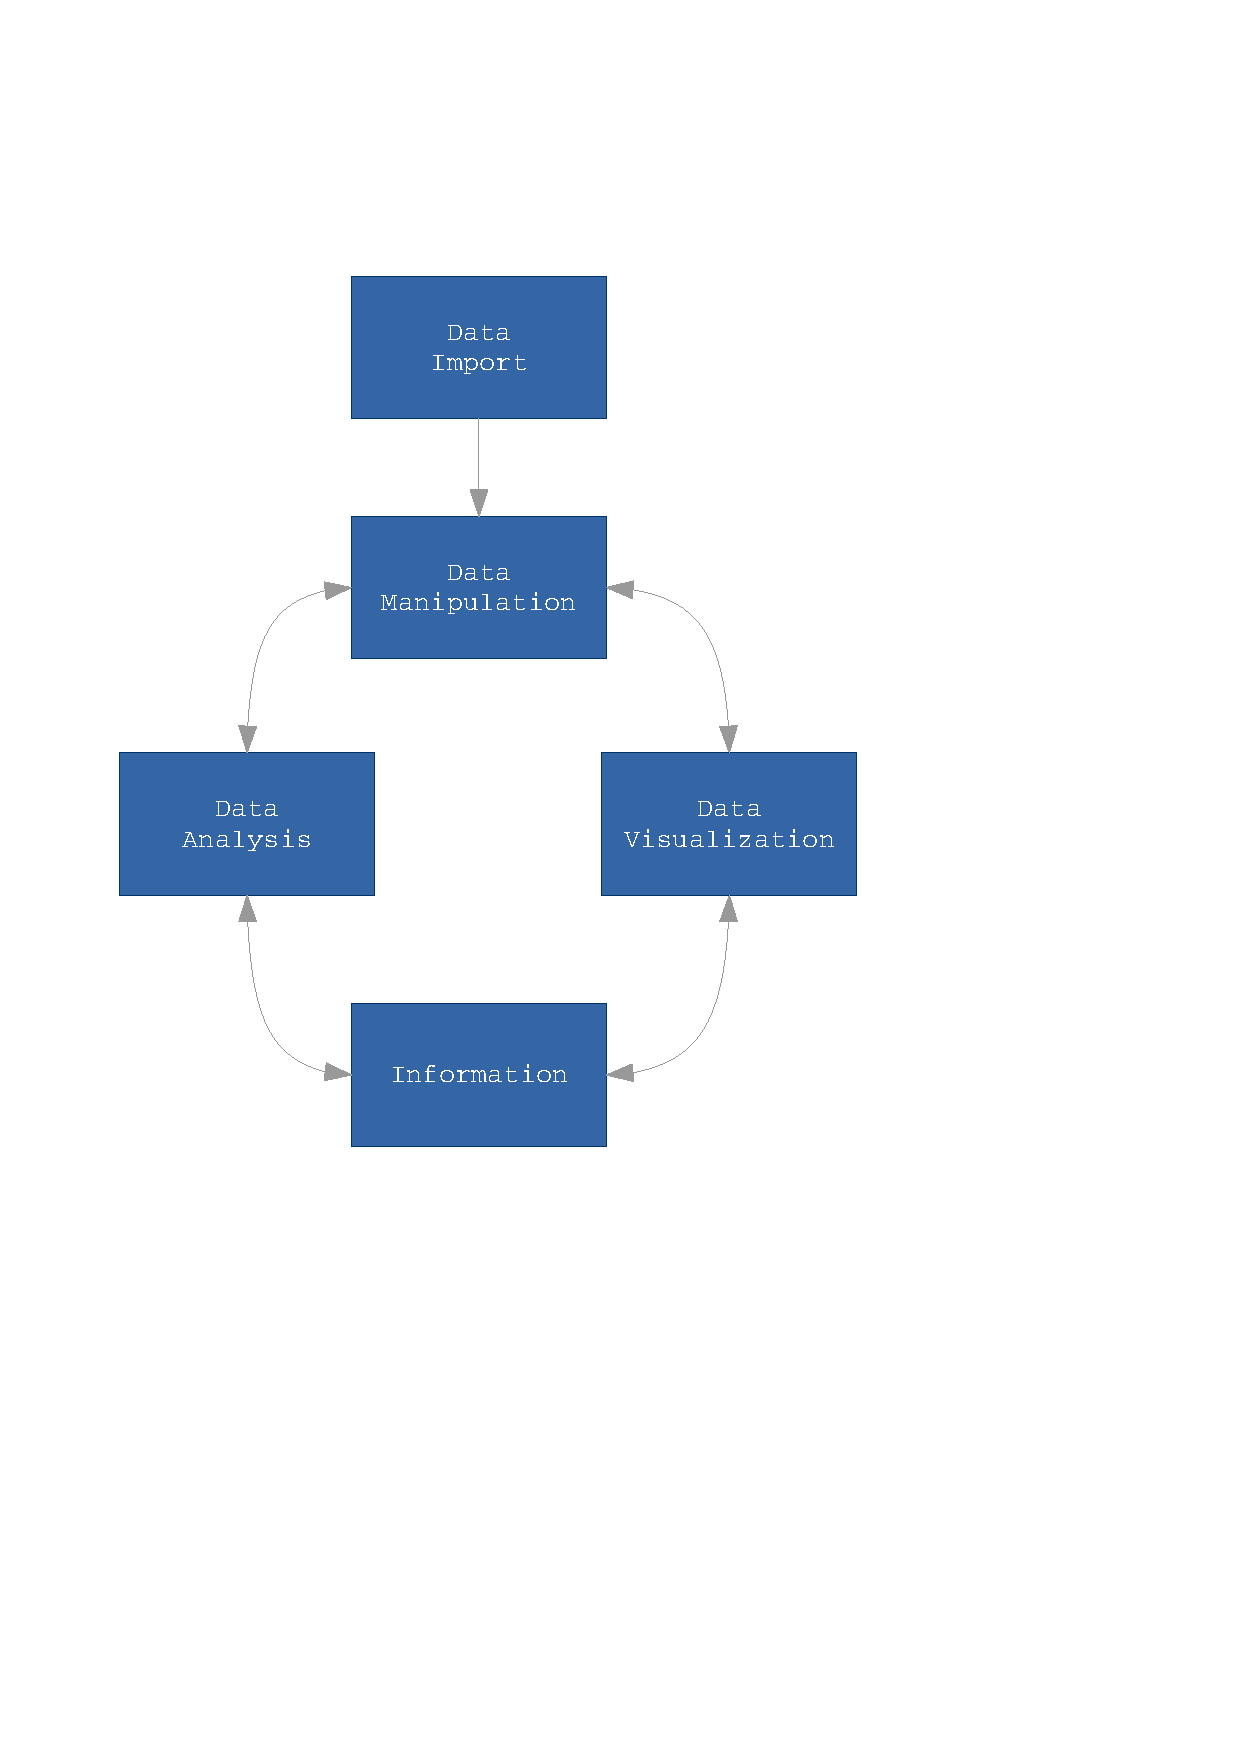
\includegraphics[width=3.6in]{images/flow}

This web book is the result of several years of introductory R courses.
It contains work of my colleagues:

\begin{itemize}
\tightlist
\item
  Daniela Manzato, who wrote the first version of this book,
\item
  Enrico Pegoraro, who wrote chapters about statistical modeling,
\item
  Veronica Giro and Nicola Sturaro, which reviewed and reassembled all
  these materials.
\end{itemize}

\includegraphics[width=5.72in]{images/EF5C8766}

However, it would not have been possible without the sharing of
knowledge, information, ideas, doubts and even criticisms of many
individuals on the internet. I would like to extend my sincere thanks to
all of them.

I am grateful to Bill Venables and John Chambers for their publications
on R that provided solid foundations to my knowledge on this subject.
Moreover \href{http://www.statmethods.net/}{Quick R} often provides some
useful ready-to-cook recipe.

I would finally like to express my special gratitude to Hadley Wickham
for providing and sharing his research on the \texttt{R} packages:
\texttt{dplyr} and \texttt{ggplot2}. Without his contribution, a part of
this manual would never have been written.

I finally express my sincere excuses to all researchers and R
enthusiasts I have borrowed any knowledge from without mentioning them.
This was not intentional, simply I had not always tracked my sources. If
this is the case, please contact me directly and I will be more than
happy to include any appropriate reference in this manual.

Andrea Spanò,\\
Quantide s.r.l.

\chapter{About R}\label{about-r}

\section{R History}\label{r-history}

R is a programming environment for data analysis, graphics and
statistical computing. The R language is widely used among statisticians
for developing statistical software and data analysis.

R was initially developed in early 90s by Robert Gentleman and Ross
Ihaka at the Department of Statistics of the University of Auckland as a
dialect of the S language.

The R name is partly based on the (first) names of the first two R
authors (Robert Gentleman and Ross Ihaka), and partly a play on the name
of S.

\clearpage

\subsection{What is S and a bit of
history}\label{what-is-s-and-a-bit-of-history}

S is a statistical programming language developed by John Chambers and
others in Bell Laboratories.

\begin{figure}[htbp]
\centering
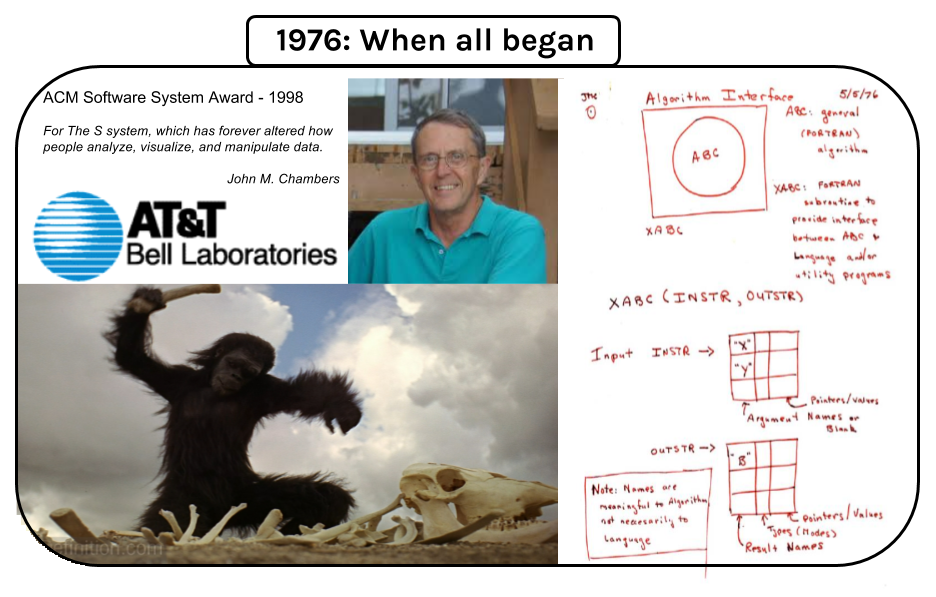
\includegraphics{./images/s-rev.png}
\caption{}
\end{figure}

A bit of history:

\begin{itemize}
\tightlist
\item
  1976: the first version of S is developed as an internal statistical
  analysis environment. It is originally implemented as Fortran
  libraries.
\item
  1980: the first version of S is distributed outside of Bell
  Laboratories. In 1981, source version is made available.
\item
  1984: Richard A. Becker and John M. Chambers, ``S. An Interactive
  Environment for Data Analysis and Graphics''. (Brown Book). Historical
  interest only.
\item
  1988: Richard A. Becker, John M. Chambers and Allan R. Wilks, ``The
  New S Language''. London: Chapman \& Hall. (Blue Book). It introduces
  what is now known as S version 2. The system is rewritten in C and
  begins to resemble the system that we have today.
\item
  1992: John M. Chambers and Trevor J. Hastie, ``Statistical Models in
  S''. (White Book). It introduces S version 3, often abbreviated S3,
  which adds structures to facilitate statistical modeling in S.
\item
  1998: John M. Chambers, ``Programming with Data''. (Green Book). It
  introduces S version 4, often abbreviated S4, which provides advanced
  object-oriented features. S4 classes differ markedly from S3 classes.
\end{itemize}

The S language itself has not changed dramatically since 1998.

\subsection{What is S-PLUS and a bit of
history}\label{what-is-s-plus-and-a-bit-of-history}

S-PLUS is a commercial implementation of the S programming language.

S-PLUS provides a number of fancy features (GUIs, mostly) on top of it,
hence the ``PLUS''.

\begin{figure}[htbp]
\centering

\includegraphics{./images/s+.png}
\caption{}
\end{figure}

A bit of history:

\begin{itemize}
\tightlist
\item
  1993: Statistical Sciences, Inc. acquires the exclusive license to
  distribute S and merges with MathSoft.
\item
  2001: MathSoft sells its Cambridge-based Engineering and Education
  Products Division (EEPD). It changes name to Insightful Corporation.
\item
  2004: Insightful purchases the S language from Lucent Technologies for
  \$2 million.
\item
  2008: TIBCO acquires Insightful Corporation.
\end{itemize}

\clearpage

\subsection{R: a bit of history}\label{r-a-bit-of-history}

\begin{figure}[htbp]
\centering
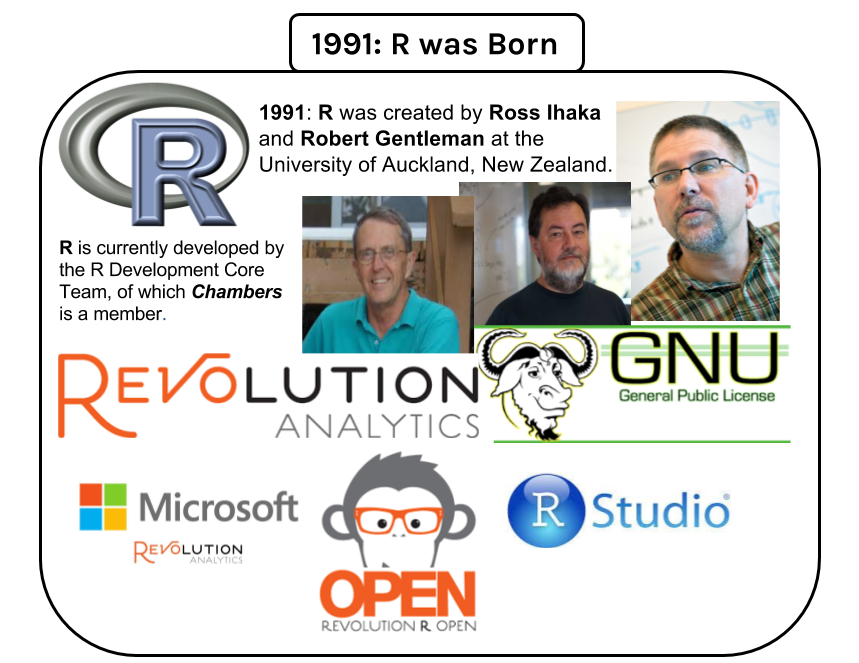
\includegraphics{./images/r.png}
\caption{}
\end{figure}

\begin{itemize}
\tightlist
\item
  1993: First announcement of R to the public.
\item
  1995: Martin Maechler convinces Ross Ihaka and Robert Gentleman to use
  the GNU General Public License to make R free software.
\item
  1997: The R Development Core Team is formed. The team controls the
  source code for R.
\item
  2000: R version 1.0.0 released. Developers consider R stable enough
  for production use.
\item
  2004: R version 2.0.0 released. Introduced lazy loading, which enables
  fast loading of data with minimal expense of system memory.
\item
  2013: R version 3.0.0 released. Introduced long vectors.
\end{itemize}

While R is an open source project supported by the community developing
it, some companies strive to provide commercial support and/or
extensions for their customers. R history is intertwined with that of
its commercial support:

\begin{itemize}
\tightlist
\item
  2007: Revolution Analytics was founded to provide commercial support
  for Revolution R, the distribution of R developed by Revolution
  Analytics which also includes components developed by the company.
\item
  2010: RStudio was founded. It is a company that develops free and open
  tools for the R community.
\item
  2014: Microsoft Corporation starts the release of Microsoft R Open, an
  enhanced distribution of R, formerly known as Revolution R Open (RRO).
\item
  2015: Microsoft Corporation completed the acquisition of Revolution
  Analytics.
\end{itemize}

We will deepen the commercial support tools mentioned in \emph{R
commercial support} paragraph.

In April 2016, R is in 18th place of TIOBE Programming Community Index,
that is an indicator of the popularity of programming languages. R is
above SAS that is in 23th place.

\section{The R-project and R Licence}\label{the-r-project-and-r-licence}

R is supported by a wide community of academic users, professors,
companies and developers. This community composes the so-called
``R-project''. The ``R-project'' is supported by the ``R Foundation''.
The R Foundation is a not for profit organisation.

R is an official part of the Free Software Foundation's GNU project. The
R Foundation has similar goals to other open source software foundations
like the Apache Foundation or the GNOME Foundation. R is free and open
source software. It is released under the GPL (version 2) licence.

R is free:

\begin{itemize}
\tightlist
\item
  you can have R without paying for it (freeware);
\item
  you can copy and re-use the software (free software);
\item
  you can access source code and modify it (open source).
\end{itemize}

\subsection{What R does?}\label{what-r-does}

R provides a suite of software facilities for:

\begin{itemize}
\tightlist
\item
  matrix algebra;
\item
  hash tables and regular expressions;
\item
  reading and manipulating data;
\item
  computation;
\item
  programming language: loops, subroutines, functions, etc.;
\item
  conducting statistical analyses;
\item
  graphics and tables;
\item
  displaying the results.
\end{itemize}

On the contrary, R:

\begin{itemize}
\tightlist
\item
  it is not a database, but it connects to databases;
\item
  it does not provide a graphical interface, but it uses Java, TclTk
  and, under Windows, COM to provide graphical interfaces;
\item
  it is not a spreadsheet, but it connects to spreadsheets;
\item
  it does not provide commercial support. Revolution R is a commercially
  supported distribution of R.
\end{itemize}

In conclusion, R is an interpreted computer language. R provides a
platform for the development and implementation of new algorithms and
technology transfer. Most user-visible functions are written in R
itself, calling upon a smaller set of internal primitives. It is
possible to interface procedures written in C, C+, or FORTRAN languages
for efficiency, and to write additional primitives. System commands can
be called from within R.

\subsubsection{R Advantages and
Disadvantages}\label{r-advantages-and-disadvantages}

Main R advantages are:

\begin{itemize}
\tightlist
\item
  Fast and free.
\item
  State of the art: Statistical researchers provide their methods as R
  packages. SPSS and SAS are years behind R!
\item
  Excellent for graphics.
\item
  Mx, WinBugs, and other programs use or will use R.
\item
  Active user community.
\item
  Excellent for simulation, programming, computer intensive analyses,
  etc.
\item
  Forces you to think about your analysis.
\item
  Interfaces with database storage software (SQL).
\end{itemize}

Main R disadvantages are:

\begin{itemize}
\tightlist
\item
  Not user friendly at start: steep learning curve, minimal GUI.
\item
  Sometimes, figuring out correct methods or how to use a function on
  your own can be frustrating.
\item
  Easy to make mistakes and not know.
\item
  Working with large datasets is limited by RAM.
\item
  Data preparation and cleaning can be messier and more mistake prone in
  R vs SPSS or SAS.
\end{itemize}

\clearpage

\section{R Online Resources}\label{r-online-resources}

R strength is its community, which is distributed and keeps growing all
over the World!

\begin{figure}[htbp]
\centering
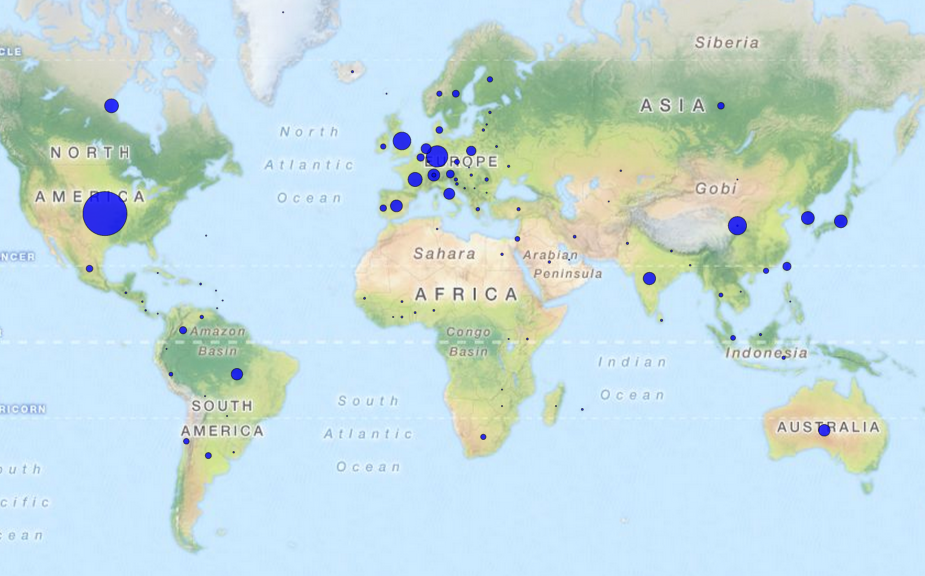
\includegraphics{./images/r-users-distribution.png}
\caption{}
\end{figure}

Thanks to its community, R can boast a wide variety of online resources,
free and otherwise, to learn more about it, ranging from websites, blogs
and commercial support tools.

Let us have a look at the most important.

\subsection{R-project Website}\label{r-project-website}

The R-project website
\href{http://www.r-project.org/}{(www.r-project.org)} is the starting
point for R materials.

The website contains:

\begin{itemize}
\tightlist
\item
  the software and packages;
\item
  the search engine interface (the same queries can be submitted with
  the RSiteSearch (`query') function within R);
\item
  the on-line documentation both in HTML and in PDF format. The HTML
  version can be accessed with the \texttt{help.start()} function within
  R;
\item
  the R Journal. The R Journal is the open access, refereed journal of
  the R project. It features short to medium length articles covering
  topics that might be of interest to users or developers of R;
\item
  the interface to the mailing list;
\item
  the wiki, suggested books and many others.
\end{itemize}

The on-line documentation includes the following manuals. These manuals
have been written by the R Development Core Team itself and contain
precious information.

\begin{itemize}
\tightlist
\item
  \emph{An Introduction to R} gives an introduction to the language and
  how to use R for doing statistical analysis and graphics.
\item
  \emph{Writing R Extensions} covers how to create your own packages,
  write R help files, and the foreign language (C, C++, Fortran,
  \ldots{}) interfaces.
\item
  \emph{R Data Import/Export} describes the import and export facilities
  available either in R itself or via packages which are available from
  CRAN.
\item
  \emph{R Installation and Administration}.
\end{itemize}

Other manuals and tutorials provided by R users can be downloaded from
the R-project website
\href{http://cran.r-project.org/other-docs.html}{(cran.r-project.org/other-docs.html)}.

Mailing lists is the most important tool to contact the R community.
Mailing lists can be accessed from the R-project website
\href{http://www.r-project.org/mail.html}{(www.r-project.org/mail.html)}.

There are five general mailing lists devoted to R:

\begin{itemize}
\tightlist
\item
  \emph{R-announce}: This list is for major announcements about the
  development of R and the availability of new code.
\item
  \emph{R-packages}: This list is for announcements as well, usually on
  the availability of new or enhanced contributed packages (on CRAN,
  typically).
\item
  \emph{R-help}: The ``main'' R mailing list, for discussion about
  problems and solutions using R, announcements about the availability
  of new functionality for R and documentation of R, comparison and
  compatibility with S-plus, and for the posting of nice examples and
  benchmarks.
\item
  \emph{R-devel}: This list is intended for questions and discussion
  about code development in R.
\item
  \emph{R-package-devel}: This list is to get help about package
  development in R.
\end{itemize}

\subsection{Other Online Resources}\label{other-online-resources}

It is very difficult estimate how many sites about R are on-line.
However, Google returns 224.000.000 sites searching ``R stat blog''.
Also if only the 0.1\% of these sites talk about R, it means almost
220.000 sites about R.

R-bloggers \href{http://www.r-bloggers.com/}{(www.r-bloggers.com)} is a
blog aggregator of content collected from bloggers who write about R.
R-bloggers contains R news and tutorials contributed by hundreds of R
bloggers.

We suggest you to visit MilanoR
\href{http://www.milanor.net/}{(www.milanor.net)}, which is the blog of
R users in the Milan Area. Its aim is to exchange knowledge, learn and
share tricks and techniques and provide R beginners with an opportunity
to meet more experienced users.

Other useful websites about R are:

\begin{itemize}
\tightlist
\item
  Stack Overflow
  \href{http://stackoverflow.com/}{(www.stackoverflow.com)} is a website
  that features questions and answers on a wide range of topics in
  computer programming, among which r.
\item
  Quick-R \href{http://www.statmethods.net/}{(www.statmethods.net)} is a
  useful on-line guide to R. It provides many examples and useful tips.
\item
  R seek \href{http://rseek.org/}{(rseek.org)} uses Google to search in
  a selected list of websites about R.
\end{itemize}

\subsection{R Commercial Support}\label{r-commercial-support}

\subsubsection{RStudio Inc.}\label{rstudio-inc.}

RStudio, Inc. \href{http://www.rstudio.com/}{(www.rstudio.com)} is a
company that develops free and open tools for the R community, inspired
by the innovations of R users in science, education, and industry. These
include the RStudio development environment as well as the
\texttt{shiny}, \texttt{ggvis}, and \texttt{dplyr} packages (among many
others).

RStudio has a mission to provide the most widely used open source and
enterprise-ready professional software for the R statistical computing
environment. These tools will further the cause of expanding the use of
R and the field of data science. It also offers open source and
enterprise ready tools for the R computing environment. The flagship
product of the RStudio team is an Integrated Development Environment
(IDE) which makes it easy for analysts, scientists, data scientists and
quants to perform their analyses. It also offer Shiny: a platform that
allows you to take those analyses and share them with your
team/organization by creating interactive web applications.

\subsubsection{Microsoft Corporation}\label{microsoft-corporation}

Microsoft Corporation provides Microsoft R Open
\href{https://mran.microsoft.com/open/}{www.mran.microsoft.com/open}, an
enhanced distribution of R, formerly known as Revolution R Open (RRO).
It is a complete open source platform for statistical analysis and data
science. The current version, Microsoft R Open 3.3.2, is based on (and
100\% compatible with) R-3.3.2 and is therefore fully compatibility with
all packages, scripts and applications that work with that version of R.
It includes additional capabilities for improved performance,
reproducibility, as well as support for Windows and Linux-based
platforms. Like R, Microsoft R Open is open source and free to download,
use, and share. It is available for Windows, Linux and Mac Os operative
systems and you can download it
\href{https://mran.microsoft.com/download/}{here}.

\chapter{R and RStudio Set Up}\label{r-and-rstudio-set-up}

\section{Installing and Updating R}\label{installing-and-updating-r}

\subsection{Design of the R System}\label{design-of-the-r-system}

The R system is divided into two conceptual parts:

\begin{enumerate}
\def\labelenumi{\arabic{enumi}.}
\tightlist
\item
  The ``base'' R system that you download from CRAN.
\item
  Everything else.
\end{enumerate}

R functionality is divided into a number of packages. The ``base'' R
system contains, among other things, the \emph{base} package which is
required to run R and contains the most fundamental functions. The
``base'' system contains also some other packages. Furthermore, every R
installation contains ``recommended'' packages, that are not necessarily
maintained by R Core.

``Everything else'' point out CRAN ``contributed'' packages and packages
that are not on CRAN. This does not mean that these packages are
necessarily of lesser quality than the above, e.g., many contributed
packages on CRAN are written and maintained by R Core members. The goal
is simply to try to keep the base distribution as lean as possible.
Beyond CRAN, many packages are avalaible in BioConductor project or in
Github repositories.

\subsection{Installing R}\label{installing-r}

R is available for Windows, Mac Os and Linux.

The base R can be downloaded from the Comprehensive R Archive Network
(CRAN) website. The CRAN is a collection of sites which carry identical
material, consisting of the R distribution(s), the contributed
extensions, documentation for R, and binaries.

Go to \href{http://www.r-project.org/}{www.r-project.org}. Here you can
read about R and see what's new in the latest version.

\hypertarget{fig:ssSiteRproject}{}
\begin{figure}[htbp]
\centering
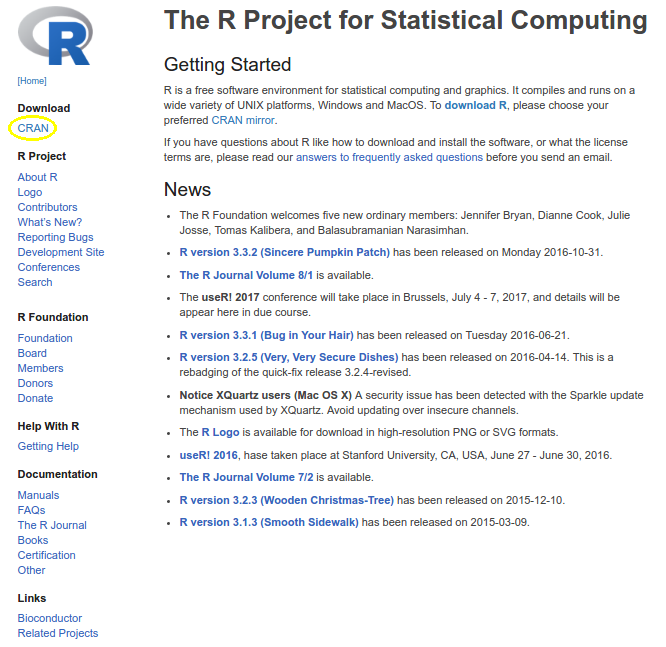
\includegraphics{./images/r-project.png}
\caption{Screenshot of the R-project website\label{fig:ssSiteRproject}}
\end{figure}

Click on CRAN under Download in the left list (see Figure
\protect\hyperlink{fig:ssSiteRproject}{Screenshot of the R-project
website}). That'll take you to a list of servers (mirrors) in different
countries where you can download R.

Now you can choose what operative system you have. Choose within the
upper box with ``Download and Install R''. The box contains
``Precompiled binary distributions''; sounds complicated, but means that
the program is ready to use, with installation program and all.

Windows users click on ``base'' and then click ``Download R X.X.X for
Windows''.

Mac users click on ``R-X.X.X.pkg (latest version)''.

Linux users find download files and installation instructions for their
Linux distribution in the website.

X.X.X identify the current version of R. In December 2016, the current
version is the 3.3.2.

To install R, Windows and Mac users must just double click on the file
and follow the installation instructions.

Linux users can download and install R using the precompiled R binary
for their distribution. Alternatively, experienced Linux users can
compile R from sources. Currently, precompiled R binary are available
for Debian, Ubuntu, Suse and RedHat. The R installation package for
RedHat downloadable from CRAN is obsolete. An R updated version for Red
Hat Enterprise Linux 5 is available for free by Revolution Analytics.

The Figure \protect\hyperlink{fig:ssFirsttry}{Screenshot of a first try
with R} shows a first try with R, just after installation.

\hypertarget{fig:ssFirsttry}{}
\begin{figure}[htbp]
\centering
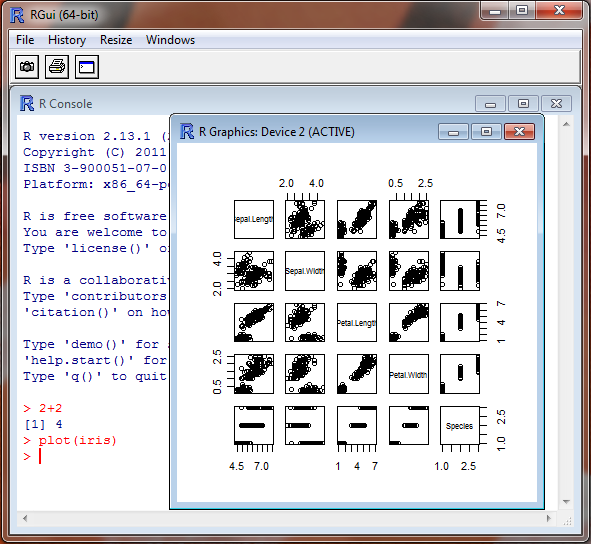
\includegraphics{./images/RfirstPlot.png}
\caption{Screenshot of a first try with R\label{fig:ssFirsttry}}
\end{figure}

\clearpage

\subsection{Updating R}\label{updating-r}

In Windows and Mac, there is not an automatic way to update R. Two or
more versions of R can coexist in the same machine, so a newer release
of R can be installed beside the old release. Unfortunately, packages
must be re-installed in the ``new'' R version. A copy-and-paste of
package files from the directory containing the packages of the ``old''
R version to the directory containing the packages of the ``new'' R
version may be useful when many packages are installed. Within R, the
\texttt{.Library} variable shows the directory containing the packages.
After the copy-and-paste, packages of the ``new'' R version should be
updated.

In Linux, usually one R version at time can be installed. R can be
updated following the instructions in the CRAN website.

\section{Graphical User Interfaces}\label{graphical-user-interfaces}

\subsection{R Default Interfaces}\label{r-default-interfaces}

R is provided with a Command Line Interface (CLI), which is the
preferred user interface for power users because it allows direct
control on calculations and it is flexible. However, good knowledge of
the language is required. CLI is thus intimidating for beginners. The
learning curve is typically longer than with a Graphical User Interface
(GUI), although it is recognised that the effort is profitable and leads
to better practice (finer understanding of the analysis, command easily
saved and replayed).

R is available for many different operative systems so it does not
provide the same graphical interface. When you use the R program
interactively, it issues a prompt when it expects input commands. The
default prompt is `\textgreater{}'. In Windows, RGui is the default GUI.
Inside RGui there is the RConsole window. In Macintosh, RConsole is the
default GUI. In Linux, R does not provide any graphical interface by
default and it can be used through CLI.

\begin{figure}[htbp]
\centering
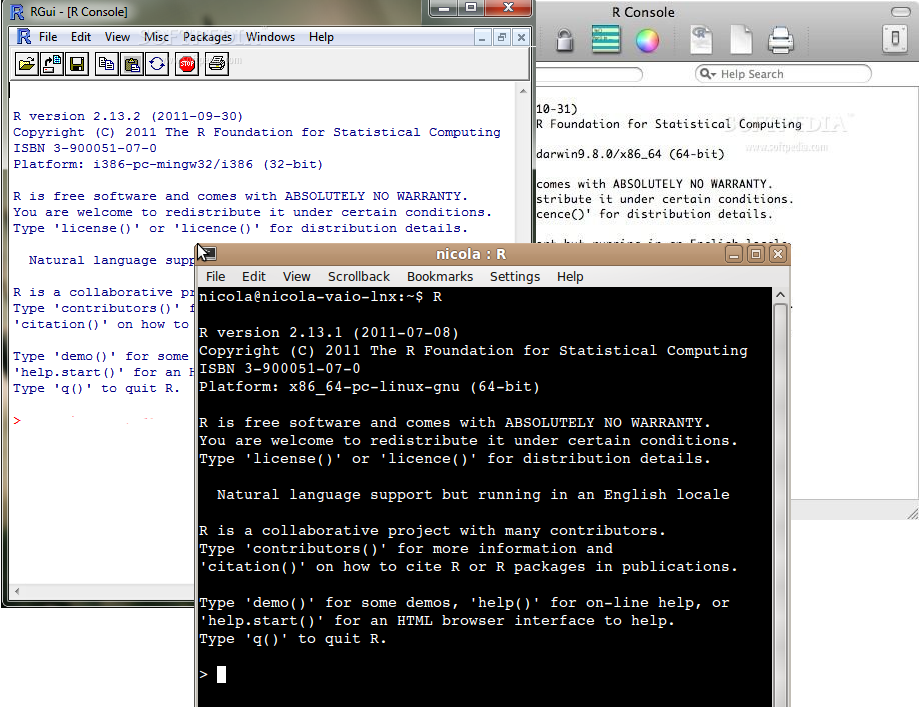
\includegraphics{images/ssDefaultGui.png}
\caption{}
\end{figure}

\clearpage

\subsection{RStudio and Others R Alternate
Interfaces}\label{rstudio-and-others-r-alternate-interfaces}

Several projects develop or offer the opportunity to develop alternate
user interfaces. They are presented at
\href{http://www.sciviews.org/_rgui/}{www.sciviews.org/\_rgui}.

\textbf{RStudio} \href{http://www.rstudio.org/}{(www.rstudio.org)} is a
free and open source multi-platform integrated development environment
(IDE) for R. It provides syntax highlighting, code completion and smart
indentation. Moreover, it executes R code directly from the source
editor and it manages easily multiple working directories using
projects. It provides:

\begin{itemize}
\tightlist
\item
  workspace browser and data viewer;
\item
  plot history, zooming, and flexible image and PDF export;
\item
  integrated R help and documentation;
\item
  Sweave authoring including one-click PDF preview;
\item
  searchable command history.
\end{itemize}

\begin{figure}[htbp]
\centering
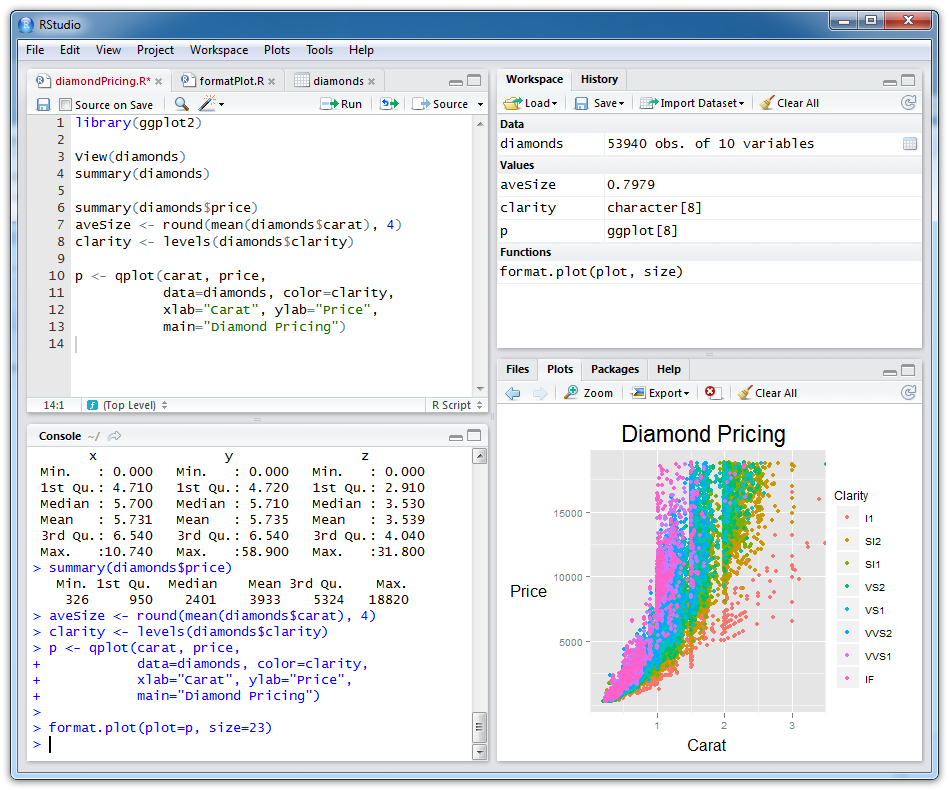
\includegraphics{images/ssGuiRstudio.png}
\caption{}
\end{figure}

\clearpage

RStudio is available for Windows, Mac Os and Linux and you can install
it from its website \href{http://www.rstudio.org/}{(www.rstudio.org)},
clicking on \emph{Download RStudio}. Next, click \emph{Download RStudio
Desktop}. At this stage, click the link to the version of RStudio
appropriate for your system in \emph{Installers for Supported Platforms}
section. Clicking this link downloads RStudio to your computer. Run the
installation file and RStudio will be installed on your system.

Similarly to RStudio, \textbf{JGR}
\href{http://rforge.net/JGR/}{(rforge.net/JGR)} and \textbf{Rkward}
\href{http://rkward.sourceforge.net/}{(rkward.sourceforge.net)} are
multi-platform IDE. JGR is an R console replacement, it provides also a
very decent R code editor with syntax highlighting, calltips, completion
and submission of code to R. Rkward has interesting features too to edit
R script files and submit code to R.

\begin{figure}[htbp]
\centering
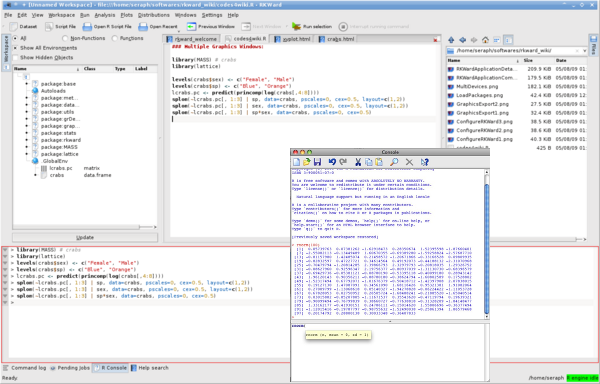
\includegraphics{images/ssGuiJgr.png}
\caption{}
\end{figure}

\clearpage

\textbf{Tinn-R}
\href{http://www.sciviews.org/Tinn-R/}{(www.sciviews.org/Tinn-R)} is one
of the most used R editor by Windows users. It includes R syntax
highlighting, help on R functions syntax while you type them, direct
submission of R code and many other tools to control R from within the
editor.

\begin{figure}[htbp]
\centering
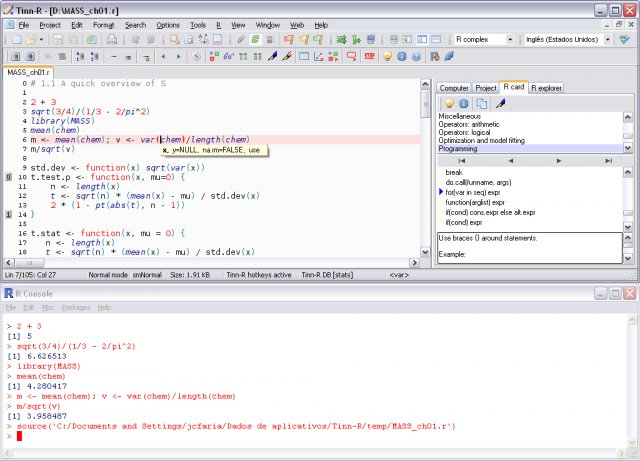
\includegraphics{images/ssGuiTinnr.jpg}
\caption{}
\end{figure}

\clearpage

\textbf{Emacs}, \textbf{VIM}, \textbf{Eclipse} and \textbf{Komodo} are
powerful multiplatform editors well known by software developers. They
support also R, directly or through plugins.

\begin{figure}[htbp]
\centering
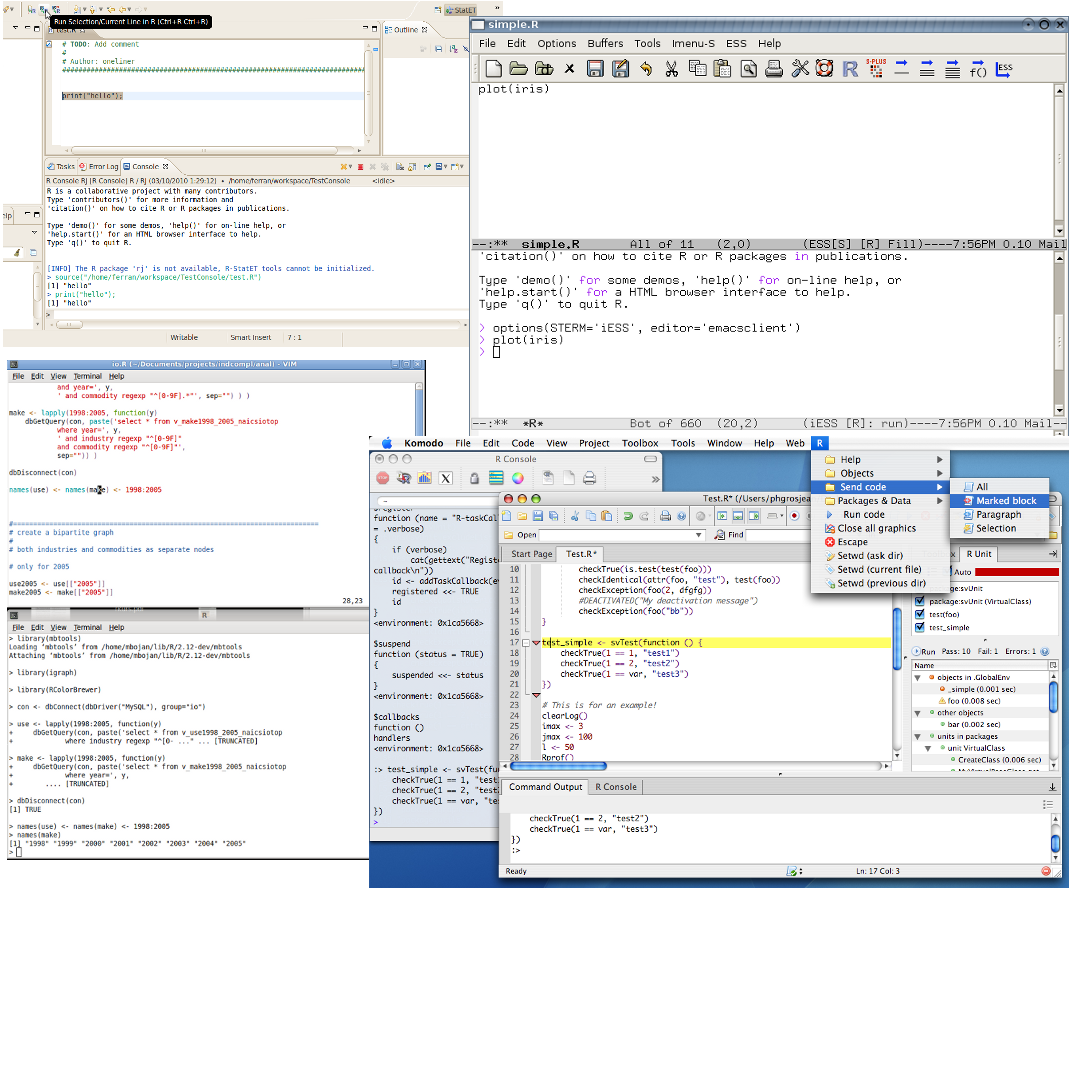
\includegraphics{images/ssGuiEmacs.png}
\caption{}
\end{figure}

\begin{figure}[htbp]
\centering
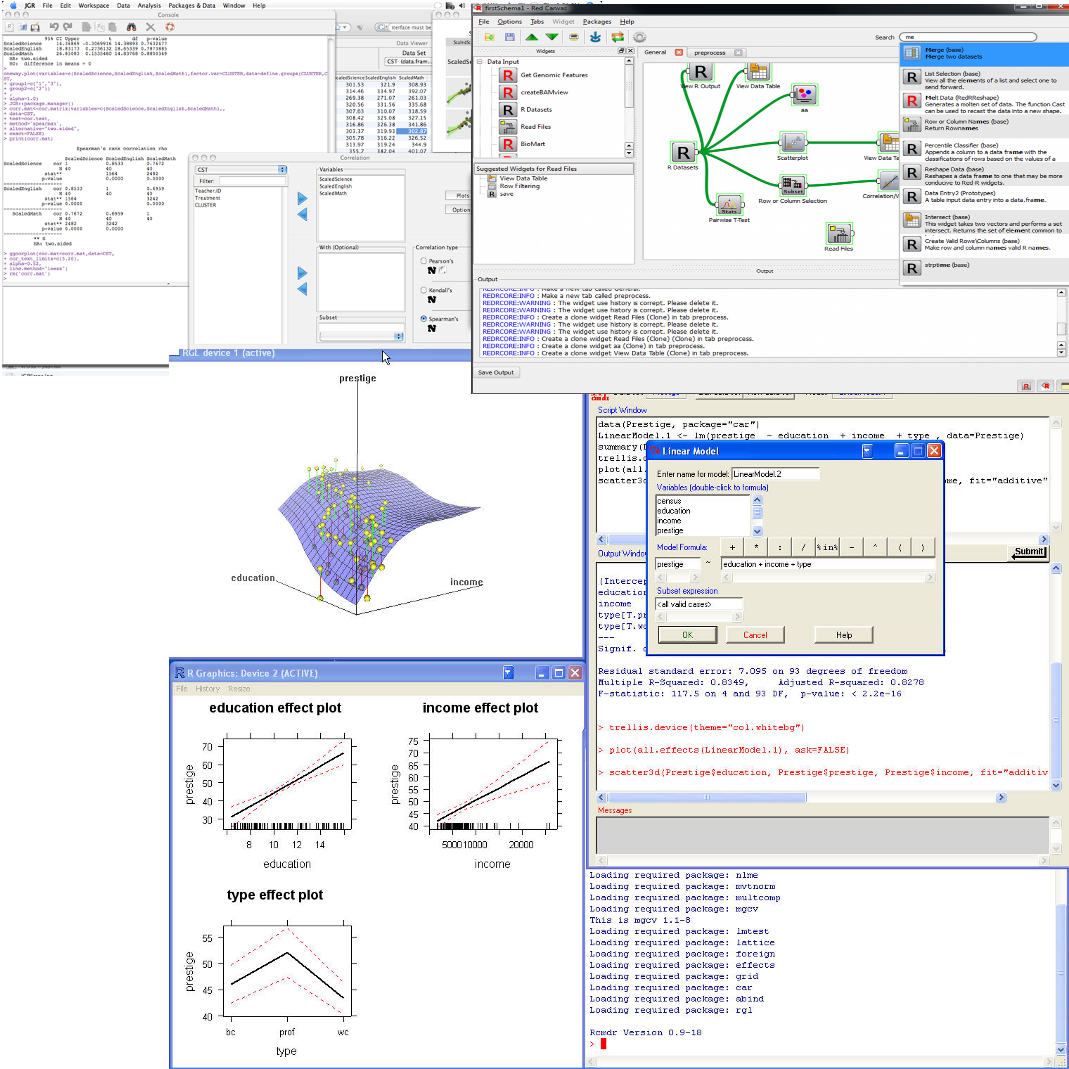
\includegraphics{images/ssGuiDeducer.png}
\caption{}
\end{figure}

\clearpage

GUIs and IDEs are designed to facilitate programming. Several projects
try to provide a graphical interface to R, with menu and buttons:

\begin{itemize}
\tightlist
\item
  \textbf{Deducer} \href{http://www.deducer.org/}{(www.deducer.org)} is
  designed to be a free easy to use alternative to proprietary data
  analysis software. It has a menu system to do common data manipulation
  and analysis tasks, and an excel-like spreadsheet in which to view and
  edit data frames. It provides an intuitive graphical user interface
  (GUI) for R, encouraging non-technical users to learn and perform
  analyses without programming getting in their way. Deducer is designed
  to be used with the Java based R console JGR.
\item
  \textbf{R-Commander}
  \href{http://socserv.mcmaster.ca/jfox/Misc/Rcmdr/}{(socserv.mcmaster.ca/jfox/Misc/Rcmdr)},
  or Rcmdr, provides also access to the most frequently used statistical
  tools through the mouse.
\item
  \textbf{Red-R} \href{http://www.red-r.org/}{(www.red-r.org)} is a
  dataflow programming interface for R designed to bring the power of
  the R statistical environment to the general researcher or user.
\end{itemize}

\clearpage

\section{R Packages}\label{r-packages}

\subsection{Installing R Packages}\label{installing-r-packages}

R functions are collected in packages. Packages that are not contained
in the ``base'' R systems can be downloaded from the CRAN website. A
list of R packages accompanied by a brief description can be found on
the CRAN website where there are more than 3700 packages available. Many
of these packages are very useful; however, there are some packages in
prerelease, incomplete packages, ``abandoned'' packages (i.e.~not more
updated) and/or packages containing functions with errors or
compatibility troubles.

This is the R package universe!

\begin{figure}[htbp]
\centering

\includegraphics{./images/r-packages-universe.png}
\caption{}
\end{figure}

The simple way to install an R package is through the
\texttt{install.packages()} function, directly from R. In Linux, R must
be executed as administrator to install a package. Installation must be
executed before the first use of a library.

When a function of a package that is not contained in the ``base'' R
systems is required than the package must be loaded. The
\texttt{require(pkg)} function load the \emph{pkg} package.

\subsection{Updating R Packages}\label{updating-r-packages}

R packages can be updated typing \texttt{update.packages()} within R. In
Linux, R must be executed as administrator to update a package. Packages
should be updated regularly.

\chapter{A First Look to R Session}\label{a-first-look-to-r-session}

\section{The First R Session}\label{the-first-r-session}

Start the R system, the cursor is waiting for you to type in some R
commands. For example, use R as a simple calculator:

\begin{Shaded}
\begin{Highlighting}[]
\DecValTok{6} \NormalTok{+}\StringTok{ }\DecValTok{3}
\end{Highlighting}
\end{Shaded}

\begin{verbatim}
## [1] 9
\end{verbatim}

\begin{Shaded}
\begin{Highlighting}[]
\DecValTok{5} \NormalTok{-}\StringTok{ }\DecValTok{9}
\end{Highlighting}
\end{Shaded}

\begin{verbatim}
## [1] -4
\end{verbatim}

\begin{Shaded}
\begin{Highlighting}[]
\DecValTok{4} \NormalTok{*}\StringTok{ }\DecValTok{6}
\end{Highlighting}
\end{Shaded}

\begin{verbatim}
## [1] 24
\end{verbatim}

\begin{Shaded}
\begin{Highlighting}[]
\DecValTok{8} \NormalTok{/}\StringTok{ }\DecValTok{3}
\end{Highlighting}
\end{Shaded}

\begin{verbatim}
## [1] 2.666667
\end{verbatim}

\begin{Shaded}
\begin{Highlighting}[]
\DecValTok{5} \NormalTok{^}\StringTok{ }\DecValTok{2}
\end{Highlighting}
\end{Shaded}

\begin{verbatim}
## [1] 25
\end{verbatim}

\begin{Shaded}
\begin{Highlighting}[]
\NormalTok{(}\DecValTok{1} \NormalTok{+}\StringTok{ }\FloatTok{0.05}\NormalTok{)^}\DecValTok{8}
\end{Highlighting}
\end{Shaded}

\begin{verbatim}
## [1] 1.477455
\end{verbatim}

\begin{Shaded}
\begin{Highlighting}[]
\KeywordTok{exp}\NormalTok{(}\DecValTok{3}\NormalTok{)}
\end{Highlighting}
\end{Shaded}

\begin{verbatim}
## [1] 20.08554
\end{verbatim}

\begin{Shaded}
\begin{Highlighting}[]
\KeywordTok{log}\NormalTok{(}\DecValTok{14}\NormalTok{)}
\end{Highlighting}
\end{Shaded}

\begin{verbatim}
## [1] 2.639057
\end{verbatim}

\begin{Shaded}
\begin{Highlighting}[]
\FloatTok{23.76} \NormalTok{*}\StringTok{ }\KeywordTok{log}\NormalTok{(}\DecValTok{8}\NormalTok{)/(}\DecValTok{23} \NormalTok{+}\StringTok{ }\KeywordTok{atan}\NormalTok{(}\DecValTok{9}\NormalTok{))}
\end{Highlighting}
\end{Shaded}

\begin{verbatim}
## [1] 2.01992
\end{verbatim}

\section{Assignment}\label{assignment}

Results of calculations can be stored in objects using the assignment
operators:

\begin{itemize}
\tightlist
\item
  an arrow (\texttt{\textless{}-}) formed by a smaller than character
  and a hyphen without a space;
\item
  the equal character (\texttt{=}).
\end{itemize}

These objects can then be used in other calculations.

There are some restrictions when giving an object a name:

\begin{itemize}
\tightlist
\item
  Object names cannot contain ``strange'' symbols like \texttt{!},
  \texttt{+}, \texttt{-}, \texttt{\#}.
\item
  A dot (\texttt{.}) and an underscore (\texttt{\_}) are allowed, also a
  name starting with a dot.
\item
  Object names can contain a number but cannot start with a number.
\item
  R is case sensitive: \texttt{X} and \texttt{x} are two different
  objects, as well as \texttt{temp} and \texttt{temP}.
\end{itemize}

\begin{Shaded}
\begin{Highlighting}[]
\NormalTok{x <-}\StringTok{ }\KeywordTok{log}\NormalTok{(}\DecValTok{14}\NormalTok{)}
\NormalTok{y <-}\StringTok{ }\FloatTok{23.76} \NormalTok{*}\StringTok{ }\KeywordTok{log}\NormalTok{(}\DecValTok{8}\NormalTok{)/(}\DecValTok{23} \NormalTok{+}\StringTok{ }\KeywordTok{atan}\NormalTok{(}\DecValTok{9}\NormalTok{))}
\NormalTok{z <-}\StringTok{ }\NormalTok{x +}\StringTok{ }\NormalTok{y}
\end{Highlighting}
\end{Shaded}

To print the object just enter the name of the object or use
\texttt{print()} function.

\begin{Shaded}
\begin{Highlighting}[]
\NormalTok{x}
\end{Highlighting}
\end{Shaded}

\begin{verbatim}
## [1] 2.639057
\end{verbatim}

\begin{Shaded}
\begin{Highlighting}[]
\NormalTok{y}
\end{Highlighting}
\end{Shaded}

\begin{verbatim}
## [1] 2.01992
\end{verbatim}

\begin{Shaded}
\begin{Highlighting}[]
\KeywordTok{print}\NormalTok{(z)}
\end{Highlighting}
\end{Shaded}

\begin{verbatim}
## [1] 4.658978
\end{verbatim}

\section{The R Workspace}\label{the-r-workspace}

The workspace is your current R working environment and includes any
user-defined objects. It is also known as global environment.

\subsection{Objects listing}\label{objects-listing}

Objects created during an R session are hold in memory. To list the
objects in the current R session, the function \texttt{ls()} or the
function \texttt{objects()} may be used.

\begin{Shaded}
\begin{Highlighting}[]
\KeywordTok{ls}\NormalTok{()}
\end{Highlighting}
\end{Shaded}

\begin{verbatim}
## [1] "x" "y" "z"
\end{verbatim}

\begin{Shaded}
\begin{Highlighting}[]
\KeywordTok{objects}\NormalTok{()}
\end{Highlighting}
\end{Shaded}

\begin{verbatim}
## [1] "x" "y" "z"
\end{verbatim}

So to run the function \texttt{ls} the name followed by an opening and a
closing bracket must be entered. Entering only \texttt{ls} will just
print the object, i.e.~the underlying R code of the function.

Most functions in R accept certain arguments. For example, one of the
arguments of the function \texttt{ls()} is pattern. To list all objects
starting with the letter \texttt{x}:

\begin{Shaded}
\begin{Highlighting}[]
\NormalTok{x2 <-}\StringTok{ }\KeywordTok{log}\NormalTok{(}\DecValTok{9}\NormalTok{)}
\KeywordTok{ls}\NormalTok{(}\DataTypeTok{pattern =} \StringTok{"x"}\NormalTok{)}
\end{Highlighting}
\end{Shaded}

\begin{verbatim}
## [1] "x"  "x2"
\end{verbatim}

\subsection{Removing objects}\label{removing-objects}

If a value to an object that already exists is assigned then the
contents of the object will be overwritten with the new value (without a
warning!). The function \texttt{rm()} ought be used to remove one or
more objects from your session.

\begin{Shaded}
\begin{Highlighting}[]
\KeywordTok{rm}\NormalTok{(x2)}
\KeywordTok{ls}\NormalTok{()}
\end{Highlighting}
\end{Shaded}

\begin{verbatim}
## [1] "x" "y" "z"
\end{verbatim}

\subsection{Garbage collection}\label{garbage-collection}

When objects are no longer used, and this clearly happens when objects
are deleted, \texttt{R} releases immediately the memory they filled in
the system. This is done automatically by the garbage collector
\texttt{gc()}.

We can call \texttt{gc()} also to see how much memory \texttt{R} is
using for allocating objects

\begin{Shaded}
\begin{Highlighting}[]
\KeywordTok{gc}\NormalTok{()}
\end{Highlighting}
\end{Shaded}

\begin{verbatim}
##          used (Mb) gc trigger (Mb) max used (Mb)
## Ncells 412003 22.1     750400 40.1   592000 31.7
## Vcells 590174  4.6    1308461 10.0   812630  6.2
\end{verbatim}

\section{The Working Directory}\label{the-working-directory}

If you want to read files from a specific location or write files to a
specific location without typing (on Windows, usually very long) path
names you will need to set working directory in R.

You can set a working directory with \texttt{setwd()} function, using
absolute or relative paths. The following example shows how to set the
working directory in R using an absolute path. The working directory is
set to the folder ``Data'' within the folder ``Documents and Settings''
on the C drive.

\begin{Shaded}
\begin{Highlighting}[]
\KeywordTok{setwd}\NormalTok{(}\StringTok{"C:/User/Andrea/Documents and Settings/Data"}\NormalTok{)}
\end{Highlighting}
\end{Shaded}

Remember that you must use the forward slash / or double backslash
\textbackslash{}\textbackslash{} in R! The Windows format of single
backslash will not work.

It is a nice approach, but things get complicated if you move files to
different computers, say from home to your office, and have different
directory structures, disk names etc. Of course you can change it every
time. Using relative paths solves this problem. Relative paths are more
convenient than absolute paths as they makes your R script or RStudio
project independent of the directory structure in which it resides thus
facilitating the reproducibility of your work on a different PC.

So, you can use \texttt{getwd()} function to get the path of the current
working directory:

\begin{Shaded}
\begin{Highlighting}[]
\KeywordTok{getwd}\NormalTok{()}
\end{Highlighting}
\end{Shaded}

\begin{verbatim}
## [1] "C:/User/Andrea/Documents and Settings/Data"
\end{verbatim}

Suppose that your current directory is the previous one (``Data''
folder) and you want to set the directory on ``Statistics'' folder
inside ``Data'' folder:

\begin{Shaded}
\begin{Highlighting}[]
\KeywordTok{setwd}\NormalTok{(}\StringTok{"./Statistics"}\NormalTok{)}
\end{Highlighting}
\end{Shaded}

\begin{verbatim}
## [1] "C:/User/Andrea/Documents and Settings/Data/Statistics"
\end{verbatim}

\texttt{.} represents your current directory.

Suppose that your current directory is the previous one (``Statistics''
folder) and you want to set the directory on ``Maths'' folder inside
``Data'' folder:

\begin{Shaded}
\begin{Highlighting}[]
\KeywordTok{setwd}\NormalTok{(}\StringTok{"./../Maths"}\NormalTok{)}
\end{Highlighting}
\end{Shaded}

\begin{verbatim}
## [1] "C:/User/Andrea/Documents and Settings/Data/Maths"
\end{verbatim}

\texttt{..} are useful to move up the directory hierarchy relative to
the current working directory. In particular, you move out from
``Statistics'' folder, and up into the ``Maths'' folder.

\section{R help}\label{r-help}

Within R, the following functions provide help about R itself:

\begin{itemize}
\tightlist
\item
  The HTML version of R's online documentation can be printed on-screen
  by typing \texttt{help.start()};
\item
  Online documentation for most of the functions and variables in R can
  be printed on-screen by typing \texttt{help(name)} (or
  \texttt{?name}), where \emph{name} is the name of the topic help is
  sought for;
\item
  Online documentation for finding help pages on a vague topic can be
  printed on-screen by typing
  \texttt{help.search(\textquotesingle{}topic\textquotesingle{})};
\item
  A list of function containing \emph{topic} in the name can be printed
  on-screen by typing
  \texttt{apropos(\textquotesingle{}topic\textquotesingle{})};
\item
  A research in the website can be performed by typing
  \texttt{RSiteSearch(\textquotesingle{}query\textquotesingle{})}, where
  \emph{query} is the search query.
\end{itemize}

To get help about the \texttt{mean()} function, the \texttt{help()}
function can be used.

\begin{Shaded}
\begin{Highlighting}[]
\KeywordTok{help}\NormalTok{(mean)}
\end{Highlighting}
\end{Shaded}

The \texttt{help()} function can be called using the \texttt{?}.

\begin{Shaded}
\begin{Highlighting}[]
\NormalTok{?mean}
\end{Highlighting}
\end{Shaded}

To get a list of functions concerning the mean, the
\texttt{help.search()} function can be used.

\begin{Shaded}
\begin{Highlighting}[]
\KeywordTok{help.search}\NormalTok{(}\StringTok{"mean"}\NormalTok{)}
\end{Highlighting}
\end{Shaded}

To get a list of function containing ``mean'' in the name, the
\texttt{apropos()} function can be used.

\begin{Shaded}
\begin{Highlighting}[]
\KeywordTok{apropos}\NormalTok{(}\StringTok{"mean"}\NormalTok{)}
\end{Highlighting}
\end{Shaded}

\chapter{Introduction to R Objects}\label{introduction-to-r-objects}

There are different types of objects in R, which can be divided in:

\begin{itemize}
\tightlist
\item
  data objects
\item
  function object
\end{itemize}

\textbf{Data objects} are specific types of data structures by which is
possible to organize data. The most important are:

\begin{itemize}
\tightlist
\item
  vectors
\item
  matrices
\item
  lists
\item
  factors
\item
  data frames
\end{itemize}

\textbf{Function object} refers to operation done on data.

We will deepen these two categories of R objetcs in the following
chapters.

\clearpage

\section{Data Objects}\label{data-objects}

The structures of data objects are represented in the following figure:

\begin{figure}[htbp]
\centering
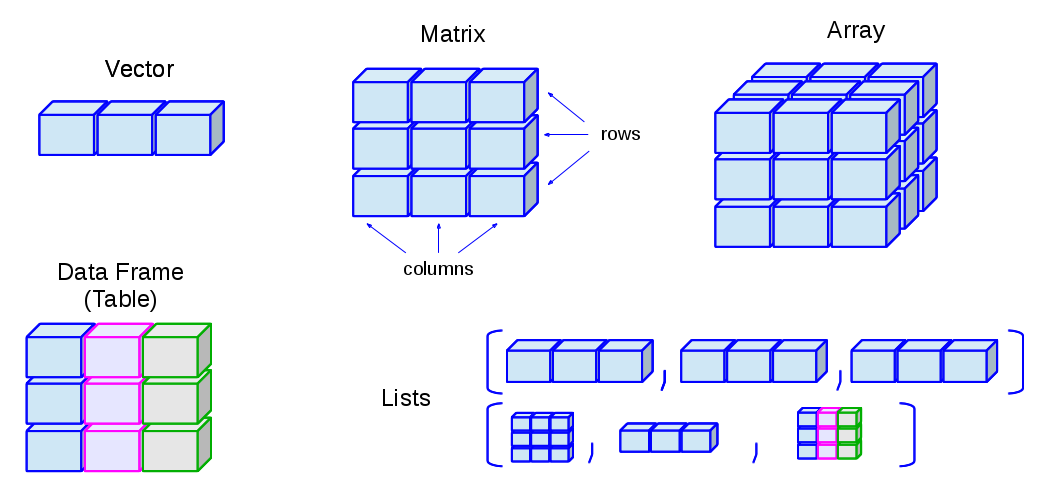
\includegraphics{./images/dataStructure.png}
\caption{}
\end{figure}

\subsection{Vectors}\label{vectors}

In R the simplest data structure is a vector. A vector is defined as an
ordered sequence of elements of the same kind.

A vector can be defined according to the data type it contains.
Therefore, there are:

\begin{itemize}
\tightlist
\item
  numeric vectors;
\item
  logical (or Boolean) vectors;
\item
  character (or string) vectors.
\end{itemize}

The most common method to define a vector is the \texttt{c()} function.

\begin{Shaded}
\begin{Highlighting}[]
\CommentTok{# Numeric vector}
\NormalTok{num <-}\StringTok{ }\KeywordTok{c}\NormalTok{(}\DecValTok{1}\NormalTok{, }\DecValTok{2}\NormalTok{, }\FloatTok{5.3}\NormalTok{, }\DecValTok{6}\NormalTok{, -}\DecValTok{2}\NormalTok{, }\DecValTok{4}\NormalTok{)}
\NormalTok{num}
\end{Highlighting}
\end{Shaded}

\begin{verbatim}
## [1]  1.0  2.0  5.3  6.0 -2.0  4.0
\end{verbatim}

\begin{Shaded}
\begin{Highlighting}[]
\CommentTok{# Character vector}
\NormalTok{char <-}\StringTok{ }\KeywordTok{c}\NormalTok{(}\StringTok{"one"}\NormalTok{, }\StringTok{"two"}\NormalTok{, }\StringTok{"three"}\NormalTok{)}
\NormalTok{char}
\end{Highlighting}
\end{Shaded}

\begin{verbatim}
## [1] "one"   "two"   "three"
\end{verbatim}

Logical vectors are often defined as the result of control actions on
numerical or character vectors.

\begin{Shaded}
\begin{Highlighting}[]
\CommentTok{# Logical vector}
\NormalTok{logic1 <-}\StringTok{ }\NormalTok{num >}\StringTok{ }\DecValTok{3}
\NormalTok{logic1}
\end{Highlighting}
\end{Shaded}

\begin{verbatim}
## [1] FALSE FALSE  TRUE  TRUE FALSE  TRUE
\end{verbatim}

Of course, a logical vector can be created using the \texttt{c()}
function.

\begin{Shaded}
\begin{Highlighting}[]
\CommentTok{# Logical vector}
\NormalTok{logic2 <-}\StringTok{ }\KeywordTok{c}\NormalTok{(}\OtherTok{TRUE}\NormalTok{, }\OtherTok{FALSE}\NormalTok{, }\OtherTok{TRUE}\NormalTok{)}
\NormalTok{logic2}
\end{Highlighting}
\end{Shaded}

\begin{verbatim}
## [1]  TRUE FALSE  TRUE
\end{verbatim}

If a vector mixes different data types, R will store it as a character
vector.

\begin{Shaded}
\begin{Highlighting}[]
\NormalTok{mixed <-}\StringTok{ }\KeywordTok{c}\NormalTok{(}\StringTok{"foo"}\NormalTok{, }\DecValTok{1}\NormalTok{, }\OtherTok{TRUE}\NormalTok{)}
\NormalTok{mixed}
\end{Highlighting}
\end{Shaded}

\begin{verbatim}
## [1] "foo"  "1"    "TRUE"
\end{verbatim}

The \texttt{c()} function can be used to create a vector combining
several vectors.

\begin{Shaded}
\begin{Highlighting}[]
\NormalTok{vec1 <-}\StringTok{ }\KeywordTok{c}\NormalTok{(}\DecValTok{11}\NormalTok{, }\DecValTok{12}\NormalTok{, }\DecValTok{13}\NormalTok{)}
\NormalTok{vec2 <-}\StringTok{ }\KeywordTok{c}\NormalTok{(}\DecValTok{21}\NormalTok{, }\DecValTok{22}\NormalTok{, }\DecValTok{23}\NormalTok{)}
\NormalTok{vec3 <-}\StringTok{ }\KeywordTok{c}\NormalTok{(}\DecValTok{31}\NormalTok{, }\DecValTok{32}\NormalTok{, }\DecValTok{33}\NormalTok{)}
\NormalTok{comb <-}\StringTok{ }\KeywordTok{c}\NormalTok{(vec1, vec2, vec3)}
\NormalTok{comb}
\end{Highlighting}
\end{Shaded}

\begin{verbatim}
## [1] 11 12 13 21 22 23 31 32 33
\end{verbatim}

A vector can be created using sequences. The easiest method is using the
operator \texttt{:}. The inputs of the operator \texttt{:} are the first
number on the left and the last number on the right. The vector will be
composed of numbers comprised between the first and the last number (by
one unit).

\begin{Shaded}
\begin{Highlighting}[]
\NormalTok{go <-}\StringTok{ }\DecValTok{1}\NormalTok{:}\DecValTok{20}
\NormalTok{go}
\end{Highlighting}
\end{Shaded}

\begin{verbatim}
##  [1]  1  2  3  4  5  6  7  8  9 10 11 12 13 14 15 16 17 18 19 20
\end{verbatim}

\begin{Shaded}
\begin{Highlighting}[]
\NormalTok{back <-}\StringTok{ }\DecValTok{20}\NormalTok{:}\DecValTok{1}
\NormalTok{back}
\end{Highlighting}
\end{Shaded}

\begin{verbatim}
##  [1] 20 19 18 17 16 15 14 13 12 11 10  9  8  7  6  5  4  3  2  1
\end{verbatim}

Other sequences can be created using the \texttt{seq()} function. The
parameters \texttt{from} and \texttt{to} of the \texttt{seq()} function
refer to the starting and end values of the sequence, respectively. The
parameter \texttt{by} indicates the number by which the sequence has to
be incremented. Alternatively, the \texttt{length.out} parameter refers
to the desired length of the sequence.

\begin{Shaded}
\begin{Highlighting}[]
\NormalTok{seqby <-}\StringTok{ }\KeywordTok{seq}\NormalTok{(}\DataTypeTok{from =} \DecValTok{1}\NormalTok{, }\DataTypeTok{to =} \DecValTok{5}\NormalTok{, }\DataTypeTok{by =} \FloatTok{0.5}\NormalTok{)}
\NormalTok{seqby}
\end{Highlighting}
\end{Shaded}

\begin{verbatim}
## [1] 1.0 1.5 2.0 2.5 3.0 3.5 4.0 4.5 5.0
\end{verbatim}

\begin{Shaded}
\begin{Highlighting}[]
\NormalTok{seqlength <-}\StringTok{ }\KeywordTok{seq}\NormalTok{(}\DataTypeTok{from =} \DecValTok{1}\NormalTok{, }\DataTypeTok{to =} \DecValTok{5}\NormalTok{, }\DataTypeTok{length.out =} \DecValTok{13}\NormalTok{) }
\NormalTok{seqlength}
\end{Highlighting}
\end{Shaded}

\begin{verbatim}
##  [1] 1.000000 1.333333 1.666667 2.000000 2.333333 2.666667 3.000000 3.333333 3.666667 4.000000 4.333333
## [12] 4.666667 5.000000
\end{verbatim}

Finally, vectors can be created with the \texttt{rep()} function which
repeats the elements of a vector. The first parameter of the
\texttt{rep()} function, \texttt{x}, is the value or vector to be
repeated and the second parameter, \texttt{times}, represents the number
of repetitions to be made. Alternatively, the \texttt{each} parameter
enables the repetition of each element of the vector as many times as
indicated by the number.

\begin{Shaded}
\begin{Highlighting}[]
\KeywordTok{rep}\NormalTok{(}\DataTypeTok{x =} \DecValTok{1} \NormalTok{, }\DataTypeTok{times =} \DecValTok{10}\NormalTok{)}
\end{Highlighting}
\end{Shaded}

\begin{verbatim}
##  [1] 1 1 1 1 1 1 1 1 1 1
\end{verbatim}

\begin{Shaded}
\begin{Highlighting}[]
\KeywordTok{rep}\NormalTok{(}\DataTypeTok{x =} \DecValTok{1}\NormalTok{:}\DecValTok{5}\NormalTok{, }\DataTypeTok{times =} \DecValTok{3}\NormalTok{)}
\end{Highlighting}
\end{Shaded}

\begin{verbatim}
##  [1] 1 2 3 4 5 1 2 3 4 5 1 2 3 4 5
\end{verbatim}

\begin{Shaded}
\begin{Highlighting}[]
\KeywordTok{rep}\NormalTok{(}\DataTypeTok{x =} \DecValTok{1}\NormalTok{:}\DecValTok{5} \NormalTok{, }\DataTypeTok{each =} \DecValTok{3}\NormalTok{)}
\end{Highlighting}
\end{Shaded}

\begin{verbatim}
##  [1] 1 1 1 2 2 2 3 3 3 4 4 4 5 5 5
\end{verbatim}

\begin{Shaded}
\begin{Highlighting}[]
\KeywordTok{rep}\NormalTok{(}\KeywordTok{c}\NormalTok{(}\StringTok{"ALI"}\NormalTok{, }\StringTok{"IPERLANDO"}\NormalTok{), }\DataTypeTok{times=}\DecValTok{4}\NormalTok{)}
\end{Highlighting}
\end{Shaded}

\begin{verbatim}
## [1] "ALI"       "IPERLANDO" "ALI"       "IPERLANDO" "ALI"       "IPERLANDO" "ALI"       "IPERLANDO"
\end{verbatim}

\begin{Shaded}
\begin{Highlighting}[]
\KeywordTok{rep}\NormalTok{(}\DataTypeTok{x =} \DecValTok{1}\NormalTok{:}\DecValTok{5} \NormalTok{, }\DataTypeTok{times =} \DecValTok{2} \NormalTok{, }\DataTypeTok{each =} \DecValTok{3}\NormalTok{)}
\end{Highlighting}
\end{Shaded}

\begin{verbatim}
##  [1] 1 1 1 2 2 2 3 3 3 4 4 4 5 5 5 1 1 1 2 2 2 3 3 3 4 4 4 5 5 5
\end{verbatim}

\begin{Shaded}
\begin{Highlighting}[]
\KeywordTok{rep}\NormalTok{(}\DataTypeTok{x =} \StringTok{"no"}\NormalTok{,  }\DataTypeTok{times =} \DecValTok{5}\NormalTok{)}
\end{Highlighting}
\end{Shaded}

\begin{verbatim}
## [1] "no" "no" "no" "no" "no"
\end{verbatim}

\begin{Shaded}
\begin{Highlighting}[]
\KeywordTok{rep}\NormalTok{(}\DataTypeTok{x =} \KeywordTok{c}\NormalTok{(}\StringTok{"a"}\NormalTok{, }\StringTok{"b"}\NormalTok{, }\StringTok{"c"}\NormalTok{), }\DataTypeTok{times =} \KeywordTok{c}\NormalTok{(}\DecValTok{3}\NormalTok{, }\DecValTok{2}\NormalTok{, }\DecValTok{1}\NormalTok{))}
\end{Highlighting}
\end{Shaded}

\begin{verbatim}
## [1] "a" "a" "a" "b" "b" "c"
\end{verbatim}

\begin{Shaded}
\begin{Highlighting}[]
\KeywordTok{rep}\NormalTok{(}\DataTypeTok{x =} \KeywordTok{c}\NormalTok{(}\StringTok{"a"}\NormalTok{, }\StringTok{"b"}\NormalTok{, }\StringTok{"c"}\NormalTok{), }\DataTypeTok{times =} \KeywordTok{rep}\NormalTok{(}\DecValTok{4}\NormalTok{,}\DecValTok{3}\NormalTok{))}
\end{Highlighting}
\end{Shaded}

\begin{verbatim}
##  [1] "a" "a" "a" "a" "b" "b" "b" "b" "c" "c" "c" "c"
\end{verbatim}

\begin{Shaded}
\begin{Highlighting}[]
\NormalTok{mydata <-}\StringTok{ }\KeywordTok{c}\NormalTok{(}\StringTok{"a"}\NormalTok{, }\StringTok{"b"}\NormalTok{, }\StringTok{"c"}\NormalTok{)}
\NormalTok{myrep <-}\StringTok{ }\KeywordTok{rep}\NormalTok{(}\DecValTok{4}\NormalTok{,}\DecValTok{3}\NormalTok{)}
\KeywordTok{rep}\NormalTok{(}\DataTypeTok{x =} \NormalTok{mydata, }\DataTypeTok{times =} \NormalTok{myrep)}
\end{Highlighting}
\end{Shaded}

\begin{verbatim}
##  [1] "a" "a" "a" "a" "b" "b" "b" "b" "c" "c" "c" "c"
\end{verbatim}

A subset of the vector \texttt{x} can be extracted with
\texttt{x{[}subscripts{]}}. The selection can be done in three ways.

\begin{enumerate}
\def\labelenumi{\arabic{enumi}.}
\tightlist
\item
  A vector of positive integers indicating the elements of the vector to
  be extracted.
\end{enumerate}

\begin{Shaded}
\begin{Highlighting}[]
\NormalTok{x <-}\StringTok{ }\KeywordTok{c}\NormalTok{(}\DecValTok{1}\NormalTok{, }\DecValTok{4}\NormalTok{, }\DecValTok{2}\NormalTok{, }\DecValTok{5}\NormalTok{, }\DecValTok{6}\NormalTok{, }\DecValTok{8}\NormalTok{, }\DecValTok{6}\NormalTok{, }\DecValTok{9}\NormalTok{, }\DecValTok{10}\NormalTok{)}
\NormalTok{x[}\DecValTok{3}\NormalTok{]}
\end{Highlighting}
\end{Shaded}

\begin{verbatim}
## [1] 2
\end{verbatim}

\begin{Shaded}
\begin{Highlighting}[]
\NormalTok{x[}\DecValTok{1}\NormalTok{:}\DecValTok{3}\NormalTok{]}
\end{Highlighting}
\end{Shaded}

\begin{verbatim}
## [1] 1 4 2
\end{verbatim}

\begin{Shaded}
\begin{Highlighting}[]
\NormalTok{x[}\KeywordTok{c}\NormalTok{(}\DecValTok{2}\NormalTok{,}\DecValTok{4}\NormalTok{)]}
\end{Highlighting}
\end{Shaded}

\begin{verbatim}
## [1] 4 5
\end{verbatim}

\begin{enumerate}
\def\labelenumi{\arabic{enumi}.}
\setcounter{enumi}{1}
\tightlist
\item
  A vector of negative integers indicating the elements which must not
  be extracted.
\end{enumerate}

\begin{Shaded}
\begin{Highlighting}[]
\NormalTok{x <-}\StringTok{ }\KeywordTok{c}\NormalTok{(}\DecValTok{1}\NormalTok{, }\DecValTok{4}\NormalTok{, }\DecValTok{2}\NormalTok{, }\DecValTok{5}\NormalTok{, }\DecValTok{6}\NormalTok{, }\DecValTok{8}\NormalTok{, }\DecValTok{6}\NormalTok{, }\DecValTok{9}\NormalTok{, }\DecValTok{10}\NormalTok{)}
\NormalTok{x[-}\DecValTok{2}\NormalTok{]}
\end{Highlighting}
\end{Shaded}

\begin{verbatim}
## [1]  1  2  5  6  8  6  9 10
\end{verbatim}

\begin{Shaded}
\begin{Highlighting}[]
\NormalTok{x[-}\KeywordTok{c}\NormalTok{(}\DecValTok{2}\NormalTok{, }\DecValTok{5}\NormalTok{, }\DecValTok{7}\NormalTok{)]}
\end{Highlighting}
\end{Shaded}

\begin{verbatim}
## [1]  1  2  5  8  9 10
\end{verbatim}

\begin{enumerate}
\def\labelenumi{\arabic{enumi}.}
\setcounter{enumi}{2}
\tightlist
\item
  A Boolean vector indicating the elements to be extracted
  (\texttt{TRUE}) or to be left (\texttt{FALSE}).
\end{enumerate}

\begin{Shaded}
\begin{Highlighting}[]
\NormalTok{x <-}\StringTok{ }\KeywordTok{c}\NormalTok{(}\DecValTok{1}\NormalTok{, }\DecValTok{4}\NormalTok{, }\DecValTok{2}\NormalTok{, }\DecValTok{5}\NormalTok{, }\DecValTok{6}\NormalTok{)}
\NormalTok{x[}\KeywordTok{c}\NormalTok{(}\OtherTok{TRUE}\NormalTok{, }\OtherTok{TRUE}\NormalTok{, }\OtherTok{FALSE}\NormalTok{, }\OtherTok{FALSE}\NormalTok{, }\OtherTok{TRUE}\NormalTok{)]}
\end{Highlighting}
\end{Shaded}

\begin{verbatim}
## [1] 1 4 6
\end{verbatim}

\begin{Shaded}
\begin{Highlighting}[]
\NormalTok{y <-}\StringTok{ }\KeywordTok{c}\NormalTok{(}\OtherTok{TRUE}\NormalTok{, }\OtherTok{TRUE}\NormalTok{, }\OtherTok{FALSE}\NormalTok{, }\OtherTok{FALSE}\NormalTok{, }\OtherTok{TRUE}\NormalTok{)}
\NormalTok{x[y]}
\end{Highlighting}
\end{Shaded}

\begin{verbatim}
## [1] 1 4 6
\end{verbatim}

\begin{Shaded}
\begin{Highlighting}[]
\NormalTok{x[!y]}
\end{Highlighting}
\end{Shaded}

\begin{verbatim}
## [1] 2 5
\end{verbatim}

The \texttt{!} symbol identifies the ``not'' logical operator. The
logical operator ``not'' reverses the logical value of a condition on
which it operates.

In this way elements satisfying a logical condition can be extracted.
Usually, the logical vectors are obtained as the result of logical
expressions.

\begin{Shaded}
\begin{Highlighting}[]
\NormalTok{x <-}\StringTok{ }\KeywordTok{c}\NormalTok{(}\DecValTok{1}\NormalTok{, }\DecValTok{4}\NormalTok{, }\DecValTok{2}\NormalTok{, }\DecValTok{5}\NormalTok{, }\DecValTok{6}\NormalTok{, }\DecValTok{8}\NormalTok{, }\DecValTok{6}\NormalTok{, }\DecValTok{9}\NormalTok{, }\DecValTok{10}\NormalTok{)}
\NormalTok{y <-}\StringTok{ }\NormalTok{x >}\StringTok{ }\DecValTok{5}
\NormalTok{x[y]}
\end{Highlighting}
\end{Shaded}

\begin{verbatim}
## [1]  6  8  6  9 10
\end{verbatim}

The logical expression can be defined inside the square brackets,
directly.

\begin{Shaded}
\begin{Highlighting}[]
\NormalTok{x[x >}\StringTok{ }\DecValTok{5}\NormalTok{]}
\end{Highlighting}
\end{Shaded}

\begin{verbatim}
## [1]  6  8  6  9 10
\end{verbatim}

The \texttt{\&} symbol identifies the ``and'' logical operator. The
``and'' logical operator compare two (or more) logical expression and
return TRUE if both are TRUE. The following example returns the
\texttt{x} values greater or equal than 2 but less or equal than 8.

\begin{Shaded}
\begin{Highlighting}[]
\NormalTok{x[x >=}\StringTok{ }\DecValTok{2} \NormalTok{&}\StringTok{ }\NormalTok{x <=}\StringTok{ }\DecValTok{8}\NormalTok{]}
\end{Highlighting}
\end{Shaded}

\begin{verbatim}
## [1] 4 2 5 6 8 6
\end{verbatim}

The \texttt{\textbar{}} symbol identifies the ``or'' logical operator.
The ``or'' logical operator compare two (or more) logical expression and
return TRUE if at least one is TRUE. The following example returns the
\texttt{x} values less than 2 or greater than 8.

\begin{Shaded}
\begin{Highlighting}[]
\NormalTok{x[x <}\StringTok{ }\DecValTok{2} \NormalTok{|}\StringTok{ }\NormalTok{x >}\StringTok{ }\DecValTok{8}\NormalTok{]}
\end{Highlighting}
\end{Shaded}

\begin{verbatim}
## [1]  1  9 10
\end{verbatim}

Extracting unique values contained in a vector can sometimes be useful.
This can be done with the \texttt{unique()} function.

\begin{Shaded}
\begin{Highlighting}[]
\NormalTok{x <-}\StringTok{ }\KeywordTok{c}\NormalTok{(}\DecValTok{1}\NormalTok{, }\DecValTok{2}\NormalTok{, }\DecValTok{1}\NormalTok{, }\DecValTok{1}\NormalTok{, }\DecValTok{2}\NormalTok{, }\DecValTok{3}\NormalTok{, }\DecValTok{3}\NormalTok{, }\DecValTok{2}\NormalTok{, }\DecValTok{1}\NormalTok{, }\DecValTok{2}\NormalTok{, }\DecValTok{2}\NormalTok{, }\DecValTok{3}\NormalTok{)}
\KeywordTok{unique}\NormalTok{(x)}
\end{Highlighting}
\end{Shaded}

\begin{verbatim}
## [1] 1 2 3
\end{verbatim}

\subsection{Matrices}\label{matrices}

Matrices are generalizations of vectors. Like vectors, matrices need to
contain elements of the same kind. This Paragraph introduces numeric
matrices.

A matrix can be created using the \texttt{matrix()} function.

\begin{Shaded}
\begin{Highlighting}[]
\KeywordTok{matrix}\NormalTok{(}\DecValTok{1}\NormalTok{:}\DecValTok{8}\NormalTok{, }\DataTypeTok{nrow =} \DecValTok{2}\NormalTok{, }\DataTypeTok{ncol =} \DecValTok{4}\NormalTok{)}
\end{Highlighting}
\end{Shaded}

\begin{verbatim}
##      [,1] [,2] [,3] [,4]
## [1,]    1    3    5    7
## [2,]    2    4    6    8
\end{verbatim}

By default, a matrix is filled by columns. The \texttt{byrow\ =\ TRUE}
argument of the \texttt{matrix()} function fills the matrix by rows.

\begin{Shaded}
\begin{Highlighting}[]
\KeywordTok{matrix}\NormalTok{(}\DecValTok{1}\NormalTok{:}\DecValTok{8}\NormalTok{, }\DataTypeTok{nrow =} \DecValTok{2}\NormalTok{, }\DataTypeTok{ncol =} \DecValTok{4}\NormalTok{, }\DataTypeTok{byrow =} \OtherTok{TRUE}\NormalTok{)}
\end{Highlighting}
\end{Shaded}

\begin{verbatim}
##      [,1] [,2] [,3] [,4]
## [1,]    1    2    3    4
## [2,]    5    6    7    8
\end{verbatim}

Alternatively, a matrix can be created by applying the \texttt{dim()}
function to a vector.

\begin{Shaded}
\begin{Highlighting}[]
\NormalTok{x <-}\StringTok{ }\DecValTok{1}\NormalTok{:}\DecValTok{8}
\NormalTok{x}
\end{Highlighting}
\end{Shaded}

\begin{verbatim}
## [1] 1 2 3 4 5 6 7 8
\end{verbatim}

\begin{Shaded}
\begin{Highlighting}[]
\KeywordTok{dim}\NormalTok{(x) <-}\StringTok{ }\KeywordTok{c}\NormalTok{(}\DecValTok{2}\NormalTok{, }\DecValTok{4}\NormalTok{)}
\NormalTok{x}
\end{Highlighting}
\end{Shaded}

\begin{verbatim}
##      [,1] [,2] [,3] [,4]
## [1,]    1    3    5    7
## [2,]    2    4    6    8
\end{verbatim}

Finally, a matrix can be created by joining two or more vectors, both as
column vectors (\texttt{cbind()} function) and row vectors
(\texttt{rbind()} function).

\begin{Shaded}
\begin{Highlighting}[]
\NormalTok{cmat <-}\StringTok{ }\KeywordTok{cbind}\NormalTok{(}\DecValTok{1}\NormalTok{:}\DecValTok{3}\NormalTok{, }\DecValTok{4}\NormalTok{:}\DecValTok{6}\NormalTok{, }\DecValTok{7}\NormalTok{:}\DecValTok{9}\NormalTok{)}
\NormalTok{cmat}
\end{Highlighting}
\end{Shaded}

\begin{verbatim}
##      [,1] [,2] [,3]
## [1,]    1    4    7
## [2,]    2    5    8
## [3,]    3    6    9
\end{verbatim}

\begin{Shaded}
\begin{Highlighting}[]
\NormalTok{rmat <-}\StringTok{ }\KeywordTok{rbind}\NormalTok{(}\DecValTok{1}\NormalTok{:}\DecValTok{3}\NormalTok{, }\DecValTok{4}\NormalTok{:}\DecValTok{6}\NormalTok{, }\DecValTok{7}\NormalTok{:}\DecValTok{9}\NormalTok{)}
\NormalTok{rmat}
\end{Highlighting}
\end{Shaded}

\begin{verbatim}
##      [,1] [,2] [,3]
## [1,]    1    2    3
## [2,]    4    5    6
## [3,]    7    8    9
\end{verbatim}

The \texttt{cbind()} and \texttt{rbind()} functions can be used to join
two (ore more) matrices or vectors and matrices.

\begin{Shaded}
\begin{Highlighting}[]
\KeywordTok{cbind}\NormalTok{(cmat, }\DecValTok{10}\NormalTok{:}\DecValTok{12}\NormalTok{)}
\end{Highlighting}
\end{Shaded}

\begin{verbatim}
##      [,1] [,2] [,3] [,4]
## [1,]    1    4    7   10
## [2,]    2    5    8   11
## [3,]    3    6    9   12
\end{verbatim}

\begin{Shaded}
\begin{Highlighting}[]
\KeywordTok{rbind}\NormalTok{(cmat, rmat, cmat)}
\end{Highlighting}
\end{Shaded}

\begin{verbatim}
##       [,1] [,2] [,3]
##  [1,]    1    4    7
##  [2,]    2    5    8
##  [3,]    3    6    9
##  [4,]    1    2    3
##  [5,]    4    5    6
##  [6,]    7    8    9
##  [7,]    1    4    7
##  [8,]    2    5    8
##  [9,]    3    6    9
\end{verbatim}

Like vectors, a subset of the matrix \texttt{x} can be extracted with
\texttt{x{[}subscripts{]}}. Subscripts can be:

\begin{enumerate}
\def\labelenumi{\arabic{enumi}.}
\tightlist
\item
  a set \texttt{{[}rows,\ cols{]}}, where \texttt{rows} is a vector of
  row numbers and \texttt{cols} is a vector of column numbers. Numbers
  are negative when they indicate a row or column to be excluded.
\item
  A number, a vector of numbers or a logical condition. In this case,
  the matrix is treated as if it were a single vector created by stacked
  matrix columns.
\end{enumerate}

\begin{Shaded}
\begin{Highlighting}[]
\NormalTok{x <-}\StringTok{ }\KeywordTok{matrix}\NormalTok{(}\DecValTok{1}\NormalTok{:}\DecValTok{24}\NormalTok{, }\DataTypeTok{nrow =} \DecValTok{4}\NormalTok{, }\DataTypeTok{ncol =} \DecValTok{6}\NormalTok{, }\DataTypeTok{byrow =} \OtherTok{TRUE}\NormalTok{)}
\NormalTok{x[}\DecValTok{1}\NormalTok{:}\DecValTok{2}\NormalTok{, ]}
\end{Highlighting}
\end{Shaded}

\begin{verbatim}
##      [,1] [,2] [,3] [,4] [,5] [,6]
## [1,]    1    2    3    4    5    6
## [2,]    7    8    9   10   11   12
\end{verbatim}

\begin{Shaded}
\begin{Highlighting}[]
\NormalTok{x[, }\KeywordTok{c}\NormalTok{(}\DecValTok{1}\NormalTok{, }\DecValTok{3}\NormalTok{, }\DecValTok{5}\NormalTok{)]}
\end{Highlighting}
\end{Shaded}

\begin{verbatim}
##      [,1] [,2] [,3]
## [1,]    1    3    5
## [2,]    7    9   11
## [3,]   13   15   17
## [4,]   19   21   23
\end{verbatim}

\begin{Shaded}
\begin{Highlighting}[]
\NormalTok{x[}\KeywordTok{c}\NormalTok{(}\DecValTok{1}\NormalTok{,}\DecValTok{3}\NormalTok{), }\KeywordTok{c}\NormalTok{(}\DecValTok{1}\NormalTok{, }\DecValTok{4}\NormalTok{)]}
\end{Highlighting}
\end{Shaded}

\begin{verbatim}
##      [,1] [,2]
## [1,]    1    4
## [2,]   13   16
\end{verbatim}

\begin{Shaded}
\begin{Highlighting}[]
\NormalTok{x[-}\DecValTok{1}\NormalTok{, ]}
\end{Highlighting}
\end{Shaded}

\begin{verbatim}
##      [,1] [,2] [,3] [,4] [,5] [,6]
## [1,]    7    8    9   10   11   12
## [2,]   13   14   15   16   17   18
## [3,]   19   20   21   22   23   24
\end{verbatim}

\begin{Shaded}
\begin{Highlighting}[]
\NormalTok{x[}\DecValTok{1}\NormalTok{:}\DecValTok{18}\NormalTok{]}
\end{Highlighting}
\end{Shaded}

\begin{verbatim}
##  [1]  1  7 13 19  2  8 14 20  3  9 15 21  4 10 16 22  5 11
\end{verbatim}

\begin{Shaded}
\begin{Highlighting}[]
\NormalTok{x[x >=}\StringTok{ }\DecValTok{3} \NormalTok{&}\StringTok{ }\NormalTok{x <}\StringTok{ }\DecValTok{12}\NormalTok{]}
\end{Highlighting}
\end{Shaded}

\begin{verbatim}
## [1]  7  8  3  9  4 10  5 11  6
\end{verbatim}

\subsection{Array}\label{array}

They are similar to matrices but they can be multi-dimensional (more
than two dimensions)

\begin{Shaded}
\begin{Highlighting}[]
\NormalTok{z <-}\StringTok{ }\KeywordTok{array}\NormalTok{(}\DecValTok{1}\NormalTok{:}\DecValTok{24}\NormalTok{, }\DataTypeTok{dim=}\KeywordTok{c}\NormalTok{(}\DecValTok{2}\NormalTok{,}\DecValTok{3}\NormalTok{,}\DecValTok{4}\NormalTok{))}
\NormalTok{z}
\end{Highlighting}
\end{Shaded}

\begin{verbatim}
## , , 1
## 
##      [,1] [,2] [,3]
## [1,]    1    3    5
## [2,]    2    4    6
## 
## , , 2
## 
##      [,1] [,2] [,3]
## [1,]    7    9   11
## [2,]    8   10   12
## 
## , , 3
## 
##      [,1] [,2] [,3]
## [1,]   13   15   17
## [2,]   14   16   18
## 
## , , 4
## 
##      [,1] [,2] [,3]
## [1,]   19   21   23
## [2,]   20   22   24
\end{verbatim}

\subsection{Lists}\label{lists}

A list is an ordered collection of objects. Each object is a component
of the list. Each element of the list can have a different structure. It
can be a list itself, a vector, a matrix, an array, a factor or a data
frame. A list allows you to gather a variety of (possibly unrelated)
objects under one name.

Lists are not usually created by users but are the result of statistical
procedures in R.

For example, in its simplest form, the \texttt{lsfit()} function
estimates a least-squares regression.

\begin{Shaded}
\begin{Highlighting}[]
\NormalTok{x <-}\StringTok{ }\DecValTok{1}\NormalTok{:}\DecValTok{5}
\NormalTok{y <-}\StringTok{ }\KeywordTok{c}\NormalTok{(-}\FloatTok{0.0921}\NormalTok{, }\FloatTok{0.4543}\NormalTok{, -}\FloatTok{0.1473}\NormalTok{, -}\FloatTok{0.0235}\NormalTok{, -}\FloatTok{0.3923}\NormalTok{)}
\NormalTok{out <-}\StringTok{ }\KeywordTok{lsfit}\NormalTok{(x, y)}
\NormalTok{out}
\end{Highlighting}
\end{Shaded}

\begin{verbatim}
## $coefficients
## Intercept         X 
##   0.28328  -0.10782 
## 
## $residuals
## [1] -0.26756  0.38666 -0.10712  0.12450 -0.13648
## 
## $intercept
## [1] TRUE
## 
## $qr
## $qt
## [1]  0.08984521 -0.34095678  0.05740271  0.42144605  0.29288939
## 
## $qr
##       Intercept          X
## [1,] -2.2360680 -6.7082039
## [2,]  0.4472136  3.1622777
## [3,]  0.4472136 -0.1954395
## [4,]  0.4472136 -0.5116673
## [5,]  0.4472136 -0.8278950
## 
## $qraux
## [1] 1.447214 1.120788
## 
## $rank
## [1] 2
## 
## $pivot
## [1] 1 2
## 
## $tol
## [1] 1e-07
## 
## attr(,"class")
## [1] "qr"
\end{verbatim}

The output of the function is a list made of four objects called
``coefficients'', ``residuals'', ``intercept'' e ``qr''. The first
element of the list is a vector with intercept and slope. The second
element is a vector with the residuals of the model. The third element
is a Boolean vector of length one indicating if the model contains the
intercept. The fourth element is a list containing the QR matrix
decomposition of the independent variables.

Even if rarely used, \texttt{list()} is the basic function to create a
list. Its arguments are the elements of the list.

\begin{Shaded}
\begin{Highlighting}[]
\NormalTok{my_list <-}\StringTok{ }\KeywordTok{list}\NormalTok{(}\DataTypeTok{vec =} \DecValTok{1}\NormalTok{:}\DecValTok{7}\NormalTok{, }\DataTypeTok{mat =} \KeywordTok{matrix}\NormalTok{(}\DecValTok{1}\NormalTok{:}\DecValTok{12}\NormalTok{, }\DataTypeTok{ncol =} \DecValTok{3}\NormalTok{),}
  \DataTypeTok{lis =} \KeywordTok{list}\NormalTok{(}\DataTypeTok{a =} \DecValTok{1}\NormalTok{, }\DataTypeTok{b =} \NormalTok{letters[}\DecValTok{1}\NormalTok{:}\DecValTok{4}\NormalTok{]))}
\NormalTok{my_list}
\end{Highlighting}
\end{Shaded}

\begin{verbatim}
## $vec
## [1] 1 2 3 4 5 6 7
## 
## $mat
##      [,1] [,2] [,3]
## [1,]    1    5    9
## [2,]    2    6   10
## [3,]    3    7   11
## [4,]    4    8   12
## 
## $lis
## $lis$a
## [1] 1
## 
## $lis$b
## [1] "a" "b" "c" "d"
\end{verbatim}

The elements of a list can be extracted in three different ways:

\begin{enumerate}
\def\labelenumi{\arabic{enumi}.}
\tightlist
\item
  with square brackets;
\item
  with double square brackets;
\item
  with the name of the object inside the list.
\end{enumerate}

In the first case, square brackets can be used to extract a list made of
one or more objects. As for vectors, the position of the elements to be
included or excluded ought to be specified.

\begin{Shaded}
\begin{Highlighting}[]
\NormalTok{my_list[}\DecValTok{1}\NormalTok{:}\DecValTok{2}\NormalTok{]}
\end{Highlighting}
\end{Shaded}

\begin{verbatim}
## $vec
## [1] 1 2 3 4 5 6 7
## 
## $mat
##      [,1] [,2] [,3]
## [1,]    1    5    9
## [2,]    2    6   10
## [3,]    3    7   11
## [4,]    4    8   12
\end{verbatim}

\begin{Shaded}
\begin{Highlighting}[]
\NormalTok{my_list[-}\DecValTok{3}\NormalTok{]}
\end{Highlighting}
\end{Shaded}

\begin{verbatim}
## $vec
## [1] 1 2 3 4 5 6 7
## 
## $mat
##      [,1] [,2] [,3]
## [1,]    1    5    9
## [2,]    2    6   10
## [3,]    3    7   11
## [4,]    4    8   12
\end{verbatim}

\begin{Shaded}
\begin{Highlighting}[]
\NormalTok{ml1 <-}\StringTok{ }\NormalTok{my_list[}\DecValTok{1}\NormalTok{]}
\NormalTok{ml1}
\end{Highlighting}
\end{Shaded}

\begin{verbatim}
## $vec
## [1] 1 2 3 4 5 6 7
\end{verbatim}

In the second case, double square brackets can be used to extract one
object (only) from the list.

\begin{Shaded}
\begin{Highlighting}[]
\NormalTok{ml2 <-}\StringTok{ }\NormalTok{my_list[[}\DecValTok{1}\NormalTok{]]}
\NormalTok{ml2}
\end{Highlighting}
\end{Shaded}

\begin{verbatim}
## [1] 1 2 3 4 5 6 7
\end{verbatim}

\begin{Shaded}
\begin{Highlighting}[]
\NormalTok{my_list[[}\DecValTok{2}\NormalTok{]]}
\end{Highlighting}
\end{Shaded}

\begin{verbatim}
##      [,1] [,2] [,3]
## [1,]    1    5    9
## [2,]    2    6   10
## [3,]    3    7   11
## [4,]    4    8   12
\end{verbatim}

\begin{Shaded}
\begin{Highlighting}[]
\NormalTok{my_list[[}\DecValTok{3}\NormalTok{]]}
\end{Highlighting}
\end{Shaded}

\begin{verbatim}
## $a
## [1] 1
## 
## $b
## [1] "a" "b" "c" "d"
\end{verbatim}

Please note the difference between \texttt{my\_list{[}1{]}} and
\texttt{my\_list{[}{[}1{]}{]}}. The first argument extracts a list with
only the first object contained in \texttt{my\_list}; in our case a
vector. On the other hand, the second argument extracts the vector,
which is the content of the first object of the list.

The third way enables the extraction of the content of an object in the
list. The use of the object position in the list, as for double square
brackets, is replaced by the use of the object name preceded by the
symbol \$.

\begin{Shaded}
\begin{Highlighting}[]
\NormalTok{my_list$vec}
\end{Highlighting}
\end{Shaded}

\begin{verbatim}
## [1] 1 2 3 4 5 6 7
\end{verbatim}

\begin{Shaded}
\begin{Highlighting}[]
\NormalTok{my_list$mat}
\end{Highlighting}
\end{Shaded}

\begin{verbatim}
##      [,1] [,2] [,3]
## [1,]    1    5    9
## [2,]    2    6   10
## [3,]    3    7   11
## [4,]    4    8   12
\end{verbatim}

\begin{Shaded}
\begin{Highlighting}[]
\NormalTok{my_list$lis}
\end{Highlighting}
\end{Shaded}

\begin{verbatim}
## $a
## [1] 1
## 
## $b
## [1] "a" "b" "c" "d"
\end{verbatim}

Indices for the selection can be combined to extract elements in an
object of the list using the above-mentioned methods.

\begin{Shaded}
\begin{Highlighting}[]
\NormalTok{my_list[[}\DecValTok{1}\NormalTok{]][}\DecValTok{1}\NormalTok{:}\DecValTok{3}\NormalTok{]}
\end{Highlighting}
\end{Shaded}

\begin{verbatim}
## [1] 1 2 3
\end{verbatim}

\begin{Shaded}
\begin{Highlighting}[]
\NormalTok{my_list$mat[}\DecValTok{3}\NormalTok{:}\DecValTok{4}\NormalTok{, }\KeywordTok{c}\NormalTok{(}\DecValTok{1}\NormalTok{, }\DecValTok{3}\NormalTok{)]}
\end{Highlighting}
\end{Shaded}

\begin{verbatim}
##      [,1] [,2]
## [1,]    3   11
## [2,]    4   12
\end{verbatim}

\begin{Shaded}
\begin{Highlighting}[]
\NormalTok{my_list$lis[}\DecValTok{1}\NormalTok{]}
\end{Highlighting}
\end{Shaded}

\begin{verbatim}
## $a
## [1] 1
\end{verbatim}

\begin{Shaded}
\begin{Highlighting}[]
\NormalTok{my_list$lis[[}\DecValTok{1}\NormalTok{]]}
\end{Highlighting}
\end{Shaded}

\begin{verbatim}
## [1] 1
\end{verbatim}

\begin{Shaded}
\begin{Highlighting}[]
\NormalTok{my_list$lis$a}
\end{Highlighting}
\end{Shaded}

\begin{verbatim}
## [1] 1
\end{verbatim}

\subsection{Factors}\label{factors}

A factor is a vector-like object used to specify a discrete
classification (grouping) of the components of other vectors of the same
length. R provides both \emph{ordered} and \emph{unordered} factors.

Factor variables are categorical variables that can be either numeric or
string variables. There are a number of advantages to converting
categorical variables to factor variables. Perhaps the most important
advantage is that they can be used in statistical modeling where they
will be implemented correctly, e.g., they will then be assigned the
correct number of degrees of freedom. Factor variables are also very
useful in many different types of graphics. Furthermore, storing string
variables as factor variables is a more efficient use of memory.

Vectors, matrices and lists contain numerical data, characters or logics
and are basic objects in R. Factors, on the other hand, are a more
complex structure, as they contain both the numerical data vector and
the labels associated with each level.

To create a factor variable the \texttt{factor()} function is used. The
only required argument is a vector of values which can be either string
or numeric. Optional arguments include the \texttt{levels} argument,
which determines the categories of the factor variable, and the default
is the sorted list of all the distinct values of the data vector. The
\texttt{labels} argument is another optional argument which is a vector
of values that will be the labels of the categories in the
\texttt{levels} argument. The \texttt{exclude} argument is also
optional; it defines which levels will be classified as NA in any output
using the factor variable.

\begin{Shaded}
\begin{Highlighting}[]
\NormalTok{grade <-}\StringTok{ }\KeywordTok{c}\NormalTok{(}\DecValTok{3}\NormalTok{, }\DecValTok{4}\NormalTok{, }\DecValTok{2}\NormalTok{, }\DecValTok{2}\NormalTok{, }\DecValTok{4}\NormalTok{, }\DecValTok{1}\NormalTok{, }\DecValTok{1}\NormalTok{, }\DecValTok{4}\NormalTok{, }\DecValTok{2}\NormalTok{, }\DecValTok{2}\NormalTok{)}
\KeywordTok{factor}\NormalTok{(grade)  }
\end{Highlighting}
\end{Shaded}

\begin{verbatim}
##  [1] 3 4 2 2 4 1 1 4 2 2
## Levels: 1 2 3 4
\end{verbatim}

\begin{Shaded}
\begin{Highlighting}[]
\NormalTok{gender <-}\StringTok{ }\KeywordTok{c}\NormalTok{(}\KeywordTok{rep}\NormalTok{(}\StringTok{"male"}\NormalTok{, }\DecValTok{3}\NormalTok{), }\KeywordTok{rep}\NormalTok{(}\StringTok{"female"}\NormalTok{, }\DecValTok{4}\NormalTok{))}
\NormalTok{gender <-}\StringTok{ }\KeywordTok{factor}\NormalTok{(gender, }\DataTypeTok{levels=}\KeywordTok{c}\NormalTok{(}\StringTok{"male"}\NormalTok{, }\StringTok{"female"}\NormalTok{, }\StringTok{"trans"}\NormalTok{))}
\NormalTok{gender}
\end{Highlighting}
\end{Shaded}

\begin{verbatim}
## [1] male   male   male   female female female female
## Levels: male female trans
\end{verbatim}

Once a vector has been defined, it is always possible to modify the
labels of the vector's levels. This can be done with the
\texttt{levels()} function.

\begin{Shaded}
\begin{Highlighting}[]
\NormalTok{size <-}\StringTok{ }\KeywordTok{factor}\NormalTok{(}\KeywordTok{c}\NormalTok{(}\DecValTok{2}\NormalTok{, }\DecValTok{3}\NormalTok{, }\DecValTok{1}\NormalTok{, }\DecValTok{1}\NormalTok{, }\DecValTok{1}\NormalTok{, }\DecValTok{2}\NormalTok{, }\DecValTok{3}\NormalTok{, }\DecValTok{3}\NormalTok{), }\DataTypeTok{levels =} \KeywordTok{c}\NormalTok{(}\DecValTok{1}\NormalTok{, }\DecValTok{2}\NormalTok{, }\DecValTok{3}\NormalTok{),}
  \DataTypeTok{labels =} \KeywordTok{c}\NormalTok{(}\StringTok{"small"}\NormalTok{, }\StringTok{"medium"}\NormalTok{, }\StringTok{"large"}\NormalTok{))}
\KeywordTok{levels}\NormalTok{(size)}
\end{Highlighting}
\end{Shaded}

\begin{verbatim}
## [1] "small"  "medium" "large"
\end{verbatim}

\begin{Shaded}
\begin{Highlighting}[]
\KeywordTok{levels}\NormalTok{(size) <-}\StringTok{ }\KeywordTok{c}\NormalTok{(}\StringTok{"S"}\NormalTok{, }\StringTok{"M"}\NormalTok{, }\StringTok{"L"}\NormalTok{)}
\NormalTok{size}
\end{Highlighting}
\end{Shaded}

\begin{verbatim}
## [1] M L S S S M L L
## Levels: S M L
\end{verbatim}

The \texttt{order} parameter of the \texttt{factor()} function creates a
factor with ordered levels.

\begin{Shaded}
\begin{Highlighting}[]
\NormalTok{mark <-}\StringTok{ }\KeywordTok{sample}\NormalTok{(}\KeywordTok{c}\NormalTok{(}\StringTok{"D"}\NormalTok{, }\StringTok{"C"}\NormalTok{, }\StringTok{"B"}\NormalTok{, }\StringTok{"A"}\NormalTok{), }\DecValTok{12}\NormalTok{, }\DataTypeTok{replace =} \NormalTok{T)}
\NormalTok{mark1 <-}\StringTok{ }\KeywordTok{factor}\NormalTok{(mark)}
\NormalTok{mark2 <-}\StringTok{ }\KeywordTok{factor}\NormalTok{(mark, }\DataTypeTok{levels =} \KeywordTok{c}\NormalTok{(}\StringTok{"D"}\NormalTok{, }\StringTok{"C"}\NormalTok{, }\StringTok{"B"}\NormalTok{, }\StringTok{"A"}\NormalTok{), }\DataTypeTok{order =} \NormalTok{T)}
\NormalTok{mark1}
\end{Highlighting}
\end{Shaded}

\begin{verbatim}
##  [1] B D D A B D C A A D B D
## Levels: A B C D
\end{verbatim}

\begin{Shaded}
\begin{Highlighting}[]
\NormalTok{mark2}
\end{Highlighting}
\end{Shaded}

\begin{verbatim}
##  [1] B D D A B D C A A D B D
## Levels: D < C < B < A
\end{verbatim}

The \texttt{as.numeric()} and \texttt{as.character()} functions
transform a factor into a numeric vector or into a vector whose elements
are the levels' labels.

\begin{Shaded}
\begin{Highlighting}[]
\KeywordTok{as.numeric}\NormalTok{(size)}
\end{Highlighting}
\end{Shaded}

\begin{verbatim}
## [1] 2 3 1 1 1 2 3 3
\end{verbatim}

\begin{Shaded}
\begin{Highlighting}[]
\KeywordTok{as.character}\NormalTok{(size)}
\end{Highlighting}
\end{Shaded}

\begin{verbatim}
## [1] "M" "L" "S" "S" "S" "M" "L" "L"
\end{verbatim}

The elements of a factor can be extracted in the same way as the
elements of a vector. The logic conditions on the elements of a factor
are referred to the factor's levels which can be obtained with
the\texttt{levels()} function.

\begin{Shaded}
\begin{Highlighting}[]
\NormalTok{size <-}\StringTok{ }\KeywordTok{factor}\NormalTok{(}\KeywordTok{c}\NormalTok{(}\DecValTok{2}\NormalTok{, }\DecValTok{3}\NormalTok{, }\DecValTok{1}\NormalTok{, }\DecValTok{1}\NormalTok{, }\DecValTok{1}\NormalTok{, }\DecValTok{2}\NormalTok{, }\DecValTok{3}\NormalTok{, }\DecValTok{3}\NormalTok{), }\DataTypeTok{levels =} \KeywordTok{c}\NormalTok{(}\DecValTok{1}\NormalTok{, }\DecValTok{2}\NormalTok{, }\DecValTok{3}\NormalTok{),}
  \DataTypeTok{labels =} \KeywordTok{c}\NormalTok{(}\StringTok{"small"}\NormalTok{, }\StringTok{"medium"}\NormalTok{, }\StringTok{"large"}\NormalTok{))}
\NormalTok{size}
\end{Highlighting}
\end{Shaded}

\begin{verbatim}
## [1] medium large  small  small  small  medium large  large 
## Levels: small medium large
\end{verbatim}

\begin{Shaded}
\begin{Highlighting}[]
\NormalTok{size[}\DecValTok{1}\NormalTok{:}\DecValTok{5}\NormalTok{]}
\end{Highlighting}
\end{Shaded}

\begin{verbatim}
## [1] medium large  small  small  small 
## Levels: small medium large
\end{verbatim}

\begin{Shaded}
\begin{Highlighting}[]
\NormalTok{size[-}\DecValTok{4}\NormalTok{]}
\end{Highlighting}
\end{Shaded}

\begin{verbatim}
## [1] medium large  small  small  medium large  large 
## Levels: small medium large
\end{verbatim}

\begin{Shaded}
\begin{Highlighting}[]
\KeywordTok{levels}\NormalTok{(size)}
\end{Highlighting}
\end{Shaded}

\begin{verbatim}
## [1] "small"  "medium" "large"
\end{verbatim}

\begin{Shaded}
\begin{Highlighting}[]
\NormalTok{size[size ==}\StringTok{ "medium"} \NormalTok{|}\StringTok{ }\NormalTok{size ==}\StringTok{ "large"}\NormalTok{]}
\end{Highlighting}
\end{Shaded}

\begin{verbatim}
## [1] medium large  medium large  large 
## Levels: small medium large
\end{verbatim}

\subsection{Data Frames}\label{data-frames}

A data frame in R can be thought of as:

\begin{itemize}
\tightlist
\item
  a generalization of a matrix;
\item
  a list of particular kind.
\end{itemize}

In the first case a data frame can be thought of as a matrix whose
columns can be both factors and vectors of the same length but
(possibly) of different types (numeric, character, Boolean).

In the second case, the data frame is a list completely made of either
vectors (of any kind) or factors, all with the same length.

From a formal point of view, data frames are not a new type of objects.
They are objects of list type and data frame class. From a practical
point of view, a data frame is a very well-know structure in statistics.
Its different kinds of information are organized in columns, whereas
rows represent different types of observational units.

Furthermore, data imported in R from external sources, such as text
files, Excel files or databases, is saved in R as data frame-like
objects.

To sum up, unless we have specific needs, data frames in R are the ideal
tool for data filing and management.

Data frames are usually imported from external sources but the creation
of a data frame object in R might sometimes be needed. The most
widespread method to define a data frame is the \texttt{data.frame()}
function. Its inputs are a series of vectors or factors of the same
length. The generated object is made of as many columns as input
elements.

\begin{Shaded}
\begin{Highlighting}[]
\NormalTok{name <-}\StringTok{ }\KeywordTok{c}\NormalTok{(}\StringTok{"James"}\NormalTok{, }\StringTok{"Stevie"}\NormalTok{, }\StringTok{"Otis"}\NormalTok{, }\StringTok{"Bob"}\NormalTok{, }\StringTok{"Levon"}\NormalTok{, }\StringTok{"Patti"}\NormalTok{, }\StringTok{"Karen"}\NormalTok{)}
\NormalTok{height <-}\StringTok{ }\KeywordTok{c}\NormalTok{(}\DecValTok{180}\NormalTok{, }\DecValTok{170}\NormalTok{, }\DecValTok{175}\NormalTok{, }\DecValTok{190}\NormalTok{, }\DecValTok{168}\NormalTok{, }\DecValTok{160}\NormalTok{, }\DecValTok{165}\NormalTok{)}
\NormalTok{gender <-}\StringTok{ }\KeywordTok{factor}\NormalTok{(}\KeywordTok{c}\NormalTok{(}\StringTok{"M"}\NormalTok{, }\StringTok{"M"}\NormalTok{, }\StringTok{"M"}\NormalTok{, }\StringTok{"M"}\NormalTok{, }\StringTok{"M"}\NormalTok{, }\StringTok{"F"}\NormalTok{, }\StringTok{"F"}\NormalTok{))}
\NormalTok{df <-}\StringTok{ }\KeywordTok{data.frame}\NormalTok{(name, height, gender, }\DataTypeTok{stringsAsFactors =} \OtherTok{FALSE}\NormalTok{)}
\NormalTok{df}
\end{Highlighting}
\end{Shaded}

\begin{verbatim}
##     name height gender
## 1  James    180      M
## 2 Stevie    170      M
## 3   Otis    175      M
## 4    Bob    190      M
## 5  Levon    168      M
## 6  Patti    160      F
## 7  Karen    165      F
\end{verbatim}

Alternatively, the vectors composing the data frame can be defined
inside the \texttt{data.frame()} function itself.

\begin{Shaded}
\begin{Highlighting}[]
\NormalTok{df <-}\StringTok{ }\KeywordTok{data.frame}\NormalTok{(}
  \DataTypeTok{height =} \KeywordTok{c}\NormalTok{(}\DecValTok{180}\NormalTok{, }\DecValTok{170}\NormalTok{, }\DecValTok{175}\NormalTok{, }\DecValTok{190}\NormalTok{, }\DecValTok{168}\NormalTok{, }\DecValTok{160}\NormalTok{, }\DecValTok{165}\NormalTok{),}
  \DataTypeTok{name =} \KeywordTok{c}\NormalTok{(}\StringTok{"James"}\NormalTok{, }\StringTok{"Stevie"}\NormalTok{, }\StringTok{"Otis"}\NormalTok{, }\StringTok{"Bob"}\NormalTok{, }\StringTok{"Levon"}\NormalTok{, }\StringTok{"Patti"}\NormalTok{, }\StringTok{"Karen"}\NormalTok{),}
  \DataTypeTok{gender =} \KeywordTok{factor}\NormalTok{(}\KeywordTok{c}\NormalTok{(}\StringTok{"M"}\NormalTok{, }\StringTok{"M"}\NormalTok{, }\StringTok{"M"}\NormalTok{, }\StringTok{"M"}\NormalTok{, }\StringTok{"M"}\NormalTok{, }\StringTok{"F"}\NormalTok{, }\StringTok{"F"}\NormalTok{)),}
  \DataTypeTok{stringsAsFactors =} \OtherTok{FALSE}
\NormalTok{)}
\NormalTok{df}
\end{Highlighting}
\end{Shaded}

\begin{verbatim}
##   height   name gender
## 1    180  James      M
## 2    170 Stevie      M
## 3    175   Otis      M
## 4    190    Bob      M
## 5    168  Levon      M
## 6    160  Patti      F
## 7    165  Karen      F
\end{verbatim}

The management of character vectors in R requires a detailed
explanation. By default, numeric vectors become part of data frames as
such, whereas character vectors are transformed into factors whose
levels correspond to the vector's unique values.

This behaviour is surely effective when character vectors represent
categorical variables with a definite number of modes, such as education
qualification or job.

A character vector can also represent a set of strings which are not
necessarily referable to a definite number of modes (e.g.~person's
proper names) or to numerous and/or unique modes (e.g.~Italian
municipalities are about 8,000 and have different names). In this case
R's behaviour becomes a disturbing factor because it tends to transform
variables of a different nature into factors.

Unfortunately, there is not an optimal solution to this problem. Much
depends on the most used types of variables dealt with by a single user.

This behaviour is managed by the \texttt{stringsAsFactors} logical
parameter.

As already mentioned, the default setting is
\texttt{stringsAsFactors\ =\ TRUE} which tells R to transform character
vectors into factors inside a data frame;
\texttt{stringsAsFactors\ =\ FALSE} does not change character vectors.
This parameter can be set both in ``local'' option with the
\texttt{stringsAsFactors} parameter inside the \texttt{data.frame()}
function and in ``global'' option with \texttt{stringsAsFactors} inside
the \texttt{options()} function. Clearly, the ``global'' option of the
\texttt{stringsAsFactors} lasts for the whole session of work but can be
locally modified in any moment in a single call to a function.

There are several ways to extract a subset from a data frame. Data
management is not among topics of this introductory manual. Like
matrices, data can be extracted using \texttt{x{[}subscripts{]}} where
subscripts is a set \texttt{{[}rows,\ cols{]}}, where \texttt{rows} is a
vector of row numbers and \texttt{cols} is a vector of column numbers.
Numbers are negative when they indicate a row or column to be excluded.

The following code chunk shows how to extract the first, the third and
the seventh row from the \texttt{df} dataframe.

\begin{Shaded}
\begin{Highlighting}[]
\NormalTok{df[}\KeywordTok{c}\NormalTok{(}\DecValTok{1}\NormalTok{, }\DecValTok{3}\NormalTok{, }\DecValTok{7}\NormalTok{), ]}
\end{Highlighting}
\end{Shaded}

\begin{verbatim}
##   height  name gender
## 1    180 James      M
## 3    175  Otis      M
## 7    165 Karen      F
\end{verbatim}

The code below shows how to extract the first and the second column from
the \texttt{df} dataframe.

\begin{Shaded}
\begin{Highlighting}[]
\NormalTok{df[, }\KeywordTok{c}\NormalTok{(}\DecValTok{1}\NormalTok{, }\DecValTok{2}\NormalTok{)]}
\end{Highlighting}
\end{Shaded}

\begin{verbatim}
##   height   name
## 1    180  James
## 2    170 Stevie
## 3    175   Otis
## 4    190    Bob
## 5    168  Levon
## 6    160  Patti
## 7    165  Karen
\end{verbatim}

Like lists, data can be extracted using \texttt{x\$column} where column
is the column name.

\begin{Shaded}
\begin{Highlighting}[]
\NormalTok{df$height}
\end{Highlighting}
\end{Shaded}

\begin{verbatim}
## [1] 180 170 175 190 168 160 165
\end{verbatim}

\begin{Shaded}
\begin{Highlighting}[]
\KeywordTok{is.vector}\NormalTok{(df$height)}
\end{Highlighting}
\end{Shaded}

\begin{verbatim}
## [1] TRUE
\end{verbatim}

The above code returns a vector. To get a data frame, the
\texttt{data.frame()} function can be used.

\begin{Shaded}
\begin{Highlighting}[]
\KeywordTok{data.frame}\NormalTok{(}\DataTypeTok{height =} \NormalTok{df$height)}
\end{Highlighting}
\end{Shaded}

\begin{verbatim}
##   height
## 1    180
## 2    170
## 3    175
## 4    190
## 5    168
## 6    160
## 7    165
\end{verbatim}

\begin{Shaded}
\begin{Highlighting}[]
\KeywordTok{data.frame}\NormalTok{(}\DataTypeTok{height =} \NormalTok{df$height, }\DataTypeTok{name =} \NormalTok{df$name)}
\end{Highlighting}
\end{Shaded}

\begin{verbatim}
##   height   name
## 1    180  James
## 2    170 Stevie
## 3    175   Otis
## 4    190    Bob
## 5    168  Levon
## 6    160  Patti
## 7    165  Karen
\end{verbatim}

The \texttt{dim()} function can be used to know the number of rows and
of columns of a data frame. The same information can be obtained using
\texttt{nrow()} and \texttt{ncol()} functions, respectively.

\begin{Shaded}
\begin{Highlighting}[]
\KeywordTok{dim}\NormalTok{(df)}
\end{Highlighting}
\end{Shaded}

\begin{verbatim}
## [1] 7 3
\end{verbatim}

\begin{Shaded}
\begin{Highlighting}[]
\KeywordTok{nrow}\NormalTok{(df)}
\end{Highlighting}
\end{Shaded}

\begin{verbatim}
## [1] 7
\end{verbatim}

\begin{Shaded}
\begin{Highlighting}[]
\KeywordTok{ncol}\NormalTok{(df)}
\end{Highlighting}
\end{Shaded}

\begin{verbatim}
## [1] 3
\end{verbatim}

The \texttt{str()} function returns the structure of a dataframe. For
each variable (column), it shows: the name, the type (numeric,
character, factor etc.) and first elements.

\begin{Shaded}
\begin{Highlighting}[]
\NormalTok{df}
\end{Highlighting}
\end{Shaded}

\begin{verbatim}
##   height   name gender
## 1    180  James      M
## 2    170 Stevie      M
## 3    175   Otis      M
## 4    190    Bob      M
## 5    168  Levon      M
## 6    160  Patti      F
## 7    165  Karen      F
\end{verbatim}

\begin{Shaded}
\begin{Highlighting}[]
\KeywordTok{str}\NormalTok{(df)}
\end{Highlighting}
\end{Shaded}

\begin{verbatim}
## 'data.frame':    7 obs. of  3 variables:
##  $ height: num  180 170 175 190 168 160 165
##  $ name  : chr  "James" "Stevie" "Otis" "Bob" ...
##  $ gender: Factor w/ 2 levels "F","M": 2 2 2 2 2 1 1
\end{verbatim}

The \texttt{head()} function show the first rows of a data frame. Its
use is particularly convenient when data sets are long. \texttt{iris} is
a built in R data set. It contains the measurements in centimeters of
the variables sepal length and width and petal length and width,
respectively, for 50 flowers from each of 3 species of iris.

\begin{Shaded}
\begin{Highlighting}[]
\KeywordTok{nrow}\NormalTok{(iris)}
\end{Highlighting}
\end{Shaded}

\begin{verbatim}
## [1] 150
\end{verbatim}

\begin{Shaded}
\begin{Highlighting}[]
\KeywordTok{head}\NormalTok{(iris)}
\end{Highlighting}
\end{Shaded}

\begin{verbatim}
##   Sepal.Length Sepal.Width Petal.Length Petal.Width Species
## 1          5.1         3.5          1.4         0.2  setosa
## 2          4.9         3.0          1.4         0.2  setosa
## 3          4.7         3.2          1.3         0.2  setosa
## 4          4.6         3.1          1.5         0.2  setosa
## 5          5.0         3.6          1.4         0.2  setosa
## 6          5.4         3.9          1.7         0.4  setosa
\end{verbatim}

\subsection{Missing Values, Null Objects and
Infinite}\label{missing-values-null-objects-and-infinite}

In R missing values are represented by the symbol \texttt{NA} (Not
Available).

\begin{Shaded}
\begin{Highlighting}[]
\NormalTok{x <-}\StringTok{ }\KeywordTok{c}\NormalTok{(}\DecValTok{4}\NormalTok{, }\DecValTok{1}\NormalTok{, }\StringTok{"a"}\NormalTok{)}
\NormalTok{y <-}\StringTok{ }\KeywordTok{as.integer}\NormalTok{(x)}
\end{Highlighting}
\end{Shaded}

\begin{verbatim}
## Warning: NAs introduced by coercion
\end{verbatim}

\begin{Shaded}
\begin{Highlighting}[]
\NormalTok{y}
\end{Highlighting}
\end{Shaded}

\begin{verbatim}
## [1]  4  1 NA
\end{verbatim}

The above chunk create a vector \texttt{x}. The vector contains three
values: 4, 1 and the character string ``a''. Then, elements of the
vector are transformed into integer values.

The character string ``a'' cannot be transformed, so a \texttt{NA} value
is returned.

To check if data is missing, the function \texttt{is.na()} can be used.

\begin{Shaded}
\begin{Highlighting}[]
\KeywordTok{is.na}\NormalTok{(y)}
\end{Highlighting}
\end{Shaded}

\begin{verbatim}
## [1] FALSE FALSE  TRUE
\end{verbatim}

The \texttt{NaN} symbol (Not a Number) represents a missing value
obtained as a result of an impossible numerical operation. \texttt{NaN}
can be detected with the function is.nan.

\begin{Shaded}
\begin{Highlighting}[]
\KeywordTok{log}\NormalTok{(-}\DecValTok{1}\NormalTok{)}
\end{Highlighting}
\end{Shaded}

\begin{verbatim}
## Warning in log(-1): NaNs produced
\end{verbatim}

\begin{verbatim}
## [1] NaN
\end{verbatim}

\begin{Shaded}
\begin{Highlighting}[]
\KeywordTok{sqrt}\NormalTok{(-}\DecValTok{4}\NormalTok{)}
\end{Highlighting}
\end{Shaded}

\begin{verbatim}
## Warning in sqrt(-4): NaNs produced
\end{verbatim}

\begin{verbatim}
## [1] NaN
\end{verbatim}

\begin{Shaded}
\begin{Highlighting}[]
\NormalTok{x <-}\StringTok{ }\KeywordTok{log}\NormalTok{(}\KeywordTok{c}\NormalTok{(-}\DecValTok{1}\NormalTok{, }\DecValTok{1}\NormalTok{, }\DecValTok{2}\NormalTok{))}
\end{Highlighting}
\end{Shaded}

\begin{verbatim}
## Warning in log(c(-1, 1, 2)): NaNs produced
\end{verbatim}

\begin{Shaded}
\begin{Highlighting}[]
\NormalTok{x}
\end{Highlighting}
\end{Shaded}

\begin{verbatim}
## [1]       NaN 0.0000000 0.6931472
\end{verbatim}

\begin{Shaded}
\begin{Highlighting}[]
\KeywordTok{is.nan}\NormalTok{(x)}
\end{Highlighting}
\end{Shaded}

\begin{verbatim}
## [1]  TRUE FALSE FALSE
\end{verbatim}

The \texttt{NULL} symbol represents the null object in R. \texttt{NULL}
is often returned by expressions and functions whose value is undefined.
The \texttt{is.null()} function returns \texttt{TRUE} if its argument is
\texttt{NULL} and FALSE otherwise.

\begin{Shaded}
\begin{Highlighting}[]
\NormalTok{x <-}\StringTok{ }\KeywordTok{c}\NormalTok{()}
\NormalTok{x}
\end{Highlighting}
\end{Shaded}

\begin{verbatim}
## NULL
\end{verbatim}

\begin{Shaded}
\begin{Highlighting}[]
\KeywordTok{is.null}\NormalTok{(x)}
\end{Highlighting}
\end{Shaded}

\begin{verbatim}
## [1] TRUE
\end{verbatim}

Infinite values are represented by the \texttt{+Inf} and \texttt{-Inf}
symbols in R.

\begin{Shaded}
\begin{Highlighting}[]
\KeywordTok{log}\NormalTok{(}\DecValTok{0}\NormalTok{)}
\end{Highlighting}
\end{Shaded}

\begin{verbatim}
## [1] -Inf
\end{verbatim}

In the above example, R calculates the limit of the function \(log(x)\)
as \(x\) approaches zero.

\section{Function Object}\label{function-object}

Functions are one of the most important objects in R as when working
with R we all make constant use of functions.

A function is characterised by an input and an output. The input of the
function, i.e.~the set of the arguments, can be either null or made of
one or more R objects. The output of the function can be either null or
a single R object. If the function has to return more than one object,
the objects are to be inserted in a list.

Let us see some examples:

The function \texttt{ls()} doesn't require any input and returns an
output.

\begin{Shaded}
\begin{Highlighting}[]
\KeywordTok{ls}\NormalTok{()}
\end{Highlighting}
\end{Shaded}

\begin{verbatim}
##  [1] "back"      "char"      "cmat"      "comb"      "df"        "gender"    "go"        "grade"    
##  [9] "height"    "logic1"    "logic2"    "mark"      "mark1"     "mark2"     "mixed"     "ml1"      
## [17] "ml2"       "mydata"    "my_list"   "myrep"     "name"      "num"       "out"       "rmat"     
## [25] "seqby"     "seqlength" "size"      "vec1"      "vec2"      "vec3"      "x"         "y"        
## [33] "z"
\end{verbatim}

The function \texttt{rm()} requires an input and doesn't return an
output.

\begin{Shaded}
\begin{Highlighting}[]
\NormalTok{foo <-}\StringTok{ }\DecValTok{3}
\KeywordTok{rm}\NormalTok{(foo)}
\end{Highlighting}
\end{Shaded}

Usually, functions require an input and returns an output.

\begin{Shaded}
\begin{Highlighting}[]
\KeywordTok{sum}\NormalTok{(}\DecValTok{1}\NormalTok{:}\DecValTok{10}\NormalTok{)}
\end{Highlighting}
\end{Shaded}

\begin{verbatim}
## [1] 55
\end{verbatim}

It is advisable to use the help command of each function to understand
not only the arguments which can be used as function inputs, but also
the output:

\begin{Shaded}
\begin{Highlighting}[]
\KeywordTok{help}\NormalTok{(read.table)}
\end{Highlighting}
\end{Shaded}

or

\begin{Shaded}
\begin{Highlighting}[]
\NormalTok{?read.table}
\end{Highlighting}
\end{Shaded}

Let us deeply explore function structure.

\subsection{Function structure}\label{function-structure}

We can create and assign functions to a variable name as we do with any
other object:

\begin{Shaded}
\begin{Highlighting}[]
\NormalTok{f <-}\StringTok{ }\NormalTok{function(x, }\DataTypeTok{y =} \DecValTok{0}\NormalTok{) \{}
  \NormalTok{z <-}\StringTok{ }\NormalTok{x +}\StringTok{ }\NormalTok{y}
  \NormalTok{z}
\NormalTok{\}}
\end{Highlighting}
\end{Shaded}

Eventually, we can delete any function with the usual call to
\texttt{rm()} or \texttt{remove()}

Function structure is made up by three basic components:

\begin{itemize}
\tightlist
\item
  a formal arguments list
\item
  a body
\item
  an environment.
\end{itemize}

\begin{Shaded}
\begin{Highlighting}[]
\KeywordTok{formals}\NormalTok{(f)}
\end{Highlighting}
\end{Shaded}

\begin{verbatim}
## $x
## 
## 
## $y
## [1] 0
\end{verbatim}

\begin{Shaded}
\begin{Highlighting}[]
\KeywordTok{body}\NormalTok{(f)}
\end{Highlighting}
\end{Shaded}

\begin{verbatim}
## {
##     z <- x + y
##     z
## }
\end{verbatim}

\begin{Shaded}
\begin{Highlighting}[]
\KeywordTok{environment}\NormalTok{(f)}
\end{Highlighting}
\end{Shaded}

\begin{verbatim}
## <environment: R_GlobalEnv>
\end{verbatim}

\subsubsection{Formals}\label{formals}

Formals are the formal arguments of a function.

When we call a function, formals arguments can be specified by position
or by name and we can mix positional matching with matching by name so
that the following are equivalent:

\begin{Shaded}
\begin{Highlighting}[]
\KeywordTok{mean}\NormalTok{(}\DataTypeTok{x =} \DecValTok{1}\NormalTok{:}\DecValTok{5}\NormalTok{, }\DataTypeTok{trim =} \FloatTok{0.1}\NormalTok{)}
\end{Highlighting}
\end{Shaded}

\begin{verbatim}
## [1] 3
\end{verbatim}

\begin{Shaded}
\begin{Highlighting}[]
\KeywordTok{mean}\NormalTok{(}\DecValTok{1}\NormalTok{:}\DecValTok{5}\NormalTok{, }\DataTypeTok{trim =} \FloatTok{0.1}\NormalTok{)}
\end{Highlighting}
\end{Shaded}

\begin{verbatim}
## [1] 3
\end{verbatim}

\begin{Shaded}
\begin{Highlighting}[]
\KeywordTok{mean}\NormalTok{(}\DataTypeTok{x =} \DecValTok{1}\NormalTok{:}\DecValTok{5}\NormalTok{, }\FloatTok{0.1}\NormalTok{)}
\end{Highlighting}
\end{Shaded}

\begin{verbatim}
## [1] 3
\end{verbatim}

\begin{Shaded}
\begin{Highlighting}[]
\KeywordTok{mean}\NormalTok{(}\DecValTok{1}\NormalTok{:}\DecValTok{5}\NormalTok{, }\FloatTok{0.1}\NormalTok{)}
\end{Highlighting}
\end{Shaded}

\begin{verbatim}
## [1] 3
\end{verbatim}

\begin{Shaded}
\begin{Highlighting}[]
\KeywordTok{mean}\NormalTok{(}\DataTypeTok{trim =} \FloatTok{0.1}\NormalTok{, }\DataTypeTok{x =} \DecValTok{1}\NormalTok{:}\DecValTok{5}\NormalTok{)}
\end{Highlighting}
\end{Shaded}

\begin{verbatim}
## [1] 3
\end{verbatim}

Along with position and name, we can also specify formals by partial
matching so that:

\begin{Shaded}
\begin{Highlighting}[]
\KeywordTok{mean}\NormalTok{(}\DecValTok{1}\NormalTok{:}\DecValTok{5}\NormalTok{, }\DataTypeTok{tr =} \FloatTok{0.1}\NormalTok{)}
\end{Highlighting}
\end{Shaded}

\begin{verbatim}
## [1] 3
\end{verbatim}

\begin{Shaded}
\begin{Highlighting}[]
\KeywordTok{mean}\NormalTok{(}\DataTypeTok{tr =} \FloatTok{0.1}\NormalTok{, }\DataTypeTok{x =} \DecValTok{1}\NormalTok{:}\DecValTok{5}\NormalTok{)}
\end{Highlighting}
\end{Shaded}

\begin{verbatim}
## [1] 3
\end{verbatim}

would work anyway.

Functions formals may also have the construct
\texttt{symbol\ =\ default}, that unless differently specified, forces
any argument to be used with its default value.

Specifically, function \texttt{mean()} also have a third argument
\texttt{na.rm} that defaults to \texttt{FALSE} and, as a result passing
vectors with \texttt{NA} values to \texttt{mean()} returns \texttt{NA}

\begin{Shaded}
\begin{Highlighting}[]
\KeywordTok{mean}\NormalTok{(}\KeywordTok{c}\NormalTok{(}\DecValTok{1}\NormalTok{, }\DecValTok{2}\NormalTok{, }\OtherTok{NA}\NormalTok{))}
\end{Highlighting}
\end{Shaded}

\begin{verbatim}
## [1] NA
\end{verbatim}

While, by specifying \texttt{na.rm=TRUE} we get the mean of all non
missing elements of vector \texttt{x}.

\begin{Shaded}
\begin{Highlighting}[]
\KeywordTok{mean}\NormalTok{(}\KeywordTok{c}\NormalTok{(}\DecValTok{1}\NormalTok{, }\DecValTok{2}\NormalTok{, }\OtherTok{NA}\NormalTok{), }\DataTypeTok{na.rm =} \OtherTok{TRUE}\NormalTok{)}
\end{Highlighting}
\end{Shaded}

\begin{verbatim}
## [1] 1.5
\end{verbatim}

The order \texttt{R} uses for matching formals against value is:

\begin{enumerate}
\def\labelenumi{\arabic{enumi}.}
\tightlist
\item
  Check for exact match for a named argument
\item
  Check for a partial match
\item
  Check for a positional match
\end{enumerate}

\subsubsection{Body of a function}\label{body-of-a-function}

The body of a function is a parsed R statement. In practice, this
implies that the body of a function needs to be correct from a formal
point of view but no evaluation of the body of a function occurred yet.

As a result, this function would return an error:

\begin{Shaded}
\begin{Highlighting}[]
\NormalTok{wrong <-}\StringTok{ }\NormalTok{function(x) \{x =\}}
\end{Highlighting}
\end{Shaded}

as its body is not a correct \texttt{R} statement.

While this function:

\begin{Shaded}
\begin{Highlighting}[]
\NormalTok{right <-}\StringTok{ }\NormalTok{function(x)\{x+h\}}
\end{Highlighting}
\end{Shaded}

is accepted by \texttt{R} as is formally correct even thought, except
under specific circumstances, will always return an error:

\begin{Shaded}
\begin{Highlighting}[]
\KeywordTok{right}\NormalTok{(}\DataTypeTok{x =} \DecValTok{2}\NormalTok{)}
\end{Highlighting}
\end{Shaded}

\begin{verbatim}
## Error in right(x = 2): object 'h' not found
\end{verbatim}

The body of a function, is usually a collection of statements in braces
but it can be a single statement, a symbol or even a constant.

\subsubsection{Environment of a
function}\label{environment-of-a-function}

Environments are a fundamental concept in R and their knowledge is
essential for advanced programming.

Environments have the following fundamental concepts:

\begin{itemize}
\item
  The environment of a function is the environment that was active at
  the time that the function was created. Generally, for user defined
  function, the Global environment:

\begin{Shaded}
\begin{Highlighting}[]
\NormalTok{f <-}\StringTok{ }\NormalTok{function(x)\{x}\DecValTok{+1}\NormalTok{\}}
\KeywordTok{environment}\NormalTok{(f)}
\end{Highlighting}
\end{Shaded}

\begin{verbatim}
## <environment: R_GlobalEnv>
\end{verbatim}

  or, when a function is defined within a package, the environment
  associated to that package:

\begin{Shaded}
\begin{Highlighting}[]
\KeywordTok{environment}\NormalTok{(mean)}
\end{Highlighting}
\end{Shaded}

\begin{verbatim}
## <environment: namespace:base>
\end{verbatim}
\item
  Objects defined within a function, exists in the environment of the
  function itself.

\begin{Shaded}
\begin{Highlighting}[]
\NormalTok{f <-}\StringTok{ }\NormalTok{function(x)\{x}\DecValTok{+1}\NormalTok{\}}
\NormalTok{x}
\end{Highlighting}
\end{Shaded}

\begin{verbatim}
## NULL
\end{verbatim}
\end{itemize}

\subsection{Function Examples}\label{function-examples}

There are lots of function types, let us see some examples.

\subsubsection{Mathematical Functions}\label{mathematical-functions}

The names of the basic functions and mathematical operators in R follow
the standards of programming languages. In this paragraph the functions
and operators enabling basic mathematical operations to be performed
will be dealt with. R can also be used to perform more complex
calculations, such as matrix operations or calculations with complex
numbers.

Functions are usually applied to one or more vectors. In this case,
operations are performed on each element of each vector. Vectors have to
be the same length.

\begin{Shaded}
\begin{Highlighting}[]
\NormalTok{x <-}\StringTok{ }\DecValTok{1}\NormalTok{:}\DecValTok{10}
\NormalTok{y <-}\StringTok{ }\DecValTok{11}\NormalTok{:}\DecValTok{20}
\NormalTok{z <-}\StringTok{ }\NormalTok{-}\DecValTok{4}\NormalTok{:}\DecValTok{5}
\NormalTok{x +}\StringTok{ }\NormalTok{y +}\StringTok{ }\NormalTok{z}
\end{Highlighting}
\end{Shaded}

\begin{verbatim}
##  [1]  8 11 14 17 20 23 26 29 32 35
\end{verbatim}

\begin{Shaded}
\begin{Highlighting}[]
\KeywordTok{exp}\NormalTok{(x)}
\end{Highlighting}
\end{Shaded}

\begin{verbatim}
##  [1]     2.718282     7.389056    20.085537    54.598150   148.413159   403.428793  1096.633158  2980.957987
##  [9]  8103.083928 22026.465795
\end{verbatim}

\begin{Shaded}
\begin{Highlighting}[]
\KeywordTok{log}\NormalTok{(z)}
\end{Highlighting}
\end{Shaded}

\begin{verbatim}
## Warning in log(z): NaNs produced
\end{verbatim}

\begin{verbatim}
##  [1]       NaN       NaN       NaN       NaN      -Inf 0.0000000 0.6931472 1.0986123 1.3862944 1.6094379
\end{verbatim}

\begin{Shaded}
\begin{Highlighting}[]
\KeywordTok{abs}\NormalTok{(z)}
\end{Highlighting}
\end{Shaded}

\begin{verbatim}
##  [1] 4 3 2 1 0 1 2 3 4 5
\end{verbatim}

\begin{Shaded}
\begin{Highlighting}[]
\KeywordTok{sqrt}\NormalTok{(x)}
\end{Highlighting}
\end{Shaded}

\begin{verbatim}
##  [1] 1.000000 1.414214 1.732051 2.000000 2.236068 2.449490 2.645751 2.828427 3.000000 3.162278
\end{verbatim}

The \texttt{sum()} function calculates the sum of all the elements of a
vector.

\begin{Shaded}
\begin{Highlighting}[]
\KeywordTok{sum}\NormalTok{(x)}
\end{Highlighting}
\end{Shaded}

\begin{verbatim}
## [1] 55
\end{verbatim}

The \texttt{floor}, \texttt{ceiling}, \texttt{trunc} and \texttt{round}
functions can be used to round a number. \texttt{floor()} returns a
numeric vector containing the largest integers not greater than the
corresponding input elements. \texttt{ceiling()} returns a numeric
vector containing the smallest integers not less than the corresponding
input elements. \texttt{trunc()} returns a numeric vector containing the
integers formed by truncating the input values toward 0.
\texttt{round()} rounds the values in its first argument to the
specified number of decimal places (default 0).

\begin{Shaded}
\begin{Highlighting}[]
\KeywordTok{floor}\NormalTok{(}\FloatTok{3.14}\NormalTok{)}
\end{Highlighting}
\end{Shaded}

\begin{verbatim}
## [1] 3
\end{verbatim}

\begin{Shaded}
\begin{Highlighting}[]
\KeywordTok{floor}\NormalTok{(}\FloatTok{3.67}\NormalTok{)}
\end{Highlighting}
\end{Shaded}

\begin{verbatim}
## [1] 3
\end{verbatim}

\begin{Shaded}
\begin{Highlighting}[]
\KeywordTok{ceiling}\NormalTok{(}\FloatTok{3.14}\NormalTok{)}
\end{Highlighting}
\end{Shaded}

\begin{verbatim}
## [1] 4
\end{verbatim}

\begin{Shaded}
\begin{Highlighting}[]
\KeywordTok{ceiling}\NormalTok{(}\FloatTok{3.67}\NormalTok{)}
\end{Highlighting}
\end{Shaded}

\begin{verbatim}
## [1] 4
\end{verbatim}

\begin{Shaded}
\begin{Highlighting}[]
\KeywordTok{trunc}\NormalTok{(}\FloatTok{3.14}\NormalTok{)}
\end{Highlighting}
\end{Shaded}

\begin{verbatim}
## [1] 3
\end{verbatim}

\begin{Shaded}
\begin{Highlighting}[]
\KeywordTok{trunc}\NormalTok{(}\FloatTok{3.67}\NormalTok{)}
\end{Highlighting}
\end{Shaded}

\begin{verbatim}
## [1] 3
\end{verbatim}

\begin{Shaded}
\begin{Highlighting}[]
\KeywordTok{round}\NormalTok{(}\FloatTok{3.14}\NormalTok{, }\DataTypeTok{digits =} \DecValTok{1}\NormalTok{)}
\end{Highlighting}
\end{Shaded}

\begin{verbatim}
## [1] 3.1
\end{verbatim}

\begin{Shaded}
\begin{Highlighting}[]
\KeywordTok{round}\NormalTok{(}\FloatTok{3.19}\NormalTok{, }\DataTypeTok{digits =} \DecValTok{1}\NormalTok{)}
\end{Highlighting}
\end{Shaded}

\begin{verbatim}
## [1] 3.2
\end{verbatim}

\subsubsection{Probabilistic Functions}\label{probabilistic-functions}

Probabilistic functions in R fall into four categories:

\begin{enumerate}
\def\labelenumi{\arabic{enumi}.}
\tightlist
\item
  \texttt{r*} functions for generating random numbers,
\item
  \texttt{d*} functions for calculating the value of the density
  function in a point,
\item
  \texttt{p*} functions for calculating the cumulative distribution
  function,
\item
  \texttt{q*} functions for calculating quantiles.
\end{enumerate}

The asterisk indicates the distribution which is used: \texttt{norm} for
normal distribution, \texttt{t} for Student's t-distribution,
\texttt{binom} for binomial distribution, \texttt{gamma} distribution,
\texttt{beta} distribution, \texttt{weibull} distribution, etc. R
integrates numerous statistical distributions. The list of all the
probability distributions included in the base R can be obtained by
typing \texttt{help(Distributions)}. Other probability distributions
become available when loading additional packages.

The following functions:

\begin{Shaded}
\begin{Highlighting}[]
\KeywordTok{rnorm}\NormalTok{(}\DataTypeTok{n =} \DecValTok{10}\NormalTok{)}
\end{Highlighting}
\end{Shaded}

\begin{verbatim}
##  [1]  0.03671286  1.44157390 -2.54593783  1.20381478  0.17470718  0.71825907  0.90201773 -0.81875316
##  [9]  0.41442748 -0.23316441
\end{verbatim}

\begin{Shaded}
\begin{Highlighting}[]
\KeywordTok{rnorm}\NormalTok{(}\DataTypeTok{n =} \DecValTok{20}\NormalTok{, }\DataTypeTok{mean =} \DecValTok{3}\NormalTok{, }\DataTypeTok{sd =} \DecValTok{5}\NormalTok{)}
\end{Highlighting}
\end{Shaded}

\begin{verbatim}
##  [1]  8.1161315  4.1175142  0.4305539 -3.2560182 10.1279865  0.5123030  2.4498182 10.0185880  0.4435542
## [10]  5.3219403  1.9810591 -1.0541618  2.5490966  3.7378717 -0.3524744  6.4293541  3.2363052  4.5638334
## [19]  3.9127530  3.0003167
\end{verbatim}

\begin{Shaded}
\begin{Highlighting}[]
\KeywordTok{rbinom}\NormalTok{(}\DataTypeTok{n =} \DecValTok{50}\NormalTok{, }\DataTypeTok{size =} \DecValTok{20}\NormalTok{, }\DataTypeTok{prob =} \FloatTok{0.8}\NormalTok{)}
\end{Highlighting}
\end{Shaded}

\begin{verbatim}
##  [1] 16 17 15 16 18 15 17 19 15 13 16 17 14 18 16 15 15 18 18 16 17 16 16 18 16 17 17 14 17 17 15 15 15 17
## [35] 17 18 16 16 15 16 17 18 16 16 16 13 17 11 14 16
\end{verbatim}

\begin{Shaded}
\begin{Highlighting}[]
\KeywordTok{rweibull}\NormalTok{(}\DataTypeTok{n =} \DecValTok{30}\NormalTok{, }\DataTypeTok{shape =} \DecValTok{5}\NormalTok{, }\DataTypeTok{scale =} \DecValTok{3}\NormalTok{)}
\end{Highlighting}
\end{Shaded}

\begin{verbatim}
##  [1] 2.982094 2.011687 1.794671 3.147264 2.388938 2.320514 2.494149 3.053366 1.220845 2.529022 1.919187
## [12] 3.067260 3.259476 1.747864 2.957188 2.141522 3.313209 3.085932 3.017064 3.369909 3.382658 2.365779
## [23] 2.828647 2.393660 2.943538 2.191707 2.649564 3.673390 2.700337 2.580711
\end{verbatim}

generate, respectively:

\begin{itemize}
\tightlist
\item
  10 pseudorandom values from a normal distribution with parameters (0,
  1);
\item
  20 pseudorandom values from a normal distribution with parameters (3,
  5);
\item
  50 pseudorandom values from a binomial distribution with \(n = 20\)
  and \(\pi = 0.8\);
\item
  50 pseudorandom values from a Weibull distribution with parameters (5,
  3).
\end{itemize}

The following functions:

\begin{Shaded}
\begin{Highlighting}[]
\KeywordTok{dbinom}\NormalTok{(}\DataTypeTok{x =} \DecValTok{20}\NormalTok{, }\DataTypeTok{size =} \DecValTok{20}\NormalTok{, }\DataTypeTok{prob =} \FloatTok{0.8}\NormalTok{)}
\end{Highlighting}
\end{Shaded}

\begin{verbatim}
## [1] 0.01152922
\end{verbatim}

\begin{Shaded}
\begin{Highlighting}[]
\KeywordTok{dnorm}\NormalTok{(}\DataTypeTok{x =} \NormalTok{-}\DecValTok{5}\NormalTok{:}\DecValTok{5}\NormalTok{, }\DataTypeTok{mean =} \DecValTok{0}\NormalTok{, }\DataTypeTok{sd =} \DecValTok{1}\NormalTok{)}
\end{Highlighting}
\end{Shaded}

\begin{verbatim}
##  [1] 1.486720e-06 1.338302e-04 4.431848e-03 5.399097e-02 2.419707e-01 3.989423e-01 2.419707e-01 5.399097e-02
##  [9] 4.431848e-03 1.338302e-04 1.486720e-06
\end{verbatim}

calculate, respectively:

\begin{itemize}
\tightlist
\item
  the probability that \texttt{x} is equal to 20, if \texttt{x} is
  distributed as a binomial distribution with \(n = 20\) and
  \(\pi = 0.8\);
\item
  thee values of the density function of a standard normal for integer
  values comprised between -5 and 5. As expected, the highest value is
  obtained with 0.
\end{itemize}

The following functions:

\begin{Shaded}
\begin{Highlighting}[]
\KeywordTok{pnorm}\NormalTok{(}\DataTypeTok{q =} \DecValTok{0}\NormalTok{, }\DataTypeTok{mean =} \DecValTok{0}\NormalTok{, }\DataTypeTok{sd =} \DecValTok{1}\NormalTok{)}
\end{Highlighting}
\end{Shaded}

\begin{verbatim}
## [1] 0.5
\end{verbatim}

\begin{Shaded}
\begin{Highlighting}[]
\KeywordTok{pbinom}\NormalTok{(}\DataTypeTok{q =} \DecValTok{20}\NormalTok{, }\DataTypeTok{size =} \DecValTok{20}\NormalTok{, }\DataTypeTok{prob =} \FloatTok{0.8}\NormalTok{)}
\end{Highlighting}
\end{Shaded}

\begin{verbatim}
## [1] 1
\end{verbatim}

calculate, respectively:

\begin{itemize}
\tightlist
\item
  the value of the cumulative distribution function of a standard normal
  distribution at zero; as expected the result is 0.5.
\item
  the value of a cumulative distribution function of a binomial
  distribution with parameters \(n = 20\) and \(\pi = 0.8\) at 20; as
  expected, the result is 1.
\end{itemize}

The following functions:

\begin{Shaded}
\begin{Highlighting}[]
\KeywordTok{qnorm}\NormalTok{(}\DataTypeTok{p =} \FloatTok{0.5}\NormalTok{, }\DataTypeTok{mean =} \DecValTok{0}\NormalTok{, }\DataTypeTok{sd =} \DecValTok{1}\NormalTok{)}
\end{Highlighting}
\end{Shaded}

\begin{verbatim}
## [1] 0
\end{verbatim}

\begin{Shaded}
\begin{Highlighting}[]
\KeywordTok{qbinom}\NormalTok{(}\DataTypeTok{p =} \FloatTok{0.5}\NormalTok{, }\DataTypeTok{size =} \DecValTok{20}\NormalTok{, }\DataTypeTok{prob =} \FloatTok{0.8}\NormalTok{)}
\end{Highlighting}
\end{Shaded}

\begin{verbatim}
## [1] 16
\end{verbatim}

calculate, respectively:

\begin{itemize}
\tightlist
\item
  the quantile with which a 0.5 probability on the left is obtained in a
  standard normal distribution;
\item
  The quantile with which a 0.5 probability on the left is obtained in a
  binomial distribution with parameters \(n = 20\) and \(\pi = 0.8\).
\end{itemize}

\subsubsection{Statistical Functions}\label{statistical-functions}

Any kind of statistical analysis can be performed in R thanks to the
built-in functions of the base version or the numerous additional
packages. The functions enabling the calculation of the main descriptive
statistical analyses are explained below.

The \texttt{mean()}, \texttt{median()}, \texttt{sd()} and \texttt{var()}
functions are used to calculate the mean, the median, the sample
standard deviation and the sample variance of a numeric vector.

\begin{Shaded}
\begin{Highlighting}[]
\NormalTok{x <-}\StringTok{ }\NormalTok{mtcars$mpg}
\KeywordTok{mean}\NormalTok{(x)}
\end{Highlighting}
\end{Shaded}

\begin{verbatim}
## [1] 20.09062
\end{verbatim}

\begin{Shaded}
\begin{Highlighting}[]
\KeywordTok{median}\NormalTok{(x)}
\end{Highlighting}
\end{Shaded}

\begin{verbatim}
## [1] 19.2
\end{verbatim}

\begin{Shaded}
\begin{Highlighting}[]
\KeywordTok{sd}\NormalTok{(x)  }
\end{Highlighting}
\end{Shaded}

\begin{verbatim}
## [1] 6.026948
\end{verbatim}

\begin{Shaded}
\begin{Highlighting}[]
\KeywordTok{var}\NormalTok{(x)}
\end{Highlighting}
\end{Shaded}

\begin{verbatim}
## [1] 36.3241
\end{verbatim}

The \texttt{quantile()} function calculates one or more quantiles.

\begin{Shaded}
\begin{Highlighting}[]
\KeywordTok{quantile}\NormalTok{(x, .}\DecValTok{9}\NormalTok{) }
\end{Highlighting}
\end{Shaded}

\begin{verbatim}
##   90% 
## 30.09
\end{verbatim}

\begin{Shaded}
\begin{Highlighting}[]
\KeywordTok{quantile}\NormalTok{(x, }\KeywordTok{c}\NormalTok{(.}\DecValTok{3}\NormalTok{, .}\DecValTok{84}\NormalTok{))}
\end{Highlighting}
\end{Shaded}

\begin{verbatim}
##    30%    84% 
## 15.980 26.052
\end{verbatim}

\begin{Shaded}
\begin{Highlighting}[]
\KeywordTok{quantile}\NormalTok{(x, }\KeywordTok{c}\NormalTok{(.}\DecValTok{25}\NormalTok{, .}\DecValTok{50}\NormalTok{, .}\DecValTok{75}\NormalTok{))}
\end{Highlighting}
\end{Shaded}

\begin{verbatim}
##    25%    50%    75% 
## 15.425 19.200 22.800
\end{verbatim}

The \texttt{min()} and \texttt{max()} functions return the minimum and
maximum value respectively.

\begin{Shaded}
\begin{Highlighting}[]
\KeywordTok{min}\NormalTok{(x)}
\end{Highlighting}
\end{Shaded}

\begin{verbatim}
## [1] 10.4
\end{verbatim}

\begin{Shaded}
\begin{Highlighting}[]
\KeywordTok{max}\NormalTok{(x)}
\end{Highlighting}
\end{Shaded}

\begin{verbatim}
## [1] 33.9
\end{verbatim}

The \texttt{summary()} generic function applied to a numeric vector
returns minimum, maximum, quartiles and arithmetic mean.

\begin{Shaded}
\begin{Highlighting}[]
\KeywordTok{summary}\NormalTok{(x)}
\end{Highlighting}
\end{Shaded}

\begin{verbatim}
##    Min. 1st Qu.  Median    Mean 3rd Qu.    Max. 
##   10.40   15.42   19.20   20.09   22.80   33.90
\end{verbatim}

Correlation and covariance can be calculated with the \texttt{cor()} and
\texttt{cov()} functions, respectively.

\begin{Shaded}
\begin{Highlighting}[]
\NormalTok{data <-}\StringTok{ }\NormalTok{mtcars[, }\KeywordTok{c}\NormalTok{(}\DecValTok{1}\NormalTok{, }\DecValTok{3}\NormalTok{, }\DecValTok{4}\NormalTok{, }\DecValTok{5}\NormalTok{, }\DecValTok{6}\NormalTok{)]}
\KeywordTok{cor}\NormalTok{(data)}
\end{Highlighting}
\end{Shaded}

\begin{verbatim}
##             mpg       disp         hp       drat         wt
## mpg   1.0000000 -0.8475514 -0.7761684  0.6811719 -0.8676594
## disp -0.8475514  1.0000000  0.7909486 -0.7102139  0.8879799
## hp   -0.7761684  0.7909486  1.0000000 -0.4487591  0.6587479
## drat  0.6811719 -0.7102139 -0.4487591  1.0000000 -0.7124406
## wt   -0.8676594  0.8879799  0.6587479 -0.7124406  1.0000000
\end{verbatim}

\begin{Shaded}
\begin{Highlighting}[]
\KeywordTok{cov}\NormalTok{(data)}
\end{Highlighting}
\end{Shaded}

\begin{verbatim}
##              mpg        disp         hp        drat          wt
## mpg    36.324103  -633.09721 -320.73206   2.1950635  -5.1166847
## disp -633.097208 15360.79983 6721.15867 -47.0640192 107.6842040
## hp   -320.732056  6721.15867 4700.86694 -16.4511089  44.1926613
## drat    2.195064   -47.06402  -16.45111   0.2858814  -0.3727207
## wt     -5.116685   107.68420   44.19266  -0.3727207   0.9573790
\end{verbatim}

\chapter{Introduction to Data Import and
Export}\label{introduction-to-data-import-and-export}

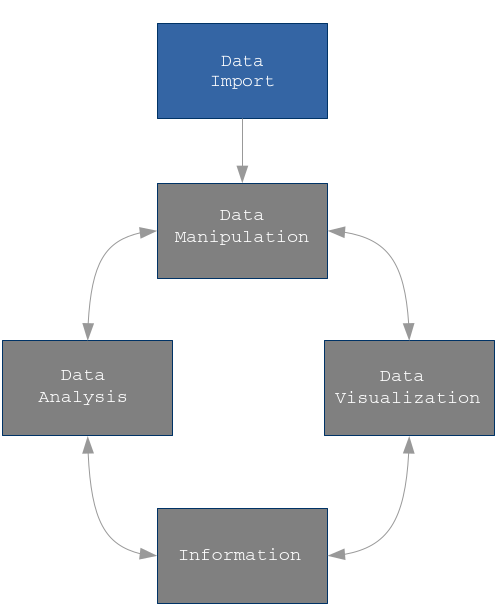
\includegraphics[width=2.94in]{images/flow-robj}

In the following chapters we will explore data import and export methods
for:

\begin{itemize}
\tightlist
\item
  Text files
\item
  Microsoft Excel files
\item
  Databases
\item
  R data files
\end{itemize}

\section{Text Files}\label{text-files}


\includegraphics[width=5.52in]{images/import-text-2}

\subsection{Data Import}\label{data-import}

The \texttt{read.table()} function imports a text file (ASCII) with a
table structure where each row represents a case.

A full path can be provided, but it must be modified by each user,
otherwise it fails:

\begin{Shaded}
\begin{Highlighting}[]
\NormalTok{df <-}\StringTok{ }\KeywordTok{read.table}\NormalTok{(}\StringTok{"C:/Users/UserName/Documents/data/tennis.txt"}\NormalTok{, }\DataTypeTok{header =} \OtherTok{TRUE}\NormalTok{, }\DataTypeTok{sep =} \StringTok{""}\NormalTok{, }\DataTypeTok{dec =} \StringTok{"."}\NormalTok{)}
\end{Highlighting}
\end{Shaded}

\begin{verbatim}
## Warning in file(file, "rt"): cannot open file 'C:/Users/UserName/Documents/data/tennis.txt': No such file or
## directory
\end{verbatim}

\begin{verbatim}
## Error in file(file, "rt"): cannot open the connection
\end{verbatim}

The path uses the slash (``\texttt{/}'') as delimiting character, in the
UNIX-like style. Under Windows, can be used both a slash character or a
doubled backslash character
(``\texttt{\textbackslash{}\textbackslash{}}'').

So, it is strongly suggested to set the working directory to the
directory containing the data.

\texttt{getwd()} function allows you to view the current working
directory:

\begin{Shaded}
\begin{Highlighting}[]
\KeywordTok{getwd}\NormalTok{() }
\end{Highlighting}
\end{Shaded}

\begin{verbatim}
## [1] "C:/Users/Andrea/Documents"
\end{verbatim}

and \texttt{setwd()} function allows you to set the working directory on
``data'' folder, in this way:

\begin{Shaded}
\begin{Highlighting}[]
\KeywordTok{setwd}\NormalTok{(}\StringTok{"./data"}\NormalTok{) }
\end{Highlighting}
\end{Shaded}

\begin{verbatim}
## [1] "C:/Users/Andrea/Documents/data"
\end{verbatim}

Now, the the text file can be imported just providing its filename:

\begin{Shaded}
\begin{Highlighting}[]
\NormalTok{df <-}\StringTok{ }\KeywordTok{read.table}\NormalTok{(}\StringTok{"tennis.txt"}\NormalTok{, }\DataTypeTok{header =} \OtherTok{TRUE}\NormalTok{)}
\end{Highlighting}
\end{Shaded}

\begin{Shaded}
\begin{Highlighting}[]
\KeywordTok{head}\NormalTok{(df)}
\end{Highlighting}
\end{Shaded}

\begin{verbatim}
##         Name First.Name Age Sex Rank Slams Won Lost Earnings Citizen
## 1    Sampras       Pete  23   M    1     2  74   11 3607.812      US
## 2     Agassi      Andre  24   M    2     1  51   13 1941.667      US
## 3     Becker      Boris  27   M    3     0  48   16 2029.756 Germany
## 4   Bruguera      Sergi  24   M    4     1  65   23 3031.874   Spain
## 5 Ivanisevic      Goran  23   M    5     0  63   26 2060.278 Croatia
## 6       Graf     Steffi  25   F    1     1  58    6 1487.980 Germany
\end{verbatim}

The \texttt{header\ =\ TRUE} option tells R that the first row of the
file contains column headings and it is used to assign the name of
variables. If the first row contains the first case the
\texttt{header\ =\ FALSE} ought to be used and the names of the
variables are automatically assigned. R assumes a default value for the
\texttt{header} parameter according to the file format, which is why
specifying the correct option is advisable. Alternatively, the names of
the columns can be specified using the \texttt{col.names} parameter.
This parameter requires a character vector with the same length as the
number of the data frame columns.

The \texttt{sep} argument specifies the separator between different
cases. The default value for the \texttt{read.table()} function is
\texttt{sep\ =\ ""} which takes into consideration the fields delimited
by a white space, be it one or more spaces or tabulations.

The \texttt{dec} argument specifies the decimal separator. The argument
usually assumes the \texttt{dec\ =\ "."} (default) or
\texttt{dec\ =\ ","} values.

The \texttt{nrows} argument specifies the maximum number of rows to read
in.

\begin{Shaded}
\begin{Highlighting}[]
\KeywordTok{read.table}\NormalTok{(}\StringTok{"tennis.txt"}\NormalTok{, }\DataTypeTok{header =} \OtherTok{TRUE}\NormalTok{, }\DataTypeTok{sep =} \StringTok{""}\NormalTok{, }\DataTypeTok{dec =} \StringTok{"."}\NormalTok{, }\DataTypeTok{nrows =} \DecValTok{3}\NormalTok{)}
\end{Highlighting}
\end{Shaded}

\begin{verbatim}
##      Name First.Name Age Sex Rank Slams Won Lost Earnings Citizen
## 1 Sampras       Pete  23   M    1     2  74   11 3607.812      US
## 2  Agassi      Andre  24   M    2     1  51   13 1941.667      US
## 3  Becker      Boris  27   M    3     0  48   16 2029.756 Germany
\end{verbatim}

The \texttt{skip} argument specifies the number of lines of the data
file to skip before beginning to read data. If the first line contains
the header and it is ignored, than \texttt{header\ =\ FALSE} should be
set.

\begin{Shaded}
\begin{Highlighting}[]
\KeywordTok{read.table}\NormalTok{(}\StringTok{"tennis.txt"}\NormalTok{, }\DataTypeTok{header =} \OtherTok{FALSE}\NormalTok{, }\DataTypeTok{sep =} \StringTok{""}\NormalTok{, }\DataTypeTok{dec =} \StringTok{"."}\NormalTok{, }\DataTypeTok{skip =} \DecValTok{2}\NormalTok{)}
\end{Highlighting}
\end{Shaded}

\begin{verbatim}
##                V1       V2 V3 V4 V5 V6 V7 V8       V9            V10
## 1          Agassi    Andre 24  M  2  1 51 13 1941.667             US
## 2          Becker    Boris 27  M  3  0 48 16 2029.756        Germany
## 3        Bruguera    Sergi 24  M  4  1 65 23 3031.874          Spain
## 4      Ivanisevic    Goran 23  M  5  0 63 26 2060.278        Croatia
## 5            Graf   Steffi 25  F  1  1 58  6 1487.980        Germany
## 6 Sanchez Vicario  Arantxa 23  F  2  2 74  9 2943.665          Spain
## 7        Martinez Conchita 22  F  3  1 55 15 1540.167          Spain
## 8         Novotna     Jana 26  F  4  0 43 11  876.119 Czech Republic
## 9          Pierce     Mary 20  F  5  0 45 18  768.614         France
\end{verbatim}

The \texttt{nrows} and \texttt{skip} arguments can be mixed. The
following example read the second and the third rows of the data frame.

\begin{Shaded}
\begin{Highlighting}[]
\KeywordTok{read.table}\NormalTok{(}\StringTok{"tennis.txt"}\NormalTok{, }\DataTypeTok{header =} \OtherTok{FALSE}\NormalTok{, }\DataTypeTok{sep =} \StringTok{""}\NormalTok{, }\DataTypeTok{dec =} \StringTok{"."}\NormalTok{, }\DataTypeTok{nrows =} \DecValTok{2}\NormalTok{, }\DataTypeTok{skip =} \DecValTok{2}\NormalTok{)}
\end{Highlighting}
\end{Shaded}

\begin{verbatim}
##       V1    V2 V3 V4 V5 V6 V7 V8       V9     V10
## 1 Agassi Andre 24  M  2  1 51 13 1941.667      US
## 2 Becker Boris 27  M  3  0 48 16 2029.756 Germany
\end{verbatim}

Variables containing text are set as character variables with the
\texttt{stringsAsFactors\ =\ FALSE} option, whereas by default they are
set as factors. This setting can be modified with the ``global'' option
for it to be applied until the end of the work session. This can be done
with the \texttt{options(stringsAsFactors\ =\ FALSE)} instruction.

\begin{Shaded}
\begin{Highlighting}[]
\NormalTok{df <-}\StringTok{ }\KeywordTok{read.table}\NormalTok{(}\StringTok{"tennis.txt"}\NormalTok{, }\DataTypeTok{header =} \OtherTok{TRUE}\NormalTok{, }\DataTypeTok{sep =} \StringTok{""}\NormalTok{, }\DataTypeTok{dec =} \StringTok{"."}\NormalTok{, }\DataTypeTok{stringsAsFactors =} \OtherTok{FALSE}\NormalTok{)}
\KeywordTok{head}\NormalTok{(df)}
\end{Highlighting}
\end{Shaded}

\begin{verbatim}
##         Name First.Name Age Sex Rank Slams Won Lost Earnings Citizen
## 1    Sampras       Pete  23   M    1     2  74   11 3607.812      US
## 2     Agassi      Andre  24   M    2     1  51   13 1941.667      US
## 3     Becker      Boris  27   M    3     0  48   16 2029.756 Germany
## 4   Bruguera      Sergi  24   M    4     1  65   23 3031.874   Spain
## 5 Ivanisevic      Goran  23   M    5     0  63   26 2060.278 Croatia
## 6       Graf     Steffi  25   F    1     1  58    6 1487.980 Germany
\end{verbatim}

When there are missing values the \texttt{na.strings} can be used to
indicate which string is referred to them. The \texttt{na.string}
argument can be a character vector. R indicates missing values with the
\texttt{NA} (Not Available) symbol.

\begin{Shaded}
\begin{Highlighting}[]
\CommentTok{# Data frame imported without na.strings parameter }
\NormalTok{df <-}\StringTok{ }\KeywordTok{read.table}\NormalTok{(}\StringTok{"tennis.NA.txt"}\NormalTok{, }\DataTypeTok{header =} \OtherTok{TRUE}\NormalTok{, }\DataTypeTok{sep =} \StringTok{""}\NormalTok{, }\DataTypeTok{dec =} \StringTok{"."}\NormalTok{, }\DataTypeTok{stringsAsFactors =} \OtherTok{FALSE}\NormalTok{)}
\KeywordTok{head}\NormalTok{(df)}
\end{Highlighting}
\end{Shaded}

\begin{verbatim}
##         Name First.Name Age Sex Rank Slams Won Lost Earnings Citizen
## 1    Sampras       Pete  23   M    1     2  74   11 3607.812      US
## 2     Agassi      Andre  24   M    2     1  51   13 1941.667      US
## 3     Becker      Boris  MC   M    3     0  48   16 2029.756 Germany
## 4   Bruguera      Sergi  24   M    4     1  65   23 3031.874   Spain
## 5 Ivanisevic      Goran  ND   M    5     0  63   26 2060.278 Croatia
## 6       Graf     Steffi  25   F    1     1  58    6 1487.980 Germany
\end{verbatim}

\begin{Shaded}
\begin{Highlighting}[]
\CommentTok{# Data frame imported considering also na.strings parameter}
\NormalTok{df <-}\StringTok{ }\KeywordTok{read.table}\NormalTok{(}\StringTok{"tennis.NA.txt"}\NormalTok{, }\DataTypeTok{header =} \OtherTok{TRUE}\NormalTok{, }\DataTypeTok{sep =} \StringTok{""}\NormalTok{, }\DataTypeTok{dec =} \StringTok{"."}\NormalTok{, }\DataTypeTok{na.strings =} \KeywordTok{c}\NormalTok{(}\StringTok{"MC"}\NormalTok{, }\StringTok{"ND"}\NormalTok{), }\DataTypeTok{stringsAsFactors =} \OtherTok{FALSE}\NormalTok{)}
\KeywordTok{head}\NormalTok{(df)}
\end{Highlighting}
\end{Shaded}

\begin{verbatim}
##         Name First.Name Age Sex Rank Slams Won Lost Earnings Citizen
## 1    Sampras       Pete  23   M    1     2  74   11 3607.812      US
## 2     Agassi      Andre  24   M    2     1  51   13 1941.667      US
## 3     Becker      Boris  NA   M    3     0  48   16 2029.756 Germany
## 4   Bruguera      Sergi  24   M    4     1  65   23 3031.874   Spain
## 5 Ivanisevic      Goran  NA   M    5     0  63   26 2060.278 Croatia
## 6       Graf     Steffi  25   F    1     1  58    6 1487.980 Germany
\end{verbatim}

\subsection{Data Export}\label{data-export}

To save a data frame in a text file in R use the \texttt{write.table()}
function.

\begin{Shaded}
\begin{Highlighting}[]
\CommentTok{# It creates a df_write.txt file in the current directory containing df data frame}
\NormalTok{df <-}\StringTok{ }\KeywordTok{data.frame}\NormalTok{(}\DataTypeTok{a1 =} \KeywordTok{rnorm}\NormalTok{(}\DecValTok{10}\NormalTok{), }\DataTypeTok{a2 =} \KeywordTok{rnorm}\NormalTok{(}\DecValTok{10}\NormalTok{), }\DataTypeTok{a3 =} \KeywordTok{rnorm}\NormalTok{(}\DecValTok{10}\NormalTok{))}
\KeywordTok{write.table}\NormalTok{(df, }\DataTypeTok{file =} \StringTok{"df_write.txt"}\NormalTok{)}
\end{Highlighting}
\end{Shaded}

\clearpage

\section{Interacting with Microsoft Excel
Files}\label{interacting-with-microsoft-excel-files}


\includegraphics[width=5.65in]{images/import-excel-2}

\subsection{XLConnect}\label{xlconnect}

The R package \texttt{XLConnect} permits to create a formatted
spreadsheet usable as a dynamic report of the R analisys and it allows
one to read existing xlsx files and to modify them from R.\\
Let us see how \texttt{XLConnect} works.

\begin{Shaded}
\begin{Highlighting}[]
\KeywordTok{require}\NormalTok{(XLConnect)}
\end{Highlighting}
\end{Shaded}

\subsubsection{Create a new file xlsx}\label{create-a-new-file-xlsx}

To create a new empty file xlsx with one empty sheet named \emph{Input}
the syntax is:

\begin{Shaded}
\begin{Highlighting}[]
\CommentTok{# Set up output directory and output file name  }
\NormalTok{outDir <-}\StringTok{ "./xlsx"} 
\end{Highlighting}
\end{Shaded}

\begin{Shaded}
\begin{Highlighting}[]
\CommentTok{# File path string}
\NormalTok{file_xls <-}\StringTok{ }\KeywordTok{paste}\NormalTok{(outDir,}\StringTok{"newFile.xlsx"}\NormalTok{,}\DataTypeTok{sep=}\StringTok{'/'}\NormalTok{)}
\CommentTok{# Delete file_xls if it already exists }
\KeywordTok{unlink}\NormalTok{(file_xls, }\DataTypeTok{recursive =} \OtherTok{FALSE}\NormalTok{, }\DataTypeTok{force =} \OtherTok{FALSE}\NormalTok{)}
\end{Highlighting}
\end{Shaded}

\begin{Shaded}
\begin{Highlighting}[]
\NormalTok{exc <-}\StringTok{ }\KeywordTok{loadWorkbook}\NormalTok{(}\DataTypeTok{filename =} \NormalTok{file_xls, }\DataTypeTok{create =} \OtherTok{TRUE}\NormalTok{)}
\KeywordTok{createSheet}\NormalTok{(}\DataTypeTok{object =} \NormalTok{exc, }\DataTypeTok{name =} \StringTok{'Input'}\NormalTok{)}
\KeywordTok{saveWorkbook}\NormalTok{(exc)}
\end{Highlighting}
\end{Shaded}

\texttt{loadWorkbook()} function creates an R workbook object in the
path and with the name specified by \texttt{filename} argument. It
creates it ex-novo, as \texttt{create} argument is set as \texttt{TRUE}.
An R workbook object represents a Microsoft Excel workbook.

The function \texttt{createSheet()} creates the worksheet \emph{Input}
in R object and \texttt{saveWorkbook()} function fisically save the R
object in a file xlsx. Remember to call this function every time you
modified the R object in order to save the changes also in xlsx file.

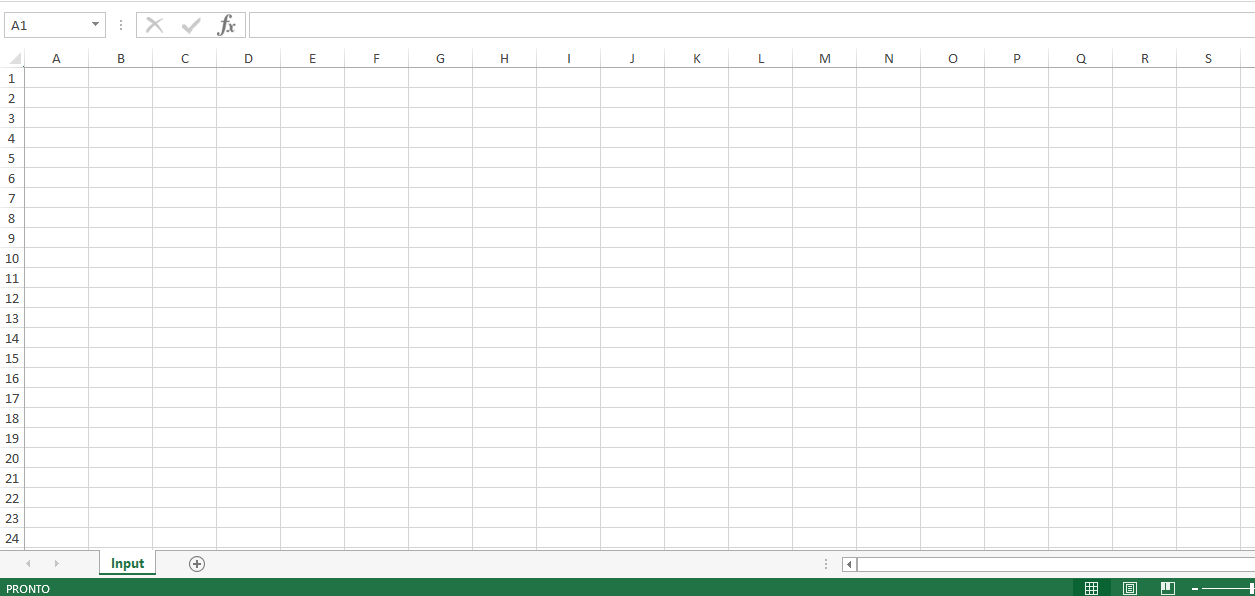
\includegraphics[width=6.28in]{images/excel-emptySheet}

\subsubsection{Populate a sheet}\label{populate-a-sheet}

To add something to an empty sheet use \texttt{writeWorkbook} function:

\begin{Shaded}
\begin{Highlighting}[]
\NormalTok{df <-}\StringTok{ }\KeywordTok{data.frame}\NormalTok{(}\StringTok{'inputType'}\NormalTok{=}\KeywordTok{c}\NormalTok{(}\StringTok{'Day'}\NormalTok{,}\StringTok{'Month'}\NormalTok{),}\StringTok{'inputValue'}\NormalTok{=}\KeywordTok{c}\NormalTok{(}\DecValTok{1}\NormalTok{,}\DecValTok{3}\NormalTok{))}
\KeywordTok{writeWorksheet}\NormalTok{(}\DataTypeTok{object =} \NormalTok{exc, }\DataTypeTok{data =} \NormalTok{df, }\DataTypeTok{sheet =} \StringTok{"Input"}\NormalTok{, }\DataTypeTok{startRow =} \DecValTok{1}\NormalTok{, }\DataTypeTok{startCol =} \DecValTok{2}\NormalTok{)}
\KeywordTok{saveWorkbook}\NormalTok{(exc)}
\end{Highlighting}
\end{Shaded}

The \texttt{df} data frame with 2 rows and 2 column is created and
\texttt{writeWorkbook()} function write the content of this data frame
in the sheet \emph{Input} starting from the cell (1,2).

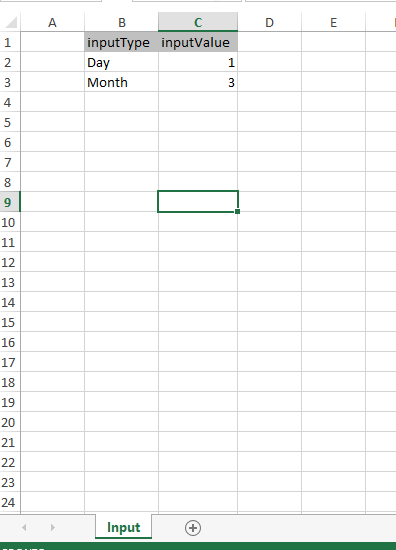
\includegraphics[width=2.64in]{images/excel-inputSheet}

\subsubsection{Create multiple sheets}\label{create-multiple-sheets}

To add other sheets to an R object workbook, use \texttt{createSheet()}
function:

\begin{Shaded}
\begin{Highlighting}[]
\CommentTok{# Add a sheet named Airquality to exc object}
\KeywordTok{createSheet}\NormalTok{(exc,}\StringTok{'Airquality'}\NormalTok{)}
\KeywordTok{saveWorkbook}\NormalTok{(exc)}
\end{Highlighting}
\end{Shaded}

Suppose we want to add a dataset to the sheet just created.\\
We want to add \texttt{airquality} dataset available in
\texttt{datasets} package, which reports daily air quality measurements
in New York, from May to September 1973.

\begin{Shaded}
\begin{Highlighting}[]
\CommentTok{# Add an empty column to airquality dataset before add it to 'Airquality' sheet}
\NormalTok{airquality$isCurrent<-}\OtherTok{NA}
\CommentTok{# Add airquality dataset to the sheet Airquality}
\KeywordTok{createName}\NormalTok{(exc, }\DataTypeTok{name=}\StringTok{'Airquality'}\NormalTok{,}\DataTypeTok{formula=}\StringTok{'Airquality!$A$1'}\NormalTok{)}
\KeywordTok{writeNamedRegion}\NormalTok{(exc, airquality, }\DataTypeTok{name =} \StringTok{'Airquality'}\NormalTok{, }\DataTypeTok{header =} \OtherTok{TRUE}\NormalTok{)}
\KeywordTok{saveWorkbook}\NormalTok{(exc)}
\end{Highlighting}
\end{Shaded}

In particular, \texttt{createName()} function creates a named region
`Airquality' starting from the cell \$A\$1 of sheet \emph{Airquality}.
In Excel, a named region/range represents cells, a range of cells, a
constant value, or a formula with a defined name which make easier to
work. It is useful for navigation, to quickly select the named range,
for reusing it when referencing it in such things as charts and
formulas, \ldots{}\\
\texttt{writeNamedRegion()} function writes \texttt{airquality} data
frame with headers \texttt{(header=TRUE)} in the named region
\emph{Airquality}.

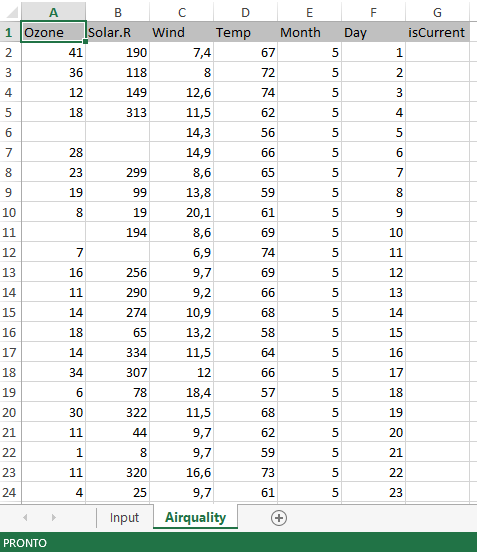
\includegraphics[width=3.18in]{images/excel-airqualitySheet}

\subsubsection{Add a formula}\label{add-a-formula}

Use \texttt{setCellFormula()} function to set cell formulas for specific
cells in a workbook.\\
The empty column \emph{isCurrent} in \emph{Airquality} sheet could be
populate with a formula that lies \emph{Input} sheet with
\emph{Airquality} sheet.

\begin{Shaded}
\begin{Highlighting}[]
\CommentTok{# Define the column index of the cell to edit}
\NormalTok{col_index <-}\StringTok{ }\KeywordTok{which}\NormalTok{(}\KeywordTok{names}\NormalTok{(airquality) ==}\StringTok{ 'isCurrent'}\NormalTok{)}
\CommentTok{# Define the excel letter for the column 'Day' and 'Month' needed by the formula }
\NormalTok{letter_day <-}\StringTok{ }\KeywordTok{idx2col}\NormalTok{(}\KeywordTok{which}\NormalTok{(}\KeywordTok{names}\NormalTok{(airquality) ==}\StringTok{ 'Day'}\NormalTok{))}
\NormalTok{letter_month <-}\StringTok{ }\KeywordTok{idx2col}\NormalTok{(}\KeywordTok{which}\NormalTok{(}\KeywordTok{names}\NormalTok{(airquality) ==}\StringTok{ 'Month'}\NormalTok{))}
\end{Highlighting}
\end{Shaded}

The function \texttt{idx2col()} returns the correspondig excel letter
for the index column. With the syntax:

\begin{Shaded}
\begin{Highlighting}[]
\NormalTok{letter_day <-}\StringTok{ }\KeywordTok{idx2col}\NormalTok{(}\KeywordTok{which}\NormalTok{(}\KeywordTok{names}\NormalTok{(airquality) ==}\StringTok{ 'Day'}\NormalTok{))}
\end{Highlighting}
\end{Shaded}

the variable \texttt{letter\_day} contains the excel letter for the
column \emph{Day}

\begin{verbatim}
## letter_day= F
\end{verbatim}

\begin{Shaded}
\begin{Highlighting}[]
\CommentTok{# Define the formula to apply to the cell}
\NormalTok{formula_xls <-}\StringTok{ }\KeywordTok{paste}\NormalTok{(}\StringTok{'IF(AND('}\NormalTok{,}
                    \NormalTok{letter_month,}
                    \DecValTok{2}\NormalTok{:(}\KeywordTok{nrow}\NormalTok{(airquality)+}\DecValTok{1}\NormalTok{),}
                    \StringTok{'=Input!C3,'}\NormalTok{,}
                    \NormalTok{letter_day,}
                    \DecValTok{2}\NormalTok{:(}\KeywordTok{nrow}\NormalTok{(airquality)+}\DecValTok{1}\NormalTok{),}
                    \StringTok{'=Input!C2)'}\NormalTok{,}
                    \StringTok{',1,0)'}\NormalTok{,}\DataTypeTok{sep=}\StringTok{''}\NormalTok{)}
\KeywordTok{setCellFormula}\NormalTok{(exc, }\DataTypeTok{sheet=}\StringTok{'Airquality'}\NormalTok{, }\DataTypeTok{row =} \DecValTok{2}\NormalTok{:(}\KeywordTok{nrow}\NormalTok{(airquality)+}\DecValTok{1}\NormalTok{), }\DataTypeTok{col =} \NormalTok{col_index, }\DataTypeTok{formula =} \NormalTok{formula_xls)}
\KeywordTok{saveWorkbook}\NormalTok{(exc)}
\end{Highlighting}
\end{Shaded}

The function \texttt{setCellFormula()} apply the formula specified by
the argument \texttt{formula} to the rows specified by the \texttt{row}
argument of the column specified by the \texttt{col} argument of the
sheet of the R object specified by the \texttt{sheet} argument.

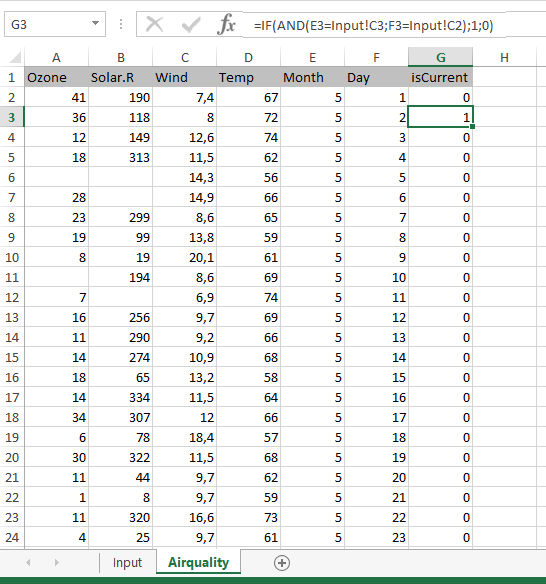
\includegraphics[width=3.64in]{images/excel-addFormula}

\subsubsection{Read an existing xlsx
file}\label{read-an-existing-xlsx-file}

To read an existing excel file, the syntax is:

\begin{Shaded}
\begin{Highlighting}[]
\CommentTok{# Excel file (with path) to be loaded into R}
\NormalTok{file_xls <-}\StringTok{ "./xlsx/newFile.xlsx"}
\end{Highlighting}
\end{Shaded}

\begin{Shaded}
\begin{Highlighting}[]
\NormalTok{exc2 <-}\StringTok{ }\KeywordTok{loadWorkbook}\NormalTok{(file_xls)}
\NormalTok{dt_air <-}\StringTok{ }\KeywordTok{readWorksheet}\NormalTok{(exc2, }\DataTypeTok{sheet =} \StringTok{'Airquality'}\NormalTok{)}
\KeywordTok{head}\NormalTok{(dt_air)}
\end{Highlighting}
\end{Shaded}

\begin{verbatim}
##   Ozone Solar.R Wind Temp Month Day isCurrent
## 1    41     190  7.4   67     5   1         0
## 2    36     118  8.0   72     5   2         0
## 3    12     149 12.6   74     5   3         0
## 4    18     313 11.5   62     5   4         0
## 5    NA      NA 14.3   56     5   5         0
## 6    28      NA 14.9   66     5   6         0
\end{verbatim}

\texttt{loadWorkbook()} function loads a Microsoft Excel workbook, in
this case ``newFile.xlsx'', into R creating a R workbook object,
\texttt{exc2}.\\
\texttt{readWorksheet()} function reads data from \emph{Airquality}
sheet of \texttt{exc2} object (the workbook that has been previously
loaded).

\subsubsection{Modify an existing xlsx
file}\label{modify-an-existing-xlsx-file}

Suppose we want to create another sheet named \emph{OzonePlot}, with a
named region \emph{OzonePlot}:

\begin{Shaded}
\begin{Highlighting}[]
\KeywordTok{createSheet}\NormalTok{(exc2, }\DataTypeTok{name =} \StringTok{"OzonePlot"}\NormalTok{)}
\KeywordTok{createName}\NormalTok{(exc2, }\DataTypeTok{name=}\StringTok{'OzonePlot'}\NormalTok{,}\DataTypeTok{formula=}\StringTok{'OzonePlot!$A$1'}\NormalTok{)}
\KeywordTok{saveWorkbook}\NormalTok{(exc2)}
\end{Highlighting}
\end{Shaded}

\texttt{createSheet()} function adds the new sheet \emph{OzonePlot} to
\texttt{exc2} object and \texttt{createName()} function creates a new
named region \emph{OzonePlot} starting from \emph{OzonePlot!\$A\$1}
cell. \texttt{saveWorkbook()} function fisically save the change done to
R object also in the corresponding xlsx file, in this case
``newFile.xlsx''.

\subsubsection{Adding a plot (image)}\label{adding-a-plot-image}

After creating a new sheet it is possible to put in this sheet a picture
of a graph created in R with the function \texttt{addImage()}:

\begin{Shaded}
\begin{Highlighting}[]
\KeywordTok{require}\NormalTok{(ggplot2)}
\CommentTok{# Generate a graph and save it in png format}
\NormalTok{fileGraph <-}\StringTok{ }\KeywordTok{paste}\NormalTok{(outDir,}\StringTok{'graph.png'}\NormalTok{,}\DataTypeTok{sep=}\StringTok{'/'}\NormalTok{)}
\KeywordTok{png}\NormalTok{(}\DataTypeTok{filename =} \NormalTok{fileGraph, }\DataTypeTok{width =} \DecValTok{800}\NormalTok{, }\DataTypeTok{height =} \DecValTok{600}\NormalTok{)}
\NormalTok{ozone_plot <-}\StringTok{ }\KeywordTok{ggplot}\NormalTok{(dt_air, }\KeywordTok{aes}\NormalTok{(}\DataTypeTok{x=}\NormalTok{Day, }\DataTypeTok{y=}\NormalTok{Ozone)) +}\StringTok{ }
\KeywordTok{geom_point}\NormalTok{() +}\StringTok{ }
\KeywordTok{geom_smooth}\NormalTok{()+}
\KeywordTok{facet_wrap}\NormalTok{(~Month, }\DataTypeTok{nrow=}\DecValTok{1}\NormalTok{)}
\KeywordTok{print}\NormalTok{(ozone_plot)}
\KeywordTok{invisible}\NormalTok{(}\KeywordTok{dev.off}\NormalTok{())}
\CommentTok{# Add image file created to 'OzonePlot' named region with its original size }
\KeywordTok{addImage}\NormalTok{(exc2, }\DataTypeTok{filename =}  \NormalTok{fileGraph, }\DataTypeTok{name =} \StringTok{'OzonePlot'}\NormalTok{, }\DataTypeTok{originalSize =} \OtherTok{TRUE}\NormalTok{)}
\KeywordTok{saveWorkbook}\NormalTok{(exc2)}
\CommentTok{# Remove the graph file created }
\KeywordTok{file.remove}\NormalTok{(fileGraph)}
\end{Highlighting}
\end{Shaded}

\begin{verbatim}
FALSE [1] TRUE
\end{verbatim}

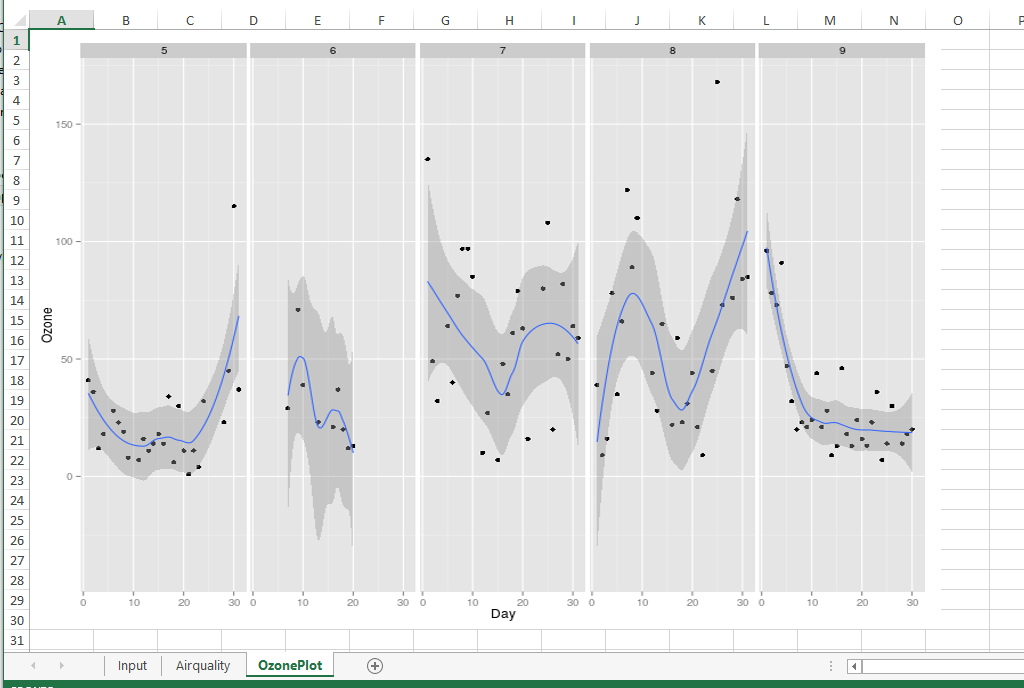
\includegraphics[width=5.12in]{images/excel-ozonePlot}

\subsection{readxl}\label{readxl}

Another R package for importing excel files into R is \texttt{readxl}.
Let us see how \texttt{readxl} works.

\begin{Shaded}
\begin{Highlighting}[]
\KeywordTok{require}\NormalTok{(readxl)}
\end{Highlighting}
\end{Shaded}

\subsubsection{Read an existing xlsx
file}\label{read-an-existing-xlsx-file-1}

To read an existing excel file, the syntax is:

\begin{Shaded}
\begin{Highlighting}[]
\CommentTok{# Excel file (with path) to be loaded into R}
\NormalTok{file_xls <-}\StringTok{ "./xlsx/newFile.xlsx"}
\end{Highlighting}
\end{Shaded}

\begin{Shaded}
\begin{Highlighting}[]
\NormalTok{ds <-}\KeywordTok{read_excel}\NormalTok{(}\DataTypeTok{path =} \NormalTok{file_xls, }\DataTypeTok{sheet =} \StringTok{'Airquality'}\NormalTok{, }\DataTypeTok{col_names =} \OtherTok{TRUE}\NormalTok{)}
\KeywordTok{head}\NormalTok{(ds)}
\end{Highlighting}
\end{Shaded}

\begin{verbatim}
## # A tibble: 6 × 7
##   Ozone Solar.R  Wind  Temp Month   Day isCurrent
##   <dbl>   <dbl> <dbl> <dbl> <dbl> <dbl>     <dbl>
## 1    41     190   7.4    67     5     1         0
## 2    36     118   8.0    72     5     2         0
## 3    12     149  12.6    74     5     3         0
## 4    18     313  11.5    62     5     4         0
## 5    NA      NA  14.3    56     5     5         0
## 6    28      NA  14.9    66     5     6         0
\end{verbatim}

\texttt{read\_excel()} function allows us to read xls and xlsx files,
specified in \texttt{path} argument. \texttt{sheet} argument specifies
the sheet to read and \texttt{col\_names} indicates if the first row has
to be used as column names (set as \texttt{TRUE}).

\clearpage

\section{Working with databases}\label{working-with-databases}


\includegraphics[width=5.81in]{images/import-db-2}

\subsection{ODBC}\label{odbc}

Open Database Connectivity (ODBC) is a standard programming language
interface for accessing database management systems (DBMS). ODBC is
independent from database systems and operating systems. An application
can use ODBC to query data from a DBMS, regardless of the operating
system or DBMS it uses. ODBC accomplishes DBMS independence by using an
ODBC driver as a translation layer between the application and the DBMS.

With the \texttt{RODBC} package R enables the use of ODBC for
interacting with databases. This solution is particularly useful when
data occupies much space, is frequently updated or shared by two or more
users. In this case, data is kept in the database. With R it is possible
to make a query in the database, load data in the R workspace and carry
out analyses.

The following code shows some examples of how to use ODBC in a MySQL
database. For the following examples to work, it is necessary to modify
the following functions with the parameters related to the available
MySQL database.

The \texttt{odbcConnect()} function establishes the connection to the
MySQL database. Its main arguments are: \texttt{dsn}, a string
containing the name of the data source, \texttt{uid} and \texttt{pwd},
i.e.~the user name and the password for the login.\\
The \texttt{sqlQuery()} function performs queries to the MySQL database.
The use of single and double quotation marks require attention. In the
following example the query is contained in a string and is delimited by
double quotation marks. The strings belonging to the query are delimited
by single quotation marks.

Finally, the \texttt{odbcClose()} function closes the connection to the
database.

\begin{Shaded}
\begin{Highlighting}[]
\CommentTok{# RODBC driver ought be configured to work properly}
\KeywordTok{require}\NormalTok{(RODBC)}
\NormalTok{conn =}\StringTok{ }\KeywordTok{odbcConnect}\NormalTok{(}\DataTypeTok{dsn =} \StringTok{"test"}\NormalTok{, }\DataTypeTok{uid =} \StringTok{"user"}\NormalTok{, }\DataTypeTok{pwd =} \StringTok{"pass"}\NormalTok{)}
\KeywordTok{sqlQuery}\NormalTok{(conn, }\StringTok{"select * from tbl where gender = 'F'"}\NormalTok{) }
\KeywordTok{odbcClose}\NormalTok{(conn)}
\end{Highlighting}
\end{Shaded}

\subsection{SQLlite}\label{sqllite}

\texttt{RSQLite} package embeds the SQLite database engine in R,
providing a DBI-compliant interface. SQLite is a public-domain,
single-user, very light-weight database engine that implements a decent
subset of the SQL 92 standard, including the core table creation,
updating, insertion, and selection operations, plus transaction
management.

\begin{Shaded}
\begin{Highlighting}[]
\KeywordTok{require}\NormalTok{(RSQLite)}
\end{Highlighting}
\end{Shaded}

The function \texttt{dbConnect} connect to a SQLite database, or creates
it if it doesn't exist, as in this case:

\begin{Shaded}
\begin{Highlighting}[]
\NormalTok{con <-}\StringTok{ }\KeywordTok{dbConnect}\NormalTok{(RSQLite::}\KeywordTok{SQLite}\NormalTok{(), }\StringTok{"mtcars.sqlite"}\NormalTok{)}
\end{Highlighting}
\end{Shaded}

To write a local data frame to the database, \texttt{dbWriteTable} is
required:

\begin{Shaded}
\begin{Highlighting}[]
\KeywordTok{dbWriteTable}\NormalTok{(con, }\StringTok{"mtcars"}\NormalTok{, mtcars)}
\end{Highlighting}
\end{Shaded}

\begin{verbatim}
## [1] TRUE
\end{verbatim}

\texttt{dbDisconnect} disconnects from the database:

\begin{Shaded}
\begin{Highlighting}[]
\KeywordTok{dbDisconnect}\NormalTok{(con)}
\end{Highlighting}
\end{Shaded}

\begin{verbatim}
## [1] TRUE
\end{verbatim}

Now \texttt{mtcars.sqlite} exists and \texttt{dbConnect} connects us to
it:

\begin{Shaded}
\begin{Highlighting}[]
\NormalTok{con <-}\StringTok{ }\KeywordTok{dbConnect}\NormalTok{(RSQLite::}\KeywordTok{SQLite}\NormalTok{(), }\StringTok{"mtcars.sqlite"}\NormalTok{)}
\end{Highlighting}
\end{Shaded}

To see a list of available SQLite tables:

\begin{Shaded}
\begin{Highlighting}[]
\KeywordTok{dbListTables}\NormalTok{(con)}
\end{Highlighting}
\end{Shaded}

\begin{verbatim}
## [1] "mtcars"
\end{verbatim}

or a list of fields in specified table:

\begin{Shaded}
\begin{Highlighting}[]
\KeywordTok{dbListFields}\NormalTok{(con, }\StringTok{"mtcars"}\NormalTok{)}
\end{Highlighting}
\end{Shaded}

\begin{verbatim}
##  [1] "row_names" "mpg"       "cyl"       "disp"      "hp"        "drat"      "wt"        "qsec"     
##  [9] "vs"        "am"        "gear"      "carb"
\end{verbatim}

The next function mimic their R/S-Plus counterpart get, assign, exists,
remove, and objects, except that they generate code that gets remotely
executed in a database engine:

\begin{Shaded}
\begin{Highlighting}[]
\KeywordTok{dbReadTable}\NormalTok{(con, }\StringTok{"mtcars"}\NormalTok{)}
\end{Highlighting}
\end{Shaded}

\begin{verbatim}
##                      mpg cyl  disp  hp drat    wt  qsec vs am gear carb
## Mazda RX4           21.0   6 160.0 110 3.90 2.620 16.46  0  1    4    4
## Mazda RX4 Wag       21.0   6 160.0 110 3.90 2.875 17.02  0  1    4    4
## Datsun 710          22.8   4 108.0  93 3.85 2.320 18.61  1  1    4    1
## Hornet 4 Drive      21.4   6 258.0 110 3.08 3.215 19.44  1  0    3    1
## Hornet Sportabout   18.7   8 360.0 175 3.15 3.440 17.02  0  0    3    2
## Valiant             18.1   6 225.0 105 2.76 3.460 20.22  1  0    3    1
## Duster 360          14.3   8 360.0 245 3.21 3.570 15.84  0  0    3    4
## Merc 240D           24.4   4 146.7  62 3.69 3.190 20.00  1  0    4    2
## Merc 230            22.8   4 140.8  95 3.92 3.150 22.90  1  0    4    2
## Merc 280            19.2   6 167.6 123 3.92 3.440 18.30  1  0    4    4
## Merc 280C           17.8   6 167.6 123 3.92 3.440 18.90  1  0    4    4
## Merc 450SE          16.4   8 275.8 180 3.07 4.070 17.40  0  0    3    3
## Merc 450SL          17.3   8 275.8 180 3.07 3.730 17.60  0  0    3    3
## Merc 450SLC         15.2   8 275.8 180 3.07 3.780 18.00  0  0    3    3
## Cadillac Fleetwood  10.4   8 472.0 205 2.93 5.250 17.98  0  0    3    4
## Lincoln Continental 10.4   8 460.0 215 3.00 5.424 17.82  0  0    3    4
## Chrysler Imperial   14.7   8 440.0 230 3.23 5.345 17.42  0  0    3    4
## Fiat 128            32.4   4  78.7  66 4.08 2.200 19.47  1  1    4    1
## Honda Civic         30.4   4  75.7  52 4.93 1.615 18.52  1  1    4    2
## Toyota Corolla      33.9   4  71.1  65 4.22 1.835 19.90  1  1    4    1
## Toyota Corona       21.5   4 120.1  97 3.70 2.465 20.01  1  0    3    1
## Dodge Challenger    15.5   8 318.0 150 2.76 3.520 16.87  0  0    3    2
## AMC Javelin         15.2   8 304.0 150 3.15 3.435 17.30  0  0    3    2
## Camaro Z28          13.3   8 350.0 245 3.73 3.840 15.41  0  0    3    4
## Pontiac Firebird    19.2   8 400.0 175 3.08 3.845 17.05  0  0    3    2
## Fiat X1-9           27.3   4  79.0  66 4.08 1.935 18.90  1  1    4    1
## Porsche 914-2       26.0   4 120.3  91 4.43 2.140 16.70  0  1    5    2
## Lotus Europa        30.4   4  95.1 113 3.77 1.513 16.90  1  1    5    2
## Ford Pantera L      15.8   8 351.0 264 4.22 3.170 14.50  0  1    5    4
## Ferrari Dino        19.7   6 145.0 175 3.62 2.770 15.50  0  1    5    6
## Maserati Bora       15.0   8 301.0 335 3.54 3.570 14.60  0  1    5    8
## Volvo 142E          21.4   4 121.0 109 4.11 2.780 18.60  1  1    4    2
\end{verbatim}

The function \texttt{dbGetQuery} send query, retrieve results and then
clear result set:

\begin{Shaded}
\begin{Highlighting}[]
\KeywordTok{dbGetQuery}\NormalTok{(con, }\StringTok{"SELECT * FROM mtcars WHERE cyl = 4"}\NormalTok{)}
\end{Highlighting}
\end{Shaded}

\begin{verbatim}
##         row_names  mpg cyl  disp  hp drat    wt  qsec vs am gear carb
## 1      Datsun 710 22.8   4 108.0  93 3.85 2.320 18.61  1  1    4    1
## 2       Merc 240D 24.4   4 146.7  62 3.69 3.190 20.00  1  0    4    2
## 3        Merc 230 22.8   4 140.8  95 3.92 3.150 22.90  1  0    4    2
## 4        Fiat 128 32.4   4  78.7  66 4.08 2.200 19.47  1  1    4    1
## 5     Honda Civic 30.4   4  75.7  52 4.93 1.615 18.52  1  1    4    2
## 6  Toyota Corolla 33.9   4  71.1  65 4.22 1.835 19.90  1  1    4    1
## 7   Toyota Corona 21.5   4 120.1  97 3.70 2.465 20.01  1  0    3    1
## 8       Fiat X1-9 27.3   4  79.0  66 4.08 1.935 18.90  1  1    4    1
## 9   Porsche 914-2 26.0   4 120.3  91 4.43 2.140 16.70  0  1    5    2
## 10   Lotus Europa 30.4   4  95.1 113 3.77 1.513 16.90  1  1    5    2
## 11     Volvo 142E 21.4   4 121.0 109 4.11 2.780 18.60  1  1    4    2
\end{verbatim}

And finally disconnect from the database:

\begin{Shaded}
\begin{Highlighting}[]
\KeywordTok{dbDisconnect}\NormalTok{(con)}
\end{Highlighting}
\end{Shaded}

\begin{verbatim}
## [1] TRUE
\end{verbatim}

\clearpage

\section{R Data Files}\label{r-data-files}

\subsection{Save R Data Files}\label{save-r-data-files}

Statistical packages often provide the opportunity to save the working
environment with all the objects it contains in their own formats. Even
if rarely used, this function is available in R as well. The format used
by R is called \texttt{Rdata} (or \texttt{Rda}).

In this way, different objects can be saved in a single file. Moreover,
all the features of a data frame which cannot be saved in a text file,
such as the levels of a factor, can be kept in the file.

To save an object of the R workspace in a file use the \texttt{save()}
function. The first argument of the function is the object to be saved,
whereas the file name is defined in the \texttt{file} argument. If the
position is not specified, R saves the file in the current directory.

\begin{Shaded}
\begin{Highlighting}[]
\CommentTok{# It creates a mtcars.Rda file in the current directory}
\KeywordTok{save}\NormalTok{(mtcars, }\DataTypeTok{file =} \StringTok{"mtcars.Rda"}\NormalTok{)}
\end{Highlighting}
\end{Shaded}

To save more than one object list their names.

\begin{Shaded}
\begin{Highlighting}[]
\CommentTok{# It creates a datasets.Rda file in the current directory}
\KeywordTok{save}\NormalTok{(mtcars, iris, }\DataTypeTok{file =} \StringTok{"datasets.Rda"}\NormalTok{)}
\end{Highlighting}
\end{Shaded}

An alternative method to save more than one object is provided by the
\texttt{list} argument. The names of the objects to be saved in a vector
can be inserted with the \texttt{list} argument. This method is
advisable when the list of the files to be saved is contained in a
vector.

\begin{Shaded}
\begin{Highlighting}[]
\CommentTok{# It creates a datasets.Rda file in the current directory}
\NormalTok{datalist =}\StringTok{ }\KeywordTok{c}\NormalTok{(}\StringTok{"mtcars"}\NormalTok{, }\StringTok{"iris"}\NormalTok{)}
\KeywordTok{save}\NormalTok{(}\DataTypeTok{list =} \NormalTok{datalist, }\DataTypeTok{file =} \StringTok{"datasets.Rda"}\NormalTok{)}
\end{Highlighting}
\end{Shaded}

\subsection{Load R Data Files}\label{load-r-data-files}

To upload \texttt{Rda} files in R use the \texttt{load()} function.

\begin{Shaded}
\begin{Highlighting}[]
\CommentTok{# It reads the datasets.Rda file previously created in the current directory}
\KeywordTok{load}\NormalTok{(}\StringTok{"datasets.Rda"}\NormalTok{)}
\end{Highlighting}
\end{Shaded}

\chapter{Introduction to dplyr}\label{introduction-to-dplyr}

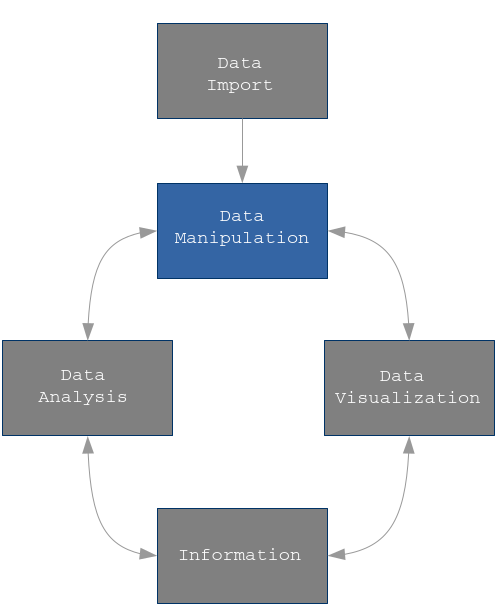
\includegraphics[width=2.94in]{images/flow-dtman}

This chapter provides an overview of data management with \texttt{R}
through the \texttt{dplyr} package.

The \texttt{dplyr} package for \texttt{R} is very powerful for data
management since:

\begin{itemize}
\tightlist
\item
  it simplifies how you can think about common data manipulation tasks;
\item
  it provides simple ``verbs'', functions that correspond to the most
  common data manipulation tasks;
\item
  it uses efficient data storage backends, so you spend less time
  waiting for the computer.
\end{itemize}

\begin{Shaded}
\begin{Highlighting}[]
\KeywordTok{require}\NormalTok{(dplyr)}
\end{Highlighting}
\end{Shaded}

In the following chapters, we will explore the innovations introduced by
\texttt{dplyr} to make our lifes easier when dealing with dataframes
manipulation tasks.\\
In particular:

\begin{itemize}
\tightlist
\item
  pipe operator (\texttt{\%\textgreater{}\%})
\item
  \texttt{tbl\_df} data frame class
\item
  \texttt{dplyr} verbs for data manipulation
\item
  \texttt{dplyr} verbs for combining data
\item
  \texttt{dplyr} with backend databases
\end{itemize}

In the following two paragraphs we will explore two important
\texttt{dplyr} innovations: pipe operator (\texttt{\%\textgreater{}\%})
and \texttt{tbl\_df} data frame class

\section{Pipe operator}\label{pipe-operator}

\texttt{dplyr} pipe operator (\texttt{\%\textgreater{}\%}) allows us to
pipe the output from one function to the input of another function. The
idea of piping is to read the functions from left to right. It is
particularly useful with nested functions (reading from the inside to
the outside) or with multiple operations.

\begin{figure}[htbp]
\centering
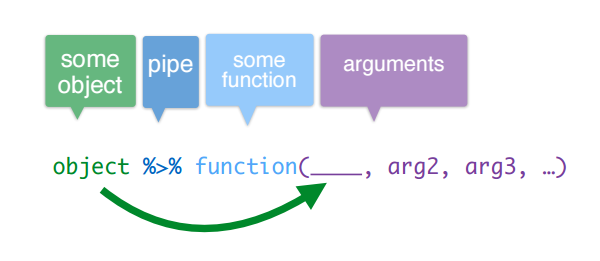
\includegraphics{./images/pipe.png}
\caption{Source: www.datacamp.com}
\end{figure}

Pipes can work with nearly any functions (\texttt{dplyr} and
not-\texttt{dplyr} functions), let us see an example.

Let us consider \texttt{bank} data set, included in \texttt{qdata}
package, which contains information about a direct marketing campaigns
of a Portuguese banking institution based on phone calls.

\begin{Shaded}
\begin{Highlighting}[]
\KeywordTok{require}\NormalTok{(qdata)}
\end{Highlighting}
\end{Shaded}

\begin{verbatim}
## Loading required package: qdata
\end{verbatim}

\begin{Shaded}
\begin{Highlighting}[]
\KeywordTok{data}\NormalTok{(bank) }
\end{Highlighting}
\end{Shaded}

Suppose we want to visualize the first rows of \texttt{bank} dataframe,
by using \texttt{head()} function.

Usually we write:

\begin{Shaded}
\begin{Highlighting}[]
\KeywordTok{head}\NormalTok{(bank)}
\end{Highlighting}
\end{Shaded}

\begin{verbatim}
## # A tibble: 6 × 20
##      id   age          job marital education default balance housing   loan contact   day  month  year
##   <int> <int>       <fctr>  <fctr>    <fctr>  <fctr>   <int>  <fctr> <fctr>  <fctr> <int> <fctr> <int>
## 1     1    58   management married  tertiary      no    2143     yes     no unknown     5    may  2008
## 2     2    44   technician  single secondary      no      29     yes     no unknown     5    may  2008
## 3     3    33 entrepreneur married secondary      no       2     yes    yes unknown     5    may  2008
## 4     4    47  blue-collar married   unknown      no    1506     yes     no unknown     5    may  2008
## 5     5    33      unknown  single   unknown      no       1      no     no unknown     5    may  2008
## 6     6    35   management married  tertiary      no     231     yes     no unknown     5    may  2008
## # ... with 7 more variables: date <dttm>, duration <int>, campaign <int>, pdays <int>, previous <int>,
## #   poutcome <fctr>, y <fctr>
\end{verbatim}

By using \texttt{\%\textgreater{}\%}, the code becomes:

\begin{Shaded}
\begin{Highlighting}[]
\NormalTok{bank %>%}\StringTok{ }\KeywordTok{head}\NormalTok{()}
\end{Highlighting}
\end{Shaded}

\begin{verbatim}
## # A tibble: 6 × 20
##      id   age          job marital education default balance housing   loan contact   day  month  year
##   <int> <int>       <fctr>  <fctr>    <fctr>  <fctr>   <int>  <fctr> <fctr>  <fctr> <int> <fctr> <int>
## 1     1    58   management married  tertiary      no    2143     yes     no unknown     5    may  2008
## 2     2    44   technician  single secondary      no      29     yes     no unknown     5    may  2008
## 3     3    33 entrepreneur married secondary      no       2     yes    yes unknown     5    may  2008
## 4     4    47  blue-collar married   unknown      no    1506     yes     no unknown     5    may  2008
## 5     5    33      unknown  single   unknown      no       1      no     no unknown     5    may  2008
## 6     6    35   management married  tertiary      no     231     yes     no unknown     5    may  2008
## # ... with 7 more variables: date <dttm>, duration <int>, campaign <int>, pdays <int>, previous <int>,
## #   poutcome <fctr>, y <fctr>
\end{verbatim}

Pipe takes the argument on the left (\texttt{bank}) and passes it to the
function on the right (\texttt{head()}). So you don't need to write the
first argument of the function.

Other arguments of the function must be added to the function itself, as
usually done. By default \texttt{head()} prints the first 6 rows of the
dataframe. Suppose we want to print 10 rows, by setting \texttt{n}
argument to 10:

\begin{Shaded}
\begin{Highlighting}[]
\NormalTok{bank %>%}\StringTok{ }\KeywordTok{head}\NormalTok{(}\DataTypeTok{n=}\DecValTok{10}\NormalTok{)}
\end{Highlighting}
\end{Shaded}

\begin{verbatim}
## # A tibble: 10 × 20
##       id   age          job  marital education default balance housing   loan contact   day  month  year
##    <int> <int>       <fctr>   <fctr>    <fctr>  <fctr>   <int>  <fctr> <fctr>  <fctr> <int> <fctr> <int>
## 1      1    58   management  married  tertiary      no    2143     yes     no unknown     5    may  2008
## 2      2    44   technician   single secondary      no      29     yes     no unknown     5    may  2008
## 3      3    33 entrepreneur  married secondary      no       2     yes    yes unknown     5    may  2008
## 4      4    47  blue-collar  married   unknown      no    1506     yes     no unknown     5    may  2008
## 5      5    33      unknown   single   unknown      no       1      no     no unknown     5    may  2008
## 6      6    35   management  married  tertiary      no     231     yes     no unknown     5    may  2008
## 7      7    28   management   single  tertiary      no     447     yes    yes unknown     5    may  2008
## 8      8    42 entrepreneur divorced  tertiary     yes       2     yes     no unknown     5    may  2008
## 9      9    58      retired  married   primary      no     121     yes     no unknown     5    may  2008
## 10    10    43   technician   single secondary      no     593     yes     no unknown     5    may  2008
## # ... with 7 more variables: date <dttm>, duration <int>, campaign <int>, pdays <int>, previous <int>,
## #   poutcome <fctr>, y <fctr>
\end{verbatim}

\subsection{\texorpdfstring{\texttt{tbl\_df}: the \texttt{dplyr} Data
Frame
Class}{tbl\_df: the dplyr Data Frame Class}}\label{tbl_df-the-dplyr-data-frame-class}

Sometimes data frames have large dimensions. \texttt{dplyr} package
provide \texttt{tbl\_df}, which is a wrapper around a data frame that
will not accidentally print a lot of data to the screen; indeed tbl
objects only print a few rows and all the columns that fit on one
screen, describing the rest of it as text.

When the class of data object is not tbl, \texttt{tbl\_df()} function
should be used.\\
Let us consider \texttt{mtcars}, a dataset included in \texttt{datasets}
package (automatically loaded at the start of an R session):

\begin{Shaded}
\begin{Highlighting}[]
\CommentTok{# Example of data frame}
\KeywordTok{class}\NormalTok{(mtcars)}
\end{Highlighting}
\end{Shaded}

\begin{verbatim}
## [1] "data.frame"
\end{verbatim}

\begin{Shaded}
\begin{Highlighting}[]
\CommentTok{# If we do not convert it as a tbl_df, all mtcars rows and columns will be printed when calling mtcars }
\KeywordTok{dim}\NormalTok{(mtcars)}
\end{Highlighting}
\end{Shaded}

\begin{verbatim}
## [1] 32 11
\end{verbatim}

\begin{Shaded}
\begin{Highlighting}[]
\NormalTok{mtcars}
\end{Highlighting}
\end{Shaded}

\begin{verbatim}
##                      mpg cyl  disp  hp drat    wt  qsec vs am gear carb
## Mazda RX4           21.0   6 160.0 110 3.90 2.620 16.46  0  1    4    4
## Mazda RX4 Wag       21.0   6 160.0 110 3.90 2.875 17.02  0  1    4    4
## Datsun 710          22.8   4 108.0  93 3.85 2.320 18.61  1  1    4    1
## Hornet 4 Drive      21.4   6 258.0 110 3.08 3.215 19.44  1  0    3    1
## Hornet Sportabout   18.7   8 360.0 175 3.15 3.440 17.02  0  0    3    2
## Valiant             18.1   6 225.0 105 2.76 3.460 20.22  1  0    3    1
## Duster 360          14.3   8 360.0 245 3.21 3.570 15.84  0  0    3    4
## Merc 240D           24.4   4 146.7  62 3.69 3.190 20.00  1  0    4    2
## Merc 230            22.8   4 140.8  95 3.92 3.150 22.90  1  0    4    2
## Merc 280            19.2   6 167.6 123 3.92 3.440 18.30  1  0    4    4
## Merc 280C           17.8   6 167.6 123 3.92 3.440 18.90  1  0    4    4
## Merc 450SE          16.4   8 275.8 180 3.07 4.070 17.40  0  0    3    3
## Merc 450SL          17.3   8 275.8 180 3.07 3.730 17.60  0  0    3    3
## Merc 450SLC         15.2   8 275.8 180 3.07 3.780 18.00  0  0    3    3
## Cadillac Fleetwood  10.4   8 472.0 205 2.93 5.250 17.98  0  0    3    4
## Lincoln Continental 10.4   8 460.0 215 3.00 5.424 17.82  0  0    3    4
## Chrysler Imperial   14.7   8 440.0 230 3.23 5.345 17.42  0  0    3    4
## Fiat 128            32.4   4  78.7  66 4.08 2.200 19.47  1  1    4    1
## Honda Civic         30.4   4  75.7  52 4.93 1.615 18.52  1  1    4    2
## Toyota Corolla      33.9   4  71.1  65 4.22 1.835 19.90  1  1    4    1
## Toyota Corona       21.5   4 120.1  97 3.70 2.465 20.01  1  0    3    1
## Dodge Challenger    15.5   8 318.0 150 2.76 3.520 16.87  0  0    3    2
## AMC Javelin         15.2   8 304.0 150 3.15 3.435 17.30  0  0    3    2
## Camaro Z28          13.3   8 350.0 245 3.73 3.840 15.41  0  0    3    4
## Pontiac Firebird    19.2   8 400.0 175 3.08 3.845 17.05  0  0    3    2
## Fiat X1-9           27.3   4  79.0  66 4.08 1.935 18.90  1  1    4    1
## Porsche 914-2       26.0   4 120.3  91 4.43 2.140 16.70  0  1    5    2
## Lotus Europa        30.4   4  95.1 113 3.77 1.513 16.90  1  1    5    2
## Ford Pantera L      15.8   8 351.0 264 4.22 3.170 14.50  0  1    5    4
## Ferrari Dino        19.7   6 145.0 175 3.62 2.770 15.50  0  1    5    6
## Maserati Bora       15.0   8 301.0 335 3.54 3.570 14.60  0  1    5    8
## Volvo 142E          21.4   4 121.0 109 4.11 2.780 18.60  1  1    4    2
\end{verbatim}

\begin{Shaded}
\begin{Highlighting}[]
\CommentTok{# dplyr version of the same data frame (tbl_df conversion)}
\NormalTok{mtcars_tbl <-}\StringTok{ }\KeywordTok{tbl_df}\NormalTok{(mtcars)}
\KeywordTok{class}\NormalTok{(mtcars_tbl)}
\end{Highlighting}
\end{Shaded}

\begin{verbatim}
## [1] "tbl_df"     "tbl"        "data.frame"
\end{verbatim}

\begin{Shaded}
\begin{Highlighting}[]
\NormalTok{mtcars_tbl}
\end{Highlighting}
\end{Shaded}

\begin{verbatim}
## # A tibble: 32 × 11
##      mpg   cyl  disp    hp  drat    wt  qsec    vs    am  gear  carb
## *  <dbl> <dbl> <dbl> <dbl> <dbl> <dbl> <dbl> <dbl> <dbl> <dbl> <dbl>
## 1   21.0     6 160.0   110  3.90 2.620 16.46     0     1     4     4
## 2   21.0     6 160.0   110  3.90 2.875 17.02     0     1     4     4
## 3   22.8     4 108.0    93  3.85 2.320 18.61     1     1     4     1
## 4   21.4     6 258.0   110  3.08 3.215 19.44     1     0     3     1
## 5   18.7     8 360.0   175  3.15 3.440 17.02     0     0     3     2
## 6   18.1     6 225.0   105  2.76 3.460 20.22     1     0     3     1
## 7   14.3     8 360.0   245  3.21 3.570 15.84     0     0     3     4
## 8   24.4     4 146.7    62  3.69 3.190 20.00     1     0     4     2
## 9   22.8     4 140.8    95  3.92 3.150 22.90     1     0     4     2
## 10  19.2     6 167.6   123  3.92 3.440 18.30     1     0     4     4
## # ... with 22 more rows
\end{verbatim}

\section{Verb Functions}\label{verb-functions}

\begin{Shaded}
\begin{Highlighting}[]
\KeywordTok{require}\NormalTok{(dplyr)}
\KeywordTok{require}\NormalTok{(qdata)}
\end{Highlighting}
\end{Shaded}

\texttt{dplyr} aims to provide a function for each basic verb of data
manipulating.

All these functions are very similar:

\begin{itemize}
\tightlist
\item
  the first argument is a data frame;
\item
  the subsequent arguments describe what to do with it, and you can
  refer to columns in the data frame directly without using \$. Note
  that the column names must be unquoted;
\item
  the result is a new data frame.
\end{itemize}

Together these properties make it easy to chain together multiple simple
steps to achieve a complex result.

These five functions provide the basis of a language of data
manipulation. At the most basic level, you can only alter a tidy data
frame in five useful ways:

\begin{enumerate}
\def\labelenumi{\arabic{enumi}.}
\tightlist
\item
  select variables of interest: \texttt{select()};
\item
  filter records of interest: \texttt{filter()};
\item
  reorder the rows: \texttt{arrange()};
\item
  add new variables that are functions of existing variables:
  \texttt{mutate()};
\item
  collapse many values to a summary: \texttt{summarise()}.
\end{enumerate}

In the following examples we will refer to \texttt{bank} data set which
contains information about a direct marketing campaigns of a Portuguese
banking institution based on phone calls.

\begin{Shaded}
\begin{Highlighting}[]
\KeywordTok{data}\NormalTok{(bank) }
\end{Highlighting}
\end{Shaded}

\clearpage

\subsection{\texorpdfstring{\texttt{select()}}{select()}}\label{select}

Often you work with large datasets with many columns where only a few
are actually of interest to you.

\texttt{select()} allows you to rapidly zoom in on a useful subset of
columns.

\begin{figure}[htbp]
\centering
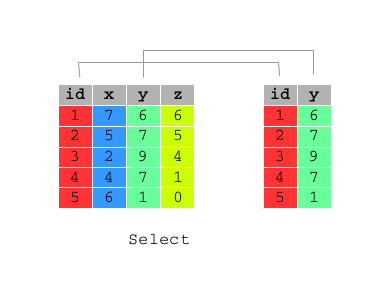
\includegraphics{images/sel.png}
\caption{}
\end{figure}

The first argument is the name of the data frame, and the second and
subsequent are the name of column/s of that data frame you want to
select:

\begin{Shaded}
\begin{Highlighting}[]
\CommentTok{# Select columns: year, month and day of bank data frame}
\KeywordTok{select}\NormalTok{(bank, year, month, day)}
\end{Highlighting}
\end{Shaded}

\begin{verbatim}
## # A tibble: 45,211 × 3
##     year  month   day
##    <int> <fctr> <int>
## 1   2008    may     5
## 2   2008    may     5
## 3   2008    may     5
## 4   2008    may     5
## 5   2008    may     5
## 6   2008    may     5
## 7   2008    may     5
## 8   2008    may     5
## 9   2008    may     5
## 10  2008    may     5
## # ... with 45,201 more rows
\end{verbatim}

\begin{Shaded}
\begin{Highlighting}[]
\CommentTok{# Select columns: year, month and day of bank data frame}
\NormalTok{bank %>%}\StringTok{ }\KeywordTok{select}\NormalTok{(year:day)}
\end{Highlighting}
\end{Shaded}

\begin{verbatim}
## # A tibble: 45,211 × 3
##     year  month   day
##    <int> <fctr> <int>
## 1   2008    may     5
## 2   2008    may     5
## 3   2008    may     5
## 4   2008    may     5
## 5   2008    may     5
## 6   2008    may     5
## 7   2008    may     5
## 8   2008    may     5
## 9   2008    may     5
## 10  2008    may     5
## # ... with 45,201 more rows
\end{verbatim}

\begin{Shaded}
\begin{Highlighting}[]
\CommentTok{# Select all columns of bank data frame apart from: year, month and day}
\NormalTok{bank %>%}\StringTok{ }\KeywordTok{select}\NormalTok{(-(year:day))}
\end{Highlighting}
\end{Shaded}

\begin{verbatim}
## # A tibble: 45,211 × 17
##       id   age          job  marital education default balance housing   loan contact       date duration
##    <int> <int>       <fctr>   <fctr>    <fctr>  <fctr>   <int>  <fctr> <fctr>  <fctr>     <dttm>    <int>
## 1      1    58   management  married  tertiary      no    2143     yes     no unknown 2008-05-05      261
## 2      2    44   technician   single secondary      no      29     yes     no unknown 2008-05-05      151
## 3      3    33 entrepreneur  married secondary      no       2     yes    yes unknown 2008-05-05       76
## 4      4    47  blue-collar  married   unknown      no    1506     yes     no unknown 2008-05-05       92
## 5      5    33      unknown   single   unknown      no       1      no     no unknown 2008-05-05      198
## 6      6    35   management  married  tertiary      no     231     yes     no unknown 2008-05-05      139
## 7      7    28   management   single  tertiary      no     447     yes    yes unknown 2008-05-05      217
## 8      8    42 entrepreneur divorced  tertiary     yes       2     yes     no unknown 2008-05-05      380
## 9      9    58      retired  married   primary      no     121     yes     no unknown 2008-05-05       50
## 10    10    43   technician   single secondary      no     593     yes     no unknown 2008-05-05       55
## # ... with 45,201 more rows, and 5 more variables: campaign <int>, pdays <int>, previous <int>,
## #   poutcome <fctr>, y <fctr>
\end{verbatim}

You can rename variables with \texttt{select()} by using named
arguments:

\begin{Shaded}
\begin{Highlighting}[]
\CommentTok{# Rename id variable as ID}
\NormalTok{bank %>%}\StringTok{ }\KeywordTok{select}\NormalTok{(}\DataTypeTok{ID =} \NormalTok{id)}
\end{Highlighting}
\end{Shaded}

\begin{verbatim}
## # A tibble: 45,211 × 1
##       ID
##    <int>
## 1      1
## 2      2
## 3      3
## 4      4
## 5      5
## 6      6
## 7      7
## 8      8
## 9      9
## 10    10
## # ... with 45,201 more rows
\end{verbatim}

\clearpage

\subsection{\texorpdfstring{\texttt{filter()}}{filter()}}\label{filter}

\texttt{filter()} allows you to select a subset of the rows of a data
frame.

\begin{figure}[htbp]
\centering
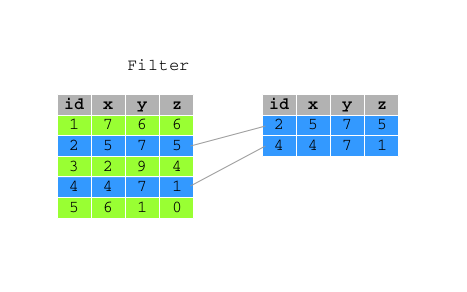
\includegraphics{images/fil.png}
\caption{}
\end{figure}

The first argument is the name of the data frame, and the second and
subsequent are filtering expressions evaluated in the context of that
data frame.

For example, you can select all calls made to students whit balance
above 20,000:

\begin{Shaded}
\begin{Highlighting}[]
\KeywordTok{filter}\NormalTok{(bank, job ==}\StringTok{ "student"}\NormalTok{, balance >}\StringTok{ }\DecValTok{20000}\NormalTok{)}
\end{Highlighting}
\end{Shaded}

\begin{verbatim}
## # A tibble: 3 × 20
##      id   age     job marital education default balance housing   loan  contact   day  month  year
##   <int> <int>  <fctr>  <fctr>    <fctr>  <fctr>   <int>  <fctr> <fctr>   <fctr> <int> <fctr> <int>
## 1 31125    24 student  single secondary      no   23878      no     no cellular    18    feb  2009
## 2 39536    24 student  single secondary      no   23878      no     no cellular    26    may  2009
## 3 41923    27 student  single  tertiary      no   24025      no     no cellular    21    oct  2009
## # ... with 7 more variables: date <dttm>, duration <int>, campaign <int>, pdays <int>, previous <int>,
## #   poutcome <fctr>, y <fctr>
\end{verbatim}

\texttt{filter()} allows you to give it any number of filtering
conditions which are joined together with \texttt{\&} and/or the other
operators.

\begin{Shaded}
\begin{Highlighting}[]
\CommentTok{# Select all calls made to student of 18 years }
\NormalTok{bank %>%}\StringTok{ }\KeywordTok{filter}\NormalTok{(age ==}\StringTok{ }\DecValTok{18} \NormalTok{&}\StringTok{ }\NormalTok{job ==}\StringTok{ "student"}\NormalTok{)}
\end{Highlighting}
\end{Shaded}

\begin{verbatim}
## # A tibble: 12 × 20
##       id   age     job marital education default balance housing   loan   contact   day  month  year
##    <int> <int>  <fctr>  <fctr>    <fctr>  <fctr>   <int>  <fctr> <fctr>    <fctr> <int> <fctr> <int>
## 1  40737    18 student  single   primary      no    1944      no     no telephone    10    aug  2009
## 2  40745    18 student  single   unknown      no     108      no     no  cellular    10    aug  2009
## 3  40888    18 student  single   primary      no     608      no     no  cellular    12    aug  2009
## 4  41223    18 student  single   unknown      no      35      no     no telephone    21    aug  2009
## 5  41253    18 student  single secondary      no       5      no     no  cellular    24    aug  2009
## 6  41274    18 student  single   unknown      no       3      no     no  cellular    25    aug  2009
## 7  41488    18 student  single   unknown      no     108      no     no  cellular     8    sep  2009
## 8  42147    18 student  single secondary      no     156      no     no  cellular     4    nov  2009
## 9  42275    18 student  single   primary      no     608      no     no  cellular    13    nov  2009
## 10 42955    18 student  single   unknown      no     108      no     no  cellular     9    feb  2010
## 11 43638    18 student  single   unknown      no     348      no     no  cellular     5    may  2010
## 12 44645    18 student  single   unknown      no     438      no     no  cellular     1    sep  2010
## # ... with 7 more variables: date <dttm>, duration <int>, campaign <int>, pdays <int>, previous <int>,
## #   poutcome <fctr>, y <fctr>
\end{verbatim}

\begin{Shaded}
\begin{Highlighting}[]
\CommentTok{# Select all calls made to people of 18 or 95 years}
\NormalTok{bank %>%}\StringTok{ }\KeywordTok{filter}\NormalTok{(age ==}\StringTok{ }\DecValTok{18} \NormalTok{|}\StringTok{ }\NormalTok{age ==}\StringTok{ }\DecValTok{95}\NormalTok{)}
\end{Highlighting}
\end{Shaded}

\begin{verbatim}
## # A tibble: 14 × 20
##       id   age     job  marital education default balance housing   loan   contact   day  month  year
##    <int> <int>  <fctr>   <fctr>    <fctr>  <fctr>   <int>  <fctr> <fctr>    <fctr> <int> <fctr> <int>
## 1  33700    95 retired divorced   primary      no    2282      no     no telephone    21    apr  2009
## 2  40737    18 student   single   primary      no    1944      no     no telephone    10    aug  2009
## 3  40745    18 student   single   unknown      no     108      no     no  cellular    10    aug  2009
## 4  40888    18 student   single   primary      no     608      no     no  cellular    12    aug  2009
## 5  41223    18 student   single   unknown      no      35      no     no telephone    21    aug  2009
## 6  41253    18 student   single secondary      no       5      no     no  cellular    24    aug  2009
## 7  41274    18 student   single   unknown      no       3      no     no  cellular    25    aug  2009
## 8  41488    18 student   single   unknown      no     108      no     no  cellular     8    sep  2009
## 9  41664    95 retired  married secondary      no       0      no     no telephone     1    oct  2009
## 10 42147    18 student   single secondary      no     156      no     no  cellular     4    nov  2009
## 11 42275    18 student   single   primary      no     608      no     no  cellular    13    nov  2009
## 12 42955    18 student   single   unknown      no     108      no     no  cellular     9    feb  2010
## 13 43638    18 student   single   unknown      no     348      no     no  cellular     5    may  2010
## 14 44645    18 student   single   unknown      no     438      no     no  cellular     1    sep  2010
## # ... with 7 more variables: date <dttm>, duration <int>, campaign <int>, pdays <int>, previous <int>,
## #   poutcome <fctr>, y <fctr>
\end{verbatim}

\texttt{filter()} can be used also with \texttt{\%in\%} to establish
conditions under which filter:

\begin{Shaded}
\begin{Highlighting}[]
\CommentTok{# Select all calls made to people of 18 or 95 years}
\NormalTok{bank %>%}\StringTok{ }\KeywordTok{filter}\NormalTok{(age %in%}\StringTok{ }\KeywordTok{c}\NormalTok{(}\DecValTok{18}\NormalTok{,}\DecValTok{95}\NormalTok{))}
\end{Highlighting}
\end{Shaded}

\begin{verbatim}
## # A tibble: 14 × 20
##       id   age     job  marital education default balance housing   loan   contact   day  month  year
##    <int> <int>  <fctr>   <fctr>    <fctr>  <fctr>   <int>  <fctr> <fctr>    <fctr> <int> <fctr> <int>
## 1  33700    95 retired divorced   primary      no    2282      no     no telephone    21    apr  2009
## 2  40737    18 student   single   primary      no    1944      no     no telephone    10    aug  2009
## 3  40745    18 student   single   unknown      no     108      no     no  cellular    10    aug  2009
## 4  40888    18 student   single   primary      no     608      no     no  cellular    12    aug  2009
## 5  41223    18 student   single   unknown      no      35      no     no telephone    21    aug  2009
## 6  41253    18 student   single secondary      no       5      no     no  cellular    24    aug  2009
## 7  41274    18 student   single   unknown      no       3      no     no  cellular    25    aug  2009
## 8  41488    18 student   single   unknown      no     108      no     no  cellular     8    sep  2009
## 9  41664    95 retired  married secondary      no       0      no     no telephone     1    oct  2009
## 10 42147    18 student   single secondary      no     156      no     no  cellular     4    nov  2009
## 11 42275    18 student   single   primary      no     608      no     no  cellular    13    nov  2009
## 12 42955    18 student   single   unknown      no     108      no     no  cellular     9    feb  2010
## 13 43638    18 student   single   unknown      no     348      no     no  cellular     5    may  2010
## 14 44645    18 student   single   unknown      no     438      no     no  cellular     1    sep  2010
## # ... with 7 more variables: date <dttm>, duration <int>, campaign <int>, pdays <int>, previous <int>,
## #   poutcome <fctr>, y <fctr>
\end{verbatim}

An other example is:

\begin{Shaded}
\begin{Highlighting}[]
\CommentTok{# Select all calls made to people whose job is admin. or technician }
\NormalTok{bank %>%}\StringTok{ }\KeywordTok{filter}\NormalTok{(job %in%}\StringTok{ }\KeywordTok{c}\NormalTok{(}\StringTok{"admin."}\NormalTok{,}\StringTok{"technician"}\NormalTok{))}
\end{Highlighting}
\end{Shaded}

\begin{verbatim}
## # A tibble: 12,768 × 20
##       id   age        job  marital education default balance housing   loan contact   day  month  year
##    <int> <int>     <fctr>   <fctr>    <fctr>  <fctr>   <int>  <fctr> <fctr>  <fctr> <int> <fctr> <int>
## 1      2    44 technician   single secondary      no      29     yes     no unknown     5    may  2008
## 2     10    43 technician   single secondary      no     593     yes     no unknown     5    may  2008
## 3     11    41     admin. divorced secondary      no     270     yes     no unknown     5    may  2008
## 4     12    29     admin.   single secondary      no     390     yes     no unknown     5    may  2008
## 5     13    53 technician  married secondary      no       6     yes     no unknown     5    may  2008
## 6     14    58 technician  married   unknown      no      71     yes     no unknown     5    may  2008
## 7     17    45     admin.   single   unknown      no      13     yes     no unknown     5    may  2008
## 8     26    44     admin.  married secondary      no    -372     yes     no unknown     5    may  2008
## 9     30    36 technician   single secondary      no     265     yes    yes unknown     5    may  2008
## 10    31    57 technician  married secondary      no     839      no    yes unknown     5    may  2008
## # ... with 12,758 more rows, and 7 more variables: date <dttm>, duration <int>, campaign <int>,
## #   pdays <int>, previous <int>, poutcome <fctr>, y <fctr>
\end{verbatim}

\begin{Shaded}
\begin{Highlighting}[]
\CommentTok{# Select all calls made to people whose job is admin. or technician }
\NormalTok{bank %>%}\StringTok{ }\KeywordTok{filter}\NormalTok{(job ==}\StringTok{ "admin."} \NormalTok{|}\StringTok{ }\NormalTok{job ==}\StringTok{ "technician"}\NormalTok{)}
\end{Highlighting}
\end{Shaded}

\begin{verbatim}
## # A tibble: 12,768 × 20
##       id   age        job  marital education default balance housing   loan contact   day  month  year
##    <int> <int>     <fctr>   <fctr>    <fctr>  <fctr>   <int>  <fctr> <fctr>  <fctr> <int> <fctr> <int>
## 1      2    44 technician   single secondary      no      29     yes     no unknown     5    may  2008
## 2     10    43 technician   single secondary      no     593     yes     no unknown     5    may  2008
## 3     11    41     admin. divorced secondary      no     270     yes     no unknown     5    may  2008
## 4     12    29     admin.   single secondary      no     390     yes     no unknown     5    may  2008
## 5     13    53 technician  married secondary      no       6     yes     no unknown     5    may  2008
## 6     14    58 technician  married   unknown      no      71     yes     no unknown     5    may  2008
## 7     17    45     admin.   single   unknown      no      13     yes     no unknown     5    may  2008
## 8     26    44     admin.  married secondary      no    -372     yes     no unknown     5    may  2008
## 9     30    36 technician   single secondary      no     265     yes    yes unknown     5    may  2008
## 10    31    57 technician  married secondary      no     839      no    yes unknown     5    may  2008
## # ... with 12,758 more rows, and 7 more variables: date <dttm>, duration <int>, campaign <int>,
## #   pdays <int>, previous <int>, poutcome <fctr>, y <fctr>
\end{verbatim}

\clearpage

\subsection{\texorpdfstring{\texttt{arrange()}}{arrange()}}\label{arrange}

Function \texttt{arrange()} reorders a data frame by one or more
variables. If you provide more than one column name, each additional
column will be used to break ties in the values of preceding columns:

\begin{figure}[htbp]
\centering
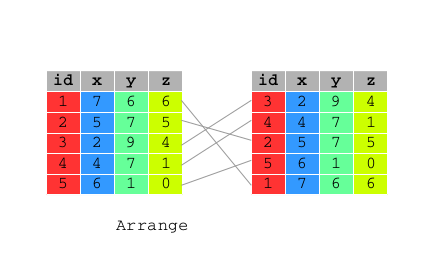
\includegraphics{images/arr.png}
\caption{}
\end{figure}

The first argument is the name of the data frame, and the second and
subsequent are the name of columns of that data frame you want to order
by.\\
You may want to order the \texttt{bank} data frame by the balance of the
account in ascending order:

\begin{Shaded}
\begin{Highlighting}[]
\KeywordTok{arrange}\NormalTok{(bank, balance)}
\end{Highlighting}
\end{Shaded}

\begin{verbatim}
## # A tibble: 45,211 × 20
##       id   age           job  marital education default balance housing   loan  contact   day  month  year
##    <int> <int>        <fctr>   <fctr>    <fctr>  <fctr>   <int>  <fctr> <fctr>   <fctr> <int> <fctr> <int>
## 1  12910    26   blue-collar   single secondary     yes   -8019      no    yes cellular     7    jul  2008
## 2  15683    49    management  married  tertiary     yes   -6847      no    yes cellular    21    jul  2008
## 3  38737    60    management divorced  tertiary      no   -4057     yes     no cellular    18    may  2009
## 4   7414    43    management  married  tertiary     yes   -3372     yes     no  unknown    29    may  2008
## 5   1897    57 self-employed  married  tertiary     yes   -3313     yes    yes  unknown     9    may  2008
## 6  32714    39 self-employed  married  tertiary      no   -3058     yes    yes cellular    17    apr  2009
## 7  18574    40    technician  married  tertiary     yes   -2827     yes    yes cellular    31    jul  2008
## 8  31510    52    management  married  tertiary      no   -2712     yes    yes cellular     2    apr  2009
## 9  25120    49   blue-collar   single   primary     yes   -2604     yes     no cellular    18    nov  2008
## 10 14435    51    management divorced  tertiary      no   -2282     yes    yes cellular    14    jul  2008
## # ... with 45,201 more rows, and 7 more variables: date <dttm>, duration <int>, campaign <int>,
## #   pdays <int>, previous <int>, poutcome <fctr>, y <fctr>
\end{verbatim}

or in descending order by using function \texttt{desc()} within
\texttt{arrange()}:

\begin{Shaded}
\begin{Highlighting}[]
\NormalTok{bank %>%}\StringTok{ }\KeywordTok{arrange}\NormalTok{(}\KeywordTok{desc}\NormalTok{(balance))}
\end{Highlighting}
\end{Shaded}

\begin{verbatim}
## # A tibble: 45,211 × 20
##       id   age          job  marital education default balance housing   loan   contact   day  month  year
##    <int> <int>       <fctr>   <fctr>    <fctr>  <fctr>   <int>  <fctr> <fctr>    <fctr> <int> <fctr> <int>
## 1  39990    51   management   single  tertiary      no  102127      no     no  cellular     3    jun  2009
## 2  26228    59   management  married  tertiary      no   98417      no     no telephone    20    nov  2008
## 3  42559    84      retired  married secondary      no   81204      no     no telephone    28    dec  2009
## 4  43394    84      retired  married secondary      no   81204      no     no telephone     1    apr  2010
## 5  41694    60      retired  married   primary      no   71188      no     no  cellular     6    oct  2009
## 6  19786    56   management divorced  tertiary      no   66721      no     no  cellular     8    aug  2008
## 7  21193    52  blue-collar  married   primary      no   66653      no     no  cellular    14    aug  2008
## 8  19421    59       admin.  married   unknown      no   64343      no     no  cellular     6    aug  2008
## 9  41375    32 entrepreneur   single  tertiary      no   59649      no     no  cellular     1    sep  2009
## 10 12927    56  blue-collar  married secondary      no   58932      no     no telephone     7    jul  2008
## # ... with 45,201 more rows, and 7 more variables: date <dttm>, duration <int>, campaign <int>,
## #   pdays <int>, previous <int>, poutcome <fctr>, y <fctr>
\end{verbatim}

You can order a data frame by one or more than one variables.

Ordering data frame bank by \texttt{age} first and descending
\texttt{balance} afterward requires:

\begin{Shaded}
\begin{Highlighting}[]
\NormalTok{bank %>%}\StringTok{ }\KeywordTok{arrange}\NormalTok{(age, }\KeywordTok{desc}\NormalTok{(balance))}
\end{Highlighting}
\end{Shaded}

\begin{verbatim}
## # A tibble: 45,211 × 20
##       id   age     job marital education default balance housing   loan   contact   day  month  year
##    <int> <int>  <fctr>  <fctr>    <fctr>  <fctr>   <int>  <fctr> <fctr>    <fctr> <int> <fctr> <int>
## 1  40737    18 student  single   primary      no    1944      no     no telephone    10    aug  2009
## 2  40888    18 student  single   primary      no     608      no     no  cellular    12    aug  2009
## 3  42275    18 student  single   primary      no     608      no     no  cellular    13    nov  2009
## 4  44645    18 student  single   unknown      no     438      no     no  cellular     1    sep  2010
## 5  43638    18 student  single   unknown      no     348      no     no  cellular     5    may  2010
## 6  42147    18 student  single secondary      no     156      no     no  cellular     4    nov  2009
## 7  40745    18 student  single   unknown      no     108      no     no  cellular    10    aug  2009
## 8  41488    18 student  single   unknown      no     108      no     no  cellular     8    sep  2009
## 9  42955    18 student  single   unknown      no     108      no     no  cellular     9    feb  2010
## 10 41223    18 student  single   unknown      no      35      no     no telephone    21    aug  2009
## # ... with 45,201 more rows, and 7 more variables: date <dttm>, duration <int>, campaign <int>,
## #   pdays <int>, previous <int>, poutcome <fctr>, y <fctr>
\end{verbatim}

\clearpage

\subsection{\texorpdfstring{\texttt{mutate()}}{mutate()}}\label{mutate}

As well as selecting from the set of existing columns, it's often useful
to add new columns that are functions of existing columns. This is the
job of \texttt{mutate()}:

\begin{figure}[htbp]
\centering
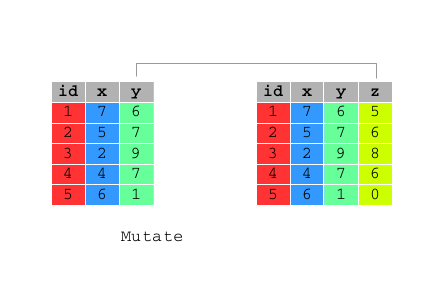
\includegraphics{images/mut.png}
\caption{}
\end{figure}

The first argument is the name of the data frame, and the second and
subsequent are expressions for creating new columns to add to that data
frame or for modifying the existing ones:

\begin{Shaded}
\begin{Highlighting}[]
\NormalTok{df <-}\StringTok{ }\KeywordTok{data.frame}\NormalTok{(}\DataTypeTok{x =} \DecValTok{1}\NormalTok{:}\DecValTok{3}\NormalTok{, }\DataTypeTok{y =} \DecValTok{3}\NormalTok{:}\DecValTok{1}\NormalTok{)}

\KeywordTok{mutate}\NormalTok{(df, }\DataTypeTok{x1 =} \NormalTok{x}\DecValTok{+1}\NormalTok{)}
\end{Highlighting}
\end{Shaded}

\begin{verbatim}
##   x y x1
## 1 1 3  2
## 2 2 2  3
## 3 3 1  4
\end{verbatim}

\begin{Shaded}
\begin{Highlighting}[]
\KeywordTok{mutate}\NormalTok{(df, }\DataTypeTok{x =} \NormalTok{x}\DecValTok{+1}\NormalTok{)}
\end{Highlighting}
\end{Shaded}

\begin{verbatim}
##   x y
## 1 2 3
## 2 3 2
## 3 4 1
\end{verbatim}

\begin{Shaded}
\begin{Highlighting}[]
\KeywordTok{mutate}\NormalTok{(df, }\DataTypeTok{x =} \NormalTok{x}\DecValTok{+1}\NormalTok{, }\DataTypeTok{y =} \NormalTok{x}\DecValTok{+1}\NormalTok{)}
\end{Highlighting}
\end{Shaded}

\begin{verbatim}
##   x y
## 1 2 3
## 2 3 4
## 3 4 5
\end{verbatim}

\begin{Shaded}
\begin{Highlighting}[]
\KeywordTok{mutate}\NormalTok{(df, }\DataTypeTok{x1 =} \NormalTok{x}\DecValTok{+1}\NormalTok{, }\DataTypeTok{y1 =} \NormalTok{x1}\DecValTok{+1}\NormalTok{)}
\end{Highlighting}
\end{Shaded}

\begin{verbatim}
##   x y x1 y1
## 1 1 3  2  3
## 2 2 2  3  4
## 3 3 1  4  5
\end{verbatim}

\begin{Shaded}
\begin{Highlighting}[]
\KeywordTok{mutate}\NormalTok{(df, }\DataTypeTok{y1 =} \NormalTok{x}\DecValTok{+1}\NormalTok{, }\DataTypeTok{x1 =} \NormalTok{x}\DecValTok{+1}\NormalTok{)}
\end{Highlighting}
\end{Shaded}

\begin{verbatim}
##   x y y1 x1
## 1 1 3  2  2
## 2 2 2  3  3
## 3 3 1  4  4
\end{verbatim}

\begin{Shaded}
\begin{Highlighting}[]
\KeywordTok{mutate}\NormalTok{(df, }\DataTypeTok{xx =} \NormalTok{x)}
\end{Highlighting}
\end{Shaded}

\begin{verbatim}
##   x y xx
## 1 1 3  1
## 2 2 2  2
## 3 3 1  3
\end{verbatim}

\begin{Shaded}
\begin{Highlighting}[]
\CommentTok{# generate a variable indicating the total number of times each person has been contacted }
\CommentTok{# during this campaign and during the previous ones }
\KeywordTok{mutate}\NormalTok{(bank, }\DataTypeTok{contacts_n =} \NormalTok{campaign +}\StringTok{ }\NormalTok{previous)}
\end{Highlighting}
\end{Shaded}

\begin{verbatim}
## # A tibble: 45,211 × 21
##       id   age          job  marital education default balance housing   loan contact   day  month  year
##    <int> <int>       <fctr>   <fctr>    <fctr>  <fctr>   <int>  <fctr> <fctr>  <fctr> <int> <fctr> <int>
## 1      1    58   management  married  tertiary      no    2143     yes     no unknown     5    may  2008
## 2      2    44   technician   single secondary      no      29     yes     no unknown     5    may  2008
## 3      3    33 entrepreneur  married secondary      no       2     yes    yes unknown     5    may  2008
## 4      4    47  blue-collar  married   unknown      no    1506     yes     no unknown     5    may  2008
## 5      5    33      unknown   single   unknown      no       1      no     no unknown     5    may  2008
## 6      6    35   management  married  tertiary      no     231     yes     no unknown     5    may  2008
## 7      7    28   management   single  tertiary      no     447     yes    yes unknown     5    may  2008
## 8      8    42 entrepreneur divorced  tertiary     yes       2     yes     no unknown     5    may  2008
## 9      9    58      retired  married   primary      no     121     yes     no unknown     5    may  2008
## 10    10    43   technician   single secondary      no     593     yes     no unknown     5    may  2008
## # ... with 45,201 more rows, and 8 more variables: date <dttm>, duration <int>, campaign <int>,
## #   pdays <int>, previous <int>, poutcome <fctr>, y <fctr>, contacts_n <int>
\end{verbatim}

\texttt{mutate()} allows you to refer to columns that you just created:

\begin{Shaded}
\begin{Highlighting}[]
\CommentTok{# generate two variable: one indicating the year of birth and one the year of birth without century }
\NormalTok{bank %>%}\StringTok{ }\KeywordTok{mutate}\NormalTok{(}\DataTypeTok{year_of_birth =} \NormalTok{year -}\StringTok{ }\NormalTok{age, }\DataTypeTok{year_of_birth_no_century =} \NormalTok{year_of_birth -}\StringTok{ }\DecValTok{1900}\NormalTok{)}
\end{Highlighting}
\end{Shaded}

\begin{verbatim}
## # A tibble: 45,211 × 22
##       id   age          job  marital education default balance housing   loan contact   day  month  year
##    <int> <int>       <fctr>   <fctr>    <fctr>  <fctr>   <int>  <fctr> <fctr>  <fctr> <int> <fctr> <int>
## 1      1    58   management  married  tertiary      no    2143     yes     no unknown     5    may  2008
## 2      2    44   technician   single secondary      no      29     yes     no unknown     5    may  2008
## 3      3    33 entrepreneur  married secondary      no       2     yes    yes unknown     5    may  2008
## 4      4    47  blue-collar  married   unknown      no    1506     yes     no unknown     5    may  2008
## 5      5    33      unknown   single   unknown      no       1      no     no unknown     5    may  2008
## 6      6    35   management  married  tertiary      no     231     yes     no unknown     5    may  2008
## 7      7    28   management   single  tertiary      no     447     yes    yes unknown     5    may  2008
## 8      8    42 entrepreneur divorced  tertiary     yes       2     yes     no unknown     5    may  2008
## 9      9    58      retired  married   primary      no     121     yes     no unknown     5    may  2008
## 10    10    43   technician   single secondary      no     593     yes     no unknown     5    may  2008
## # ... with 45,201 more rows, and 9 more variables: date <dttm>, duration <int>, campaign <int>,
## #   pdays <int>, previous <int>, poutcome <fctr>, y <fctr>, year_of_birth <int>,
## #   year_of_birth_no_century <dbl>
\end{verbatim}

\clearpage

\subsection{\texorpdfstring{\texttt{summarise()}}{summarise()}}\label{summarise}

The last verb is \texttt{summarise()}, which collapses a data frame to a
single row.

The first argument is the name of the data frame, and the second and
subsequent are summarising expressions.

\begin{Shaded}
\begin{Highlighting}[]
\CommentTok{# Compute the mean of balance variable of bank data frame}
\NormalTok{bank %>%}\StringTok{ }\KeywordTok{summarise}\NormalTok{(}\DataTypeTok{mean_balance =} \KeywordTok{mean}\NormalTok{(balance, }\DataTypeTok{na.rm =} \OtherTok{TRUE}\NormalTok{))}
\end{Highlighting}
\end{Shaded}

\begin{verbatim}
## # A tibble: 1 × 1
##   mean_balance
##          <dbl>
## 1     1362.272
\end{verbatim}

\begin{Shaded}
\begin{Highlighting}[]
\CommentTok{# Compute the minimum and the maximum value of balance of bank data frame}
\NormalTok{bank %>%}\StringTok{ }\KeywordTok{summarise}\NormalTok{(}\DataTypeTok{max_balance =} \KeywordTok{max}\NormalTok{(balance, }\DataTypeTok{na.rm =} \OtherTok{TRUE}\NormalTok{), }\DataTypeTok{min_balance =} \KeywordTok{min}\NormalTok{(balance, }\DataTypeTok{na.rm =} \OtherTok{TRUE}\NormalTok{))}
\end{Highlighting}
\end{Shaded}

\begin{verbatim}
## # A tibble: 1 × 2
##   max_balance min_balance
##         <int>       <int>
## 1      102127       -8019
\end{verbatim}

\clearpage

\section{Group Data and Chain Verbs}\label{group-data-and-chain-verbs}

\begin{Shaded}
\begin{Highlighting}[]
\KeywordTok{require}\NormalTok{(dplyr)}
\KeywordTok{require}\NormalTok{(qdata)}
\KeywordTok{data}\NormalTok{(bank)}
\end{Highlighting}
\end{Shaded}

\subsection{\texorpdfstring{\texttt{group\_by()}}{group\_by()}}\label{group_by}

The verb functions are useful, but they become really powerful when you
combine them with the idea of ``group by'', repeating the operation
individually on groups of observations within the dataset. In
\texttt{dplyr}, you use the \texttt{group\_by()} function to describe
how to break a dataset down into groups of rows. You can then use the
resulting object in the verbs functions; they'll automatically work ``by
group'' when the input is a grouped. Let us see some examples (pay
attention to objects class).

\begin{Shaded}
\begin{Highlighting}[]
\CommentTok{# Example data frame}
\NormalTok{df <-}\StringTok{ }\KeywordTok{data.frame}\NormalTok{(}\DataTypeTok{x =} \DecValTok{1}\NormalTok{:}\DecValTok{6}\NormalTok{, }\DataTypeTok{f =} \KeywordTok{rep}\NormalTok{(}\DecValTok{1}\NormalTok{:}\DecValTok{2}\NormalTok{, }\DataTypeTok{each =} \DecValTok{3}\NormalTok{))}

\CommentTok{# Grouped data frame}
\NormalTok{dff <-}\StringTok{ }\KeywordTok{group_by}\NormalTok{(df, f)}
\NormalTok{dff}
\end{Highlighting}
\end{Shaded}

\begin{verbatim}
## Source: local data frame [6 x 2]
## Groups: f [2]
## 
##       x     f
##   <int> <int>
## 1     1     1
## 2     2     1
## 3     3     1
## 4     4     2
## 5     5     2
## 6     6     2
\end{verbatim}

\begin{Shaded}
\begin{Highlighting}[]
\KeywordTok{class}\NormalTok{(dff)}
\end{Highlighting}
\end{Shaded}

\begin{verbatim}
## [1] "grouped_df" "tbl_df"     "tbl"        "data.frame"
\end{verbatim}

\begin{Shaded}
\begin{Highlighting}[]
\CommentTok{# Use dff (grouped data frame) as .data argument value in mutate() }
\NormalTok{dffn <-}\StringTok{ }\KeywordTok{mutate}\NormalTok{(}\DataTypeTok{.data =} \NormalTok{dff, }\DataTypeTok{n =} \KeywordTok{n}\NormalTok{())}
\NormalTok{dffn}
\end{Highlighting}
\end{Shaded}

\begin{verbatim}
## Source: local data frame [6 x 3]
## Groups: f [2]
## 
##       x     f     n
##   <int> <int> <int>
## 1     1     1     3
## 2     2     1     3
## 3     3     1     3
## 4     4     2     3
## 5     5     2     3
## 6     6     2     3
\end{verbatim}

\begin{Shaded}
\begin{Highlighting}[]
\KeywordTok{class}\NormalTok{(dffn)}
\end{Highlighting}
\end{Shaded}

\begin{verbatim}
## [1] "grouped_df" "tbl_df"     "tbl"        "data.frame"
\end{verbatim}

\begin{Shaded}
\begin{Highlighting}[]
\CommentTok{# Use dff (grouped data frame) as .data argument value in arrange()}
\NormalTok{dffa <-}\StringTok{ }\KeywordTok{arrange}\NormalTok{(}\DataTypeTok{.data =} \NormalTok{dff, }\KeywordTok{desc}\NormalTok{(x))}
\NormalTok{dffa}
\end{Highlighting}
\end{Shaded}

\begin{verbatim}
## Source: local data frame [6 x 2]
## Groups: f [2]
## 
##       x     f
##   <int> <int>
## 1     6     2
## 2     5     2
## 3     4     2
## 4     3     1
## 5     2     1
## 6     1     1
\end{verbatim}

\begin{Shaded}
\begin{Highlighting}[]
\KeywordTok{class}\NormalTok{(dffa)}
\end{Highlighting}
\end{Shaded}

\begin{verbatim}
## [1] "grouped_df" "tbl_df"     "tbl"        "data.frame"
\end{verbatim}

\begin{Shaded}
\begin{Highlighting}[]
\CommentTok{# Use dff (grouped data frame) as data argument value in summarise()}
\NormalTok{dfg <-}\StringTok{ }\KeywordTok{summarise}\NormalTok{(}\DataTypeTok{.data =} \NormalTok{dff, }\DataTypeTok{x_avg =} \KeywordTok{mean}\NormalTok{(x))}
\NormalTok{dfg}
\end{Highlighting}
\end{Shaded}

\begin{verbatim}
## # A tibble: 2 × 2
##       f x_avg
##   <int> <dbl>
## 1     1     2
## 2     2     5
\end{verbatim}

\begin{Shaded}
\begin{Highlighting}[]
\KeywordTok{class}\NormalTok{(dfg)}
\end{Highlighting}
\end{Shaded}

\begin{verbatim}
## [1] "tbl_df"     "tbl"        "data.frame"
\end{verbatim}

In the following example, you split the complete dataset into years and
then summarise each year by counting the number of phone calls
(\texttt{count\ =\ n()}) and computing the average duration call
(\texttt{dist\ =\ mean(duration,\ na.rm\ =\ TRUE)}) and balance
(\texttt{delay\ =\ mean(balance,\ na.rm\ =\ TRUE)}):

\begin{Shaded}
\begin{Highlighting}[]
\CommentTok{# Split the complete dataset (bank) into years (group the df) }
\NormalTok{by_year <-}\StringTok{ }\KeywordTok{group_by}\NormalTok{(bank, year)}
\CommentTok{# Summarise each year applying summarise() verb to the grouped df (by_year)}
\KeywordTok{summarise}\NormalTok{(by_year,}
          \DataTypeTok{count =} \KeywordTok{n}\NormalTok{(),}
          \DataTypeTok{mean_duration =} \KeywordTok{mean}\NormalTok{(duration, }\DataTypeTok{na.rm =} \OtherTok{TRUE}\NormalTok{),}
          \DataTypeTok{mean_balance =} \KeywordTok{mean}\NormalTok{(balance, }\DataTypeTok{na.rm =} \OtherTok{TRUE}\NormalTok{))}
\end{Highlighting}
\end{Shaded}

\begin{verbatim}
## # A tibble: 3 × 4
##    year count mean_duration mean_balance
##   <int> <int>         <dbl>        <dbl>
## 1  2008 27729      252.1936     1315.211
## 2  2009 14862      262.9644     1362.140
## 3  2010  2620      294.1065     1861.092
\end{verbatim}

Then, you search for the number of days covered per year. You report
also the number of phone calls per year:

\begin{Shaded}
\begin{Highlighting}[]
\KeywordTok{summarise}\NormalTok{(by_year,}
          \DataTypeTok{days =} \KeywordTok{n_distinct}\NormalTok{(date),}
          \DataTypeTok{count =} \KeywordTok{n}\NormalTok{())}
\end{Highlighting}
\end{Shaded}

\begin{verbatim}
## # A tibble: 3 × 3
##    year  days count
##   <int> <int> <int>
## 1  2008   122 27729
## 2  2009   212 14862
## 3  2010   227  2620
\end{verbatim}

When you group by multiple variables, each summary peels off one level
of the grouping. That makes it easy to progressively roll up a dataset:

\begin{Shaded}
\begin{Highlighting}[]
\NormalTok{daily <-}\StringTok{ }\KeywordTok{group_by}\NormalTok{(bank, year, month, day)}
\KeywordTok{groups}\NormalTok{(daily)}
\end{Highlighting}
\end{Shaded}

\begin{verbatim}
## [[1]]
## year
## 
## [[2]]
## month
## 
## [[3]]
## day
\end{verbatim}

\begin{Shaded}
\begin{Highlighting}[]
\NormalTok{per_day <-}\StringTok{ }\KeywordTok{summarise}\NormalTok{(daily, }\DataTypeTok{calls =} \KeywordTok{n}\NormalTok{())}
\KeywordTok{groups}\NormalTok{(per_day)}
\end{Highlighting}
\end{Shaded}

\begin{verbatim}
## [[1]]
## year
## 
## [[2]]
## month
\end{verbatim}

\begin{Shaded}
\begin{Highlighting}[]
\NormalTok{per_month <-}\StringTok{ }\KeywordTok{summarise}\NormalTok{(per_day, }\DataTypeTok{calls =} \KeywordTok{sum}\NormalTok{(calls))}
\KeywordTok{groups}\NormalTok{(per_month)}
\end{Highlighting}
\end{Shaded}

\begin{verbatim}
## [[1]]
## year
\end{verbatim}

\begin{Shaded}
\begin{Highlighting}[]
\NormalTok{per_year <-}\StringTok{ }\KeywordTok{summarise}\NormalTok{(per_month, }\DataTypeTok{calls =} \KeywordTok{sum}\NormalTok{(calls))}
\KeywordTok{groups}\NormalTok{(per_year)}
\end{Highlighting}
\end{Shaded}

\begin{verbatim}
## NULL
\end{verbatim}

\begin{Shaded}
\begin{Highlighting}[]
\NormalTok{df <-}\StringTok{ }\KeywordTok{data.frame}\NormalTok{(}\DataTypeTok{year =} \KeywordTok{rep}\NormalTok{(}\KeywordTok{c}\NormalTok{(}\DecValTok{2010}\NormalTok{, }\DecValTok{2011}\NormalTok{, }\DecValTok{2012}\NormalTok{), }\DataTypeTok{each =} \DecValTok{3}\NormalTok{), }
                 \DataTypeTok{month =} \KeywordTok{rep}\NormalTok{(}\DecValTok{1}\NormalTok{:}\DecValTok{3}\NormalTok{, }\DataTypeTok{each =} \DecValTok{3}\NormalTok{), }
                 \DataTypeTok{day =} \KeywordTok{rep}\NormalTok{(}\DecValTok{20}\NormalTok{:}\DecValTok{22}\NormalTok{, }\DecValTok{3}\NormalTok{), }
                 \DataTypeTok{x =} \DecValTok{1}\NormalTok{:}\DecValTok{9}\NormalTok{)}

\NormalTok{df}
\end{Highlighting}
\end{Shaded}

\begin{verbatim}
##   year month day x
## 1 2010     1  20 1
## 2 2010     1  21 2
## 3 2010     1  22 3
## 4 2011     2  20 4
## 5 2011     2  21 5
## 6 2011     2  22 6
## 7 2012     3  20 7
## 8 2012     3  21 8
## 9 2012     3  22 9
\end{verbatim}

\begin{Shaded}
\begin{Highlighting}[]
\NormalTok{df1 <-}\StringTok{ }\NormalTok{df %>%}\StringTok{ }\KeywordTok{group_by}\NormalTok{(year, month, day) }

\KeywordTok{groups}\NormalTok{(df1)}
\end{Highlighting}
\end{Shaded}

\begin{verbatim}
## [[1]]
## year
## 
## [[2]]
## month
## 
## [[3]]
## day
\end{verbatim}

\begin{Shaded}
\begin{Highlighting}[]
\NormalTok{df2 <-}\StringTok{  }\NormalTok{df1 %>%}\StringTok{ }
\StringTok{  }\KeywordTok{summarise}\NormalTok{(}\DataTypeTok{x_avg =} \KeywordTok{mean}\NormalTok{(x), }\DataTypeTok{n =} \KeywordTok{n}\NormalTok{())}

\NormalTok{df2}
\end{Highlighting}
\end{Shaded}

\begin{verbatim}
## Source: local data frame [9 x 5]
## Groups: year, month [?]
## 
##    year month   day x_avg     n
##   <dbl> <int> <int> <dbl> <int>
## 1  2010     1    20     1     1
## 2  2010     1    21     2     1
## 3  2010     1    22     3     1
## 4  2011     2    20     4     1
## 5  2011     2    21     5     1
## 6  2011     2    22     6     1
## 7  2012     3    20     7     1
## 8  2012     3    21     8     1
## 9  2012     3    22     9     1
\end{verbatim}

\begin{Shaded}
\begin{Highlighting}[]
\KeywordTok{groups}\NormalTok{(df2)}
\end{Highlighting}
\end{Shaded}

\begin{verbatim}
## [[1]]
## year
## 
## [[2]]
## month
\end{verbatim}

\begin{Shaded}
\begin{Highlighting}[]
\KeywordTok{summarise}\NormalTok{(df2, }\KeywordTok{n}\NormalTok{())}
\end{Highlighting}
\end{Shaded}

\begin{verbatim}
## Source: local data frame [3 x 3]
## Groups: year [?]
## 
##    year month `n()`
##   <dbl> <int> <int>
## 1  2010     1     3
## 2  2011     2     3
## 3  2012     3     3
\end{verbatim}

\begin{Shaded}
\begin{Highlighting}[]
\KeywordTok{ungroup}\NormalTok{(df2) %>%}\StringTok{ }\KeywordTok{summarise}\NormalTok{(}\KeywordTok{n}\NormalTok{())}
\end{Highlighting}
\end{Shaded}

\begin{verbatim}
## # A tibble: 1 × 1
##   `n()`
##   <int>
## 1     9
\end{verbatim}

\subsection{Chain Together Multiple
Operations}\label{chain-together-multiple-operations}

The \texttt{dplyr} API (Application Program Interface) is functional in
the sense that function calls don't have side-effects, and you must
always save their results. This doesn't lead to particularly elegant
code if you want to do many operations at once. You either have to do it
step-by-step:

\begin{Shaded}
\begin{Highlighting}[]
\NormalTok{a1 <-}\StringTok{ }\KeywordTok{group_by}\NormalTok{(bank, date)}
\NormalTok{a2 <-}\StringTok{ }\KeywordTok{select}\NormalTok{(a1, age, balance)}
\end{Highlighting}
\end{Shaded}

\begin{verbatim}
## Adding missing grouping variables: `date`
\end{verbatim}

\begin{Shaded}
\begin{Highlighting}[]
\NormalTok{a3 <-}\StringTok{ }\KeywordTok{summarise}\NormalTok{(a2,}
                \DataTypeTok{mean_age =} \KeywordTok{mean}\NormalTok{(age, }\DataTypeTok{na.rm =} \OtherTok{TRUE}\NormalTok{),}
                \DataTypeTok{mean_balance =} \KeywordTok{mean}\NormalTok{(balance, }\DataTypeTok{na.rm =} \OtherTok{TRUE}\NormalTok{)}
                \NormalTok{)}
\NormalTok{(a4 <-}\StringTok{ }\KeywordTok{filter}\NormalTok{(a3, mean_age <}\StringTok{ }\DecValTok{40} \NormalTok{&}\StringTok{ }\NormalTok{mean_balance >}\StringTok{ }\DecValTok{5000}\NormalTok{))}
\end{Highlighting}
\end{Shaded}

\begin{verbatim}
## # A tibble: 5 × 3
##         date mean_age mean_balance
##       <dttm>    <dbl>        <dbl>
## 1 2008-10-18   37.500      5502.75
## 2 2008-12-27   28.000      6100.00
## 3 2009-03-20   28.000      5916.00
## 4 2009-10-02   39.875      5088.00
## 5 2009-12-31   32.000     14533.00
\end{verbatim}

Or if you don't want to save the intermediate results, you need to wrap
the function calls inside each other:

\begin{Shaded}
\begin{Highlighting}[]
\KeywordTok{filter}\NormalTok{(}
  \KeywordTok{summarise}\NormalTok{(}
    \KeywordTok{select}\NormalTok{(}
      \KeywordTok{group_by}\NormalTok{(bank, date), age, balance}
    \NormalTok{),}
    \DataTypeTok{mean_age =} \KeywordTok{mean}\NormalTok{(age, }\DataTypeTok{na.rm =} \OtherTok{TRUE}\NormalTok{),}
    \DataTypeTok{mean_balance =} \KeywordTok{mean}\NormalTok{(balance, }\DataTypeTok{na.rm =} \OtherTok{TRUE}\NormalTok{)}
  \NormalTok{),}
  \NormalTok{mean_age <}\StringTok{ }\DecValTok{40} \NormalTok{&}\StringTok{ }\NormalTok{mean_balance >}\StringTok{ }\DecValTok{5000}
\NormalTok{)}
\end{Highlighting}
\end{Shaded}

\begin{verbatim}
## Adding missing grouping variables: `date`
\end{verbatim}

\begin{verbatim}
## # A tibble: 5 × 3
##         date mean_age mean_balance
##       <dttm>    <dbl>        <dbl>
## 1 2008-10-18   37.500      5502.75
## 2 2008-12-27   28.000      6100.00
## 3 2009-03-20   28.000      5916.00
## 4 2009-10-02   39.875      5088.00
## 5 2009-12-31   32.000     14533.00
\end{verbatim}

This is difficult to read because the order of the operations is from
inside to out, and the arguments are a long way away from the function.
To get around this problem, use the \texttt{\%\textgreater{}\%}
operator.

\begin{Shaded}
\begin{Highlighting}[]
\NormalTok{bank %>%}
\StringTok{  }\KeywordTok{group_by}\NormalTok{(date) %>%}
\StringTok{  }\KeywordTok{select}\NormalTok{(age, balance) %>%}
\StringTok{  }\KeywordTok{summarise}\NormalTok{(}
    \DataTypeTok{mean_age =} \KeywordTok{mean}\NormalTok{(age, }\DataTypeTok{na.rm =} \OtherTok{TRUE}\NormalTok{),}
    \DataTypeTok{mean_balance =} \KeywordTok{mean}\NormalTok{(balance, }\DataTypeTok{na.rm =} \OtherTok{TRUE}\NormalTok{)}
  \NormalTok{) %>%}
\StringTok{  }\KeywordTok{filter}\NormalTok{(mean_age <}\StringTok{ }\DecValTok{40} \NormalTok{&}\StringTok{ }\NormalTok{mean_balance >}\StringTok{ }\DecValTok{5000}\NormalTok{)}
\end{Highlighting}
\end{Shaded}

\begin{verbatim}
## Adding missing grouping variables: `date`
\end{verbatim}

\begin{verbatim}
## # A tibble: 5 × 3
##         date mean_age mean_balance
##       <dttm>    <dbl>        <dbl>
## 1 2008-10-18   37.500      5502.75
## 2 2008-12-27   28.000      6100.00
## 3 2009-03-20   28.000      5916.00
## 4 2009-10-02   39.875      5088.00
## 5 2009-12-31   32.000     14533.00
\end{verbatim}

\clearpage

\section{dplyr verbs for combining data:
join}\label{dplyr-verbs-for-combining-data-join}

\begin{Shaded}
\begin{Highlighting}[]
\KeywordTok{require}\NormalTok{(dplyr)}
\end{Highlighting}
\end{Shaded}

Very often you will have to deal with many tables that contribute to the
analysis you are performing and you need flexible tools to combine them.
Supposing that the two tables are already in a tidy form: the rows are
observations and the columns are variables, \texttt{dplyr} provides
\textbf{mutating joins}, which add new variables to one table from
matching rows in another.

There are four types of mutating join, which differ in their behaviour
when a match is not found.

\begin{itemize}
\tightlist
\item
  \texttt{inner\_join(x,\ y)}
\item
  \texttt{left\_join(x,\ y)}
\item
  \texttt{right\_join(x,\ y)}
\item
  \texttt{outer\_join(x,\ y)}
\end{itemize}

All these verbs work similarly:

\begin{itemize}
\tightlist
\item
  the first two arguments, \texttt{x} and \texttt{y}, provide the tables
  to combine
\item
  the output is always a new table with the same type as \texttt{x}
\end{itemize}

For the next examples we will consider these two small data frames:

\begin{Shaded}
\begin{Highlighting}[]
\NormalTok{df1 <-}\StringTok{ }\KeywordTok{data.frame}\NormalTok{(}\DataTypeTok{id =} \DecValTok{1}\NormalTok{:}\DecValTok{4}\NormalTok{, }\DataTypeTok{x1 =} \NormalTok{letters[}\DecValTok{1}\NormalTok{:}\DecValTok{4}\NormalTok{])}
\NormalTok{df1}
\end{Highlighting}
\end{Shaded}

\begin{verbatim}
##   id x1
## 1  1  a
## 2  2  b
## 3  3  c
## 4  4  d
\end{verbatim}

\begin{Shaded}
\begin{Highlighting}[]
\NormalTok{df2 <-}\StringTok{ }\KeywordTok{data.frame}\NormalTok{(}\DataTypeTok{id =} \DecValTok{3}\NormalTok{:}\DecValTok{5}\NormalTok{, }\DataTypeTok{x2 =} \NormalTok{letters[}\DecValTok{3}\NormalTok{:}\DecValTok{5}\NormalTok{])}
\NormalTok{df2}
\end{Highlighting}
\end{Shaded}

\begin{verbatim}
##   id x2
## 1  3  c
## 2  4  d
## 3  5  e
\end{verbatim}

\subsection{\texorpdfstring{\texttt{inner\_join(x,\ y)}}{inner\_join(x, y)}}\label{inner_joinx-y}

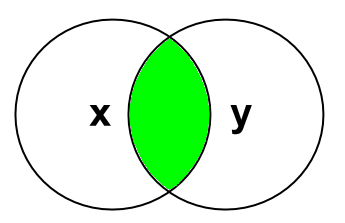
\includegraphics[width=2.3in]{images/inner_join}

\texttt{inner\_join(x,\ y)} only includes observations that match in
both x and y:

\begin{Shaded}
\begin{Highlighting}[]
\KeywordTok{inner_join}\NormalTok{(df1, df2)}
\end{Highlighting}
\end{Shaded}

\begin{verbatim}
## Joining, by = "id"
\end{verbatim}

\begin{verbatim}
##   id x1 x2
## 1  3  c  c
## 2  4  d  d
\end{verbatim}

\subsection{\texorpdfstring{\texttt{left\_join(x,\ y)}}{left\_join(x, y)}}\label{left_joinx-y}

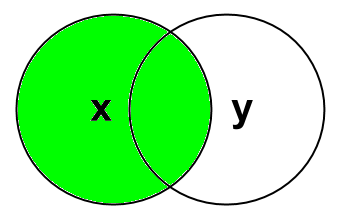
\includegraphics[width=2.26in]{images/left_join}

\texttt{left\_join(x,\ y)} includes all observations in \texttt{x},
regardless of whether they match or not. This is the most commonly used
join because it ensures that you don't lose observations from your
primary table:

\begin{Shaded}
\begin{Highlighting}[]
\KeywordTok{left_join}\NormalTok{(df1, df2)}
\end{Highlighting}
\end{Shaded}

\begin{verbatim}
## Joining, by = "id"
\end{verbatim}

\begin{verbatim}
##   id x1   x2
## 1  1  a <NA>
## 2  2  b <NA>
## 3  3  c    c
## 4  4  d    d
\end{verbatim}

\subsection{\texorpdfstring{\texttt{right\_join(x,\ y)}}{right\_join(x, y)}}\label{right_joinx-y}

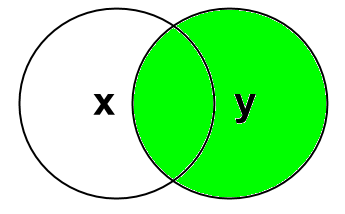
\includegraphics[width=2.3in]{images/right_join}

\texttt{right\_join(x,\ y)} includes all observations in \texttt{y}.
It's equivalent to \texttt{left\_join(y,\ x)}, but the columns will be
ordered differently:

\begin{Shaded}
\begin{Highlighting}[]
\KeywordTok{right_join}\NormalTok{(df1, df2)}
\end{Highlighting}
\end{Shaded}

\begin{verbatim}
## Joining, by = "id"
\end{verbatim}

\begin{verbatim}
##   id   x1 x2
## 1  3    c  c
## 2  4    d  d
## 3  5 <NA>  e
\end{verbatim}

\begin{Shaded}
\begin{Highlighting}[]
\KeywordTok{left_join}\NormalTok{(df2, df1)}
\end{Highlighting}
\end{Shaded}

\begin{verbatim}
## Joining, by = "id"
\end{verbatim}

\begin{verbatim}
##   id x2   x1
## 1  3  c    c
## 2  4  d    d
## 3  5  e <NA>
\end{verbatim}

\subsection{\texorpdfstring{\texttt{full\_join()}}{full\_join()}}\label{full_join}

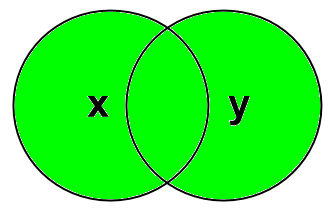
\includegraphics[width=2.23in]{images/full_join}

\texttt{full\_join()} includes all observations from \texttt{x} and
\texttt{y}:

\begin{Shaded}
\begin{Highlighting}[]
\KeywordTok{full_join}\NormalTok{(df1, df2)}
\end{Highlighting}
\end{Shaded}

\begin{verbatim}
## Joining, by = "id"
\end{verbatim}

\begin{verbatim}
##   id   x1   x2
## 1  1    a <NA>
## 2  2    b <NA>
## 3  3    c    c
## 4  4    d    d
## 5  5 <NA>    e
\end{verbatim}

The left, right and full joins are collectively know as outer joins.
When a row doesn't match in an outer join, the new variables are filled
in with missing values.

\clearpage

\section{dplyr with backend
databases}\label{dplyr-with-backend-databases}

\begin{Shaded}
\begin{Highlighting}[]
\KeywordTok{require}\NormalTok{(dplyr)}
\KeywordTok{require}\NormalTok{(ggplot2)}
\KeywordTok{require}\NormalTok{(DBI)}
\KeywordTok{require}\NormalTok{(RSQLite)}
\end{Highlighting}
\end{Shaded}

\subsection{Getting Started with Large
Data}\label{getting-started-with-large-data}

To experimement with large files you may want to use data from
\url{http://stat-computing.org/dataexpo/2009/the-data.html}.

The data consists of flight arrival and departure details for all
commercial flights within the USA, from October 1987 to April 2008. This
is a large dataset: there are nearly 120 million records in total, and
takes up 1.6 gigabytes of space compressed and 12Gb when uncompressed.
Only four of these files will be considered in the next example for a 29
millions records data frame.

This is clearly a case for SQLite: let us load the \texttt{RSQLite}
package.

\begin{Shaded}
\begin{Highlighting}[]
\KeywordTok{require}\NormalTok{(RSQLite)}
\end{Highlighting}
\end{Shaded}

As these files might have different encodings you may need to define a
simple function that returns the encoding of the file. Note that this
function uses unix system commands and may not work under windows based
computers.

\begin{Shaded}
\begin{Highlighting}[]
\NormalTok{charset <-}\StringTok{ }\NormalTok{function (file)\{}
  \NormalTok{info <-}\StringTok{ }\KeywordTok{system}\NormalTok{(}\KeywordTok{paste}\NormalTok{(}\StringTok{"file -i"} \NormalTok{,file ), }\DataTypeTok{intern =} \OtherTok{TRUE}\NormalTok{)}
  \NormalTok{info_split <-}\StringTok{ }\KeywordTok{strsplit}\NormalTok{(info, }\DataTypeTok{split =} \StringTok{"charset="}\NormalTok{)[[}\DecValTok{1}\NormalTok{]][}\DecValTok{2}\NormalTok{]}
  \NormalTok{info_split}
\NormalTok{\}}
\end{Highlighting}
\end{Shaded}

You then create an empty SQLite database with a little trick that
ensures the database is removed in case it already exists:

\begin{Shaded}
\begin{Highlighting}[]
\NormalTok{path <-}\StringTok{ "./"}
\NormalTok{db <-}\StringTok{ "ontime.sqlite"}
\NormalTok{path_db <-}\StringTok{ }\KeywordTok{paste}\NormalTok{(path, db, }\DataTypeTok{sep =} \StringTok{"/"}\NormalTok{)}
\NormalTok{db_exists <-}\StringTok{ }\KeywordTok{list.files}\NormalTok{(path, }\DataTypeTok{pattern =} \NormalTok{db)}
\NormalTok{if(}\KeywordTok{length}\NormalTok{(db_exists) !=}\StringTok{ }\DecValTok{0}\NormalTok{) }\KeywordTok{system}\NormalTok{(}\KeywordTok{paste}\NormalTok{(}\StringTok{"rm"}\NormalTok{, path_db))}
\NormalTok{con <-}\StringTok{ }\KeywordTok{dbConnect}\NormalTok{(RSQLite::}\KeywordTok{SQLite}\NormalTok{(), path_db)}
\end{Highlighting}
\end{Shaded}

Now it's time to get the list of files you want to load:

\begin{Shaded}
\begin{Highlighting}[]
\NormalTok{files <-}\StringTok{ }\KeywordTok{list.files}\NormalTok{(}\StringTok{"./../data"}\NormalTok{, }\DataTypeTok{pattern =} \StringTok{".csv"}\NormalTok{, }\DataTypeTok{full.names =} \OtherTok{TRUE}\NormalTok{)}
\end{Highlighting}
\end{Shaded}

and by using a for loop you can load all the files into the newly
created data base:

\begin{Shaded}
\begin{Highlighting}[]
\NormalTok{for (i in }\DecValTok{1}\NormalTok{:}\KeywordTok{length}\NormalTok{(files))\{}
  \NormalTok{head <-}\StringTok{ }\KeywordTok{ifelse} \NormalTok{(i ==}\StringTok{ }\DecValTok{1}\NormalTok{, }\OtherTok{TRUE}\NormalTok{, }\OtherTok{FALSE}\NormalTok{)}
  \NormalTok{skip <-}\StringTok{ }\KeywordTok{ifelse} \NormalTok{(i ==}\StringTok{ }\DecValTok{1}\NormalTok{, }\DecValTok{0}\NormalTok{, }\DecValTok{1}\NormalTok{)}
  \NormalTok{append <-}\StringTok{ }\KeywordTok{ifelse} \NormalTok{(i ==}\StringTok{ }\DecValTok{1}\NormalTok{, }\OtherTok{FALSE}\NormalTok{, }\OtherTok{TRUE}\NormalTok{)}
  \NormalTok{this_file <-}\StringTok{ }\NormalTok{files[i]}
  \NormalTok{encoding <-}\StringTok{ }\KeywordTok{charset}\NormalTok{(this_file)}
  \NormalTok{df <-}\StringTok{ }\KeywordTok{read.table}\NormalTok{(this_file, }\DataTypeTok{sep =} \StringTok{","}\NormalTok{, }\DataTypeTok{head =} \NormalTok{head, }\DataTypeTok{encoding =} \NormalTok{encoding, }\DataTypeTok{skip =} \NormalTok{skip, }\DataTypeTok{nrows =} \DecValTok{100}\NormalTok{)}
  \KeywordTok{dbWriteTable}\NormalTok{(}\DataTypeTok{conn =} \NormalTok{con, }\DataTypeTok{name =} \StringTok{"ontime"}\NormalTok{, }\DataTypeTok{value =} \NormalTok{df ,}\DataTypeTok{append =} \NormalTok{append)}
  \KeywordTok{cat}\NormalTok{(}\KeywordTok{date}\NormalTok{() , this_file, }\StringTok{"loaded"}\NormalTok{, }\StringTok{"}\CharTok{\textbackslash{}n}\StringTok{"}\NormalTok{)}
  \KeywordTok{rm}\NormalTok{(df)}
\NormalTok{\}  }
\end{Highlighting}
\end{Shaded}

finally disconnect from the database:

\begin{Shaded}
\begin{Highlighting}[]
\KeywordTok{dbDisconnect}\NormalTok{(con)}
\end{Highlighting}
\end{Shaded}

You can now start using the data base with dplyr interface:

\begin{Shaded}
\begin{Highlighting}[]
\NormalTok{con_dplyr <-}\StringTok{ }\KeywordTok{src_sqlite}\NormalTok{(path_db)}
\NormalTok{ontime <-}\StringTok{ }\KeywordTok{tbl}\NormalTok{(con_dplyr, }\StringTok{"ontime"}\NormalTok{)}
\KeywordTok{class}\NormalTok{(ontime)}
\KeywordTok{dim}\NormalTok{(ontime)}
\end{Highlighting}
\end{Shaded}

When working with databases, \texttt{dplyr} tries to be as lazy as
possible. It's lazy in two ways:

\begin{itemize}
\tightlist
\item
  It never pulls data back to \texttt{R} unless you explicitly ask for
  it;
\item
  It delays doing any work until the last possible minute, collecting
  together everything you want to do then sending that to the database
  in one step.
\end{itemize}

For example, take the following code:

\begin{Shaded}
\begin{Highlighting}[]
\NormalTok{ontime_stat <-}\StringTok{ }\NormalTok{ontime %>%}\StringTok{ }\KeywordTok{group_by}\NormalTok{(Year, Month) %>%}\StringTok{ }
\StringTok{   }\KeywordTok{summarise}\NormalTok{(}\DataTypeTok{avg =} \KeywordTok{mean}\NormalTok{(DepDelay), }\DataTypeTok{min =} \KeywordTok{min}\NormalTok{(DepDelay), }\DataTypeTok{max =} \KeywordTok{max}\NormalTok{(DepDelay)) }
\end{Highlighting}
\end{Shaded}

Suprisingly, this sequence of operations never actually touches the
database. It's not until you ask for the data (e.g.~by printing
\texttt{ontime\_stat}) that \texttt{dplyr} generates the SQL and
requests the results from the database, and even then it only pulls down
10 rows:

\begin{Shaded}
\begin{Highlighting}[]
\NormalTok{ontime_stat}
\KeywordTok{class}\NormalTok{(ontime_stat)}
\end{Highlighting}
\end{Shaded}

To pull down all the results use \texttt{collect()}, which returns a
\texttt{tbl} class object:

\begin{Shaded}
\begin{Highlighting}[]
\NormalTok{ontime_dep_delay <-}\StringTok{ }\NormalTok{ontime %>%}
\StringTok{  }\KeywordTok{select}\NormalTok{(}\DataTypeTok{year =} \NormalTok{Year, }\DataTypeTok{dep_delay =} \NormalTok{DepDelay, }\DataTypeTok{arr_delay =} \NormalTok{ArrDelay) %>%}
\StringTok{  }\KeywordTok{filter}\NormalTok{(dep_delay >}\StringTok{ }\DecValTok{0}\NormalTok{) %>%}
\StringTok{  }\KeywordTok{collect}\NormalTok{()}
\end{Highlighting}
\end{Shaded}

Once data are collected you can use it within \texttt{R}:

\begin{Shaded}
\begin{Highlighting}[]
\NormalTok{pl <-}\StringTok{ }\KeywordTok{ggplot}\NormalTok{(ontime_dep_delay , }\KeywordTok{aes}\NormalTok{(dep_delay, arr_delay))}
\NormalTok{pl <-}\StringTok{ }\NormalTok{pl +}\StringTok{ }\KeywordTok{stat_binhex}\NormalTok{(}\DataTypeTok{bins =} \DecValTok{30}\NormalTok{) +}\StringTok{ }\KeywordTok{facet_wrap}\NormalTok{(~year, }\DataTypeTok{ncol =} \DecValTok{2}\NormalTok{)}
\KeywordTok{print}\NormalTok{(pl)}
\end{Highlighting}
\end{Shaded}

\chapter{Reshaping data with tidyr}\label{reshaping-data-with-tidyr}

\begin{Shaded}
\begin{Highlighting}[]
\KeywordTok{require}\NormalTok{(dplyr)}
\KeywordTok{require}\NormalTok{(tidyr)}
\KeywordTok{require}\NormalTok{(qdata)}
\KeywordTok{require}\NormalTok{(ggplot2)}
\end{Highlighting}
\end{Shaded}

\section{Introduction}\label{introduction-1}

As a data scientist you collect data from different sources and, very
often you will have very little control on the original structure of
this data.

Such a variety in data structure implies long time spent at manipulating
your data prior any analysis or visualization step.

On the other hand, you may think about a well defined and standard way
storing your data so that data are ready to be pushed into any next
step.

This \emph{standard} format has been defined as \textbf{tidy}.

At the same time, analysis of visualization procedures require to be
ready to accept as input \emph{tidy} data structure. This is not always
the case but it is becoming more and more a standard in the \texttt{R}
community.

As a simple example let's consider the \texttt{people} data frame from
package \texttt{qdata}:

\begin{Shaded}
\begin{Highlighting}[]
\KeywordTok{data}\NormalTok{(people)}
\KeywordTok{head}\NormalTok{(people)}
\end{Highlighting}
\end{Shaded}

\begin{verbatim}
## # A tibble: 6 × 4
##   Gender   Area Weight Height
##   <fctr> <fctr>  <int>  <int>
## 1 Female  Isole     54    168
## 2 Female   Nord     61    171
## 3   Male    Sud     68    170
## 4 Female   Nord     52    164
## 5   Male   Nord     75    181
## 6   Male   Nord     77    178
\end{verbatim}

This data frame can be considered as a tidy data frame.

As a result, plotting \texttt{Weight} as a function of \texttt{Height}
with different colours for \texttt{Gender}, using package
\texttt{ggplot2}, is very straightforward as \texttt{ggplot2} is a set
of visualization tools ready for tidy data

\begin{Shaded}
\begin{Highlighting}[]
\KeywordTok{ggplot}\NormalTok{(people, }\KeywordTok{aes}\NormalTok{(}\DataTypeTok{x =} \NormalTok{Height, }\DataTypeTok{y =} \NormalTok{Weight, }\DataTypeTok{colour =} \NormalTok{Gender)) +}\StringTok{ }\KeywordTok{geom_point}\NormalTok{()}
\end{Highlighting}
\end{Shaded}

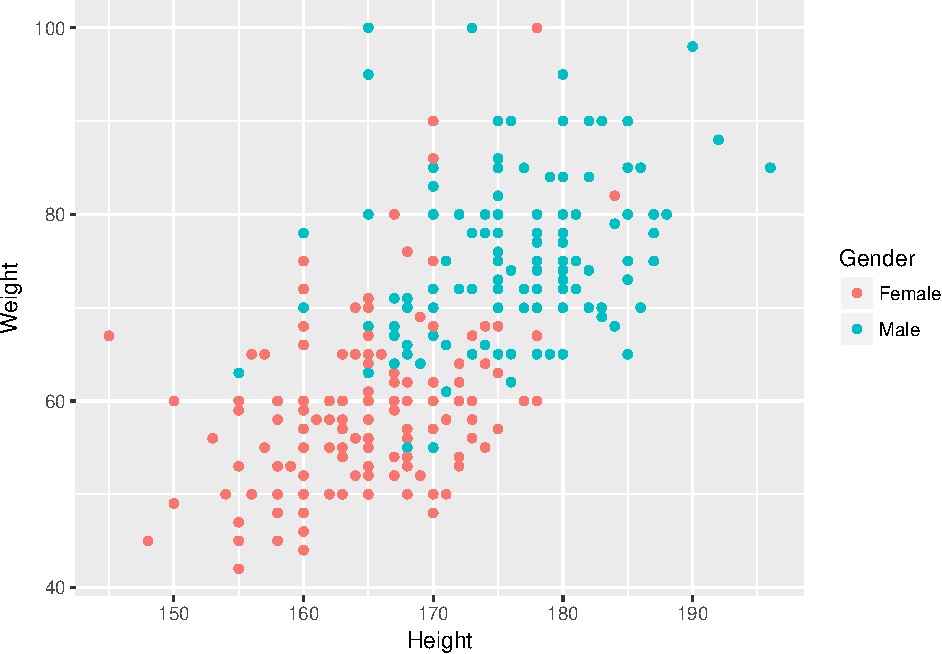
\includegraphics{46-tidyr_files/figure-latex/unnamed-chunk-2-1.pdf}

A similar result, with the standard \texttt{R} plotting tools, may
require first a data transformation effort:

\begin{Shaded}
\begin{Highlighting}[]
\NormalTok{female <-}\StringTok{ }\NormalTok{people[people$Gender ==}\StringTok{ 'Female'}\NormalTok{,]}
\NormalTok{male <-}\StringTok{ }\NormalTok{people[people$Gender ==}\StringTok{ 'Male'}\NormalTok{,]}
\end{Highlighting}
\end{Shaded}

followed by the plotting instruction:

\begin{Shaded}
\begin{Highlighting}[]
\KeywordTok{with}\NormalTok{(people, }\KeywordTok{plot}\NormalTok{(Height, Weight, }\DataTypeTok{type =} \StringTok{"n"}\NormalTok{))}
\KeywordTok{with}\NormalTok{(female, }\KeywordTok{points}\NormalTok{(Height, Weight, }\DataTypeTok{col =} \StringTok{"red"}\NormalTok{))}
\KeywordTok{with}\NormalTok{(male, }\KeywordTok{points}\NormalTok{(Height, Weight, }\DataTypeTok{col =} \StringTok{"blue"}\NormalTok{))    }
\end{Highlighting}
\end{Shaded}

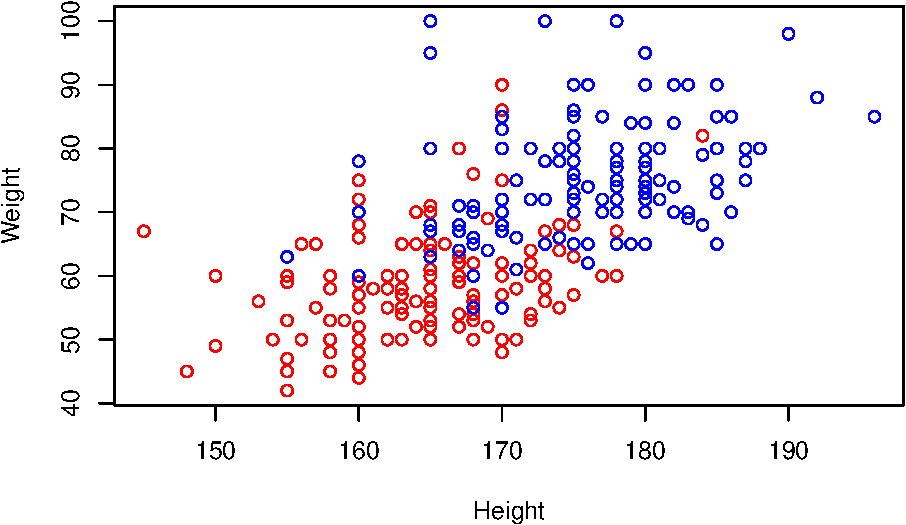
\includegraphics{46-tidyr_files/figure-latex/unnamed-chunk-4-1.pdf}

As a conclusion, as \emph{Hadley Wickam} writes: \emph{Tidy datasets and
tidy tools work hand in hand to make data analysis easier, allowing you
to focus on the interesting domain problem, not on the uninteresting
logistics of data.}

\section{Defining Tidy Data}\label{defining-tidy-data}

Tidy data is a standard way of mapping the meaning of a dataset to its
structure. A dataset is messy or tidy depending on how rows, columns and
tables are matched up with observations, variables and types.

In tidy data:

\begin{itemize}
\tightlist
\item
  each variable forms a column;
\item
  each observation forms a row;
\item
  each type of observational unit forms a table.
\end{itemize}

Tidy data makes it easy for an analyst or a computer to extract needed
variables because it provides a standard way of structuring a dataset.
Tidy data is particularly well suited for vectorized programming
languages like \texttt{R}, because the layout ensures that values of
different variables from the same observation are always paired.

\section{Tidying Messy Datasets}\label{tidying-messy-datasets}

Real datasets can, and often do, violate the three precepts of tidy data
in almost every way imaginable. These are the five most common problems
with messy datasets:

\begin{enumerate}
\def\labelenumi{\arabic{enumi}.}
\tightlist
\item
  column headers are values, not variable names;
\item
  multiple variables are stored in one column;
\item
  variables are stored in both rows and columns;
\item
  multiple types of observational units are stored in the same table;
\item
  a single observational unit is stored in multiple tables.
\end{enumerate}

\section{Tools}\label{tools}

Surprisingly, most messy datasets, including types of messiness not
explicitly described above, can be tidied with a small set of tools:

\begin{itemize}
\tightlist
\item
  \texttt{gather()} and \texttt{spread()}
\end{itemize}

\begin{figure}[htbp]
\centering
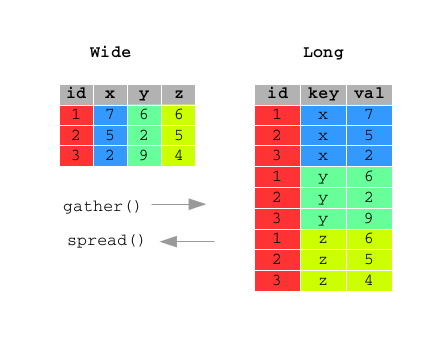
\includegraphics{images/gs.png}
\caption{}
\end{figure}

\clearpage

\begin{itemize}
\tightlist
\item
  \texttt{separate()} and \texttt{unite()}
\end{itemize}

\begin{figure}[htbp]
\centering
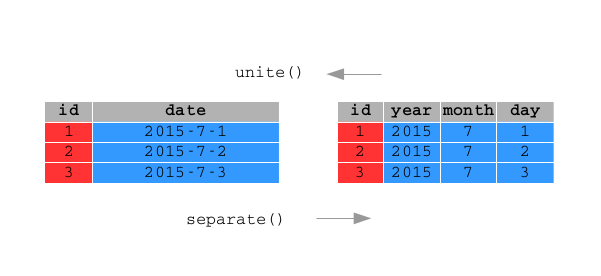
\includegraphics{images/us.png}
\caption{}
\end{figure}

\clearpage

\subsection{1. column headers are values, not variable
names}\label{column-headers-are-values-not-variable-names}

\begin{figure}[htbp]
\centering
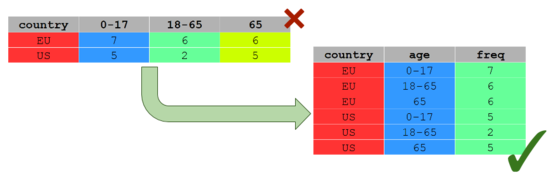
\includegraphics{images/tidy-case1.png}
\caption{}
\end{figure}

\begin{Shaded}
\begin{Highlighting}[]
\NormalTok{df <-}\StringTok{ }\KeywordTok{setNames}\NormalTok{(}\KeywordTok{data.frame}\NormalTok{(}\KeywordTok{c}\NormalTok{(}\StringTok{"EU"}\NormalTok{, }\StringTok{"US"}\NormalTok{), }\KeywordTok{c}\NormalTok{(}\DecValTok{7}\NormalTok{,}\DecValTok{5}\NormalTok{), }\KeywordTok{c}\NormalTok{(}\DecValTok{6}\NormalTok{,}\DecValTok{2}\NormalTok{), }\KeywordTok{c}\NormalTok{(}\DecValTok{6}\NormalTok{,}\DecValTok{5}\NormalTok{)),}
               \KeywordTok{c}\NormalTok{(}\StringTok{"country"}\NormalTok{,}\StringTok{"0-17"} \NormalTok{, }\StringTok{"18-65"}\NormalTok{, }\StringTok{"66+"}\NormalTok{))}

\NormalTok{df}
\end{Highlighting}
\end{Shaded}

\begin{verbatim}
##   country 0-17 18-65 66+
## 1      EU    7     6   6
## 2      US    5     2   5
\end{verbatim}

This data frame can be classified as \emph{messy} because variables:
\texttt{0-17}, \texttt{18-65}, \texttt{66+} are values of a variable,
say \texttt{age}, not column headers.

The unusual definition of column header by using function
\texttt{setNames()} is due to the non standard naming convention used in
this case. A syntactically valid name consists of letters, numbers and
the dot or underline characters and starts with a letter or the dot not
followed by a number.

The structure of \texttt{df} does not make clear:

\begin{itemize}
\tightlist
\item
  what column headers refer to
\item
  the meaning of each observational unit
\end{itemize}

A simple instruction to tidy this data is:

\begin{Shaded}
\begin{Highlighting}[]
\KeywordTok{gather}\NormalTok{(df, }\DataTypeTok{key =} \StringTok{"age"}\NormalTok{, }\DataTypeTok{value =} \StringTok{"freq"} \NormalTok{, }\DecValTok{2}\NormalTok{:}\DecValTok{4}\NormalTok{)}
\end{Highlighting}
\end{Shaded}

\begin{verbatim}
##   country   age freq
## 1      EU  0-17    7
## 2      US  0-17    5
## 3      EU 18-65    6
## 4      US 18-65    2
## 5      EU   66+    6
## 6      US   66+    5
\end{verbatim}

where \texttt{key} and \texttt{value} are the names for the newly
created key-value pair and \texttt{2:4} are the columns to stack. Again,
instead of passing the columns to stack by position it would be better
to use column names but, the unusual definition of column names does not
allow this.

\begin{Shaded}
\begin{Highlighting}[]
\NormalTok{df <-}\StringTok{ }\KeywordTok{data.frame}\NormalTok{(}\DataTypeTok{country =} \KeywordTok{c}\NormalTok{(}\StringTok{"EU"}\NormalTok{, }\StringTok{"US"}\NormalTok{),}
                \DataTypeTok{age_0_17 =} \KeywordTok{c}\NormalTok{(}\DecValTok{7}\NormalTok{,}\DecValTok{5}\NormalTok{), }
                \DataTypeTok{age_18_65 =} \KeywordTok{c}\NormalTok{(}\DecValTok{6}\NormalTok{,}\DecValTok{2}\NormalTok{), }
                \DataTypeTok{age_65 =} \KeywordTok{c}\NormalTok{(}\DecValTok{6}\NormalTok{,}\DecValTok{5}\NormalTok{))}
                
\NormalTok{df <-}\StringTok{ }\KeywordTok{gather}\NormalTok{(df, }\DataTypeTok{key =} \StringTok{"age"}\NormalTok{, }\DataTypeTok{value =} \StringTok{"freq"} \NormalTok{, age_0_17, age_18_65, age_65)}

\NormalTok{subx <-}\StringTok{ }\NormalTok{function(x, pattern, replacement , ...) }\KeywordTok{sub}\NormalTok{(pattern, replacement, x, ...)}

\NormalTok{df %>%}\StringTok{ }\KeywordTok{mutate}\NormalTok{(}\DataTypeTok{age =} \KeywordTok{subx}\NormalTok{(age, }\StringTok{"age_"}\NormalTok{, }\StringTok{""}\NormalTok{))}
\end{Highlighting}
\end{Shaded}

\begin{verbatim}
##   country   age freq
## 1      EU  0_17    7
## 2      US  0_17    5
## 3      EU 18_65    6
## 4      US 18_65    2
## 5      EU    65    6
## 6      US    65    5
\end{verbatim}

\clearpage

\subsection{2. multiple variables are stored in one
column}\label{multiple-variables-are-stored-in-one-column}

\begin{figure}[htbp]
\centering
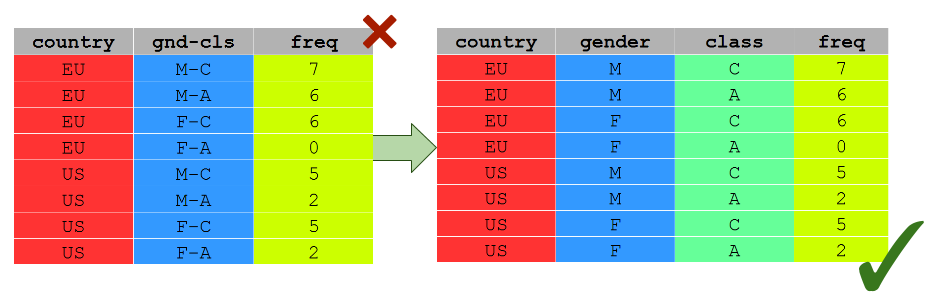
\includegraphics{images/tidy-case2.png}
\caption{}
\end{figure}

\begin{Shaded}
\begin{Highlighting}[]
\NormalTok{df <-}\StringTok{ }\KeywordTok{data.frame}\NormalTok{(}
  \DataTypeTok{country =} \KeywordTok{c}\NormalTok{(}\StringTok{"EU"}\NormalTok{, }\StringTok{"EU"}\NormalTok{, }\StringTok{"EU"}\NormalTok{, }\StringTok{"EU"}\NormalTok{, }\StringTok{"US"}\NormalTok{, }\StringTok{"US"}\NormalTok{, }\StringTok{"US"}\NormalTok{, }\StringTok{"US"}\NormalTok{),}
  \DataTypeTok{gnd_cls =} \KeywordTok{c}\NormalTok{(}\StringTok{"M-C"}\NormalTok{, }\StringTok{"M-A"}\NormalTok{, }\StringTok{"F-C"}\NormalTok{, }\StringTok{"F-A"}\NormalTok{, }\StringTok{"M-C"}\NormalTok{, }\StringTok{"M-A"}\NormalTok{, }\StringTok{"F-C"}\NormalTok{, }\StringTok{"F-A"}\NormalTok{),}
  \DataTypeTok{freq =} \KeywordTok{c}\NormalTok{(}\DecValTok{7}\NormalTok{,}\DecValTok{6}\NormalTok{,}\DecValTok{6}\NormalTok{,}\DecValTok{0}\NormalTok{,}\DecValTok{5}\NormalTok{,}\DecValTok{2}\NormalTok{,}\DecValTok{5}\NormalTok{,}\DecValTok{2}\NormalTok{))}

\NormalTok{df}
\end{Highlighting}
\end{Shaded}

\begin{verbatim}
##   country gnd_cls freq
## 1      EU     M-C    7
## 2      EU     M-A    6
## 3      EU     F-C    6
## 4      EU     F-A    0
## 5      US     M-C    5
## 6      US     M-A    2
## 7      US     F-C    5
## 8      US     F-A    2
\end{verbatim}

This data frame can be classified as messy because variable
\texttt{gnd\_cls} stores information about two variables:
\texttt{gender} and \texttt{class}.

Function \texttt{separate()}, whenever you can find a way to do it,
separate the content of a column into two columns:

\begin{Shaded}
\begin{Highlighting}[]
\KeywordTok{separate}\NormalTok{(df, }\DataTypeTok{col =} \StringTok{"gnd_cls"}\NormalTok{, }\DataTypeTok{into =} \KeywordTok{c}\NormalTok{(}\StringTok{"gender"}\NormalTok{, }\StringTok{"class"}\NormalTok{), }\DataTypeTok{sep =} \StringTok{"-"}\NormalTok{)}
\end{Highlighting}
\end{Shaded}

\begin{verbatim}
##   country gender class freq
## 1      EU      M     C    7
## 2      EU      M     A    6
## 3      EU      F     C    6
## 4      EU      F     A    0
## 5      US      M     C    5
## 6      US      M     A    2
## 7      US      F     C    5
## 8      US      F     A    2
\end{verbatim}

\clearpage

\subsection{3. variables are stored in both rows and
columns;}\label{variables-are-stored-in-both-rows-and-columns}

\begin{figure}[htbp]
\centering
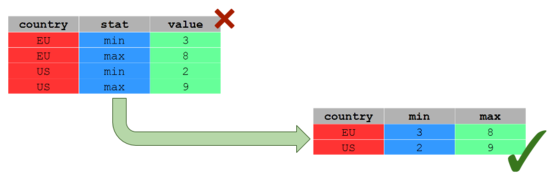
\includegraphics{images/tidy-case3.png}
\caption{}
\end{figure}

\begin{Shaded}
\begin{Highlighting}[]
\NormalTok{df <-}\StringTok{ }\KeywordTok{data.frame}\NormalTok{(}\DataTypeTok{country =} \KeywordTok{c}\NormalTok{(}\StringTok{"EU"}\NormalTok{, }\StringTok{"EU"}\NormalTok{, }\StringTok{"US"}\NormalTok{, }\StringTok{"US"}\NormalTok{),}
                 \DataTypeTok{stat =} \KeywordTok{c}\NormalTok{(}\StringTok{"min"}\NormalTok{, }\StringTok{"max"}\NormalTok{, }\StringTok{"min"}\NormalTok{, }\StringTok{"max"}\NormalTok{),}
                 \DataTypeTok{value =} \KeywordTok{c}\NormalTok{(}\DecValTok{3}\NormalTok{, }\DecValTok{8} \NormalTok{, }\DecValTok{2}\NormalTok{, }\DecValTok{9}\NormalTok{)}
                 \NormalTok{)}
\NormalTok{df}
\end{Highlighting}
\end{Shaded}

\begin{verbatim}
##   country stat value
## 1      EU  min     3
## 2      EU  max     8
## 3      US  min     2
## 4      US  max     9
\end{verbatim}

This data frame is \emph{messy} because observational units of variable
\texttt{stat} are variables by themselves.

Function \texttt{spread()} helps to structure this data in a tidy form:

\begin{Shaded}
\begin{Highlighting}[]
\KeywordTok{spread}\NormalTok{(df, }\DataTypeTok{key =} \NormalTok{stat, }\DataTypeTok{value =} \NormalTok{value)}
\end{Highlighting}
\end{Shaded}

\begin{verbatim}
##   country max min
## 1      EU   8   3
## 2      US   9   2
\end{verbatim}

\clearpage

\subsection{4. multiple types of observational units are stored in the
same
table}\label{multiple-types-of-observational-units-are-stored-in-the-same-table}

\begin{figure}[htbp]
\centering
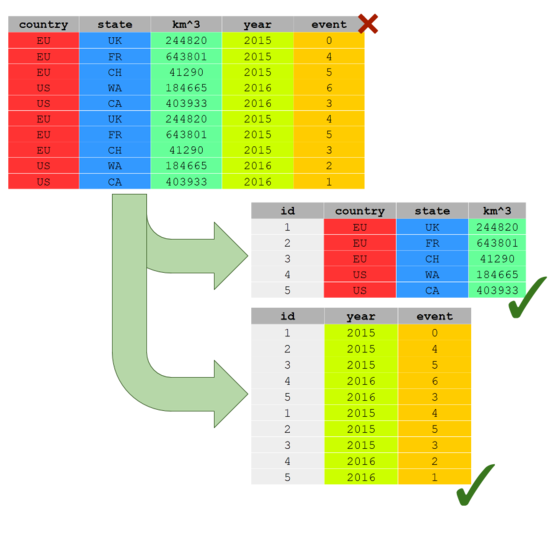
\includegraphics{images/tidy-case4.png}
\caption{}
\end{figure}

\begin{Shaded}
\begin{Highlighting}[]
\NormalTok{df <-}\StringTok{ }\KeywordTok{data.frame}\NormalTok{(}
  \DataTypeTok{country =}  \KeywordTok{c}\NormalTok{(}\StringTok{"EU"}\NormalTok{, }\StringTok{"EU"}\NormalTok{, }\StringTok{"EU"}\NormalTok{, }\StringTok{"US"}\NormalTok{, }\StringTok{"US"}\NormalTok{, }\StringTok{"EU"}\NormalTok{, }\StringTok{"EU"}\NormalTok{, }\StringTok{"EU"}\NormalTok{, }\StringTok{"US"}\NormalTok{, }\StringTok{"US"}\NormalTok{),}
  \DataTypeTok{state =} \KeywordTok{c}\NormalTok{(}\StringTok{"UK"}\NormalTok{, }\StringTok{"FR"}\NormalTok{, }\StringTok{"CH"}\NormalTok{, }\StringTok{"WA"}\NormalTok{, }\StringTok{"CA"}\NormalTok{,   }\StringTok{"UK"}\NormalTok{,   }\StringTok{"FR"}\NormalTok{,   }\StringTok{"CH"}\NormalTok{,   }\StringTok{"WA"}\NormalTok{,   }\StringTok{"CA"}\NormalTok{),}
  \DataTypeTok{km3 =} \KeywordTok{c}\NormalTok{(}\DecValTok{244820}\NormalTok{, }\DecValTok{643801}\NormalTok{, }\DecValTok{41290}\NormalTok{,    }\DecValTok{184665}\NormalTok{, }\DecValTok{403933}\NormalTok{, }\DecValTok{244820}\NormalTok{, }\DecValTok{643801}\NormalTok{, }\DecValTok{41290}\NormalTok{, }\DecValTok{184665}\NormalTok{, }\DecValTok{403933}\NormalTok{),}
  \DataTypeTok{year =} \KeywordTok{c}\NormalTok{(}\DecValTok{2015}\NormalTok{,    }\DecValTok{2015}\NormalTok{,   }\DecValTok{2015}\NormalTok{,   }\DecValTok{2016}\NormalTok{,   }\DecValTok{2016}\NormalTok{,   }\DecValTok{2015}\NormalTok{,   }\DecValTok{2015}\NormalTok{,   }\DecValTok{2015}\NormalTok{,   }\DecValTok{2016}\NormalTok{,   }\DecValTok{2016}\NormalTok{),}
  \DataTypeTok{event =} \KeywordTok{c}\NormalTok{(}\DecValTok{0}\NormalTok{, }\DecValTok{4}\NormalTok{,   }\DecValTok{5}\NormalTok{, }\DecValTok{6}\NormalTok{, }\DecValTok{3}\NormalTok{, }\DecValTok{4}\NormalTok{, }\DecValTok{5}\NormalTok{, }\DecValTok{3}\NormalTok{,   }\DecValTok{2}\NormalTok{, }\DecValTok{1}\NormalTok{))}

\NormalTok{df}
\end{Highlighting}
\end{Shaded}

\begin{verbatim}
##    country state    km3 year event
## 1       EU    UK 244820 2015     0
## 2       EU    FR 643801 2015     4
## 3       EU    CH  41290 2015     5
## 4       US    WA 184665 2016     6
## 5       US    CA 403933 2016     3
## 6       EU    UK 244820 2015     4
## 7       EU    FR 643801 2015     5
## 8       EU    CH  41290 2015     3
## 9       US    WA 184665 2016     2
## 10      US    CA 403933 2016     1
\end{verbatim}

This data frame stores two types of observational units in the same
table. Variables \texttt{country}, \texttt{state} and \texttt{km3} refer
to the first type of observational unit. The number of events:
\texttt{event} per year: \texttt{year} by \texttt{state} refer to a
second type of observational unit.

You can tidy this data by splitting the original data frame into two
data frame: \texttt{df1} and \texttt{df2}.

You first define \texttt{df1} by selecting the distinct values of the
type one columns:

\begin{Shaded}
\begin{Highlighting}[]
\NormalTok{df1 <-}\StringTok{  }\NormalTok{df %>%}\StringTok{ }
\StringTok{  }\KeywordTok{select}\NormalTok{(country, state, km3) %>%}\StringTok{ }
\StringTok{  }\KeywordTok{distinct}\NormalTok{()}
\NormalTok{df1 }
\end{Highlighting}
\end{Shaded}

\begin{verbatim}
##   country state    km3
## 1      EU    UK 244820
## 2      EU    FR 643801
## 3      EU    CH  41290
## 4      US    WA 184665
## 5      US    CA 403933
\end{verbatim}

After that you define \texttt{df2} as:

\begin{Shaded}
\begin{Highlighting}[]
\NormalTok{df2 <-}\StringTok{ }\NormalTok{df %>%}\StringTok{  }\KeywordTok{select}\NormalTok{(state, year, event)}
\end{Highlighting}
\end{Shaded}

\clearpage

\subsection{5. a single observational unit is stored in multiple
tables.}\label{a-single-observational-unit-is-stored-in-multiple-tables.}

\begin{figure}[htbp]
\centering
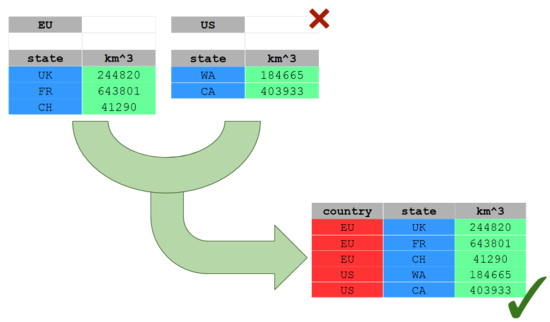
\includegraphics{images/tidy-case5.png}
\caption{}
\end{figure}

\begin{Shaded}
\begin{Highlighting}[]
\NormalTok{EU <-}\StringTok{ }\KeywordTok{data.frame}\NormalTok{(}\DataTypeTok{state =} \KeywordTok{c}\NormalTok{(}\StringTok{"UK"}\NormalTok{, }\StringTok{"FR"}\NormalTok{, }\StringTok{"CH"}\NormalTok{), }\DataTypeTok{km3 =} \KeywordTok{c}\NormalTok{(}\DecValTok{244820}\NormalTok{, }\DecValTok{643801}\NormalTok{, }\DecValTok{41290}\NormalTok{))}
\NormalTok{US <-}\StringTok{ }\KeywordTok{data.frame}\NormalTok{(}\DataTypeTok{state =} \KeywordTok{c}\NormalTok{(}\StringTok{"WA"}\NormalTok{, }\StringTok{"CA"}\NormalTok{), }\DataTypeTok{km3 =} \KeywordTok{c}\NormalTok{(}\DecValTok{184664}\NormalTok{, }\DecValTok{403933}\NormalTok{))}

\NormalTok{EU}
\end{Highlighting}
\end{Shaded}

\begin{verbatim}
##   state    km3
## 1    UK 244820
## 2    FR 643801
## 3    CH  41290
\end{verbatim}

\begin{Shaded}
\begin{Highlighting}[]
\NormalTok{US}
\end{Highlighting}
\end{Shaded}

\begin{verbatim}
##   state    km3
## 1    WA 184664
## 2    CA 403933
\end{verbatim}

This case often happens when you are loading data from different data
sources.

The name of the data frame, in this case, pays a crucial role as it has
to be stored into a variable:

Tidying this data requires more than one step:

First save the data frame name into a variable name:

\begin{Shaded}
\begin{Highlighting}[]
\NormalTok{EU <-}\StringTok{ }\NormalTok{EU %>%}\StringTok{ }\KeywordTok{mutate}\NormalTok{(}\DataTypeTok{country =} \StringTok{"EU"}\NormalTok{)}
\NormalTok{US <-}\StringTok{ }\NormalTok{US %>%}\StringTok{ }\KeywordTok{mutate}\NormalTok{(}\DataTypeTok{country =} \StringTok{"US"}\NormalTok{)}
\end{Highlighting}
\end{Shaded}

the combine by rows the two data frames

\begin{Shaded}
\begin{Highlighting}[]
\NormalTok{all <-}\StringTok{ }\KeywordTok{Reduce}\NormalTok{(rbind , }\KeywordTok{list}\NormalTok{(EU, US))}
\NormalTok{all}
\end{Highlighting}
\end{Shaded}

\begin{verbatim}
##   state    km3 country
## 1    UK 244820      EU
## 2    FR 643801      EU
## 3    CH  41290      EU
## 4    WA 184664      US
## 5    CA 403933      US
\end{verbatim}

\section{Example: Phone Time}\label{example-phone-time}

In this example about some measurements of how much time people spend on
their phones, measured at two locations (work and home), at two times.
Each person has been randomly assigned to either treatment or control.

\begin{Shaded}
\begin{Highlighting}[]
\NormalTok{messy <-}\StringTok{ }\KeywordTok{data.frame}\NormalTok{(}
  \DataTypeTok{id =} \DecValTok{1}\NormalTok{:}\DecValTok{4}\NormalTok{,}
  \DataTypeTok{trt =} \KeywordTok{rep}\NormalTok{(}\KeywordTok{c}\NormalTok{(}\StringTok{'control'}\NormalTok{, }\StringTok{'treatment'}\NormalTok{), }\DataTypeTok{each =} \DecValTok{2}\NormalTok{),}
  \DataTypeTok{work.T1 =} \KeywordTok{c}\NormalTok{(}\DecValTok{7}\NormalTok{, }\DecValTok{6}\NormalTok{, }\DecValTok{4}\NormalTok{, }\DecValTok{3}\NormalTok{),}
  \DataTypeTok{home.T1 =} \KeywordTok{c}\NormalTok{(}\DecValTok{5}\NormalTok{, }\DecValTok{4}\NormalTok{, }\DecValTok{1}\NormalTok{, }\DecValTok{3}\NormalTok{),}
  \DataTypeTok{work.T2 =} \KeywordTok{c}\NormalTok{(}\DecValTok{22}\NormalTok{, }\DecValTok{27}\NormalTok{, }\DecValTok{20}\NormalTok{, }\DecValTok{16}\NormalTok{),}
  \DataTypeTok{home.T2 =} \KeywordTok{c}\NormalTok{(}\DecValTok{11}\NormalTok{, }\DecValTok{7}\NormalTok{, }\DecValTok{10}\NormalTok{, }\DecValTok{6}\NormalTok{)}
\NormalTok{)}
\NormalTok{messy}
\end{Highlighting}
\end{Shaded}

\begin{verbatim}
##   id       trt work.T1 home.T1 work.T2 home.T2
## 1  1   control       7       5      22      11
## 2  2   control       6       4      27       7
## 3  3 treatment       4       1      20      10
## 4  4 treatment       3       3      16       6
\end{verbatim}

To tidy this data, before using \texttt{gather()} it is necessary to
turn columns \texttt{work.T1}, \texttt{home.T1}, \texttt{work.T2} and
\texttt{home.T2} into a key-value pair of key and time.

\begin{Shaded}
\begin{Highlighting}[]
\NormalTok{tidier <-}\StringTok{ }\KeywordTok{gather}\NormalTok{(messy, key, time, -id, -trt)}
\NormalTok{tidier}
\end{Highlighting}
\end{Shaded}

\begin{verbatim}
##    id       trt     key time
## 1   1   control work.T1    7
## 2   2   control work.T1    6
## 3   3 treatment work.T1    4
## 4   4 treatment work.T1    3
## 5   1   control home.T1    5
## 6   2   control home.T1    4
## 7   3 treatment home.T1    1
## 8   4 treatment home.T1    3
## 9   1   control work.T2   22
## 10  2   control work.T2   27
## 11  3 treatment work.T2   20
## 12  4 treatment work.T2   16
## 13  1   control home.T2   11
## 14  2   control home.T2    7
## 15  3 treatment home.T2   10
## 16  4 treatment home.T2    6
\end{verbatim}

Next \texttt{separate()} splits the key into \texttt{location} and
\texttt{time}, using a regular expression to describe the character that
separates them.

\begin{Shaded}
\begin{Highlighting}[]
\NormalTok{tidy <-}\StringTok{ }\KeywordTok{separate}\NormalTok{(tidier, }\DataTypeTok{col =} \NormalTok{key, }\DataTypeTok{into =} \KeywordTok{c}\NormalTok{(}\StringTok{"location"}\NormalTok{, }\StringTok{"time"}\NormalTok{), }\DataTypeTok{sep =} \StringTok{"}\CharTok{\textbackslash{}\textbackslash{}}\StringTok{."}\NormalTok{)}
\NormalTok{tidy}
\end{Highlighting}
\end{Shaded}

\begin{verbatim}
##    id       trt location time time
## 1   1   control     work   T1    7
## 2   2   control     work   T1    6
## 3   3 treatment     work   T1    4
## 4   4 treatment     work   T1    3
## 5   1   control     home   T1    5
## 6   2   control     home   T1    4
## 7   3 treatment     home   T1    1
## 8   4 treatment     home   T1    3
## 9   1   control     work   T2   22
## 10  2   control     work   T2   27
## 11  3 treatment     work   T2   20
## 12  4 treatment     work   T2   16
## 13  1   control     home   T2   11
## 14  2   control     home   T2    7
## 15  3 treatment     home   T2   10
## 16  4 treatment     home   T2    6
\end{verbatim}

\section{Example: Stock Market data}\label{example-stock-market-data}

Supposing you have the following packages, load them into \texttt{R}:

\begin{Shaded}
\begin{Highlighting}[]
\KeywordTok{require}\NormalTok{(quantmod)}
\KeywordTok{require}\NormalTok{(lubridate)}
\end{Highlighting}
\end{Shaded}

Then, download these data from Google Finance:

\begin{Shaded}
\begin{Highlighting}[]
\KeywordTok{invisible}\NormalTok{(}\KeywordTok{Sys.setlocale}\NormalTok{(}\StringTok{"LC_MESSAGES"}\NormalTok{, }\StringTok{"C"}\NormalTok{))}
\KeywordTok{invisible}\NormalTok{(}\KeywordTok{Sys.setlocale}\NormalTok{(}\StringTok{"LC_TIME"}\NormalTok{, }\StringTok{"C"}\NormalTok{))}
\KeywordTok{getSymbols.google}\NormalTok{(}\DataTypeTok{Symbols =} \StringTok{"IBM"}\NormalTok{,}
                  \DataTypeTok{env =} \KeywordTok{globalenv}\NormalTok{(),}
                  \DataTypeTok{return.class =} \StringTok{'data.frame'}\NormalTok{,}
                  \DataTypeTok{from =} \StringTok{"2015-01-01"}\NormalTok{,}
                  \DataTypeTok{to =} \KeywordTok{Sys.Date}\NormalTok{())}
\end{Highlighting}
\end{Shaded}

\begin{verbatim}
## [1] "IBM"
\end{verbatim}

\begin{Shaded}
\begin{Highlighting}[]
\KeywordTok{head}\NormalTok{(IBM)}
\end{Highlighting}
\end{Shaded}

\begin{verbatim}
##            IBM.Open IBM.High IBM.Low IBM.Close IBM.Volume
## 2015-01-02   161.31   163.31  161.00    162.06    5525466
## 2015-01-05   161.27   161.27  159.19    159.51    4880389
## 2015-01-06   159.67   159.96  155.17    156.07    6146712
## 2015-01-07   157.20   157.20  154.03    155.05    4701839
## 2015-01-08   156.24   159.04  155.55    158.42    4241113
## 2015-01-09   158.42   160.34  157.25    159.11    4488347
\end{verbatim}

In the following code chunks you will find also some \texttt{dplyr}
functions. To better understand them, see the next chapters of the
course, in particular the \texttt{dplyr} parts about \texttt{mutate()}
and \texttt{summarise()}.

Manipulate data from wide to long:

\begin{Shaded}
\begin{Highlighting}[]
\NormalTok{df  <-}\StringTok{ }\NormalTok{IBM  %>%}\StringTok{ }
\StringTok{  }\KeywordTok{transmute}\NormalTok{(}\DataTypeTok{time =} \KeywordTok{ymd}\NormalTok{(}\KeywordTok{row.names}\NormalTok{(.)), }\DataTypeTok{open =} \NormalTok{IBM.Open, }\DataTypeTok{high =} \NormalTok{IBM.High, }\DataTypeTok{low =} \NormalTok{IBM.Low, }
            \DataTypeTok{close =} \NormalTok{IBM.Close) %>%}
\StringTok{  }\KeywordTok{gather}\NormalTok{(}\DataTypeTok{key =} \NormalTok{hloc, }\DataTypeTok{value =} \NormalTok{price, -time) %>%}
\StringTok{  }\KeywordTok{mutate}\NormalTok{(}\DataTypeTok{hloc =} \KeywordTok{factor}\NormalTok{(hloc)) %>%}
\StringTok{  }\KeywordTok{tbl_df}\NormalTok{()}
\KeywordTok{head}\NormalTok{(df)}
\end{Highlighting}
\end{Shaded}

\begin{verbatim}
## # A tibble: 6 × 3
##         time   hloc  price
##       <date> <fctr>  <dbl>
## 1 2015-01-02   open 161.31
## 2 2015-01-05   open 161.27
## 3 2015-01-06   open 159.67
## 4 2015-01-07   open 157.20
## 5 2015-01-08   open 156.24
## 6 2015-01-09   open 158.42
\end{verbatim}

Plot data with ggplot:

\begin{Shaded}
\begin{Highlighting}[]
\KeywordTok{ggplot}\NormalTok{(}\DataTypeTok{data =} \NormalTok{df, }\KeywordTok{aes}\NormalTok{(}\DataTypeTok{x =} \NormalTok{time, }\DataTypeTok{y =} \NormalTok{price, }\DataTypeTok{colour =} \NormalTok{hloc)) +}\StringTok{ }\KeywordTok{geom_line}\NormalTok{() }
\end{Highlighting}
\end{Shaded}

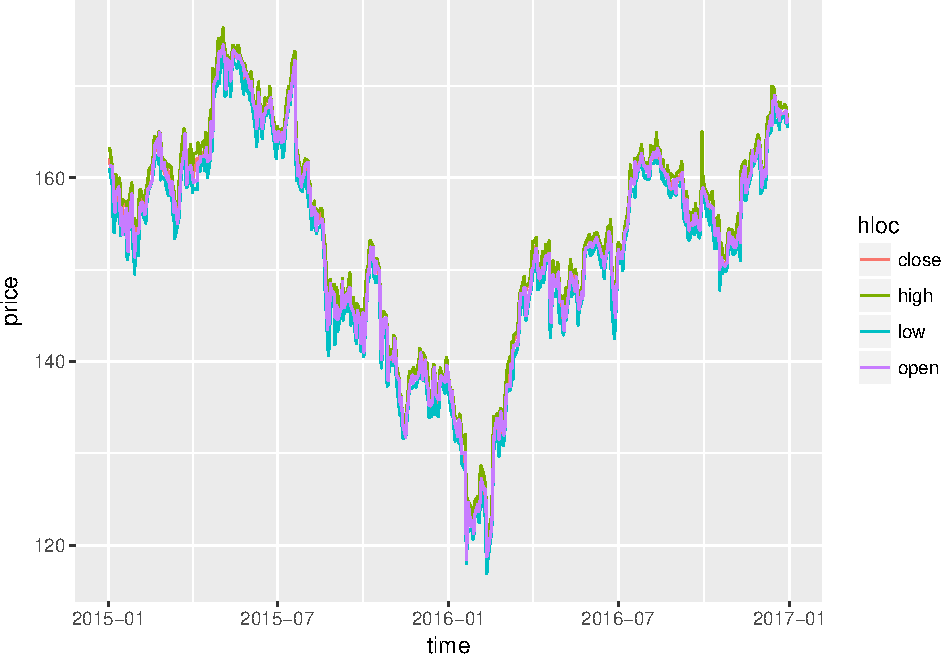
\includegraphics{46-tidyr_files/figure-latex/unnamed-chunk-24-1.pdf}

Compute returns:

\begin{Shaded}
\begin{Highlighting}[]
\NormalTok{df <-}\StringTok{ }\NormalTok{df %>%}\StringTok{ }\KeywordTok{group_by}\NormalTok{(hloc) %>%}\StringTok{ }\KeywordTok{mutate}\NormalTok{(}\DataTypeTok{returns =} \NormalTok{(price -}\StringTok{ }\KeywordTok{lag}\NormalTok{(price))/}\KeywordTok{lag}\NormalTok{(price))}
\KeywordTok{head}\NormalTok{(df)}
\end{Highlighting}
\end{Shaded}

\begin{verbatim}
## Source: local data frame [6 x 4]
## Groups: hloc [1]
## 
##         time   hloc  price       returns
##       <date> <fctr>  <dbl>         <dbl>
## 1 2015-01-02   open 161.31            NA
## 2 2015-01-05   open 161.27 -0.0002479697
## 3 2015-01-06   open 159.67 -0.0099212501
## 4 2015-01-07   open 157.20 -0.0154694056
## 5 2015-01-08   open 156.24 -0.0061068702
## 6 2015-01-09   open 158.42  0.0139528930
\end{verbatim}

And summarise them:

\begin{Shaded}
\begin{Highlighting}[]
\NormalTok{df %>%}
\StringTok{  }\KeywordTok{group_by}\NormalTok{(hloc) %>%}
\StringTok{  }\KeywordTok{summarise}\NormalTok{(}\DataTypeTok{n =} \KeywordTok{n}\NormalTok{(), }\DataTypeTok{avg =} \KeywordTok{mean}\NormalTok{(returns, }\DataTypeTok{na.rm =} \OtherTok{TRUE}\NormalTok{), }\DataTypeTok{sd =} \KeywordTok{sd}\NormalTok{(returns, }\DataTypeTok{na.rm =} \OtherTok{TRUE}\NormalTok{))}
\end{Highlighting}
\end{Shaded}

\begin{verbatim}
## # A tibble: 4 × 4
##     hloc     n          avg         sd
##   <fctr> <int>        <dbl>      <dbl>
## 1  close   509 0.0001504396 0.01291350
## 2   high   509 0.0001410029 0.01133475
## 3    low   509 0.0001568441 0.01240202
## 4   open   509 0.0001752224 0.01244935
\end{verbatim}

\chapter{Managing dates with
lubridate}\label{managing-dates-with-lubridate}

\begin{Shaded}
\begin{Highlighting}[]
\KeywordTok{require}\NormalTok{(lubridate)}
\KeywordTok{require}\NormalTok{(dplyr)}
\KeywordTok{require}\NormalTok{(ggplot2)}
\KeywordTok{require}\NormalTok{(tidyr)}
\KeywordTok{require}\NormalTok{(qdata)}
\end{Highlighting}
\end{Shaded}

\section{\texorpdfstring{A First Look to
\texttt{lubridate}}{A First Look to lubridate}}\label{a-first-look-to-lubridate}

Among packages that deals with dates and times in R, \texttt{lubridate}
provides a set of intuitive and coherent functions. Intuitive since each
function usually perform a single task described by its name; coherent
since \texttt{lubridate} is well integrated with other data management
tools, like \texttt{dplyr}.

Supposing \texttt{lubridate} is currently installed, it must be loaded
in order to use its functions.

\begin{Shaded}
\begin{Highlighting}[]
\KeywordTok{require}\NormalTok{(lubridate)}
\end{Highlighting}
\end{Shaded}

The starting point is a character string.

\begin{Shaded}
\begin{Highlighting}[]
\NormalTok{chr <-}\StringTok{ "01-02-12"}
\KeywordTok{class}\NormalTok{(chr)}
\end{Highlighting}
\end{Shaded}

\begin{verbatim}
## [1] "character"
\end{verbatim}

The above string is an ambiguous date:

\begin{itemize}
\tightlist
\item
  in Europe, it can be easily interpreted as 1st February 2012,
\item
  in the US, it can be read as January 2, 2012,
\item
  IT developers write in this way the day 12 February 2001.
\end{itemize}

\texttt{lubridate} provides a single function for each one of these
cases: \texttt{dmy()}, \texttt{mdy()} and \texttt{ymd()}. These
functions parse dates according to the order provided, where \texttt{y}
is the \emph{year}, \texttt{m} is the \emph{month} and \texttt{d} is the
\emph{day}.

\begin{Shaded}
\begin{Highlighting}[]
\KeywordTok{dmy}\NormalTok{(chr)}
\end{Highlighting}
\end{Shaded}

\begin{verbatim}
## [1] "2012-02-01"
\end{verbatim}

\begin{Shaded}
\begin{Highlighting}[]
\KeywordTok{mdy}\NormalTok{(chr)}
\end{Highlighting}
\end{Shaded}

\begin{verbatim}
## [1] "2012-01-02"
\end{verbatim}

\begin{Shaded}
\begin{Highlighting}[]
\KeywordTok{ymd}\NormalTok{(chr)}
\end{Highlighting}
\end{Shaded}

\begin{verbatim}
## [1] "2001-02-12"
\end{verbatim}

\begin{Shaded}
\begin{Highlighting}[]
\KeywordTok{class}\NormalTok{(}\KeywordTok{dmy}\NormalTok{(chr))}
\end{Highlighting}
\end{Shaded}

\begin{verbatim}
## [1] "Date"
\end{verbatim}

Parsed objects have now two new classes: \texttt{POSIXct} and
\texttt{POSIXt}. As Wikipedia states, \emph{the Portable Operating
System Interface (POSIX) is a family of standards specified by the IEEE
Computer Society for maintaining compatibility between operating
systems}.

The \texttt{POSIXct} format stores dates as the number of seconds since
the start of January 1, 1970, as shown by \texttt{as.numeric()} below;
\texttt{POSIXt} is a virtual class common to \texttt{POSIXct} and other
\texttt{POSIX*} classes that are not used here.

\begin{Shaded}
\begin{Highlighting}[]
\KeywordTok{as.numeric}\NormalTok{(}\KeywordTok{dmy}\NormalTok{(chr))}
\end{Highlighting}
\end{Shaded}

\begin{verbatim}
## [1] 15371
\end{verbatim}

The \texttt{lubridate} package provides other parsing functions, to deal
with less frequent cases \texttt{myd()}, \texttt{dym()} and
\texttt{ydm()}.

\begin{Shaded}
\begin{Highlighting}[]
\KeywordTok{myd}\NormalTok{(chr)}
\end{Highlighting}
\end{Shaded}

\begin{verbatim}
## [1] "2002-01-12"
\end{verbatim}

\begin{Shaded}
\begin{Highlighting}[]
\KeywordTok{dym}\NormalTok{(chr)}
\end{Highlighting}
\end{Shaded}

\begin{verbatim}
## [1] "2002-12-01"
\end{verbatim}

\begin{Shaded}
\begin{Highlighting}[]
\KeywordTok{ydm}\NormalTok{(chr)}
\end{Highlighting}
\end{Shaded}

\begin{verbatim}
## [1] "2001-12-02"
\end{verbatim}

Accordingly to the help, \texttt{ymd()}-style \emph{functions recognize
arbitrary non-digit separators as well as no separator. As long as the
order of formats is correct, these functions will parse dates correctly
even when the input vectors contain differently formatted dates}.

\begin{Shaded}
\begin{Highlighting}[]
\NormalTok{x <-}\StringTok{ }\KeywordTok{c}\NormalTok{(}\DecValTok{20160101}\NormalTok{, }\StringTok{"2016-01-02"}\NormalTok{, }\StringTok{"2016 01 03"}\NormalTok{, }\StringTok{"2016-1-4"}\NormalTok{, }\StringTok{"2016-1, 5"}\NormalTok{, }
       \StringTok{"Created on 2016 1 6"}\NormalTok{, }\StringTok{"201601 !!! 07"}\NormalTok{)}
\KeywordTok{ymd}\NormalTok{(x)}
\end{Highlighting}
\end{Shaded}

\begin{verbatim}
## [1] "2016-01-01" "2016-01-02" "2016-01-03" "2016-01-04" "2016-01-05" "2016-01-06" "2016-01-07"
\end{verbatim}

\section{Extract Date Components}\label{extract-date-components}

The following function returns an \texttt{IBM} data frame with IBM
quotation data from Yahoo! Finance. Notice that the function refer to
the \texttt{quantmod} package, so it should be installed.

\begin{Shaded}
\begin{Highlighting}[]
\NormalTok{quantmod::}\KeywordTok{getSymbols}\NormalTok{(}\StringTok{"IBM"}\NormalTok{, }\DataTypeTok{return.class =} \StringTok{'data.frame'}\NormalTok{)}
\end{Highlighting}
\end{Shaded}

\begin{verbatim}
## [1] "IBM"
\end{verbatim}

\begin{Shaded}
\begin{Highlighting}[]
\KeywordTok{head}\NormalTok{(IBM)}
\end{Highlighting}
\end{Shaded}

\begin{verbatim}
##            IBM.Open IBM.High IBM.Low IBM.Close IBM.Volume IBM.Adjusted
## 2007-01-03    97.18    98.40   96.26     97.27    9196800     78.35465
## 2007-01-04    97.25    98.79   96.88     98.31   10524500     79.19241
## 2007-01-05    97.60    97.95   96.91     97.42    7221300     78.47548
## 2007-01-08    98.50    99.50   98.35     98.90   10340000     79.66768
## 2007-01-09    99.08   100.33   99.07    100.07   11108200     80.61016
## 2007-01-10    98.50    99.05   97.93     98.89    8744800     79.65962
\end{verbatim}

The data frame contains dates as row names but data manipulation can be
performed better on a variable. With a bit of \texttt{dplyr} code the
new column can be added.

\begin{Shaded}
\begin{Highlighting}[]
\NormalTok{IBM <-}\StringTok{ }\NormalTok{IBM %>%}\StringTok{ }\KeywordTok{mutate}\NormalTok{(}\DataTypeTok{date =} \KeywordTok{row.names}\NormalTok{(.)) %>%}\StringTok{ }\NormalTok{tbl_df }
\NormalTok{IBM}
\end{Highlighting}
\end{Shaded}

\begin{verbatim}
## # A tibble: 2,523 × 7
##    IBM.Open IBM.High IBM.Low IBM.Close IBM.Volume IBM.Adjusted       date
##       <dbl>    <dbl>   <dbl>     <dbl>      <dbl>        <dbl>      <chr>
## 1     97.18    98.40   96.26     97.27    9196800     78.35465 2007-01-03
## 2     97.25    98.79   96.88     98.31   10524500     79.19241 2007-01-04
## 3     97.60    97.95   96.91     97.42    7221300     78.47548 2007-01-05
## 4     98.50    99.50   98.35     98.90   10340000     79.66768 2007-01-08
## 5     99.08   100.33   99.07    100.07   11108200     80.61016 2007-01-09
## 6     98.50    99.05   97.93     98.89    8744800     79.65962 2007-01-10
## 7     99.00    99.90   98.50     98.65    8000700     79.46630 2007-01-11
## 8     98.99    99.69   98.50     99.34    6636500     80.02211 2007-01-12
## 9     99.40   100.84   99.30    100.82    9602200     81.21431 2007-01-16
## 10   100.69   100.90   99.90    100.02    8200700     80.56988 2007-01-17
## # ... with 2,513 more rows
\end{verbatim}

At this point, the new \texttt{date} column is a string and it must be
parsed to be interpreted by R as a date.

\begin{Shaded}
\begin{Highlighting}[]
\NormalTok{IBM <-}\StringTok{ }\NormalTok{IBM %>%}\StringTok{ }\KeywordTok{mutate}\NormalTok{(}\DataTypeTok{date =} \KeywordTok{ymd}\NormalTok{(date))}
\NormalTok{IBM}
\end{Highlighting}
\end{Shaded}

\begin{verbatim}
## # A tibble: 2,523 × 7
##    IBM.Open IBM.High IBM.Low IBM.Close IBM.Volume IBM.Adjusted       date
##       <dbl>    <dbl>   <dbl>     <dbl>      <dbl>        <dbl>     <date>
## 1     97.18    98.40   96.26     97.27    9196800     78.35465 2007-01-03
## 2     97.25    98.79   96.88     98.31   10524500     79.19241 2007-01-04
## 3     97.60    97.95   96.91     97.42    7221300     78.47548 2007-01-05
## 4     98.50    99.50   98.35     98.90   10340000     79.66768 2007-01-08
## 5     99.08   100.33   99.07    100.07   11108200     80.61016 2007-01-09
## 6     98.50    99.05   97.93     98.89    8744800     79.65962 2007-01-10
## 7     99.00    99.90   98.50     98.65    8000700     79.46630 2007-01-11
## 8     98.99    99.69   98.50     99.34    6636500     80.02211 2007-01-12
## 9     99.40   100.84   99.30    100.82    9602200     81.21431 2007-01-16
## 10   100.69   100.90   99.90    100.02    8200700     80.56988 2007-01-17
## # ... with 2,513 more rows
\end{verbatim}

The \texttt{lubridate} package provide a set of function to extract
single components of a date: \texttt{month()}, \texttt{day()} and
\texttt{year()}. Using just \texttt{lubridate} and \texttt{dplyr} the
components of a date can be added as new variables to a data frame.

\begin{Shaded}
\begin{Highlighting}[]
\NormalTok{IBM <-}\StringTok{ }\NormalTok{IBM %>%}\StringTok{ }\KeywordTok{mutate}\NormalTok{(}\DataTypeTok{month =} \KeywordTok{month}\NormalTok{(date), }\DataTypeTok{day =} \KeywordTok{day}\NormalTok{(date), }\DataTypeTok{year =} \KeywordTok{year}\NormalTok{(date))}
\NormalTok{IBM}
\end{Highlighting}
\end{Shaded}

\begin{verbatim}
## # A tibble: 2,523 × 10
##    IBM.Open IBM.High IBM.Low IBM.Close IBM.Volume IBM.Adjusted       date month   day  year
##       <dbl>    <dbl>   <dbl>     <dbl>      <dbl>        <dbl>     <date> <dbl> <int> <dbl>
## 1     97.18    98.40   96.26     97.27    9196800     78.35465 2007-01-03     1     3  2007
## 2     97.25    98.79   96.88     98.31   10524500     79.19241 2007-01-04     1     4  2007
## 3     97.60    97.95   96.91     97.42    7221300     78.47548 2007-01-05     1     5  2007
## 4     98.50    99.50   98.35     98.90   10340000     79.66768 2007-01-08     1     8  2007
## 5     99.08   100.33   99.07    100.07   11108200     80.61016 2007-01-09     1     9  2007
## 6     98.50    99.05   97.93     98.89    8744800     79.65962 2007-01-10     1    10  2007
## 7     99.00    99.90   98.50     98.65    8000700     79.46630 2007-01-11     1    11  2007
## 8     98.99    99.69   98.50     99.34    6636500     80.02211 2007-01-12     1    12  2007
## 9     99.40   100.84   99.30    100.82    9602200     81.21431 2007-01-16     1    16  2007
## 10   100.69   100.90   99.90    100.02    8200700     80.56988 2007-01-17     1    17  2007
## # ... with 2,513 more rows
\end{verbatim}

At this point, you can easily draw a time series plot with adjusted
quotations for the IBM, with a facet for each year.

\begin{Shaded}
\begin{Highlighting}[]
\KeywordTok{ggplot}\NormalTok{(}\DataTypeTok{data=}\NormalTok{IBM, }\DataTypeTok{mapping=}\KeywordTok{aes}\NormalTok{(}\DataTypeTok{x=}\NormalTok{date)) +}
\StringTok{  }\KeywordTok{geom_line}\NormalTok{(}\KeywordTok{aes}\NormalTok{(}\DataTypeTok{y=}\NormalTok{IBM.Adjusted)) +}\StringTok{ }
\StringTok{  }\KeywordTok{facet_wrap}\NormalTok{(~}\StringTok{ }\NormalTok{year, }\DataTypeTok{scales=}\StringTok{"free_x"}\NormalTok{)}
\end{Highlighting}
\end{Shaded}

\includegraphics{47-lubridate_files/figure-latex/lubridate_ggp_facets-1.pdf}

Similarly, you can explore differences among months with a box plot for
each month.

\begin{Shaded}
\begin{Highlighting}[]
\KeywordTok{ggplot}\NormalTok{(}\DataTypeTok{data=}\NormalTok{IBM, }\DataTypeTok{mapping=}\KeywordTok{aes}\NormalTok{(}\DataTypeTok{x=}\KeywordTok{factor}\NormalTok{(month), }\DataTypeTok{y=}\NormalTok{IBM.Adjusted, }\DataTypeTok{group=}\NormalTok{month)) +}
\StringTok{  }\KeywordTok{geom_boxplot}\NormalTok{() +}
\StringTok{  }\KeywordTok{facet_wrap}\NormalTok{(~}\StringTok{ }\NormalTok{year)}
\end{Highlighting}
\end{Shaded}

\includegraphics{47-lubridate_files/figure-latex/lubridate_ggp_boxplot-1.pdf}

The last function shown here is \texttt{wday()}: it extracts the week
day of a date, returning a number from Sunday (1) to Saturday (7).

\begin{Shaded}
\begin{Highlighting}[]
\NormalTok{IBM <-}\StringTok{ }\NormalTok{IBM %>%}\StringTok{ }\KeywordTok{mutate}\NormalTok{(}\DataTypeTok{weekday =} \KeywordTok{wday}\NormalTok{(date))}
\NormalTok{IBM}
\end{Highlighting}
\end{Shaded}

\begin{verbatim}
## # A tibble: 2,523 × 11
##    IBM.Open IBM.High IBM.Low IBM.Close IBM.Volume IBM.Adjusted       date month   day  year weekday
##       <dbl>    <dbl>   <dbl>     <dbl>      <dbl>        <dbl>     <date> <dbl> <int> <dbl>   <dbl>
## 1     97.18    98.40   96.26     97.27    9196800     78.35465 2007-01-03     1     3  2007       4
## 2     97.25    98.79   96.88     98.31   10524500     79.19241 2007-01-04     1     4  2007       5
## 3     97.60    97.95   96.91     97.42    7221300     78.47548 2007-01-05     1     5  2007       6
## 4     98.50    99.50   98.35     98.90   10340000     79.66768 2007-01-08     1     8  2007       2
## 5     99.08   100.33   99.07    100.07   11108200     80.61016 2007-01-09     1     9  2007       3
## 6     98.50    99.05   97.93     98.89    8744800     79.65962 2007-01-10     1    10  2007       4
## 7     99.00    99.90   98.50     98.65    8000700     79.46630 2007-01-11     1    11  2007       5
## 8     98.99    99.69   98.50     99.34    6636500     80.02211 2007-01-12     1    12  2007       6
## 9     99.40   100.84   99.30    100.82    9602200     81.21431 2007-01-16     1    16  2007       3
## 10   100.69   100.90   99.90    100.02    8200700     80.56988 2007-01-17     1    17  2007       4
## # ... with 2,513 more rows
\end{verbatim}

Of course, also the new variable can be used as grouping variable for
box plots.

\begin{Shaded}
\begin{Highlighting}[]
\KeywordTok{ggplot}\NormalTok{(}\DataTypeTok{data=}\NormalTok{IBM, }\DataTypeTok{mapping=}\KeywordTok{aes}\NormalTok{(}
    \DataTypeTok{x=}\KeywordTok{factor}\NormalTok{(weekday, }\DataTypeTok{labels=}\KeywordTok{c}\NormalTok{(}\StringTok{"Mon"}\NormalTok{, }\StringTok{"Tue"}\NormalTok{, }\StringTok{"Wed"}\NormalTok{, }\StringTok{"Thu"}\NormalTok{, }\StringTok{"Fri"}\NormalTok{)), }\DataTypeTok{y=}\NormalTok{IBM.Volume, }
    \DataTypeTok{group=}\NormalTok{weekday)}
  \NormalTok{) +}\StringTok{ }\KeywordTok{geom_boxplot}\NormalTok{() +}\StringTok{ }\KeywordTok{xlab}\NormalTok{(}\StringTok{"Week day"}\NormalTok{)}
\end{Highlighting}
\end{Shaded}

\includegraphics{47-lubridate_files/figure-latex/lubridate_ggp_weekday-1.pdf}

\section{Dealing with Years: Leap Year and Date
Differences}\label{dealing-with-years-leap-year-and-date-differences}

A leap year (also known as a bissextile year) is a year containing 366
days instead of the usual 365, by extending February to 29 days rather
than the common 28.

Since 2016 is a leap year, the difference between March 17, 2016 and
March 17, 2015 is 366 days.

\begin{Shaded}
\begin{Highlighting}[]
\KeywordTok{ymd}\NormalTok{(}\StringTok{"2016-03-17"}\NormalTok{) -}\StringTok{ }\KeywordTok{ymd}\NormalTok{(}\StringTok{"2015-03-17"}\NormalTok{)}
\end{Highlighting}
\end{Shaded}

\begin{verbatim}
## Time difference of 366 days
\end{verbatim}

By the way, if you add an year to a date may be you expect the same
day/month of the following year. The function \texttt{years()} add a
number of years, ignoring leap years. Notice the spelling difference
among this function, \texttt{years()} and the function to extract the
\texttt{year()} component of a date, that have the singular form of the
units as a name.

\begin{Shaded}
\begin{Highlighting}[]
\KeywordTok{ymd}\NormalTok{(}\StringTok{"2015-03-17"}\NormalTok{) +}\StringTok{ }\KeywordTok{years}\NormalTok{(}\DecValTok{1}\NormalTok{)}
\end{Highlighting}
\end{Shaded}

\begin{verbatim}
## [1] "2016-03-17"
\end{verbatim}

In some cases, you may be interested in the exact time differences. The
function \texttt{dyears()} adds an year (i.e.~365 days) according to
leap years.

\begin{Shaded}
\begin{Highlighting}[]
\KeywordTok{ymd}\NormalTok{(}\StringTok{"2015-03-17"}\NormalTok{) +}\StringTok{ }\KeywordTok{dyears}\NormalTok{(}\DecValTok{1}\NormalTok{)}
\end{Highlighting}
\end{Shaded}

\begin{verbatim}
## [1] "2016-03-16"
\end{verbatim}

\section{Dealing with Months and
Days}\label{dealing-with-months-and-days}

Similarly to \texttt{years()}, the \texttt{months()} function return the
same day shifted by a specified number of months.

\begin{Shaded}
\begin{Highlighting}[]
\KeywordTok{ymd}\NormalTok{(}\StringTok{"2016-06-01"}\NormalTok{) +}\StringTok{ }\KeywordTok{months}\NormalTok{(}\DecValTok{1}\NormalTok{)}
\end{Highlighting}
\end{Shaded}

\begin{verbatim}
## [1] "2016-07-01"
\end{verbatim}

\begin{Shaded}
\begin{Highlighting}[]
\KeywordTok{ymd}\NormalTok{(}\StringTok{"2016-06-01"}\NormalTok{) -}\StringTok{ }\KeywordTok{months}\NormalTok{(}\DecValTok{6}\NormalTok{)}
\end{Highlighting}
\end{Shaded}

\begin{verbatim}
## [1] "2015-12-01"
\end{verbatim}

If you try to add a month to January 31, you get a \texttt{NA} value.
This is because February does \emph{not} have 31 days.

\begin{Shaded}
\begin{Highlighting}[]
\KeywordTok{ymd}\NormalTok{(}\StringTok{"2016-01-31"}\NormalTok{) +}\StringTok{ }\KeywordTok{months}\NormalTok{(}\DecValTok{1}\NormalTok{)}
\end{Highlighting}
\end{Shaded}

\begin{verbatim}
## [1] NA
\end{verbatim}

In these cases you may want to add to January 31 a ``standard'' month,
that is 30 days. You can solve the issue with the \texttt{days()}
function.

\begin{Shaded}
\begin{Highlighting}[]
\KeywordTok{ymd}\NormalTok{(}\StringTok{"2016-01-31"}\NormalTok{) +}\StringTok{ }\KeywordTok{days}\NormalTok{(}\DecValTok{30}\NormalTok{)}
\end{Highlighting}
\end{Shaded}

\begin{verbatim}
## [1] "2016-03-01"
\end{verbatim}

Otherwise, you may want a month later January 31, without exceeding the
following month. The package \texttt{lubridate} allows you to deal with
this case, using the special operator \texttt{\%m+\%}.

\begin{Shaded}
\begin{Highlighting}[]
\KeywordTok{ymd}\NormalTok{(}\StringTok{"2016-01-31"}\NormalTok{) %m+%}\StringTok{ }\KeywordTok{months}\NormalTok{(}\DecValTok{1}\NormalTok{)}
\end{Highlighting}
\end{Shaded}

\begin{verbatim}
## [1] "2016-02-29"
\end{verbatim}

As shown above, you can shift a date by a given number of
\texttt{days()}:

\begin{Shaded}
\begin{Highlighting}[]
\KeywordTok{ymd}\NormalTok{(}\StringTok{"2016-01-31"}\NormalTok{) +}\StringTok{ }\KeywordTok{days}\NormalTok{(}\DecValTok{7}\NormalTok{)}
\end{Highlighting}
\end{Shaded}

\begin{verbatim}
## [1] "2016-02-07"
\end{verbatim}

\begin{Shaded}
\begin{Highlighting}[]
\KeywordTok{ymd}\NormalTok{(}\StringTok{"2016-03-26"}\NormalTok{) -}\StringTok{ }\KeywordTok{days}\NormalTok{(}\DecValTok{360}\NormalTok{)}
\end{Highlighting}
\end{Shaded}

\begin{verbatim}
## [1] "2015-04-01"
\end{verbatim}

\section{Time Parsing}\label{time-parsing}

Package \texttt{lubridate} allow you to deal with times, too. Times have
no mean without dates, so you will parse the whole date-time string.

When data has date and time in two different variables, you can merge it
an a single variable with a bit of \texttt{tidyr}. The following example
requires data frame \texttt{diabetes} from \texttt{qdata} package.

\begin{Shaded}
\begin{Highlighting}[]
\KeywordTok{data}\NormalTok{(diabetes)}
\KeywordTok{names}\NormalTok{(diabetes)}
\end{Highlighting}
\end{Shaded}

\begin{verbatim}
## [1] "patient" "date"    "time"    "code"    "value"
\end{verbatim}

\begin{Shaded}
\begin{Highlighting}[]
\NormalTok{diabetes <-}\StringTok{ }\NormalTok{diabetes %>%}\StringTok{ }\KeywordTok{unite}\NormalTok{(datetime, date, time)}
\NormalTok{diabetes}
\end{Highlighting}
\end{Shaded}

\begin{verbatim}
## # A tibble: 29,297 × 4
##    patient         datetime  code value
## *    <chr>            <chr> <int> <chr>
## 1       01  04-21-1991_9:09    58   100
## 2       01  04-21-1991_9:09    33     9
## 3       01  04-21-1991_9:09    34    13
## 4       01 04-21-1991_17:08    62   119
## 5       01 04-21-1991_17:08    33     7
## 6       01 04-21-1991_22:51    48   123
## 7       01  04-22-1991_7:35    58   216
## 8       01  04-22-1991_7:35    33    10
## 9       01  04-22-1991_7:35    34    13
## 10      01 04-22-1991_13:40    33     2
## # ... with 29,287 more rows
\end{verbatim}

As for dates, you can use the parsing functions to tell R that
\texttt{datetime} is a date-time object.

\begin{Shaded}
\begin{Highlighting}[]
\NormalTok{diabetes <-}\StringTok{ }\NormalTok{diabetes %>%}\StringTok{ }\KeywordTok{mutate}\NormalTok{(}\DataTypeTok{datetime =} \KeywordTok{mdy_hm}\NormalTok{(datetime))}
\end{Highlighting}
\end{Shaded}

\begin{verbatim}
## Warning: 7 failed to parse.
\end{verbatim}

\begin{Shaded}
\begin{Highlighting}[]
\NormalTok{diabetes}
\end{Highlighting}
\end{Shaded}

\begin{verbatim}
## # A tibble: 29,297 × 4
##    patient            datetime  code value
##      <chr>              <dttm> <int> <chr>
## 1       01 1991-04-21 09:09:00    58   100
## 2       01 1991-04-21 09:09:00    33     9
## 3       01 1991-04-21 09:09:00    34    13
## 4       01 1991-04-21 17:08:00    62   119
## 5       01 1991-04-21 17:08:00    33     7
## 6       01 1991-04-21 22:51:00    48   123
## 7       01 1991-04-22 07:35:00    58   216
## 8       01 1991-04-22 07:35:00    33    10
## 9       01 1991-04-22 07:35:00    34    13
## 10      01 1991-04-22 13:40:00    33     2
## # ... with 29,287 more rows
\end{verbatim}

The \texttt{lubridate} package provides three types of functions that
deal with date-time strings:

\begin{itemize}
\tightlist
\item
  \texttt{ymd\_h()} when time has only hours
\item
  \texttt{ymd\_hm()} when time has hours and minutes
\item
  \texttt{ymd\_hms()} when time has hours, minutes and seconds.
\end{itemize}

Notice that \texttt{ymd()} can be replaced by any date style (e.g.
\texttt{mdy}, \texttt{dmy} etc.) as seen above. Also in this case,
functions recognize arbitrary separators.

\begin{Shaded}
\begin{Highlighting}[]
\KeywordTok{ymd_h}\NormalTok{(}\StringTok{"2016-03-10 08"}\NormalTok{)}
\end{Highlighting}
\end{Shaded}

\begin{verbatim}
## [1] "2016-03-10 08:00:00 UTC"
\end{verbatim}

\begin{Shaded}
\begin{Highlighting}[]
\KeywordTok{ymd_hm}\NormalTok{(}\StringTok{"2016-03-10 08:15"}\NormalTok{)}
\end{Highlighting}
\end{Shaded}

\begin{verbatim}
## [1] "2016-03-10 08:15:00 UTC"
\end{verbatim}

\begin{Shaded}
\begin{Highlighting}[]
\KeywordTok{ymd_hms}\NormalTok{(}\StringTok{"2016-03-10 08:15:40"}\NormalTok{)}
\end{Highlighting}
\end{Shaded}

\begin{verbatim}
## [1] "2016-03-10 08:15:40 UTC"
\end{verbatim}

\begin{Shaded}
\begin{Highlighting}[]
\KeywordTok{ymd_hms}\NormalTok{(}\StringTok{"16+03/10*08.15,40"}\NormalTok{)}
\end{Highlighting}
\end{Shaded}

\begin{verbatim}
## [1] "2016-03-10 08:15:40 UTC"
\end{verbatim}

\begin{Shaded}
\begin{Highlighting}[]
\KeywordTok{ymd_hms}\NormalTok{(}\StringTok{"160310:081540"}\NormalTok{)}
\end{Highlighting}
\end{Shaded}

\begin{verbatim}
## [1] "2016-03-10 08:15:40 UTC"
\end{verbatim}

The function \texttt{now} returns the current date-time.

\begin{Shaded}
\begin{Highlighting}[]
\KeywordTok{now}\NormalTok{()}
\end{Highlighting}
\end{Shaded}

\begin{verbatim}
## [1] "2017-01-10 15:28:33 CET"
\end{verbatim}

\section{Time Zones}\label{time-zones}

Date and times may vary with refer to timezone. When you define a
\texttt{POSIXct} class object with parsing function seen above, you can
refer to a specified timezone.

For example, you can set March 1, 2016 at 2.00 PM in the Central
European Time (CET).

\begin{Shaded}
\begin{Highlighting}[]
\KeywordTok{ymd_hms}\NormalTok{(}\StringTok{"2016-03-01 14:00:00"}\NormalTok{, }\DataTypeTok{tz=}\StringTok{"CET"}\NormalTok{)}
\end{Highlighting}
\end{Shaded}

\begin{verbatim}
## [1] "2016-03-01 14:00:00 CET"
\end{verbatim}

In the same way, you can set April 1, 2016 at 2.00 PM.

\begin{Shaded}
\begin{Highlighting}[]
\KeywordTok{ymd_hms}\NormalTok{(}\StringTok{"2016-04-01 14:00:00"}\NormalTok{, }\DataTypeTok{tz=}\StringTok{"CET"}\NormalTok{)}
\end{Highlighting}
\end{Shaded}

\begin{verbatim}
## [1] "2016-04-01 14:00:00 CEST"
\end{verbatim}

The parsed object return \texttt{CEST} instead of \texttt{CET}. This is
because April is during Daylight Saving Time, and CET area move to
Central European \emph{Summer} Time (CEST).

The next examples show how to set timezone when parsing date.

Function \texttt{force\_tz()} forces a date-time to a new time zone

Function \texttt{with\_tz()} returns a date-time as it would appear in a
different time zone

\begin{Shaded}
\begin{Highlighting}[]
\NormalTok{d <-}\StringTok{ }\KeywordTok{ymd_hms}\NormalTok{(}\StringTok{"2016-03-01 14.00.00"}\NormalTok{)}
\NormalTok{d}
\end{Highlighting}
\end{Shaded}

\begin{verbatim}
## [1] "2016-03-01 14:00:00 UTC"
\end{verbatim}

\begin{Shaded}
\begin{Highlighting}[]
\KeywordTok{force_tz}\NormalTok{(d, }\DataTypeTok{tz=}\StringTok{"CET"}\NormalTok{)}
\end{Highlighting}
\end{Shaded}

\begin{verbatim}
## [1] "2016-03-01 14:00:00 CET"
\end{verbatim}

\begin{Shaded}
\begin{Highlighting}[]
\KeywordTok{with_tz}\NormalTok{(d, }\DataTypeTok{tz=}\StringTok{"CET"}\NormalTok{)}
\end{Highlighting}
\end{Shaded}

\begin{verbatim}
## [1] "2016-03-01 15:00:00 CET"
\end{verbatim}

\section{Dealing with Hours, Minutes and
Seconds}\label{dealing-with-hours-minutes-and-seconds}

Similarly to functions \texttt{years()} and \texttt{dyears},
\texttt{lubridate} provides functions for time duration:

\begin{itemize}
\tightlist
\item
  \texttt{hours()}
\item
  \texttt{minutes()}
\item
  \texttt{seconds()}
\end{itemize}

for relative time spans and:

\begin{itemize}
\tightlist
\item
  \texttt{dhours()}
\item
  \texttt{dminutes()}
\item
  \texttt{dseconds()}
\end{itemize}

for exact time spans.

Relative time spans shift times according to the input (e.g.~one hour
more), while exact time spans return the exact time after \emph{n}
seconds, being \emph{n} the function input. Relative and exact time
spans are identical, unless there are ``external'' adjustments of time,
like Daylight Saving Time.

As an example, you can substract an hour to October 30, 2016 at 2.00 AM.
The \texttt{hours()} function returns 1.00 AM, since it just subtract an
hour; the \texttt{dhours()} function returns 2.00 AM again, because in
this night DST ends and clocks are set back, as if to repeat one hour.

\begin{Shaded}
\begin{Highlighting}[]
\KeywordTok{ymd_hms}\NormalTok{(}\StringTok{"2016-10-30 02:00:00"}\NormalTok{, }\DataTypeTok{tz=}\StringTok{"CET"}\NormalTok{) -}\StringTok{ }\KeywordTok{hours}\NormalTok{(}\DecValTok{1}\NormalTok{)}
\end{Highlighting}
\end{Shaded}

\begin{verbatim}
## [1] "2016-10-30 01:00:00 CEST"
\end{verbatim}

\begin{Shaded}
\begin{Highlighting}[]
\KeywordTok{ymd_hms}\NormalTok{(}\StringTok{"2016-10-30 02:00:00"}\NormalTok{, }\DataTypeTok{tz=}\StringTok{"CET"}\NormalTok{) -}\StringTok{ }\KeywordTok{dhours}\NormalTok{(}\DecValTok{1}\NormalTok{)}
\end{Highlighting}
\end{Shaded}

\begin{verbatim}
## [1] "2016-10-30 02:00:00 CEST"
\end{verbatim}

If you want to go crazy, take a look to this example. If you add an hour
to 1.30 AM of March 27, 2016 using \texttt{hours()} you get a
\texttt{NA} value, because the 2.59 AM does not exists in this night:
DST begins and clocks skip an hour. If you add an hour to 1.30 AM of
March 27, 2016 using \texttt{dhours()} you get 3.30 AM, the exact time
an hour later.

\begin{Shaded}
\begin{Highlighting}[]
\KeywordTok{ymd_hms}\NormalTok{(}\StringTok{"2016-03-27 01:30:00"}\NormalTok{, }\DataTypeTok{tz=}\StringTok{"CET"}\NormalTok{) +}\StringTok{ }\KeywordTok{hours}\NormalTok{(}\DecValTok{1}\NormalTok{)}
\end{Highlighting}
\end{Shaded}

\begin{verbatim}
## [1] NA
\end{verbatim}

\begin{Shaded}
\begin{Highlighting}[]
\KeywordTok{ymd_hms}\NormalTok{(}\StringTok{"2016-03-27 01:30:00"}\NormalTok{, }\DataTypeTok{tz=}\StringTok{"CET"}\NormalTok{) +}\StringTok{ }\KeywordTok{dhours}\NormalTok{(}\DecValTok{1}\NormalTok{)}
\end{Highlighting}
\end{Shaded}

\begin{verbatim}
## [1] "2016-03-27 03:30:00 CEST"
\end{verbatim}

\section{Rounding Date and Times}\label{rounding-date-and-times}

The \texttt{lubridate} package provides a set of functions to round date
and times, whose names recall numeric rounding functions of base R:

\begin{itemize}
\tightlist
\item
  \texttt{ceiling\_date()} rounds a date-time up to the nearest integer
  value;
\item
  \texttt{floor\_date()} rounds a date-time down to the nearest integer
  value;
\item
  \texttt{round\_date()} rounds a date-time to the nearest integer
  value.
\end{itemize}

Value refers to the specified time unit: you can specify whether to
round to the nearest second, minute, hour, day, week, month, or year
using the \texttt{unit} argument.

\begin{Shaded}
\begin{Highlighting}[]
\NormalTok{dttm <-}\StringTok{ }\KeywordTok{c}\NormalTok{(}\KeywordTok{ymd_hms}\NormalTok{(}\StringTok{"2016-03-27 14:15:00"}\NormalTok{), }\KeywordTok{ymd_hms}\NormalTok{(}\StringTok{"2016-03-27 14:30:00"}\NormalTok{), }
          \KeywordTok{ymd_hms}\NormalTok{(}\StringTok{"2016-03-27 14:45:00"}\NormalTok{))}
\NormalTok{dttm}
\end{Highlighting}
\end{Shaded}

\begin{verbatim}
## [1] "2016-03-27 16:15:00 CEST" "2016-03-27 16:30:00 CEST" "2016-03-27 16:45:00 CEST"
\end{verbatim}

\begin{Shaded}
\begin{Highlighting}[]
\KeywordTok{ceiling_date}\NormalTok{(dttm, }\DataTypeTok{unit=}\StringTok{"hour"}\NormalTok{)}
\end{Highlighting}
\end{Shaded}

\begin{verbatim}
## [1] "2016-03-27 17:00:00 CEST" "2016-03-27 17:00:00 CEST" "2016-03-27 17:00:00 CEST"
\end{verbatim}

\begin{Shaded}
\begin{Highlighting}[]
\KeywordTok{floor_date}\NormalTok{(dttm, }\DataTypeTok{unit=}\StringTok{"hour"}\NormalTok{)}
\end{Highlighting}
\end{Shaded}

\begin{verbatim}
## [1] "2016-03-27 16:00:00 CEST" "2016-03-27 16:00:00 CEST" "2016-03-27 16:00:00 CEST"
\end{verbatim}

\begin{Shaded}
\begin{Highlighting}[]
\KeywordTok{round_date}\NormalTok{(dttm, }\DataTypeTok{unit=}\StringTok{"hour"}\NormalTok{)}
\end{Highlighting}
\end{Shaded}

\begin{verbatim}
## [1] "2016-03-27 16:00:00 CEST" "2016-03-27 17:00:00 CEST" "2016-03-27 17:00:00 CEST"
\end{verbatim}

\chapter{Data Visualization with R}\label{data-visualization-with-r}

\includegraphics[width=2.94in]{images/flow-dtvisual}

Visualizing data is crucial in today's world. Without powerful
visualizations, it is almost impossible to create and narrate stories on
data. These stories help us build strategies and make intelligent
business decisions.

\texttt{ggplot2} is a data visualization package which has become a
synonym for data visualization in R.

\begin{Shaded}
\begin{Highlighting}[]
\KeywordTok{require}\NormalTok{(ggplot2)}
\end{Highlighting}
\end{Shaded}

Created by Hadley Wickham in 2005, \texttt{ggplot2} is an implementation
of Leland Wilkinson's Grammar of Graphics, a general scheme for data
visualization which breaks up graphs into semantic independent
components, such as scales and layers, that can be composed in many
different ways. This makes \texttt{ggplot2} very powerful, because there
are no limitations due to a set of pre-specified graphics, so it is
possible to create new graphics that are precisely tailored for the
problem in analysis.

\section{\texorpdfstring{An overview of \texttt{ggplot2}
grammar}{An overview of ggplot2 grammar}}\label{an-overview-of-ggplot2-grammar}

Let us consider \texttt{people} dataset, included in \texttt{qdata}
package. \texttt{people} dataset contains informations about weight,
height, gender and geographical area of 300 italian people.

\begin{Shaded}
\begin{Highlighting}[]
\KeywordTok{require}\NormalTok{(qdata)}
\end{Highlighting}
\end{Shaded}

Suppose we want to visualize the relationship between weight and height
of italian people according to the different geographical area, by using
a \textbf{scatterplot}:

\includegraphics{51-ggplot_files/figure-latex/complete_plot-1.pdf}

The previous plot is composed of building blocks that are added to the
plot one after the other.

The complete scheme of the most important building blocks of
\texttt{ggplot2} grammar is displayed in the following figure:

\includegraphics[width=4.77in]{images/schema-layer-ggplot2-mod}

The scheme must be read from bottom to top. Starting from bottom, the
first three building blocks ( {Data} , {Aestethic Mappings} and {Layers}
) are fundamental to build a simple plot, indeed they are called
\textbf{``key''} building blocks. The remaining building blocks (
{Scales} , {Coordinates} , {Facets} and {Themes} ) allow us to build a
complex plot and to customize it; their use and order is not compulsory.

Let us briefly describe the task of each element of the scheme and how
it helps build the previous plot:

\begin{enumerate}
\def\labelenumi{\arabic{enumi}.}
\tightlist
\item
   {Data} : the dataset that we want to visualize
\end{enumerate}

\includegraphics[width=3.43in]{images/schema-layer-ggplot2-data}

\begin{Shaded}
\begin{Highlighting}[]
\CommentTok{# people dataset}
\KeywordTok{data}\NormalTok{(people)}
\end{Highlighting}
\end{Shaded}

\begin{Shaded}
\begin{Highlighting}[]
\KeywordTok{head}\NormalTok{(people)}
\end{Highlighting}
\end{Shaded}

\begin{verbatim}
## # A tibble: 6 × 4
##   Gender   Area Weight Height
##   <fctr> <fctr>  <int>  <int>
## 1 Female  Isole     54    168
## 2 Female   Nord     61    171
## 3   Male    Sud     68    170
## 4 Female   Nord     52    164
## 5   Male   Nord     75    181
## 6   Male   Nord     77    178
\end{verbatim}

\begin{enumerate}
\def\labelenumi{\arabic{enumi}.}
\setcounter{enumi}{1}
\tightlist
\item
   {Aestethic Mappings} : describes how variables in the data are mapped
  to aestethic attributes that you can perceive
\end{enumerate}

\includegraphics[width=4.83in]{images/schema-layer-ggplot2-aes}

\begin{longtable}[]{@{}llcc@{}}
\toprule
Gender & Area & Weight & Height\tabularnewline
\midrule
\endhead
& & x & y\tabularnewline
\bottomrule
\end{longtable}

\begin{Shaded}
\begin{Highlighting}[]
\KeywordTok{ggplot}\NormalTok{(}\DataTypeTok{data =} \NormalTok{people, }\KeywordTok{aes}\NormalTok{(}\DataTypeTok{x =} \NormalTok{Weight, }\DataTypeTok{y =} \NormalTok{Height))}
\end{Highlighting}
\end{Shaded}

\includegraphics{51-ggplot_files/figure-latex/aes-1.pdf}

\begin{enumerate}
\def\labelenumi{\arabic{enumi}.}
\setcounter{enumi}{2}
\tightlist
\item
   {Layers} : are made up by geometric elements and statistical
  transformations. In details, geometric objects (\texttt{geom}s)
  represent what we actually see on the plot: points, lines, polygons,
  etc. Statistical transformations (\texttt{stat}s) summarise data in
  many useful ways. For example, binning and counting observations to
  create an histogram, or summarising a 2d relationship with a linear
  model.
\end{enumerate}

\includegraphics[width=4.72in]{images/schema-layer-ggplot2-layer}

\begin{Shaded}
\begin{Highlighting}[]
\CommentTok{# Scatterplot of the relationship between weight and height with regression line}
\KeywordTok{ggplot}\NormalTok{(people, }\KeywordTok{aes}\NormalTok{(}\DataTypeTok{x =} \NormalTok{Weight, }\DataTypeTok{y =} \NormalTok{Height)) +}
\StringTok{  }\KeywordTok{geom_point}\NormalTok{() +}\StringTok{ }\CommentTok{# layer 1 (draw points)}
\StringTok{  }\KeywordTok{stat_smooth}\NormalTok{(}\DataTypeTok{method =} \StringTok{"lm"}\NormalTok{, }\DataTypeTok{se =} \OtherTok{FALSE}\NormalTok{) }\CommentTok{# layer 2 (draw regression line) }
\end{Highlighting}
\end{Shaded}

\includegraphics{51-ggplot_files/figure-latex/layers-1.pdf}

\begin{enumerate}
\def\labelenumi{\arabic{enumi}.}
\setcounter{enumi}{3}
\tightlist
\item
   {Scales} : map values in the data space to values in an aesthetic
  space, whether it be colour, or size or shape. Scales draw a legend on
  axes, which provide an inverse mapping to make it possible to read the
  original data values from the graph. Scales are closely related to
  aestethics mapped.
\end{enumerate}

\includegraphics[width=4.61in]{images/schema-layer-ggplot2-scales}

\begin{Shaded}
\begin{Highlighting}[]
\CommentTok{# map Area to colour in aes() and change the default colours of colour scale  }
\KeywordTok{ggplot}\NormalTok{(people, }\KeywordTok{aes}\NormalTok{(}\DataTypeTok{x =} \NormalTok{Weight, }\DataTypeTok{y =} \NormalTok{Height, }\DataTypeTok{colour =} \NormalTok{Area)) +}
\StringTok{  }\KeywordTok{geom_point}\NormalTok{() +}
\StringTok{  }\KeywordTok{geom_smooth}\NormalTok{(}\DataTypeTok{method =} \StringTok{"lm"}\NormalTok{, }\DataTypeTok{se =} \OtherTok{FALSE}\NormalTok{) +}
\StringTok{  }\KeywordTok{scale_colour_brewer}\NormalTok{(}\DataTypeTok{palette=}\StringTok{"Set1"}\NormalTok{)}
\end{Highlighting}
\end{Shaded}

\includegraphics{51-ggplot_files/figure-latex/scales-1.pdf}

\begin{enumerate}
\def\labelenumi{\arabic{enumi}.}
\setcounter{enumi}{4}
\tightlist
\item
   {Coordinates} : or coordinate system (coord) describe how data
  coordinates are mapped to the plane of the graphic. They also provides
  axes and gridlines to make it possible to read the graph. We normally
  use Cartesian coordinate system, but a number of others are available.
\end{enumerate}

\includegraphics[width=4.66in]{images/schema-layer-ggplot2-coord}

\begin{Shaded}
\begin{Highlighting}[]
\CommentTok{# Generate a plot for each geographical area}
\KeywordTok{ggplot}\NormalTok{(people, }\KeywordTok{aes}\NormalTok{(}\DataTypeTok{x =} \NormalTok{Weight, }\DataTypeTok{y =} \NormalTok{Height, }\DataTypeTok{colour =} \NormalTok{Area)) +}
\StringTok{  }\KeywordTok{geom_point}\NormalTok{() +}
\StringTok{  }\KeywordTok{stat_smooth}\NormalTok{(}\DataTypeTok{method =} \StringTok{"lm"}\NormalTok{, }\DataTypeTok{se =} \OtherTok{FALSE}\NormalTok{) +}\StringTok{ }
\StringTok{  }\KeywordTok{scale_colour_brewer}\NormalTok{(}\DataTypeTok{palette=}\StringTok{"Set1"}\NormalTok{) +}
\StringTok{  }\KeywordTok{coord_equal}\NormalTok{() }
\end{Highlighting}
\end{Shaded}

\includegraphics{51-ggplot_files/figure-latex/coord-1.pdf}

\begin{enumerate}
\def\labelenumi{\arabic{enumi}.}
\setcounter{enumi}{5}
\tightlist
\item
   {Facets} : describes how to break up the data into subset and how to
  display those subsets as small multiples.
\end{enumerate}

\includegraphics[width=4.59in]{images/schema-layer-ggplot2-facet}

\begin{Shaded}
\begin{Highlighting}[]
\CommentTok{# Generate a plot for each geographical area}
\KeywordTok{ggplot}\NormalTok{(people, }\KeywordTok{aes}\NormalTok{(}\DataTypeTok{x =} \NormalTok{Weight, }\DataTypeTok{y =} \NormalTok{Height, }\DataTypeTok{colour =} \NormalTok{Area)) +}
\StringTok{  }\KeywordTok{geom_point}\NormalTok{() +}
\StringTok{  }\KeywordTok{stat_smooth}\NormalTok{(}\DataTypeTok{method =} \StringTok{"lm"}\NormalTok{, }\DataTypeTok{se =} \OtherTok{FALSE}\NormalTok{) +}\StringTok{ }
\StringTok{  }\KeywordTok{scale_colour_brewer}\NormalTok{(}\DataTypeTok{palette=}\StringTok{"Set1"}\NormalTok{) +}
\StringTok{  }\KeywordTok{coord_equal}\NormalTok{() +}
\StringTok{  }\KeywordTok{facet_grid}\NormalTok{(. ~}\StringTok{ }\NormalTok{Area)}
\end{Highlighting}
\end{Shaded}

\includegraphics{51-ggplot_files/figure-latex/facets-1.pdf}

\begin{enumerate}
\def\labelenumi{\arabic{enumi}.}
\setcounter{enumi}{6}
\tightlist
\item
   {Themes} : controls all non-data elements of the plot, like the font
  size, background colour, etc.
\end{enumerate}

\includegraphics[width=4.77in]{images/schema-layer-ggplot2-mod}

\begin{Shaded}
\begin{Highlighting}[]
\CommentTok{# Customize the appearance of the plot}
\KeywordTok{ggplot}\NormalTok{(people, }\KeywordTok{aes}\NormalTok{(}\DataTypeTok{x =} \NormalTok{Weight, }\DataTypeTok{y =} \NormalTok{Height, }\DataTypeTok{colour =} \NormalTok{Area)) +}
\StringTok{  }\KeywordTok{geom_point}\NormalTok{() +}
\StringTok{  }\KeywordTok{stat_smooth}\NormalTok{(}\DataTypeTok{method =} \StringTok{"lm"}\NormalTok{, }\DataTypeTok{se =} \OtherTok{FALSE}\NormalTok{) +}
\StringTok{  }\KeywordTok{scale_colour_brewer}\NormalTok{(}\DataTypeTok{palette=}\StringTok{"Set1"}\NormalTok{) +}\StringTok{ }
\StringTok{  }\KeywordTok{coord_equal}\NormalTok{() +}
\StringTok{  }\KeywordTok{facet_grid}\NormalTok{(. ~}\StringTok{ }\NormalTok{Area) +}
\StringTok{  }\KeywordTok{ggtitle}\NormalTok{(}\StringTok{"Scatterplot of weight and height of }\CharTok{\textbackslash{}n}\StringTok{ italian people by geographical area"}\NormalTok{) +}\StringTok{ }
\StringTok{    }\KeywordTok{xlab}\NormalTok{(}\StringTok{"Weight (kg)"}\NormalTok{) +}\StringTok{ }
\StringTok{    }\KeywordTok{ylab}\NormalTok{(}\StringTok{"Height (cm)"}\NormalTok{) +}\StringTok{ }
\StringTok{  }\KeywordTok{theme}\NormalTok{(}\DataTypeTok{plot.background =} \KeywordTok{element_blank}\NormalTok{(), }
    \DataTypeTok{axis.text =} \KeywordTok{element_text}\NormalTok{(}\DataTypeTok{colour =} \StringTok{"black"}\NormalTok{), }
    \DataTypeTok{axis.ticks =} \KeywordTok{element_line}\NormalTok{(}\DataTypeTok{colour =} \StringTok{"black"}\NormalTok{), }
    \DataTypeTok{axis.line.x =} \KeywordTok{element_line}\NormalTok{(}\DataTypeTok{colour =} \StringTok{"black"}\NormalTok{), }
    \DataTypeTok{axis.line.y =} \KeywordTok{element_line}\NormalTok{(}\DataTypeTok{colour =} \StringTok{"black"}\NormalTok{), }
    \DataTypeTok{axis.title =} \KeywordTok{element_text}\NormalTok{(}\DataTypeTok{colour =} \StringTok{"black"}\NormalTok{, }\DataTypeTok{size =} \DecValTok{14}\NormalTok{, }\DataTypeTok{face =} \StringTok{"bold.italic"}\NormalTok{), }
    \DataTypeTok{strip.background =} \KeywordTok{element_rect}\NormalTok{(}\DataTypeTok{colour =} \StringTok{"black"}\NormalTok{), }
    \DataTypeTok{strip.text =} \KeywordTok{element_text}\NormalTok{(}\DataTypeTok{colour =} \StringTok{"black"}\NormalTok{, }\DataTypeTok{face =} \StringTok{"bold.italic"}\NormalTok{, }\DataTypeTok{size =} \DecValTok{12}\NormalTok{), }
    \DataTypeTok{plot.title =} \KeywordTok{element_text}\NormalTok{(}\DataTypeTok{colour =} \StringTok{"black"}\NormalTok{, }\DataTypeTok{size =} \DecValTok{20}\NormalTok{, }\DataTypeTok{face =} \StringTok{"bold.italic"}\NormalTok{, }\DataTypeTok{hjust =} \FloatTok{0.5}\NormalTok{), }
    \DataTypeTok{panel.spacing =} \KeywordTok{unit}\NormalTok{(}\DecValTok{1}\NormalTok{, }\StringTok{"lines"}\NormalTok{), }
    \DataTypeTok{legend.position =} \StringTok{"none"}\NormalTok{) }
\end{Highlighting}
\end{Shaded}

\includegraphics{51-ggplot_files/figure-latex/theme-1.pdf}

\clearpage

\section{Other plot types}\label{other-plot-types}

The building block scheme previously seen can help us understanding how
to build other plot types. We will focus on the first three building
blocks of the scheme (data, aestethic mappings and layers).

\begin{itemize}
\tightlist
\item
  \textbf{Barplot}, which is used to show the count of each case of a
  categorial variable. Suppose we want to analyze the count of people by
  geographical area:
\end{itemize}

\begin{Shaded}
\begin{Highlighting}[]
\CommentTok{# base plot: key building blocks (data, aes, layer)}
\KeywordTok{ggplot}\NormalTok{(}\DataTypeTok{data =} \NormalTok{people, }\DataTypeTok{mapping =} \KeywordTok{aes}\NormalTok{(}\DataTypeTok{x =} \NormalTok{Area)) +}\StringTok{ }
\StringTok{  }\KeywordTok{geom_bar}\NormalTok{(}\DataTypeTok{fill =} \StringTok{"royalblue"}\NormalTok{, }\DataTypeTok{colour =} \StringTok{"black"}\NormalTok{, }\DataTypeTok{width =} \FloatTok{0.5}\NormalTok{)}
\end{Highlighting}
\end{Shaded}

\includegraphics{51-ggplot_files/figure-latex/barplot_1-1.pdf}

\clearpage

\begin{Shaded}
\begin{Highlighting}[]
\CommentTok{# customized plot: key building blocks + scales + theme}
\KeywordTok{ggplot}\NormalTok{(}\DataTypeTok{data =} \NormalTok{people, }\DataTypeTok{mapping =} \KeywordTok{aes}\NormalTok{(}\DataTypeTok{x =} \NormalTok{Area, }\DataTypeTok{fill =} \NormalTok{Gender)) +}\StringTok{ }
\StringTok{  }\KeywordTok{geom_bar}\NormalTok{(}\DataTypeTok{position =} \StringTok{"dodge"}\NormalTok{, }\DataTypeTok{width =} \FloatTok{0.8}\NormalTok{, }\DataTypeTok{colour=}\StringTok{"black"}\NormalTok{) +}\StringTok{ }
\StringTok{       }\KeywordTok{scale_fill_brewer}\NormalTok{(}\DataTypeTok{palette =} \StringTok{"Accent"}\NormalTok{) +}\StringTok{ }
\StringTok{       }\KeywordTok{ggtitle}\NormalTok{(}\StringTok{"Barplot of Area by Gender"}\NormalTok{) +}\StringTok{ }
\StringTok{       }\KeywordTok{theme}\NormalTok{(}\DataTypeTok{axis.title.y =} \KeywordTok{element_text}\NormalTok{(}\DataTypeTok{size =} \KeywordTok{rel}\NormalTok{(}\FloatTok{1.5}\NormalTok{), }\DataTypeTok{angle =} \DecValTok{90}\NormalTok{), }
             \DataTypeTok{axis.title.x =} \KeywordTok{element_text}\NormalTok{(}\DataTypeTok{size =} \KeywordTok{rel}\NormalTok{(}\FloatTok{1.5}\NormalTok{)),}
             \DataTypeTok{axis.text.x =} \KeywordTok{element_text}\NormalTok{(}\DataTypeTok{colour=}\StringTok{"black"}\NormalTok{),}
             \DataTypeTok{plot.title =} \KeywordTok{element_text}\NormalTok{(}\DataTypeTok{size =} \KeywordTok{rel}\NormalTok{(}\DecValTok{2}\NormalTok{)), }
             \DataTypeTok{legend.title =} \KeywordTok{element_text}\NormalTok{(}\DataTypeTok{size =} \KeywordTok{rel}\NormalTok{(}\FloatTok{1.5}\NormalTok{)))  }
\end{Highlighting}
\end{Shaded}

\includegraphics{51-ggplot_files/figure-latex/barplot_2-1.pdf}

\clearpage

\begin{itemize}
\tightlist
\item
  \textbf{Histogram}, which is used to summarize a continuous variable
  into classes. Suppose we want to analyze the distribution of people
  weight:
\end{itemize}

\begin{Shaded}
\begin{Highlighting}[]
\CommentTok{# base plot: key building blocks (data, aes, layer)}
\KeywordTok{ggplot}\NormalTok{(}\DataTypeTok{data=}\NormalTok{people, }\DataTypeTok{mapping=}\KeywordTok{aes}\NormalTok{(}\DataTypeTok{x=}\NormalTok{Weight)) +}
\StringTok{  }\KeywordTok{geom_histogram}\NormalTok{(}\DataTypeTok{fill=}\StringTok{"#00cc66"}\NormalTok{, }\DataTypeTok{colour=} \StringTok{"#000000"}\NormalTok{, }\DataTypeTok{binwidth=}\DecValTok{5}\NormalTok{) }
\end{Highlighting}
\end{Shaded}

\includegraphics{51-ggplot_files/figure-latex/histogram_1-1.pdf}

\clearpage

\begin{Shaded}
\begin{Highlighting}[]
\CommentTok{# customized plot: key building blocks + scales + facet + theme}
\KeywordTok{ggplot}\NormalTok{(}\DataTypeTok{data=}\NormalTok{people, }\DataTypeTok{mapping=}\KeywordTok{aes}\NormalTok{(}\DataTypeTok{x=}\NormalTok{Weight)) +}
\StringTok{  }\KeywordTok{geom_histogram}\NormalTok{(}\DataTypeTok{mapping=}\KeywordTok{aes}\NormalTok{(}\DataTypeTok{fill=}\NormalTok{Area), }\DataTypeTok{binwidth=}\DecValTok{5}\NormalTok{, }\DataTypeTok{colour=}\StringTok{"black"}\NormalTok{) +}
\StringTok{  }\KeywordTok{scale_fill_manual}\NormalTok{(}\DataTypeTok{values =} \KeywordTok{c}\NormalTok{(}\StringTok{"#70D6FF"}\NormalTok{, }\StringTok{"#FF70A6"}\NormalTok{, }\StringTok{"#FF9770"}\NormalTok{, }\StringTok{"#E9FF70"}\NormalTok{)) +}\StringTok{  }
\StringTok{  }\KeywordTok{facet_wrap}\NormalTok{( ~}\StringTok{ }\NormalTok{Area) +}\StringTok{ }
\StringTok{  }\KeywordTok{theme}\NormalTok{(}\DataTypeTok{axis.text =} \KeywordTok{element_text}\NormalTok{(}\DataTypeTok{colour =} \StringTok{"black"}\NormalTok{), }
    \DataTypeTok{axis.ticks =} \KeywordTok{element_line}\NormalTok{(}\DataTypeTok{colour =} \StringTok{"black"}\NormalTok{), }
    \DataTypeTok{axis.title =} \KeywordTok{element_text}\NormalTok{(}\DataTypeTok{colour =} \StringTok{"black"}\NormalTok{, }\DataTypeTok{size =} \DecValTok{14}\NormalTok{, }\DataTypeTok{face =} \StringTok{"bold.italic"}\NormalTok{), }
    \DataTypeTok{strip.background =} \KeywordTok{element_rect}\NormalTok{(}\DataTypeTok{colour =} \StringTok{"black"}\NormalTok{, }\DataTypeTok{fill=}\NormalTok{), }
    \DataTypeTok{strip.text =} \KeywordTok{element_text}\NormalTok{(}\DataTypeTok{colour =} \StringTok{"black"}\NormalTok{, }\DataTypeTok{face =} \StringTok{"bold.italic"}\NormalTok{, }\DataTypeTok{size =} \DecValTok{12}\NormalTok{), }
    \DataTypeTok{plot.title =} \KeywordTok{element_text}\NormalTok{(}\DataTypeTok{colour =} \StringTok{"black"}\NormalTok{, }\DataTypeTok{size =} \DecValTok{20}\NormalTok{, }\DataTypeTok{face =} \StringTok{"bold.italic"}\NormalTok{), }
    \DataTypeTok{legend.position =} \StringTok{"none"}\NormalTok{) }
\end{Highlighting}
\end{Shaded}

\includegraphics{51-ggplot_files/figure-latex/histogram_2-1.pdf}

\clearpage

\begin{itemize}
\tightlist
\item
  \textbf{Boxplot}, which is used to draw a data distribution. Supposing
  you are interested in the differences of weight accordingly to
  geographical area:
\end{itemize}

\begin{Shaded}
\begin{Highlighting}[]
\CommentTok{# base plot: key building blocks (data, aes, layer)}
\KeywordTok{ggplot}\NormalTok{(}\DataTypeTok{data=}\NormalTok{people, }\KeywordTok{aes}\NormalTok{(}\DataTypeTok{x=}\NormalTok{Area, }\DataTypeTok{y=}\NormalTok{Weight)) +}\StringTok{ }
\StringTok{  }\KeywordTok{geom_boxplot}\NormalTok{(}\DataTypeTok{fill=}\StringTok{"gold"}\NormalTok{, }\DataTypeTok{colour=}\StringTok{"darkorange"}\NormalTok{) }
\end{Highlighting}
\end{Shaded}

\includegraphics{51-ggplot_files/figure-latex/boxplot_1-1.pdf}

\clearpage

\begin{Shaded}
\begin{Highlighting}[]
\CommentTok{# customized plot: key building blocks + scale + layer (stat) + theme }
\KeywordTok{ggplot}\NormalTok{(}\DataTypeTok{data=}\NormalTok{people, }\KeywordTok{aes}\NormalTok{(}\DataTypeTok{x=}\NormalTok{Area, }\DataTypeTok{y=}\NormalTok{Weight, }\DataTypeTok{fill=}\NormalTok{Gender)) +}\StringTok{ }
\StringTok{  }\KeywordTok{geom_boxplot}\NormalTok{(}\DataTypeTok{outlier.size =} \FloatTok{1.5}\NormalTok{, }\DataTypeTok{outlier.shape =} \DecValTok{21}\NormalTok{, }\DataTypeTok{width =} \NormalTok{.}\DecValTok{5}\NormalTok{) +}\StringTok{ }
\StringTok{  }\KeywordTok{stat_summary}\NormalTok{(}\DataTypeTok{fun.y =} \StringTok{"mean"}\NormalTok{, }\DataTypeTok{geom =} \StringTok{"point"}\NormalTok{, }\DataTypeTok{shape =} \DecValTok{23}\NormalTok{, }\DataTypeTok{size =} \DecValTok{2}\NormalTok{, }\DataTypeTok{fill =} \StringTok{"red"}\NormalTok{) +}\StringTok{ }
\StringTok{  }\KeywordTok{ggtitle}\NormalTok{(}\StringTok{"Boxplot of Weight by Area and Gender"}\NormalTok{) +}\StringTok{ }
\StringTok{  }\KeywordTok{theme_classic}\NormalTok{() }
\end{Highlighting}
\end{Shaded}

\includegraphics{51-ggplot_files/figure-latex/boxplot_2-1.pdf}

\clearpage

\begin{itemize}
\tightlist
\item
  \textbf{Lineplot}, used to display how one continuous variable, on the
  y-axis, changes in relation to another continuous variable, on the
  x-axis. For this example we consider \texttt{orange} data, included in
  \texttt{qdata} package. \texttt{orange} contains information about the
  growth of 5 Orange Trees, according to their trunk circumferences.
\end{itemize}

\begin{Shaded}
\begin{Highlighting}[]
\KeywordTok{data}\NormalTok{(orange)}
\KeywordTok{head}\NormalTok{(orange)}
\end{Highlighting}
\end{Shaded}

\begin{verbatim}
##   Tree  age circumference
## 1    1  118            30
## 2    1  484            58
## 3    1  664            87
## 4    1 1004           115
## 5    1 1231           120
## 6    1 1372           142
\end{verbatim}

Suppose we want to represent the growth of one tree first and then of
all 5 trees:

\begin{Shaded}
\begin{Highlighting}[]
\KeywordTok{require}\NormalTok{(dplyr)}
\CommentTok{# base plot of 1 tree: key components(data, aes, layer)}
\KeywordTok{ggplot}\NormalTok{(}\DataTypeTok{data=}\NormalTok{orange %>%}\StringTok{ }\KeywordTok{filter}\NormalTok{(Tree==}\DecValTok{1}\NormalTok{), }\DataTypeTok{mapping=}\KeywordTok{aes}\NormalTok{(}\DataTypeTok{x=}\NormalTok{age, }\DataTypeTok{y=}\NormalTok{circumference)) +}\StringTok{ }
\StringTok{  }\KeywordTok{geom_line}\NormalTok{(}\DataTypeTok{colour=} \StringTok{"#990033"}\NormalTok{, }\DataTypeTok{size=}\FloatTok{1.3}\NormalTok{)}
\end{Highlighting}
\end{Shaded}

\includegraphics{51-ggplot_files/figure-latex/lineplot_1-1.pdf}

\clearpage

\begin{Shaded}
\begin{Highlighting}[]
\CommentTok{# customized plot of 5 trees: key components(data, aes, layer) + scales + theme}
\KeywordTok{ggplot}\NormalTok{(}\DataTypeTok{data=}\NormalTok{Orange, }\DataTypeTok{mapping=}\KeywordTok{aes}\NormalTok{(}\DataTypeTok{x=}\NormalTok{age, }\DataTypeTok{y=}\NormalTok{circumference, }\DataTypeTok{colour=}\NormalTok{Tree)) +}\StringTok{ }
\StringTok{  }\KeywordTok{geom_line}\NormalTok{(}\DataTypeTok{mapping=}\KeywordTok{aes}\NormalTok{(}\DataTypeTok{linetype=}\NormalTok{Tree)) +}\StringTok{ }
\StringTok{  }\KeywordTok{scale_colour_manual}\NormalTok{(}\DataTypeTok{values =} \KeywordTok{c}\NormalTok{(}\StringTok{"palegreen"}\NormalTok{, }\StringTok{"green"}\NormalTok{, }\StringTok{"mediumseagreen"}\NormalTok{, }\StringTok{"forestgreen"} \NormalTok{,}\StringTok{"darkgreen"}\NormalTok{)) +}\StringTok{ }
\StringTok{  }\KeywordTok{ylim}\NormalTok{(}\DecValTok{0}\NormalTok{,}\DecValTok{250}\NormalTok{) +}\StringTok{ }\KeywordTok{xlim}\NormalTok{(}\DecValTok{0}\NormalTok{,}\DecValTok{1600}\NormalTok{) +}\StringTok{ }
\StringTok{  }\KeywordTok{ggtitle}\NormalTok{(}\StringTok{"Lineplot of Orange Tree Growth"}\NormalTok{) +}\StringTok{ }
\StringTok{  }\KeywordTok{xlab}\NormalTok{(}\StringTok{"Age"}\NormalTok{) +}\StringTok{ }\KeywordTok{ylab}\NormalTok{(}\StringTok{"Circumference"}\NormalTok{) +}\StringTok{ }
\StringTok{  }\KeywordTok{theme}\NormalTok{(}\DataTypeTok{axis.text =} \KeywordTok{element_text}\NormalTok{(}\DataTypeTok{colour =} \StringTok{"black"}\NormalTok{), }
  \DataTypeTok{axis.ticks =} \KeywordTok{element_line}\NormalTok{(}\DataTypeTok{colour =} \StringTok{"black"}\NormalTok{), }
  \DataTypeTok{axis.title =} \KeywordTok{element_text}\NormalTok{(}\DataTypeTok{colour =} \StringTok{"black"}\NormalTok{, }\DataTypeTok{size =} \DecValTok{14}\NormalTok{, }\DataTypeTok{face =} \StringTok{"bold"}\NormalTok{),}
  \DataTypeTok{plot.title =} \KeywordTok{element_text}\NormalTok{(}\DataTypeTok{colour =} \StringTok{"black"}\NormalTok{, }\DataTypeTok{size =} \DecValTok{20}\NormalTok{, }\DataTypeTok{face =} \StringTok{"bold"}\NormalTok{), }
  \DataTypeTok{legend.text =} \KeywordTok{element_text}\NormalTok{(}\DataTypeTok{colour=}\StringTok{"black"}\NormalTok{, }\DataTypeTok{size=}\DecValTok{10}\NormalTok{), }
  \DataTypeTok{legend.title =} \KeywordTok{element_text}\NormalTok{(}\DataTypeTok{colour =} \StringTok{"black"}\NormalTok{, }\DataTypeTok{size =} \DecValTok{14}\NormalTok{, }\DataTypeTok{face =} \StringTok{"bold"}\NormalTok{)) }
\end{Highlighting}
\end{Shaded}

\includegraphics{51-ggplot_files/figure-latex/lineplot_2-1.pdf}

\chapter{Models with R}\label{models-with-r}

\begin{Shaded}
\begin{Highlighting}[]
\KeywordTok{require}\NormalTok{(qdata)}
\KeywordTok{require}\NormalTok{(ggplot2)}
\KeywordTok{require}\NormalTok{(dplyr)}
\end{Highlighting}
\end{Shaded}

\includegraphics[width=2.94in]{images/flow-dtanal}

Data can be analysed by regression models with R. Regression is an
analysis that attempts to determine the strength of the relationship
between one dependent variable, \(y\), and a series of other changing
variables, \(x\).

There are lots of different types of regression models in statistics but
R mantains a coherent syntax for the estimation of all of them. Indeed,
the common interface to fit a model in R is made of a call to the
corresponding function with arguments \texttt{formula} and
\texttt{data}.

The \texttt{lm} and \texttt{aov} functions are used in R to fit
respectively linear regression and analysis of variance model and their
syntax is:

\begin{Shaded}
\begin{Highlighting}[]
\NormalTok{linear_model <-}\StringTok{ }\KeywordTok{lm}\NormalTok{(formula, data)}
\NormalTok{anova_model <-}\StringTok{ }\KeywordTok{aov}\NormalTok{(formula, data)}
\end{Highlighting}
\end{Shaded}

\texttt{formula} argument is a symbolic description of the model to be
fitted, which has the form:
\texttt{response\ variable\ ∼\ predictor\ variables}. The variables
involved in \texttt{formula} should be columns of a dataframe specied in
\texttt{data} argument.

The resulting object (\texttt{linear\_model} or \texttt{anova\_model})
is a list of elements containing information about regression results.
This information can be investigated by the following functions:

\begin{longtable}[]{@{}ll@{}}
\toprule
Expression & Description\tabularnewline
\midrule
\endhead
\texttt{coef(obj)} & regression coefficients\tabularnewline
\texttt{resid(obj)} & residuals\tabularnewline
\texttt{fitted(obj)} & fitted values\tabularnewline
\texttt{summary(obj)} & analysis summary\tabularnewline
\texttt{predict(obj,\ newdata\ =\ ndat)} & predict for
newdata\tabularnewline
\texttt{deviance(obj)} & residual sum of squares\tabularnewline
\bottomrule
\end{longtable}

Let us see some examples of regression analisys.

\clearpage

\subsection{Drug Dosage and Reaction
Time}\label{drug-dosage-and-reaction-time}

In an experiment to investigate the effect of a depressant drug, the
reaction times of ten males rats to a certain stimulus were measured
after a specified dose of the drug had been administer to each rat. The
results were as follows:

\begin{Shaded}
\begin{Highlighting}[]
\KeywordTok{data}\NormalTok{(drug)}
\KeywordTok{str}\NormalTok{(drug)}
\end{Highlighting}
\end{Shaded}

\begin{verbatim}
## Classes 'tbl_df', 'tbl' and 'data.frame':    10 obs. of  3 variables:
##  $ rat : int  1 2 3 4 5 6 7 8 9 10
##  $ dose: num  0 0.1 0.2 0.3 0.4 0.5 0.6 0.7 0.8 0.9
##  $ time: num  0.32 0.24 0.4 0.52 0.44 0.56 0.64 0.52 0.6 0.8
\end{verbatim}

Basic graphical data exploration may be achieved with:

\begin{Shaded}
\begin{Highlighting}[]
\NormalTok{pl_1 <-}\StringTok{ }\KeywordTok{ggplot}\NormalTok{(}\DataTypeTok{data =} \NormalTok{drug, }\DataTypeTok{mapping =} \KeywordTok{aes}\NormalTok{(}\DataTypeTok{x =} \NormalTok{dose, }\DataTypeTok{y=}\NormalTok{time)) +}\StringTok{ }
\StringTok{  }\KeywordTok{geom_point}\NormalTok{() +}
\StringTok{  }\KeywordTok{xlab}\NormalTok{(}\DataTypeTok{label =} \StringTok{"Dose (mg)"}\NormalTok{) +}
\StringTok{  }\KeywordTok{ylab}\NormalTok{(}\DataTypeTok{label =} \StringTok{"Reaction Time (secs)"}\NormalTok{)}

\NormalTok{pl_1}
\end{Highlighting}
\end{Shaded}

\includegraphics{61-statmodels_files/figure-latex/drugplot-1.pdf}

A simple model for these data might be a straight line, which can be
easy superposed to the data scatterplot by:

\begin{Shaded}
\begin{Highlighting}[]
\NormalTok{pl_1 +}\StringTok{ }\KeywordTok{geom_smooth}\NormalTok{(}\DataTypeTok{method=}\StringTok{"lm"}\NormalTok{, }\DataTypeTok{se=}\OtherTok{FALSE}\NormalTok{) }
\end{Highlighting}
\end{Shaded}

\includegraphics{61-statmodels_files/figure-latex/reg-1.pdf}

The R command to fit a simple linear model is:

\begin{Shaded}
\begin{Highlighting}[]
\NormalTok{fm <-}\StringTok{ }\KeywordTok{lm}\NormalTok{(}\DataTypeTok{formula =} \NormalTok{time ~}\StringTok{ }\NormalTok{dose, }\DataTypeTok{data =} \NormalTok{drug)}
\end{Highlighting}
\end{Shaded}

As we said, \texttt{fm} object is a list of elements containing
information about regression results.

Regression results can be investigated by generic function
\texttt{summary()}, which includes the most important elements for model
interpretation.

\begin{Shaded}
\begin{Highlighting}[]
\KeywordTok{summary}\NormalTok{(fm)}
\end{Highlighting}
\end{Shaded}

\begin{verbatim}
## 
## Call:
## lm(formula = time ~ dose, data = drug)
## 
## Residuals:
##    Min     1Q Median     3Q    Max 
## -0.104 -0.064  0.024  0.056  0.088 
## 
## Coefficients:
##             Estimate Std. Error t value Pr(>|t|)    
## (Intercept)  0.28800    0.04522   6.368 0.000216 ***
## dose         0.48000    0.08471   5.666 0.000472 ***
## ---
## Signif. codes:  0 '***' 0.001 '**' 0.01 '*' 0.05 '.' 0.1 ' ' 1
## 
## Residual standard error: 0.07694 on 8 degrees of freedom
## Multiple R-squared:  0.8005, Adjusted R-squared:  0.7756 
## F-statistic: 32.11 on 1 and 8 DF,  p-value: 0.0004724
\end{verbatim}

Small p-values for t-test on coefficients lead to consider both
coefficients as significant. Adjust R-squared equal to 0.78 shows an
acceptable portion of total variation explained by the regression model.

Small p-value for F-statistic confirm fitted model significance when
compared with null model (model only with intercept).

You can also visualize single elements of \texttt{fm} list.\\
For example:

\begin{Shaded}
\begin{Highlighting}[]
\CommentTok{# regression coefficients}
\KeywordTok{coef}\NormalTok{(fm)}
\end{Highlighting}
\end{Shaded}

\begin{verbatim}
## (Intercept)        dose 
##       0.288       0.480
\end{verbatim}

\begin{Shaded}
\begin{Highlighting}[]
\CommentTok{# residuals}
\KeywordTok{resid}\NormalTok{(fm)}
\end{Highlighting}
\end{Shaded}

\begin{verbatim}
##      1      2      3      4      5      6      7      8      9     10 
##  0.032 -0.096  0.016  0.088 -0.040  0.032  0.064 -0.104 -0.072  0.080
\end{verbatim}

\begin{Shaded}
\begin{Highlighting}[]
\CommentTok{# fitted values}
\KeywordTok{fitted}\NormalTok{(fm)}
\end{Highlighting}
\end{Shaded}

\begin{verbatim}
##     1     2     3     4     5     6     7     8     9    10 
## 0.288 0.336 0.384 0.432 0.480 0.528 0.576 0.624 0.672 0.720
\end{verbatim}

Prediction for response variable at specific values of the explanatories
variable can be gained using \texttt{predict()} function with the
following sintax:

\begin{Shaded}
\begin{Highlighting}[]
\NormalTok{newdata <-}\StringTok{ }\KeywordTok{data.frame}\NormalTok{(}\DataTypeTok{dose =} \KeywordTok{c}\NormalTok{(}\FloatTok{0.2}\NormalTok{, }\FloatTok{0.4}\NormalTok{, }\FloatTok{0.6} \NormalTok{))}
\KeywordTok{predict} \NormalTok{(fm , }\DataTypeTok{newdata =} \NormalTok{newdata)}
\end{Highlighting}
\end{Shaded}

\begin{verbatim}
##     1     2     3 
## 0.384 0.480 0.576
\end{verbatim}

Note how the \texttt{newdata} argument within \texttt{predict()}
requires an object of class \texttt{data.frame}, whose column names have
to be equal to the explicative variables names of the model.

For a visual inspection of the suite of residuals plots of the model,
the sintax is:

\begin{Shaded}
\begin{Highlighting}[]
\KeywordTok{par}\NormalTok{(}\DataTypeTok{mfrow =} \KeywordTok{c}\NormalTok{(}\DecValTok{2}\NormalTok{,}\DecValTok{2}\NormalTok{))}
\KeywordTok{plot}\NormalTok{(fm)}
\end{Highlighting}
\end{Shaded}

\includegraphics{61-statmodels_files/figure-latex/lmplot-1.pdf}

The ``Residuals vs Fitted'' plot does not show, in this example, any
particular pattern. The presence of patterns may suggest that the model
is inadequate. The ``Normal Q-Q'' plot shows points close to the
straight line. If the normal assumption of residuals is not satisfied,
points are far from the straight line. The ``Normal Q-Q plot'' is less
reliable on the distribution tails, i.e.~points ought be very far from
the straight line to suggest that residuals follow a non-normal
distribution. The ``Scale location'' is similar to the residuals versus
fitted values plot, but it uses the square root of the standardized
residuals in order to diminish skewness. Like the first plot, there
should be no discernable pattern to the plot. The ``Residuals vs
Leverage'' shows leverage points. Leverage points are those
observations, if any, made at extreme or outlying values of the
independent variables such that the lack of neighboring observations
means that the fitted regression model will pass close to that
particular observation. Leverage points fall out the dotted lines.

\subsection{Car Seat}\label{car-seat}

Three quality inspectors are studying the reproducibility of a
measurement method aiming to test resistance of a specific material used
to cover car seats. As a result, an experiments involving 75 samples of
material from the same batch is set up. Three operators: Kevin, Michelle
and Rob are assigned to test 25 samples each.

Comparison of operators average measurements and within operators
variations are the key points of the analysis.

\begin{Shaded}
\begin{Highlighting}[]
\KeywordTok{data}\NormalTok{(carseat)}
\KeywordTok{str}\NormalTok{(carseat)}
\end{Highlighting}
\end{Shaded}

\begin{verbatim}
## Classes 'tbl_df', 'tbl' and 'data.frame':    75 obs. of  2 variables:
##  $ Operator: Factor w/ 3 levels "Kevin","Michelle",..: 2 2 2 2 2 2 2 2 2 2 ...
##  $ Strength: num  11.3 10.6 10.4 10.2 10.4 ...
\end{verbatim}

Boxplot of \emph{Strength by Operator} along with within operators
averages can be display by:

\begin{Shaded}
\begin{Highlighting}[]
\KeywordTok{require}\NormalTok{(dplyr)}
\end{Highlighting}
\end{Shaded}

\begin{Shaded}
\begin{Highlighting}[]
\CommentTok{# Data frame of Strength means for each Operator}
\NormalTok{means_df <-}\StringTok{ }\NormalTok{carseat %>%}\StringTok{ }\KeywordTok{group_by}\NormalTok{(Operator) %>%}\StringTok{ }\KeywordTok{summarize}\NormalTok{(}\DataTypeTok{mean=}\KeywordTok{mean}\NormalTok{(Strength))}

\NormalTok{pl_2 <-}\StringTok{ }\KeywordTok{ggplot}\NormalTok{(}\DataTypeTok{data =} \NormalTok{carseat, }\DataTypeTok{mapping =} \KeywordTok{aes}\NormalTok{(}\DataTypeTok{x=}\NormalTok{Operator, }\DataTypeTok{y=}\NormalTok{Strength)) +}
\StringTok{  }\KeywordTok{geom_boxplot}\NormalTok{(}\DataTypeTok{fill =} \StringTok{"lightgray"}\NormalTok{, }\DataTypeTok{outlier.colour =} \StringTok{"blue"}\NormalTok{) +}
\StringTok{  }\KeywordTok{geom_point}\NormalTok{(}\DataTypeTok{data=}\NormalTok{means_df, }\DataTypeTok{mapping =} \KeywordTok{aes}\NormalTok{(}\DataTypeTok{x=}\NormalTok{Operator, }\DataTypeTok{y=}\NormalTok{mean), }\DataTypeTok{colour=}\StringTok{"red"}\NormalTok{, }\DataTypeTok{shape=}\DecValTok{18}\NormalTok{, }\DataTypeTok{size=}\DecValTok{3}\NormalTok{) +}\StringTok{ }
\StringTok{  }\KeywordTok{xlab}\NormalTok{(}\DataTypeTok{label =} \StringTok{"Operator"}\NormalTok{) +}\StringTok{ }\KeywordTok{ylab}\NormalTok{(}\DataTypeTok{label =} \StringTok{"Resistance"}\NormalTok{)}

\NormalTok{pl_2}
\end{Highlighting}
\end{Shaded}

\includegraphics{61-statmodels_files/figure-latex/carseatplot-1.pdf}

At first glance, difference between operators is hard to detect as
within variation seems to be quite large.

A simple one way analysis of variance model is computed with:

\begin{Shaded}
\begin{Highlighting}[]
\NormalTok{fm <-}\StringTok{ }\KeywordTok{aov}\NormalTok{(Strength~Operator, }\DataTypeTok{data =} \NormalTok{carseat)}
\end{Highlighting}
\end{Shaded}

Results are shown with the usual \texttt{summary()} method.

\begin{Shaded}
\begin{Highlighting}[]
\KeywordTok{summary}\NormalTok{(fm)}
\end{Highlighting}
\end{Shaded}

\begin{verbatim}
##             Df Sum Sq Mean Sq F value Pr(>F)  
## Operator     2   6.62    3.31   3.851 0.0258 *
## Residuals   72  61.90    0.86                 
## ---
## Signif. codes:  0 '***' 0.001 '**' 0.01 '*' 0.05 '.' 0.1 ' ' 1
\end{verbatim}

Operators appears to be borderline significant as its F test p-value is
0.0258. That is, not a real difference exists between operators
measurements methods.

Finally, normality of residuals can be checked by:

\begin{Shaded}
\begin{Highlighting}[]
\KeywordTok{par}\NormalTok{(}\DataTypeTok{mfrow =} \KeywordTok{c}\NormalTok{(}\DecValTok{1}\NormalTok{,}\DecValTok{2}\NormalTok{))}
\KeywordTok{plot}\NormalTok{(fm, }\DataTypeTok{which =} \DecValTok{1}\NormalTok{:}\DecValTok{2}\NormalTok{)}
\end{Highlighting}
\end{Shaded}

\includegraphics{61-statmodels_files/figure-latex/residualscarseat-1.pdf}

Despite a small departure from normality on the rigth side of the
residuals distribution, model assumptions seem to confirm.

\clearpage

\subsection{Boiling Time}\label{boiling-time}

In an attempt to resolve a domestic dispute about which of two pans was
the quicker pan for cooking, the following data were obtained:

\begin{Shaded}
\begin{Highlighting}[]
\KeywordTok{data}\NormalTok{(boiling)}
\KeywordTok{str}\NormalTok{(boiling)}
\end{Highlighting}
\end{Shaded}

\begin{verbatim}
## Classes 'tbl_df', 'tbl' and 'data.frame':    6 obs. of  3 variables:
##  $ time  : num  4.65 9.75 15.05 4.75 10.15 ...
##  $ pan   : Factor w/ 2 levels "A","B": 1 1 1 2 2 2
##  $ volume: num  1 3 5 1 3 5
\end{verbatim}

Various measured volumes (pints) of cold water were put into each pan
and heated using the same setting of the cooker. The response variable
was the time in minutes until the water boiled.

From a first visual investigation, it's easy to understand that
differences in boling time means difference either in intercept or slope
between the two lines:

\begin{Shaded}
\begin{Highlighting}[]
\NormalTok{pl_3 <-}\StringTok{ }\KeywordTok{ggplot}\NormalTok{(}\DataTypeTok{data =} \NormalTok{boiling, }\DataTypeTok{mapping =} \KeywordTok{aes}\NormalTok{(}\DataTypeTok{x=}\NormalTok{volume, }\DataTypeTok{y=}\NormalTok{time, }\DataTypeTok{colour=}\NormalTok{pan)) +}\StringTok{ }
\StringTok{  }\KeywordTok{geom_line}\NormalTok{() +}\StringTok{ }\KeywordTok{geom_point}\NormalTok{()}

\NormalTok{pl_3}
\end{Highlighting}
\end{Shaded}

\includegraphics{61-statmodels_files/figure-latex/boilingxyplot-1.pdf}

The natural candidate for this problem is the Gamma distibution as it
doesn't assume negative value (boiling time cannot be negative) and it
respect the increasing relationship between mean and variance.

A generalized linear model with family Gamma and link identity can be
used:

\begin{Shaded}
\begin{Highlighting}[]
\NormalTok{fm_5 <-}\StringTok{ }\KeywordTok{glm}\NormalTok{(time ~}\StringTok{ }\NormalTok{pan*volume, }\DataTypeTok{data =} \NormalTok{boiling,}
  \DataTypeTok{family =} \KeywordTok{Gamma}\NormalTok{(}\DataTypeTok{link =} \StringTok{"identity"}\NormalTok{))}
\KeywordTok{summary}\NormalTok{(fm_5) }
\end{Highlighting}
\end{Shaded}

\begin{verbatim}
## 
## Call:
## glm(formula = time ~ pan * volume, family = Gamma(link = "identity"), 
##     data = boiling)
## 
## Deviance Residuals: 
##          1           2           3           4           5           6  
##  0.0014711  -0.0062328   0.0047405  -0.0003524   0.0015024  -0.0011512  
## 
## Coefficients:
##              Estimate Std. Error t value Pr(>|t|)    
## (Intercept) 2.0592378  0.0394407  52.211 0.000367 ***
## panB        0.0008908  0.0565096   0.016 0.988854    
## volume      2.5839284  0.0194681 132.726 5.68e-05 ***
## panB:volume 0.1076174  0.0279858   3.845 0.061457 .  
## ---
## Signif. codes:  0 '***' 0.001 '**' 0.01 '*' 0.05 '.' 0.1 ' ' 1
## 
## (Dispersion parameter for Gamma family taken to be 3.355215e-05)
## 
##     Null deviance: 1.3170e+00  on 5  degrees of freedom
## Residual deviance: 6.7191e-05  on 2  degrees of freedom
## AIC: -15.087
## 
## Number of Fisher Scoring iterations: 3
\end{verbatim}


\end{document}
